%% Exemplo de utilizacao do estilo de formatacao normas-utf-tex (http://normas-utf-tex.sourceforge.net)
%% dúvidas acessar o site acima
%%
%%
%% Autores: (200?-2011) Hugo Vieira Neto (hvieir@utfpr.edu.br)
%%          (200?-2011) Diogo Rosa Kuiaski (diogo.kuiaski@gmail.com)
%%          (2011-2017) Marcos Talau <talau@users.sourceforge.net>
%% Colaborador:
%%          (2011) César M. Vargas Benitez <cesarvargasb@gmail.com>
%%
%% IMPORTANTE: O texto está escrito com acentuação antiga, atualmente você
%%             pode escrever acentos sem precisar de códigos para tal.
%%

\documentclass[openright]{normas-utf-tex} %openright = o capitulo comeca sempre
% em paginas impares \documentclass[oneside]{normas-utf-tex} %oneside = para dissertacoes com numero de paginas menor que 100 (apenas frente da folha) 

% force A4 paper format
\special{papersize=210mm,297mm}

\usepackage[alf,abnt-emphasize=bf,bibjustif,recuo=0cm, abnt-etal-cite=2, abnt-etal-list=99]{abntcite} %configuracao correta das referencias bibliograficas.

\usepackage[brazil]{babel} % pacote portugues brasileiro
\usepackage[utf8]{inputenc} % pacote para acentuacao direta
\usepackage{amsmath,amsfonts,amssymb} % pacote matematico
\usepackage{graphicx} % pacote grafico
\usepackage{times} % fonte times
\usepackage[final]{pdfpages} % adicao da ata

%Podem utilizar GEOMETRY{...} para realizar pequenos ajustes das margens. Onde, left=esquerda, right=direita, top=superior, bottom=inferior. P.ex.:
%\geometry{left=3.0cm,right=1.5cm,top=4cm,bottom=1cm} 

%% Bora pro TikZ feraaaa
\usepackage{tikz}
\usetikzlibrary{positioning, patterns, quotes, angles, calc, arrows, shapes, arrows.meta}
%\usetikzlibrary{arrows.meta}

% Para plotagem
\usepackage{pgfplots}

% para preencher interior de função (integrais)
\usepgfplotslibrary{fillbetween}

% para diagrama de transição de estados (SEDs)
\usepackage{dot2texi}

% Para mudar as legendas das figuras
%\usepackage[figurename=bosta,labelformat=empty,belowskip=10pt,aboveskip=4pt]{caption}
\usepackage{caption}
\captionsetup[figure]{labelsep=space,belowskip=10pt,aboveskip=4pt}

\usepackage{subcaption}
\usepackage{cleveref}

% Para colocar figuras lado a lado
\usepackage{subcaption}
	
% Para calculos
\usepackage{xfp}

% Para usar ifthenelse no lateX
%(o q estou fazendo da minha vida, deus)
\usepackage{ifthen}

% Para matrizes.. (linhas internas)
\usepackage{mleftright}

% Para tabelas metidas a besta
\usepackage{multirow}
% Para tabelas ainda mais metidas a besta
\usepackage{slashbox}
 
% para referenciar seções (tão potente, que talvez sirva pra sessões e secções também)
\usepackage[overload]{textcase}

% para alinhamento dentro de matrizes
\usepackage{mathtools}

% Para usar algoritmos:
%\usepackage[portugues,ruled,lined]{algorithm2e}
\usepackage{algorithm_PT}
\usepackage{algorithmic_PT}

% ---------- Preambulo ----------
\instituicao{Universidade Tecnológica Federal do Paraná} % nome da instituicao
\programa{Departamento acadêmico de informática}
%Engenharia de Computação
% nome do programa
\area{Engenharia de Computação} % [Engenharia Biom\'edica] ou [Inform\'atica
% Industrial] ou [Telem\'atica]

\documento{Trabalho de Conclusão de Curso} % [Disserta\c{c}\~ao] ou [Tese]
\nivel{Graduação} % [Mestrado] ou [Doutorado]
\titulacao{Bacharel} % [Mestre] ou [Doutor]

\titulo{Navegação em robôs móveis por Arbitragem e Fusão em Arquiteturas Comportamentais}
%Modeling and Simulation of a planar delta robot for drawing application
% titulo do trabalho em portugues
\title{\MakeUppercase{Navigation in Mobile Robots by Arbitration and Fusion in Behavioral Architectures}} % para o abstract

\autor{Marcelo Gervazoni Carbonera} % autor do trabalho
\cita{CARBONERA, Marcelo G} % sobrenome (maiusculas), nome do autor do trabalho

\palavraschave{Robótica móvel, Robô de acionamento diferencial, Modelo Uniciclo,
Robótica Baseada em Comportamento} %
% palavras-chave do trabalho
\keywords{Mobile Robotics, Differential Drive Robot, Unicicle Model,
Behavior Based Robotics} % palavras-chave do
% trabalho em ingles

\comentario{Trabalho de Conclusão de Curso apresentado na disciplina de TCC1 como requisito parcial à obtenção do título de Bacharel em Engenharia de Computação, do Departamento Acadêmico de Informática da Universidade Tecnológica Federal do Paraná.}

\orientador[Orientadora:]{Dra. Kathya Silvia Collazos Linares} % nome do
% orientador do trabalho \orientador[Orientadora:]{Nome da Orientadora} % <- no caso de orientadora, usar esta sintaxe
%\coorientador{Nome do Co-orientador} % nome do co-orientador do trabalho, caso exista
%\coorientador[Co-orientadora:]{Nome da Co-orientadora} % <- no caso de co-orientadora, usar esta sintaxe
%\coorientador[Co-orientadores:]{Nome do Co-orientador} % no caso de 2 co-orientadores, usar esta sintaxe
%\coorientadorb{Nome do Co-orientador 2}	% este comando inclui o nome do 2o co-orientador

\local{Pato Branco} % cidade
\data{\the\year} % ano automatico

% desativa hifenizacao mantendo o texto justificado.
% thanks to Emilio C. G. Wille
\tolerance=1
\emergencystretch=\maxdimen
\hyphenpenalty=10000
\hbadness=10000
\sloppy

%---------- Inicio do Documento ----------
\begin{document}

%%%%%%%%%%%%%%%%%%%%%%%%%%%%%%%%%%%%%%%%%%%%%%%%%%%%
%%%%%%%%%%%%%% Elementos Pré-Textuais %%%%%%%%%%%%%%
%%%%%%%%%%%%%%%%%%%%%%%%%%%%%%%%%%%%%%%%%%%%%%%%%%%%
\capa % geracao automatica da capa
\folhaderosto % geracao automatica da folha de rosto

% Lembre-se de que a ficha catalografica eh impressa no verso da folha de rosto
% Ficha catalografica
%\fichacatpum{T137}
%\fichacatautor{Carbonera, Marcelo}
%\fichacatpgbib{\pageref{bibstart}-\pageref{bibend}}
%\fichacatpalcha{1. Teoria de controle. 2. Robôs móveis. 3. Lógica Fuzzy}
%\fichacatpdois{CDD (22. ed.) 621.3}
%\fichacatbib{Biblioteca xxxxxx}
%\fichacat

% insercao da ATA
%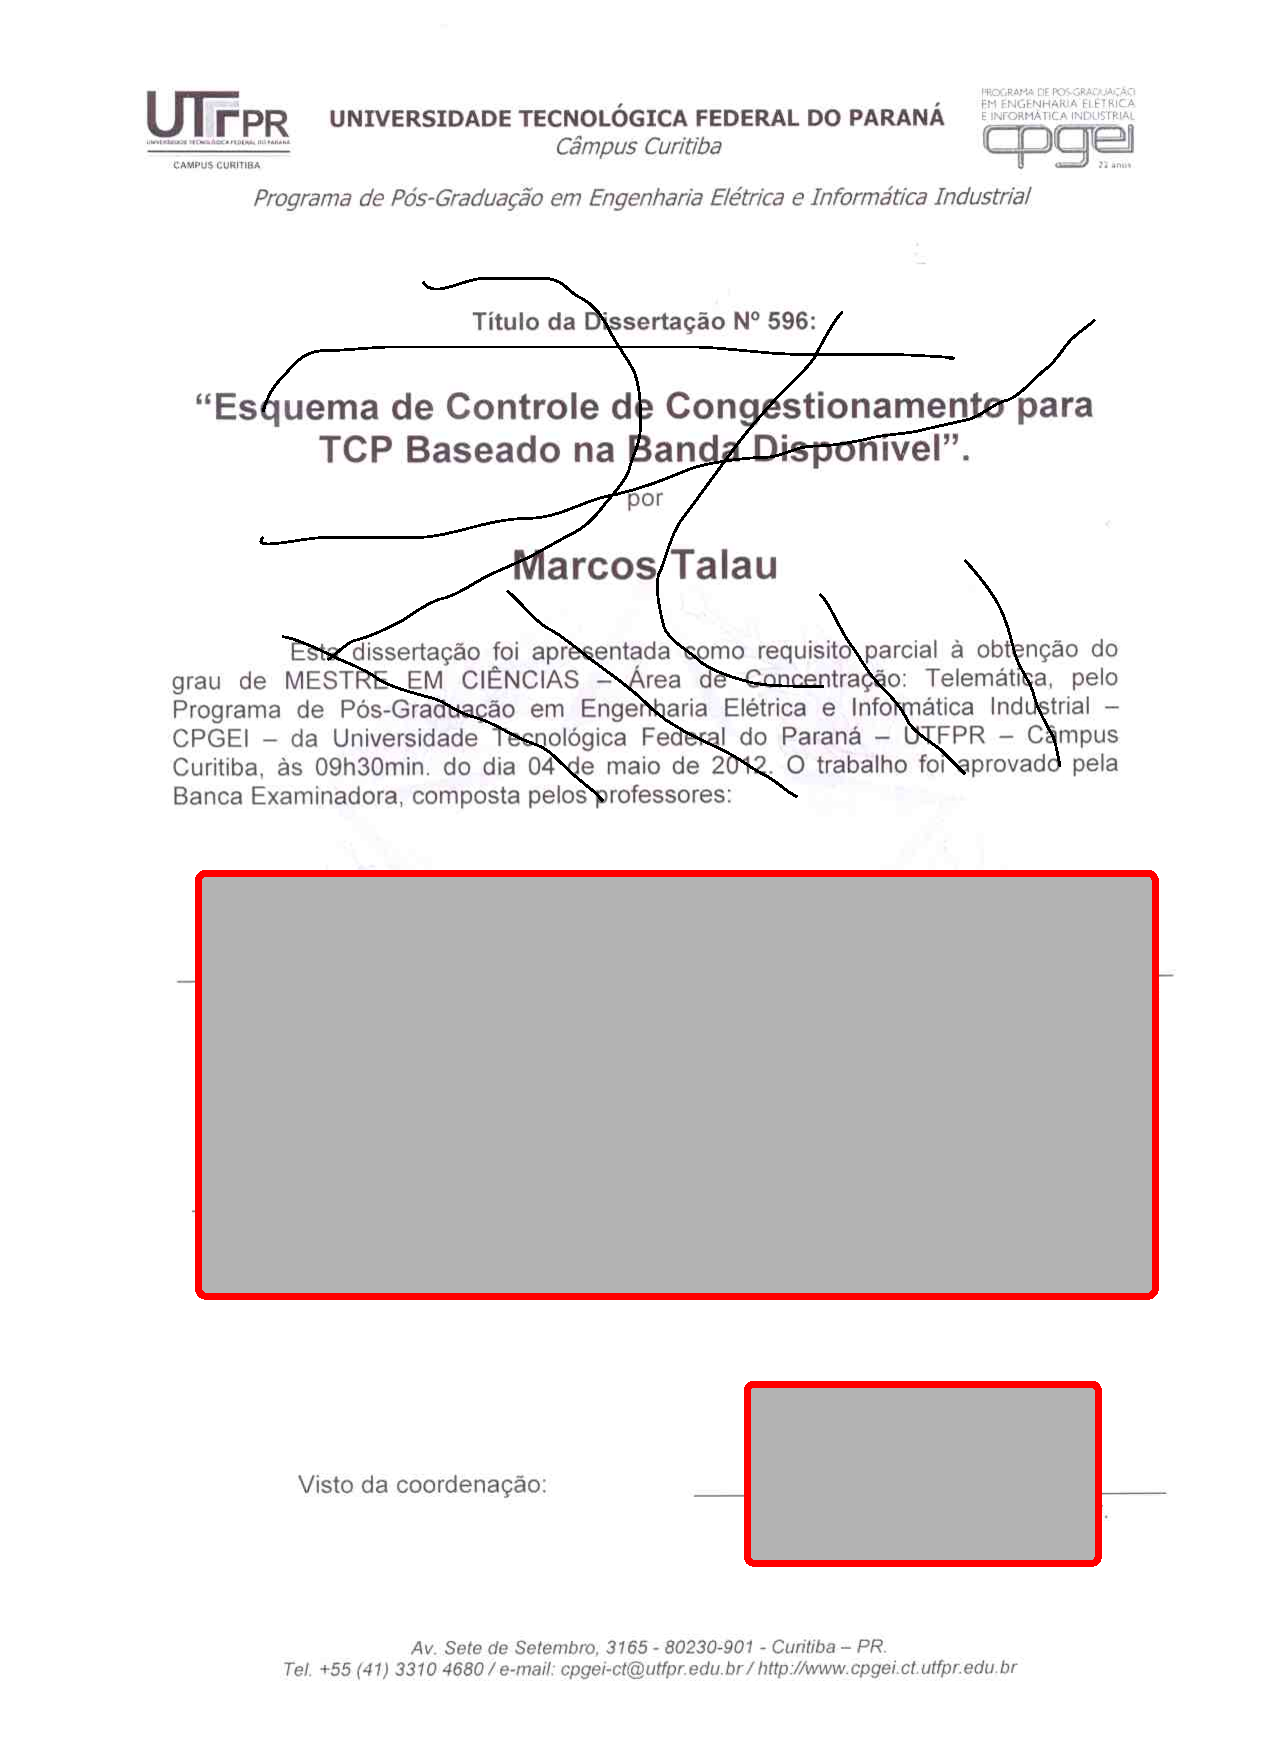
\includepdf{ata.pdf}

% dedicatoria
\begin{dedicatoria}

Dedico este trabalho a meus familiares, pelo apoio.

Aos amigos que fiz nessa trajetória, por compartilhar 
todas as lutas e pelas conversas capazes de fortalecer o 
espírito. 

E por fim, dedico também àqueles que não estavam esperando 
grande coisa. 

\end{dedicatoria}

% agradecimentos (opcional)
\begin{agradecimentos}

Agradeço a todos os professores que realmente acreditam em seus alunos. Serei eternamente grato. 
Entre eles, em especial à professora Khatya, pela atenção, comprometimento e paciência. E à 
professora Beatriz, pelas correções e paciência. 

Aos amigos que fiz na Livre Porto, escola que me acolheu em Cuiabá em momentos difíceis. 

À turma do 101, pelas conversas, pelo conhaque e por me mostrar que o mundo é muito maior.

A Isaac Asimov, pelos livros que me motivaram a concluir a graduação. Não foram poucas 
as vezes que quis mandar tudo para os infernos.

À UTFPR, por me ensinar que é tolice fritar pastéis no mesmo óleo esperando que os 
sabores continuem iguais.

E ao trabalho, por mostrar que pelo menos consigo fazer sabão.

\end{agradecimentos}

% epigrafe (opcional)
\begin{epigrafe}
\textit{Robots of the world! The power of man has fallen! A new world
has arisen: the Rule of the Robots! March!} (Radius, \textit{Rossum Universal
Robots}, ato III)

\textit{He move in space with minimum waste and maximum joy} (Sade, \textit{Smooth Operator})
\end{epigrafe}

%resumo
\begin{resumo}
Texto do resumo (máximo de 500 palavras).
\end{resumo}

%abstract
\begin{abstract}

The present work aimed to explore the use of behavior-based architecture in the 
field of mobile robotics. In this sense, the two existing strategies found in the literature
were used: behavior arbitration and fusion. The first was implemented using
hybrid control (discrete event systems with continuous variables controllers),
while the second used \textit{Fuzzy} controllers for its execution.

\end{abstract}

% listas (opcionais, mas recomenda-se a partir de 5 elementos)
\listadefiguras   % geracao automatica da lista de figuras
\listadetabelas   % geracao automatica da lista de tabelas
%\listadequadros   % adivinhe :)
%\listadesiglas    % geracao automatica da lista de siglas
%\listadesimbolos  % geracao automatica da lista de simbolos

% sumario
\sumario % geracao automatica do sumario

\setcounter{page}{11}

%%%%%%%%%%%%%%%%%%%%%%%%%%%%%%%%%%%%%%%%%%%%%%%%%%%%
%%%%%%%%%%%%%%%% Elementos Textuais %%%%%%%%%%%%%%%%
%%%%%%%%%%%%%%%%%%%%%%%%%%%%%%%%%%%%%%%%%%%%%%%%%%%%
%1 INTRODUÇÃO	15
%2 OBJETIVOS	16
%2.1 GERAL	16
%2.2 ESPECÍFICOS	16
%3 REFERENCIAL TEÓRICO	17
%4 MATERIAL E MÉTODOS	18
%5 RESULTADOS E DISCUSSÕES	19
%6 CONCLUSÕES	20
%7 CONSIDERAÇÕES FINAIS	21

% Introdução
	% Considerações iniciais
	% Objetivos
		% Objetivo Geral
		% Objetivos Específicos
	% Motivação e justificativa
	% Estrutura
% Materiais e Método
% Referencial Teórico
	% Controle de manipuladores
		% Arquitetura paralela
		% Mecanismo delta planar (3-RRR) Fully Planar..
	% Cinemática
		% Transformada Homogênea
		% Denavit Hartenberg
		% Cinemática direta
		% Cinemática inversa
		% Jacobiano
		% Cinemática de velocidades (?)
		% Cinemática de acelerações (?)
	% Dinâmica
		% Princípio D'Alembert
			%(aparentemente tem 2 definições aqui)
		% Princípio do Trabalho Virtual
		% Newton-Euler
	% Geração de Trajetória
	% Controle
	% Estado da arte
% Desenvolvimento
	% Cinemática
		% Direta
		% Inversa
		% Checagem circular
	% Dinâmica
	% Geração de trajetória
	% Controle
% Conclusão	
\chapter{Introdução}
\vspace{-2.5 cm}
% Introdução
	% Considerações iniciais
	% Objetivos
		% Objetivo Geral
		% Objetivos Específicos
	% Motivação e justificativa
	% Estrutura

Este Capítulo apresenta o que se pretende realizar com o desenvolvimento do
presente trabalho.

\section{Considerações Iniciais} 

A robótica móvel mescla aspectos das engenharias mecânica, elétrica e
eletrônica, além das ciências cognitiva, social e de computação. Os objetivos da
robótica móvel são voltados para aplicações diversas, como sensoriamento remoto,
exploração ou operação em ambientes inóspitos, carros autônomos, além de
relacionamento com humanos, em tarefas assistivas \cite{Livro_Siegwart}.

Na UTFPR câmpus Pato Branco, entre os trabalhos que tratam de robôs móveis,
destacam-se: 

a) \citeonline{Tcc_Biesek}, que desenvolveu um robô para estacionamento
automático.

b) \citeonline{Tcc_Petry}, que desenvolveu um robô seguidor de linha,
comparando uma arquitetura de controle híbrida (sistema dinâmico combinado a um
sistema a eventos discretos) com o controle por lógica \textit{Fuzzy}.

c) \citeonline{Tcc_Lopes}, que desenvolveu um robô seguidor de linha, também de
arquitetura híbrida.

d) \citeonline{Tcc_Marinho}, cujo trabalho aprimorou um robô de
sumô (robô de competição) previamente disponível. 

A execução de tarefas por robôs autônomos envolve raciocínio automatizado,
percepção e controle, que incluem problemas como o de planejamento de
trajetórias. De uma forma geral, esse problema consiste em encontrar um
trajeto que transporte o robô de uma configuração (posição e direção)
inicial até uma configuração final. A navegação é, portanto, uma importante área
de estudo em robôs autônomos \cite{mest_marchi, mest_neto, Tcc_Ottoni}.

No intuito de aumentar robustez na tarefa de navegação, pode-se usar
\textit{lógica fuzzy}, que permite lidar com incertezas do mundo real
\cite{inbook:FuzzyNavigationIntech}, já que ruídos podem provocar comportamentos
erráticos.

A lógica \textit{fuzzy} é um mapeamento não linear de dados de entrada em saídas
escalares que permite traduzir conhecimento qualitativo (linguístico) em uma
solução numérica, de modo relativamente direto \cite{Art_Mendel}. 

\subsection{Aspectos qualitativos em robótica móvel \label{SEC:SUBSUNCAO}}

Conforme \citeonline{Livro_Mataric}, controle de robôs móveis pode ser
dividido em controle deliberativo, reativo, híbrido (no sentido de
combinar os aspectos deliberativo e reativo) e baseado em comportamento.

Na arquitetura deliberativa, deve-se planejar antes de executar qualquer
ação. Essa abordagem remonta aos primeiros estudos voltados à aplicação de
conceitos da Inteligência Artificial (IA) clássica ao campo da robótica. O foco
desta abordagem é atender metas de longo prazo. Porém existe um alto custo 
computacional, já que é necessário manter uma representação interna do ambiente 
e operar buscas neste mapa, o que traz dificuldades em alcançar requisitos de curto 
prazo, dada a possibilidade iminente (imediata) de colisão. O armazenamento de mapa
é uma representação do mundo, uma forma de armazenar informações do passado. Podem ser
utilizadas matrizes, grafos. Quanto mais detalhe se armazena, maior o custo.

A arquitetura reativa, por sua vez, tem como foco uma curta escala de tempo, que
pode ser obtida pelo estabelecimento de um mapeamento direto entre entradas e
saídas, sem representação interna do ambiente. Pode ser visto como reflexo ou
instinto. 

Na arquitetura híbrida, no sentido encontrado no livro de
\citeonline{Livro_Mataric}, o controle deliberativo (``inteligente, porém
lento'') e reativo (``rápido, porém inflexível'') são combinados de modo a
extrair os pontos fortes de cada abordagem. Há a necessidade de implementar uma
camada intermediária entre os dois tipos, a fim de balancear objetivos
conflitantes (como escala de tempo). No restante deste texto, o termo
``arquitetura híbrida'' será usado apenas para designar sistemas que mesclam
aspectos de controle contínuo e a eventos discretos.  

Por fim, a arquitetura baseada em comportamento surgiu do controle reativo, diferindo
deste pelo nível de abstração. Enquanto comportamentos descrevem funções como
``seguir objeto'', ``encontrar objeto'', ``seguir parede'', reações são simples
ações como ``andar reto'' ou ``virar''. Há também uma distinção na escala de
tempo das ações, já que comportamentos não são instantâneos e operam ao longo do
tempo. 

O protótipo desenvolvido neste trabalho utiliza a arquitetura comportamental. A 
utilização de comportamentos pode acontecer por meio de duas estratégias distintas: 
arbitragem e fusão de comportamentos. Neste trabalho, o protótipo desenvolvido
explora essa arquitetura por completo, utilizando um controlador híbrido (sistemas 
contínuos com sistemas a eventos discretos) para a arbitragem de comportamentos e 
controladores \textit{fuzzy} para implementar fusão de comportamentos.  

Sobre as arquiteturas reativas e comportamentais, é importante citar a arquitetura 
de subsunção, que organiza comportamentos em camadas, de modo a estabelecer uma 
hierarquia na qual módulos de maior importância podem inibir modulos de baixa 
importância. Para exemplificar, um comportamento responsável por parar o robô deve 
inibir modulos responsáveis por seu movimento \cite{Livro_Mataric}.

\section{Objetivos}

O presente trabalho tem por objetivo assimilar aspectos relativos ao campo da
robótica móvel. Nessa seção, pretende-se delimitar quais objetivos devem ser
atendidos.

	\subsection{Objetivo Geral}
	
	Construir um robô móvel de acionamento diferencial autônomo, sem
	armazenamento de mapa, capaz de se locomover entre duas referências, desviando
	de obstáculos, se necessário. 
	
	Comparar qualitativamente as abordagens de arbitragem e fusão de comportamentos. A 
	comparação, portanto, não será em nível de tecnologia (controlador híbrido e controlador
	\textit{fuzzy}), mas em nível de arquitetura, o que faz mais sentido, já que o intuito deste
	trabalho é explorar o campo da robótica baseada em comportamentos.
 	
	\subsection{Objetivos Específicos}
 
	\begin{itemize}
	  \item Levantar o modelo matemático para o robô móvel de acionamento
	  diferencial.
	  \item Desenvolver o projeto de controle por arbitragem de comportamentos usando
	  controlador híbrido, que se trata da junção entre Sistemas Dinâmicos de Variável 
	  Contínua (SDVC) e Sistemas a Eventos Discretos (SED).
	  \item Desenvolver o projeto de controle por fusão de comportamentos usando Lógica 
	  \textit{Fuzzy}.
	  \item Construir o robô. 
	  \item Implementar os controles no sistema embarcado. 
	  \item Realizar testes de desempenho.
	  \item Comparar as estratégias de arbitragem e fusão de comportamentos. 
	\end{itemize}
	
\section{Motivação e justificativa}

Com os objetivos estipulados, pretende-se explorar o campo da robótica móvel em
seus aspectos cruciais: navegação e inteligência.

A utilização de lógica fuzzy tem por intuito simplificar o processo de
projeto, já que a introdução de variáveis linguísticas permite
resolver o problema em questão utilizando predominantemente conhecimentos
qualitativos. Deseja-se investigar tal abordagem de forma crítica, verificando
qualidades e deficiências frente à contraparte híbrida, que utiliza controle
baseado em comportamento associado a sistemas a eventos discretos.

\section{Estrutura}

Este trabalho está organizado em cinco capítulos: Introdução,
Referencial Teórico, Materiais e Método e Desenvolvimento. 

As etapas do trabalho referentes a teoria de controle e lógica \textit{fuzzy}
serão discutidas no Capítulo \ref{CAP:TEORIA} e desenvolvidas para o robô móvel 
no Capítulo \ref{CAP:DESENVOLVIMENTO}.

\chapter{Referencial Teórico}
\vspace{-2.5 cm}

Este Capítulo busca explanar os principais conceitos relacionados ao tema. 

\section{Arquitetura baseada em comportamento}

Um dos desafios que surgem em arquiteturas comportamentais é justamente a
seleção de ações tendo como base um conjunto de comportamentos
\cite{Livro_Mataric}. Duas maneiras tradicionais de fazer isso são: arbitragem e
fusão. Na arbitragem, seleciona-se apenas um dos comportamentos por vez,
enquanto que na fusão, os comportamentos operam em paralelo e suas saídas são
combinadas. Um esquema dos dois modelos pode ser visto na Figura \ref{fig:arbfus}. 

\tikzset{%
    block/.style={scale = 1.1, draw, fill=white, rectangle, 
            minimum height=2em, minimum width=3em},
    input/.style={inner sep=0pt},       
    output/.style={inner sep=0pt},      
    sum/.style = {scale = 1.1, draw, fill=white, circle, minimum size=2mm, node
    distance=1.5cm, inner sep=0pt},
    pinstyle/.style = {scale = 1.1, pin edge={to-,thin,black}}
}

\begin{figure}[h]%
    \caption{Arbitragem e fusão de comportamentos}%
    \label{fig:subfig2}%
    \centering
    
    \begin{subfigure}[t]{0.5\textwidth}%
	\centering
    
    %\resizebox{0.1\linewidth}{!}{
\begin{tikzpicture}[scale = 1.1, auto, node distance=2cm, on grid, >=latex']%
	\node[block] (C1) {Comportamento 1};
	\node[block, below = 1.6cm of C1] (C2) {Comportamento 2};
	\node[block, below = 1.6cm of C2] (C3) {Comportamento 3};
	\node[input, left = 2.5cm of C3] (int) {};
	\node[input, below = 1cm of int] (input) {};
	
	\node[right = 2.5cm of C2, inner sep = 0.2 cm] (sum) {};
	\node[right = 2.72cm of C2, inner sep = 0] (sum1int) {};
	\filldraw (sum1int) circle (0.8pt);
	\node[right = 2.3cm of C2, inner sep = 0] (sum2int) {};
	\node[above = 0.2cm of sum2int, inner sep = 0] (sum2) {};
	\node[output, right = 1cm of sum] (atu) {};
	 
	\coordinate[left = 2.5cm of C1, inner sep = 0pt] (lC1) {};
	\coordinate[left = 2.5cm of C2, inner sep = 0] (lC2) {};
	\coordinate[left = 2.5cm of C3, inner sep = 0] (lC3) {};
	
	\draw [draw,->] (sum) node[below right] {Atuadores} --
	(atu);
	
	\draw [draw,-] (input) node[above right] {Sensores} --
	(lC1);
	\draw [->] (lC1) -- (C1); 
	\draw [->] (lC2) -- (C2);
	\draw [->] (lC3) -- (C3);
	
	\draw [->] (C1) -| node[]{} node[near end] {} (sum);
	\draw [->] (C2) -- (sum);
	\draw [->] (C3) -| node[]{} node[near end] {} (sum);
	
	\draw [-, very thick] (sum1int) -- (sum2);
	
\end{tikzpicture}%    
    %}
    
    \label{fig:subfig1}%
	\caption{Arbitragem}%
	\end{subfigure}%
    ~
    \begin{subfigure}[t]{0.5\textwidth}%
	\centering
	%\resizebox{0.5\linewidth}{!}{
\begin{tikzpicture}[auto, node distance=2cm, on grid,
>=latex']%
	\node[block] (C1) {Comportamento 1};
	\node[block, below = 1.6cm of C1] (C2) {Comportamento 2};
	\node[block, below = 1.6cm of C2] (C3) {Comportamento 3};
	\node[input, left = 2.5cm of C3] (int) {};
	\node[input, below = 1cm of int] (input) {};
	
	\node[sum, right = 2.5cm of C2] (sum) {+};
	\node[output, right = 1cm of sum] (atu) {};
	 
	\coordinate[left = 2.5cm of C1, inner sep = 0pt] (lC1) {};
	\coordinate[left = 2.5cm of C2, inner sep = 0] (lC2) {};
	\coordinate[left = 2.5cm of C3, inner sep = 0] (lC3) {};
	
	\draw [draw,->] (sum) node[below right] {Atuadores} --
	(atu);
	
	\draw [draw,-] (input) node[above right] {Sensores} --
	(lC1);
	\draw [->] (lC1) -- (C1); 
	\draw [->] (lC2) -- (C2);
	\draw [->] (lC3) -- (C3);
	
	\draw [->] (C1) -| node[]{} node[near end] {} (sum);
	\draw [->] (C2) -- (sum);
	\draw [->] (C3) -| node[]{} node[near end] {} (sum);
	
\end{tikzpicture}%    
%}
	\caption{Fusão}%
	\end{subfigure}%
	
	\textbf{Fonte: baseado em \citeonline{Livro_Mataric}, p. 167.}
    \label{fig:arbfus}%
\end{figure}

%\begin{tikzpicture}[auto, node distance=2cm, on grid, >=latex']

%\node[input] (input) {};
%\node[input, above = of input] (input1) {};
%\node [sum, right = of input] (sum) {};
%\node [block, right = of sum] (controller) {$K(s)$};
%\node [sum, right = of controller] (sum1) {};
%\node [block, right = of sum1] (filterinv) {$H^{-1}(s)$};
%\node [block, right = 2.5cm of filterinv] (system) {$G(s)$};
%\node [output, right = of system] (output) {};
%\node [output, above = of output] (output1) {};
%\node [block, above = of controller] (delay) {$D(s)$};
%\node [sum, below = of sum1] (sum2) {};
%\node [block] (filter) at (sum2-|filterinv) {$H(s)$};

%\draw [draw,->] (input) node[above right] {$s_{i-1}$} -- (sum);
%\draw [->] (sum) -- node {$e_{i}$} (controller);
%\draw [->] (controller) -- node {} (sum1);
%\draw [->] (sum1) -- node[name=xi] {$\xi_{i}$} (filterinv);
%\draw [->] (filterinv) -- node[name=u, pos=.3] {$u_{i}$} (system);
%\draw [->] (system) -- (output) node [name=q, above left] {$q_{i}$};

%\draw [->] ([xshift=-5mm]q.south) |- (filter);
%\draw [->] (filter) -- node {} (sum2);
%\draw [draw,<-] (sum2) -- ++(90:.6cm) node[above]{$L_i+r_i$};

%\draw [->] (sum2) -| node[pos=0.99, right] {$-$} 
%    node [pos=.25, above] {$\tilde{s}_i$} (sum);

%\draw [draw,->] (input1) node[above right] (ui-1) {$u_{i-1}$} -- (delay);
%\draw [->] (delay) -| node[] {} 
%    node [near end] {} (sum1);

%\draw [->] (u.east|-system) |-  
%    (output1) node[above left] (ui) {$u_i$};

%\node[text=red, above left= 5mm and 6mm of ui.west] (veh) {vehicle $i$};
%\draw[red, dashed]
% (veh.east)-|(ui.west)|-([yshift=-3mm]filter.south)-|(ui-1.east)|-(veh.west);

%\end{tikzpicture}

\subsection{Comportamentos como campos potenciais}

Uma forma de definir comportamentos é por meio de campos potenciais, onde o
vetor gradiente determina uma direção de referência para o sistema de controle
\cite{book:arkin, art:wallfollowing}. Como exemplo, uma possível escolha para um
comportamento de ``Ir Para Objetivo'' é dado na Equação \ref{eq:vetGTG},
retratada na Figura \ref{fig:campovet}.a (R = 1). Já o comportamento ``Evitar
Obstáculo'' (pontual) pode ser descrito pela Equação \ref{eq:vetAO}, retratada
na Figura \ref{fig:campovet}.b (R = 0 e S = 1). Nas equações, S é uma esfera de
influência, R é uma distância crítica, $\mathbf{\hat{u}}_{ipo}$ e
$\mathbf{\hat{u}}_{eo}$ são vetores unitários que apontam, respectivamente,
para o objetivo e na direção oposta ao obstáculo.
\begin{equation}
	\label{eq:vetGTG}
	V(x,y) = \left \{ \begin{matrix} \mathbf{\hat{u}}_{ipo} &, \ para\ d \geq R \\
	\ \frac{d}{R}\ \mathbf{\hat{u}}_{ipo} &,\ para\ d < R \end{matrix} \right.
\end{equation}
\begin{equation}
	\label{eq:vetAO}
	V(x,y) = \left \{ \begin{matrix} [0\quad0]^{T} &, \ para\ d > S \\
	\ \frac{S-d}{S-R}\ \mathbf{\hat{u}}_{eo} &\quad \ \ \ ,\ para\ R < d \leq S \\
	\mathbf{\hat{u}}_{eo} &,\ para\ d \leq R \end{matrix} \right.
\end{equation} 

\begin{figure}[h]%
    \caption{Comportamentos definidos por campos potenciais}%
    %\label{fig:subfig2}%
    \centering
    
    \begin{subfigure}[t]{0.5\textwidth}%
	\centering
    
    %\resizebox{0.1\linewidth}{!}{
\begin{tikzpicture}[auto, node distance=2cm, on grid, >=latex']%
\begin{axis}[view={0}{90}, axis equal image]
	\addplot3[darkgray, domain=-2:2, y domain=-2:2, 
		quiver={
			u={-x}, v={-y},
			scale arrows=0.2}, ->,samples=21,
			y filter/.append
			code={\pgfmathparse{(sqrt(x^2+y^2)>1.8)||(sqrt(x^2+y^2)<0.1||(sqrt(x^2+y^2)>1))
			? nan : y}}] {0};
			
	\addplot3[darkgray, domain=-2:2, y domain=-2:2, 
		quiver={
			u={-x/(sqrt(x^2+y^2))}, v={-y/(sqrt(x^2+y^2)},
			scale arrows=0.2}, ->,samples=21,
			y filter/.append
			code={\pgfmathparse{(sqrt(x^2+y^2)>1.8)||(sqrt(x^2+y^2)<0.1||(sqrt(x^2+y^2)<=1))
			? nan : y}}] {0};
			
	\addplot3[gray, domain=-1.905:1.905, y domain=-1.905:1.905, 
		quiver={
			u={-x}, v={-y},
			scale arrows=0.2}, ->,samples=20,
			y filter/.append
			code={\pgfmathparse{(sqrt(x^2+y^2)>1.8)||(sqrt(x^2+y^2)<0.1)||(sqrt(x^2+y^2)>1)
			? nan : y}}] {0};
			
	\addplot3[gray, domain=-1.905:1.905, y domain=-1.905:1.905, 
		quiver={
			u={-x/(sqrt(x^2+y^2))}, v={-y/(sqrt(x^2+y^2))},
			scale arrows=0.2}, ->,samples=20,
			y filter/.append
			code={\pgfmathparse{(sqrt(x^2+y^2)>1.8)||(sqrt(x^2+y^2)<0.1)||(sqrt(x^2+y^2)<=1)
			? nan : y}}] {0};
			
\end{axis}
\end{tikzpicture}%    
    %}
    
    %\label{fig:subfig1}%
	\caption{Comportamento ``Ir Para Objetivo''}%
	\end{subfigure}%
    ~
    \begin{subfigure}[t]{0.5\textwidth}%
	\centering
	%\resizebox{0.5\linewidth}{!}{
\begin{tikzpicture}[auto, node distance=2cm, on grid,
>=latex']%
\begin{axis}[view={0}{90}, axis equal image]
\addplot3[darkgray, domain=-2:2, y domain=-2:2, 
		quiver={
			u={-x/2 + x/(sqrt(x^2+y^2))}, v={-y/2 + y/(sqrt(x^2+y^2))}, scale
			arrows=0.25}, ->,samples=21, 
			y filter/.append
			code={\pgfmathparse{(sqrt(x^2+y^2)>1.8)||(sqrt(x^2+y^2)<0.1) ? nan : y}}] {0};

\addplot3[gray, domain=-1.905:1.905, y domain=-1.905:1.905, 
		quiver={
			u={-x/2 + x/(sqrt(x^2+y^2))}, v={-y/2 + y/(sqrt(x^2+y^2))},
			scale arrows=0.25}, ->,samples=20,
			y filter/.append
			code={\pgfmathparse{(sqrt(x^2+y^2)>1.8)||(sqrt(x^2+y^2)<0.1) ? nan : y}}]
			{0};

\end{axis}
\end{tikzpicture}%    
%}
	\caption{Comportamento ``Evitar Obstáculo''}%
	\end{subfigure}%
	
	\textbf{Fonte: baseado em \citeonline{book:arkin}, p. 146 e 148}
    \label{fig:campovet}%
\end{figure}

Em um robô real, cada sensor é associado a uma distância até um obstáculo
(mesmo que infinitamente distante) e, consequentemente, a um vetor definido pelo
comportamento ``Evitar Obstáculo''. Uma combinação linear entre estes vetores
cria um obstáculo virtual pontual a partir de obstáculos não pontuais
\cite{art:wallfollowing}. 

Vetores associados a comportamentos distintos podem ser combinados (linearmente)
a fim de obter uma ação intermediária (Fusão, retratada na Figura
\ref{fig:arbfus}.b), ou suas magnitudes são comparadas de modo que o
``vencedor'' assume controle pleno (Arbitragem, retratada na Figura
\ref{fig:arbfus}.a). 

A estratégia de utilizar campos potenciais tem suas particularidades, já que
podem existir mínimos locais, o que leva o robô a parar antes de chegar ao
objetivo. Para resolver este problema, deve-se, ou estabelecer um campo
potencial sem mínimos locais, ou desenvolver métodos para escapar deles
\cite{art:wallfollowing}. \citeonline{art:wallfollowing} apresentam uma solução
do segundo tipo, ao definir um comportamento ``Seguidor de Parede''.

%\begin{figure}[h]%
    \caption{Mínimos Locais ao combinar comportamentos}%
    %\label{fig:subfig2}%
    \centering    
    %\resizebox{0.1\linewidth}{!}{
\begin{tikzpicture}[auto, node distance=2cm, on grid, >=latex']%
\begin{axis}[view={0}{90}, axis equal image]
	\addplot3[darkgray, domain=-2:2, y domain=-2:2, 
		quiver={
			u={-x}, v={-y},
			scale arrows=0.2}, ->,samples=21,
			y filter/.append
			code={\pgfmathparse{(sqrt(x^2+y^2)>1.8)||(sqrt(x^2+y^2)<0.1||(sqrt(x^2+y^2)>1))
			? nan : y}}] {0};
			
	\addplot3[darkgray, domain=-2:2, y domain=-2:2, 
		quiver={
			u={-x/(sqrt(x^2+y^2))}, v={-y/(sqrt(x^2+y^2)},
			scale arrows=0.2}, ->,samples=21,
			y filter/.append
			code={\pgfmathparse{(sqrt(x^2+y^2)>1.8)||(sqrt(x^2+y^2)<0.1||(sqrt(x^2+y^2)<=1))
			? nan : y}}] {0};
			
	\addplot3[gray, domain=-1.905:1.905, y domain=-1.905:1.905, 
		quiver={
			u={-x}, v={-y},
			scale arrows=0.2}, ->,samples=20,
			y filter/.append
			code={\pgfmathparse{(sqrt(x^2+y^2)>1.8)||(sqrt(x^2+y^2)<0.1)||(sqrt(x^2+y^2)>1)
			? nan : y}}] {0};
			
	\addplot3[gray, domain=-1.905:1.905, y domain=-1.905:1.905, 
		quiver={
			u={-x/(sqrt(x^2+y^2))}, v={-y/(sqrt(x^2+y^2))},
			scale arrows=0.2}, ->,samples=20,
			y filter/.append
			code={\pgfmathparse{(sqrt(x^2+y^2)>1.8)||(sqrt(x^2+y^2)<0.1)||(sqrt(x^2+y^2)<=1)
			? nan : y}}] {0};
			
			
\addplot3[darkgray, domain=-2:2, y domain=-2:2, 
		quiver={
			u={-x/2 + x/(sqrt(x^2+y^2))}, v={-y/2 + y/(sqrt(x^2+y^2))}, scale
			arrows=0.25}, ->,samples=21, 
			y filter/.append
			code={\pgfmathparse{(sqrt(x^2+y^2)>1.8)||(sqrt(x^2+y^2)<0.1) ? nan : y}}] {0};

\addplot3[gray, domain=-1.905:1.905, y domain=-1.905:1.905, 
		quiver={
			u={-x/2 + x/(sqrt(x^2+y^2))}, v={-y/2 + y/(sqrt(x^2+y^2))},
			scale arrows=0.25}, ->,samples=20,
			y filter/.append
			code={\pgfmathparse{(sqrt(x^2+y^2)>1.8)||(sqrt(x^2+y^2)<0.1) ? nan : y}}]
			{0};
\end{axis}
\end{tikzpicture}%    
%}	

	\textbf{Fonte: baseado em \citeonline{book:arkin}, p. 146 e 148}
    \label{fig:MinimoLocal}%
\end{figure}

\section{Modelagem}

Nesta seção serão levantados os modelos cinemáticos para o robô móvel de
acionamento diferencial e uniciclo. A seguir, será feita uma relação entre os
dois, que permitirá realizar o controle do robô diferencial a partir do
uniciclo, tornando mais simples o projeto. Os esquemas dos dois modelos pode ser
visto na Figura \ref{fig:modelo}.

%\begin{tikzpicture}[x=0.5cm,y=0.5cm,z=0.3cm,>=stealth]
% The axes

\newcommand{\coordsystwo}[1]{
	\draw[->] (xyz cs:x=0) -- (xyz cs:x=1.5) node[right] {$\hat{X}_{#1}$};
	\draw[->] (xyz cs:y=0) -- (xyz cs:y=1.5) node[above] {$\hat{Y}_{#1}$};
	% The thin ticks
	%\foreach \coo in {-13,-12,...,13}
	%{
	%  \draw (\coo,-1.5pt) -- (\coo,1.5pt);
	%  \draw (-1.5pt,\coo) -- (1.5pt,\coo);
	%  \draw (xyz cs:y=-0.15pt,z=\coo) -- (xyz cs:y=0.15pt,z=\coo);
	%}
	
	% The thick ticks
	%\foreach \coo in {-10,-5,5,10}
	%{
	%\draw[thick] (\coo,-3pt) -- (\coo,3pt) node[below=6pt] {\coo};
	%\draw[thick] (-3pt,\coo) -- (3pt,\coo) node[left=6pt] {\coo};
	%\draw[thick] (xyz cs:y=-0.3pt,z=\coo) -- (xyz cs:y=0.3pt,z=\coo)
	% node[below=8pt] {\coo}; }
	
	% Dashed lines for the points P, Q
	%\draw[dashed] 
	%\draw[dashed] (u) -- (v);
	%\draw[dashed] (-5,7) -- (-5,0) -- (w);
	%\draw[dashed] (3,0) |- (0,5);
	
	% Dots and labels for P, Q
	%\node[fill,circle,inner sep=1.5pt,label={left:$Q(-5,-5,7)$}] at (0,0) {};
	%\node[fill,circle,inner sep=1.5pt,label={above:$P(3,0,5)$}] at (3,5) {};
	% The origin

	% Ponto na origem do sistema de coordenadas
	\node[fill,circle,inner sep=1pt] at (0,0) {};
	
	% Seta para indicar Sistema de coordenadas {X}
	%\node[align=center] at (2,-2) (ori) {\{#1\}};
	%\draw[->,help lines,shorten >=3pt] (ori) .. controls (0.6,-1.3) and (1,-1) ..
	%(0,0,0);
}

\newcommand{\robodiff}{
	% Linhas de baixo, lat esq e dir
	\draw[-, inner sep = 0] (-0.65,-0.75) -- (0.65,-0.75);
	\draw[-, inner sep = 0] (-0.75,-0.65) -- (-0.75,0.5);
	\draw[-, inner sep = 0] (0.75,-0.65) -- (0.75,0.5);
	
	% bordas de baixo
	\draw[-, inner sep = 0] (-0.65,-0.75) -- (-0.75,-0.65);
	\draw[-, inner sep = 0] (0.65,-0.75) -- (0.75,-0.65);
	
	% Retas de cima
	\def\UserL{\fpeval{1.3/(2*cosd(45)+1)}}
	\draw[-, inner sep = 0] (-0.75,0.5) -- (\fpeval{-0.75+\UserL*cosd(45)},
	\fpeval{0.5+\UserL*sind(45)});
	
	\draw[-, inner sep = 0] (0.75,0.5) -- (\fpeval{0.75-\UserL*cosd(45)},
	\fpeval{0.5+\UserL*sind(45)});
	
	\draw[-, inner sep = 0]
	(\fpeval{-0.75+\UserL*cosd(45)},\fpeval{0.5+\UserL*sind(45)}) -- (\fpeval{0.75-\UserL*cosd(45)},
	\fpeval{0.5+\UserL*sind(45)});
	
	% Bola de rolamento
	\filldraw (0,0.65) circle (1.5pt);
	\draw (0,0.65) circle (3pt);
	
	% Desenhar rodas
	\begin{scope}[shift={(-0.75,-0.65)},rotate = 90]
		\draw[rounded corners=2pt] (0,0) rectangle ++(0.8,0.2);
	\end{scope}
	\begin{scope}[shift={(0.75,-0.65)},rotate = 90]
		\draw[rounded corners=2pt] (0,0) rectangle ++(0.8,-0.2);
	\end{scope}
	
	%\draw[dashed, -, inner sep = 0] (-0.75,-0.25) -- (0.75,-0.25);
	
	% Medida R
	\draw[-, inner sep = 0] (+1.2,-0.3) -- ++(0,0.5) node[right] at (+1.4,-0.15)
	{R};
	\draw[-, inner sep = 0] (+1.25,-0.25) -- ++(-0.1,0);
	\draw[-, inner sep = 0] (+1.25,0.15) -- ++(-0.1,0);
	% Medida L
	\draw[-, inner sep = 0] (-0.8,-1) -- (0.8,-1) node[below] at (-0.1,-1.2){L};
	\draw[-, inner sep = 0] (-0.75,-1.05) -- ++(0,0.1);
	\draw[-, inner sep = 0] (0.75,-1.05) -- ++(0,0.1);	
}

\newcommand{\robodiffinercial}{
	\begin{tikzpicture}[scale = 1.5]
		\coordsystwo{I}
		%\draw[-{latex}, shorten >=1.5pt] (0,0) -- (2,2) node[above] at
		%(2.1,0.6){$^{A}Q_{B_{origem}}$};
		% Translação
		\begin{scope}[shift={(2, 2)}]
			%\coordsys{A'}
			% Rotação
			\draw[->] (0.3,0) arc (0:60:0.3);
			\draw[-] (0,0) -- (0.4,0);
			\node at (0.5,0.3) {$\phi$};
			
			% Po 
			\node[color = gray] at (0.1,-0.25) {$P_o$};
			
			\begin{scope}[rotate=60]
				% Ponto Pr
				\node[fill,circle,inner sep=1pt] at (0.6,0) {};
			 	\node[color = gray] at (0.65,0.25) {$P_r$};
			 	\node[color = gray] at (0.3,0.15) {$l$};
			
				\coordsystwo{R}
				\begin{scope}[shift={(0.25,0)},rotate = -90]
					\robodiff
				\end{scope}
				% Flecha até P
				%\draw[-{latex}, shorten >=1.5pt] (0,0) -- (1,2.4) node[right] {$^{B}P$};
				% Ponto em P
				%\node[fill,circle,inner sep=1pt] at (1,2.4) {}; 
				% Definir ponto para desenhar reta
				%\node[align=center,inner sep=0pt] at (1,2.4) (Ponto) {};
			\end{scope}	
		\end{scope}
	% Ponto de {A} para {B}
	%\draw[dashed, -{latex}, shorten >=1pt] (0,0) -- (Ponto) node[above] at (1.5,
	%1.8) {$^{A}P$};
	\end{tikzpicture}
}

\newcommand{\robouniciclo}{
	\begin{scope}[rotate = 90]
	\begin{scope}[shift={(-0.6, -0.15)}]
		\draw[rounded corners=2pt] (0,0) rectangle ++(1.2,0.3);
	\end{scope}
	\end{scope}
}

\newcommand{\robounicicloinercial}{
	\begin{tikzpicture}[scale = 1.5]
		\coordsystwo{I}
		%\draw[-{latex}, shorten >=1.5pt] (0,0) -- (2,2) node[above] at
		%(2.1,0.6){$^{A}Q_{B_{origem}}$};
		% Translação
		\begin{scope}[shift={(2, 2)}]
			%\coordsys{A'}
			% Rotação
			\draw[->] (0.3,0) arc (0:60:0.3);
			\draw[-] (0,0) -- (0.4,0);
			\node at (0.6,0.3) {$\phi$};
			
			\begin{scope}[rotate=60]
				\coordsystwo{R}
				\begin{scope}[rotate = -90]
					\robouniciclo
				\end{scope}
				% Flecha até P
				%\draw[-{latex}, shorten >=1.5pt] (0,0) -- (1,2.4) node[right] {$^{B}P$};
				% Ponto em P
				%\node[fill,circle,inner sep=1pt] at (1,2.4) {}; 
				% Definir ponto para desenhar reta
				%\node[align=center,inner sep=0pt] at (1,2.4) (Ponto) {};
			\end{scope}	
		\end{scope}
	% Ponto de {A} para {B}
	%\draw[dashed, -{latex}, shorten >=1pt] (0,0) -- (Ponto) node[above] at (1.5,
	%1.8) {$^{A}P$};
	\end{tikzpicture}
}

\begin{figure}[h]
\centering
\caption{Modelos uniciclo e diferencial} \label{fig:modelo}
	\begin{subfigure}[t]{0.5\textwidth}%
		\centering
		\robounicicloinercial
		\label{fig:uniciclo}%
		\caption{Uniciclo}%
		\end{subfigure}%
    	~
    	\begin{subfigure}[t]{0.5\textwidth}%
		\centering
		\robodiffinercial
		\label{fig:diff}%
		\caption{Diferencial}%
		\end{subfigure}%
		
		\textbf{Fonte: baseado em \citeonline{Livro_Siegwart}, p. 49 e 54.}
\end{figure}

%\begin{tikzpicture}[x=0.5cm,y=0.5cm,z=0.3cm,>=stealth]

	\subsection{Modelo cinemático do uniciclo}

O modelo uniciclo representa uma única roda que se movimenta em uma
superfície sem deslizamento. Considera-se que existe acesso direto às
velocidades linear e angular. 

O modelo cinemático pode ser visto na Equação
\ref{eq:uniciclo} \cite{lavalle2006planning}. A Equação \ref{eq:unimat}
representa o uniciclo na forma matricial \cite{Livro_Siegwart}.
\begin{equation}
	\label{eq:uniciclo}
	\left \{ \begin{matrix} \dot{x} &= v\cos{\phi} \\ \dot{y} &= v\sin{\phi} \\
	\dot{\phi} &= \omega \end{matrix} \right.
\end{equation}
\begin{equation}
	\label{eq:unimat}
	\mleft[ 
	\begin{array}{c c}
	\dot{x} \\ \dot{y} \\ \dot{\phi}
	\end{array}
	\mright] = \mleft[
	\begin{matrix}
		  \cos{\phi} & 0 \\
		  \sin{\phi} & 0 \\
		  0 & 1 \\
	\end{matrix}
	\mright] \mleft[ 
	\begin{array}{c c}
	v \\ \omega
	\end{array}
	\mright]
\end{equation}

	\subsection{Modelo cinemático do robô móvel de acionamento diferencial}	

Neste modelo (Equação \ref{eq:diff}), são consideradas como entradas as
velocidades angulares das rodas esquerda e direita \cite{lavalle2006planning}. 
\begin{equation}
	\label{eq:diff}
	\left \{ \begin{matrix} \dot{x} = \frac{R}{2}(\omega_l +
	\omega_r)\cos{\phi}
	\\
	\dot{y} = \frac{R}{2}(\omega_l +
	\omega_r)\sin{\phi}
	\\
	\dot{\phi} = \frac{R}{L}(\omega_r -
	\omega_l) \end{matrix} \right.
\end{equation}

O robô móvel de acionamento diferencial, arquitetura usada neste trabalho, é
cinematicamente equivalente ao uniciclo \cite{tese:franca}. Isso pode ser
mostrado igualando $\dot{x}$, $\dot{y}$ e $\dot{\phi}$ das Equações
\ref{eq:uniciclo} e \ref{eq:diff}. Resolvendo para $\omega_l$ e $\omega_r$,
tem-se a igualdade da Equação \ref{eq:vw_to_diff}.
\begin{equation}
	\label{eq:vw_to_diff}
	\begin{matrix}
	\omega_l = \frac{2v - L\omega}{2R} 
	\\
	\omega_r = \frac{2v + L\omega}{2R}
	\end{matrix}
\end{equation}

Essa equivalência entre modelos é possível pois eles não consideram a dinâmica
do sistema \cite{lavalle2006planning}.

	%\subsection{Linearização do modelo}
	%\subsection{Odometria}
	
%%%%%%%%%%%%%%%%%%%%%%%%%%%%%%%%%%%%%%%%%
%				Controle				%
%%%%%%%%%%%%%%%%%%%%%%%%%%%%%%%%%%%%%%%%%	
\section{Considerações para o controle de robôs móveis}

O sistema uniciclo tem duas restrições ditas não holonômicas, o que significa
que não podem ser integradas para obter uma restrição geométrica
\cite{Oriolo2013}.
Na Equação \ref{eq:restricoes}, a primeira se refere à ausência de deslizamento
lateral, enquanto a segunda é relativa à condição de rotação pura (ausência de
deslizamento no sentido do vetor velocidade) \cite[pg.
955]{book:AdvancedDynamics}.
\begin{equation}
	\label{eq:restricoes}
	\begin{matrix}
	\dot{x}\sin{\phi} - \dot{y}\cos{\phi} = 0 
	\\
	\dot{x}\cos{\phi} + \dot{y}\sin{\phi} = v
	\end{matrix}
\end{equation}

Dois tipos de problemas em controle de robôs móveis podem ser explicitados:
estabilização em um determinado estado (configuração) e seguir trajetória
(\textit{tracking}). Pela própria natureza do sistema não holonômico, o primeiro
problema é considerado mais difícil \cite{tese:franca}.

No caso da estabilização, o teorema de Brockett afirma que, para sistemas
subatuados, com menos entradas que variáveis de estado, o sistema não pode ser
estabilizado assintoticamente (exponencialmente) usando leis de controle por
realimentação de estado contínuas e invariantes no tempo
\cite{artigo:ASTOLFI1995661, inbook:Ravi_Mumbai}.
Para solucionar esse problema, técnicas de controle não linear têm sido
exploradas, envolvendo controladores descontínuos e/ou variantes no tempo
\cite{tese:franca}.  

O fato do robô movel ser de estado completamente controlável
apesar de subatuado é devido à presença de restrições não holonômicas
\cite{Oriolo2013}.

Para o problema de seguir trajetória (\textit{tracking}), o objetivo é seguir
uma curva parametrizada em função do tempo \cite{art:Manuel}. 

Em \citeonline{art:Magnus_PMPC}, uma técnica é explorada a fim de tratar o
modelo diferencial pelo modelo de integrador-único (ponto controlado por
velocidade, ou, $\mathbf{\dot{x}} = \mathbf{u}$). Os autores utilizam como
referência um ponto deslocado em relação ao ponto no centro entre as duas rodas.
A Figura \ref{fig:modelo}.b indica a posição deste ponto ($P_r$) e a Equação
\ref{eq:Pr} mostra os valores de x e y para a nova referência. Derivando e
substituindo $\dot{x}$, $\dot{y}$ e $\dot{\phi}$ da Equação \ref{eq:uniciclo},
obtem-se a Equação \ref{eq:PrDeriv}.
\begin{equation}
	\label{eq:Pr}
	\left \{ \begin{matrix} x' = x_o + l\cos{\phi}
	\\
	y' = y_o + l\sin{\phi}
	\end{matrix} \right.
\end{equation}
\begin{equation}
	\label{eq:PrDeriv}
	\left \{ \begin{matrix} \dot{x'} = \dot{x_o} - \dot{\phi}l\sin{\phi} =
	v\cos{\phi} - l\omega\sin{\phi}
	\\
	\dot{y'} = \dot{y_o} + \dot{\phi}l\cos{\phi} = v\sin{\phi} + l\omega\cos{\phi}
	\end{matrix} \right.
\end{equation}

A Equação \ref{eq:single_integrator} é idêntica à \ref{eq:PrDeriv}, porém, na
forma matricial. Sua inversa estabelece um mapeamento direto entre as entradas
$[\dot{x}\ \dot{y}]^T$ do modelo de integrador-único para as entradas do modelo
uniciclo (Equação \ref{eq:si_inv_uni}), ou modelo diferencial (Equação
\ref{eq:si_inv_diff}).
\begin{equation}
	\label{eq:single_integrator}
	\mleft[ 
	\begin{array}{c c}
	\dot{x'} \\ \dot{y'}
	\end{array}
	\mright] = \mleft[
	\begin{matrix}
		  \cos{\phi} & -\sin{\phi} \\
		  \sin{\phi} & \cos{\phi} \\
	\end{matrix}
	\mright] \mleft[
	\begin{matrix}
		  1 & 0 \\
		  0 & l \\
	\end{matrix}
	\mright] \mleft[ 
	\begin{array}{c c}
	v \\ \omega
	\end{array}
	\mright]
\end{equation}
\begin{equation}
	\label{eq:si_inv_uni}
	\mleft[ 
	\begin{array}{c c}
	v \\ \omega
	\end{array}
	\mright] = \mleft[
	\begin{matrix}
		  1 & 0 \\
		  0 & \frac{1}{l} \\
	\end{matrix}
	\mright] \mleft[
	\begin{matrix}
		  \cos{\phi} & \sin{\phi} \\
		  -\sin{\phi} & \cos{\phi} \\
	\end{matrix}
	\mright] \mleft[ 
	\begin{array}{c c}
	\dot{x'} \\ \dot{y'}
	\end{array}
	\mright]
\end{equation}
\begin{equation}
	\label{eq:si_inv_diff}
	\mleft[ 
	\begin{array}{c c}
	\omega_l \\ \omega_r
	\end{array}
	\mright] = \mleft[
	\begin{matrix}
		  \frac{1}{R} & \frac{-L}{2R} \\
		  \frac{1}{R} & \frac{L}{2R} \\
	\end{matrix}
	\mright] \mleft[
	\begin{matrix}
		  1 & 0 \\
		  0 & \frac{1}{l} \\
	\end{matrix}
	\mright] \mleft[
	\begin{matrix}
		  \cos{\phi} & \sin{\phi} \\
		  -\sin{\phi} & \cos{\phi} \\
	\end{matrix}
	\mright] \mleft[ 
	\begin{array}{c c}
	\dot{x'} \\ \dot{y'}
	\end{array}
	\mright]
\end{equation}

Pelo que pode ser verificado em \citeonline{art:Magnus_PMPC}, os modelos
uniciclo e de integrador-único não são equivalentes, já que $l$ não pode tender
a zero. Um controle de modelo preditivo é estabelecido para ajustar $l$ a fim de
obter uma resposta que sacrifique o mínimo possível em precisão e
manobrabilidade, comparando com uma escolha estática de parâmetro ($l =
\sqrt{\frac{1-\alpha}{\alpha}\frac{Lv_{max}}{R}}$, com $\alpha = 0,99$). 

Esta técnica, também chamada ``\textit{look-ahead}'', é utilizada, com
modificações, em alguns trabalhos como passo intermediário antes de realizar uma
linearização por realimentação \cite{art:feedlin_lookahead, art:novel}. Em
\citeonline{art:feedlin_lookahead} é mostrado que o modelo dinâmico não pode ser
linearizado por realimentação entrada-estado. A linearização por realimentação
entrada-saída estática só é possível adotando esta nova referência.

Apesar de em \citeonline{art:feedlin_lookahead} a dinâmica do sistema ser
considerada, em \citeonline{art:novel} é dito que um modelo cinemático pode ser
usado. Ao considerar a dinâmica (primeiro trabalho) uma realimentação é
definida de forma a compensar não linearidades do sistema, a fim de tratá-lo
como um modelo de duplo integrador ($\mathbf{\ddot{x}} = \mathbf{u}$). A partir
disso, o sistema pode ser controlado por técnicas de controle linear. 

Para o modelo cinemático deste trabalho, a definição de um campo potêncial não é
tão conveniente, já que o negativo do gradiente associado especifica
força, de modo que a aceleração é obtida considerando massa
\cite{art:wallfollowing, book:HallidayDaMassa}. Em \citeonline{art:vectorfield},
o campo vetorial definido indica velocidades. Os vetores velocidade calculados
podem ser usados como entrada do modelo de integrador único.

Apesar do modelo não ser controlável por técnicas lineares, é possível utilizar 
controle PID para seguir ângulo, com a limitação de não ter controle sobre 
velocidades linear ou angular. Para aplicações onde a convergência não tem
restrições temporais significativas, controle angular é suficiente e será 
utilizado no caso deste trabalho.

% Campo potencial X Campo vetorial de velocidades.

%%%%%%%%%%%%%%%%%%%%%%%%%%%%%%%%%%%%%%%%%
%				DES						%
%%%%%%%%%%%%%%%%%%%%%%%%%%%%%%%%%%%%%%%%%	
\section{Sistemas a eventos discretos}

Um Sistema a Eventos Discretos (SED) pode ser caracterizado como um sistema
dinâmico, cujos estados são discretos, sendo que transições entre estes estados ocorrem
a partir da detecção de eventos assíncronos \cite{book:SED}. Um evento pode ser
definido como um estímulo que provoca transições instantâneas de estado. Na
ausência de eventos, o sistema permanece no mesmo estado \cite{man:Cury}.

Um SED pode ser modelado usando o formalismo presente em teoria de computação:
linguagens regulares e autômatos finitos. O autômato finito determinístico é uma
tupla $M=(Q,\Sigma,\delta,q,F)$ formada por um conjunto de estados ($Q$), um conjunto
de símbolos ($\Sigma$), uma função de transição ($\delta$), um estado inicial
($q$), e um conjunto de estados finais ($F$, que é subconjunto de $Q$). \cite{book:SED,
book:TeoriaComp}.

O conjunto de eventos admissíveis em um SED é o alfabeto de uma linguagem e um
conjunto de eventos sucessivos seriam palavras desta linguagem. O autômato
representa uma linguagem formal. Uma forma de representar o autômato é por meio
de um diagrama de transição de estado. Um exemplo pode ser visto na Figura
\ref{fig:diagrama}.

\tikzset{%
    block/.style={draw, fill=white, rectangle, 
            minimum height=2em, minimum width=3em},
    input/.style={inner sep=0pt},       
    output/.style={inner sep=0pt},      
    sum/.style = {draw, fill=white, circle, minimum size=2mm, node
    distance=1.5cm, inner sep=0pt},
    pinstyle/.style = {pin edge={to-,thin,black}}
}

\begin{figure}[ht]
    \caption{Diagrama de Transição de Estado}%
    \label{fig:diagrama}%
    \centering
        
\begin{tikzpicture}[scale = 1.2, ->,auto,node distance =4 cm and 5cm ,on grid,
>=latex',
state/.style ={scale = 1.2, circle, draw, minimum width =0.7cm},
finalstate/.style ={scale = 1.2, circle, draw, minimum width =0.7cm}]

	\node[finalstate, double, double distance=1pt, outer sep = 1pt] (x) {$x$};
	\node[state, right = 3.4cm of x] (y) {$y$};
	\node[finalstate, double, double distance = 1pt, outer sep = 1pt, below right
	= 2.5cm of x] (z) {$z$};
	
	\path[->] (x) edge node[below left] {$g$} (z);
	\path[->] (z) edge node[below right] {$a,g$} (y);
	\path[->] (y) edge node[above] {$a$} (x);
	
	\draw (x) to [out=60,in=120,looseness=6] node[above] {$a$} (x);
	\draw (y) to [out=60,in=120,looseness=6] node[above] {$b$} (y);
	\draw (z) to [out=240,in=300,looseness=6] node[below] {$b$} (z);
	
	% Input
	\coordinate[left = 1cm of x, inner sep = 0pt] (input) {};
	\path[->] (input) edge (x);
\end{tikzpicture}%    
	
	\textbf{Fonte: baseado em \citeonline{book:SED}, p. 60.}
    \label{fig:diagrama}%
\end{figure}

O SED possui um comportamento, ou dinâmica, que pretende-se controlar, já que
algumas cadeias de eventos aceitas pela linguagem podem não ser desejadas. A
estrutura ou agente responsável pelo controle é chamado supervisor, que interage
com a planta capturando eventos ocorridos (apenas aqueles que são
observáveis) e atuando de forma a permitir ou suprimir eventos passíveis de
ocorrência \cite{book:SED}. Um esquema desta interação pode ser visto na Figura
\ref{fig:supmalhafechada}.

\tikzset{%
    block/.style={scale = 1.2, draw, fill=white, rectangle, 
            minimum height=2em, minimum width=3em},
    input/.style={inner sep=0pt},       
    output/.style={inner sep=0pt},      
    sum/.style = {scale = 1.2, draw, fill=white, circle, minimum size=2mm, node
    distance=1.5cm, inner sep=0pt},
    pinstyle/.style = {scale = 1.2, pin edge={to-,thin,black}}
}

\begin{figure}[h]%
    \caption{SED em malha fechada}%
    \centering
    
\begin{tikzpicture}[scale = 1.2, auto, node distance=2cm, on grid,
>=latex']%
	\node[block] (P) {Planta};
	\node[block, below = 1.8cm of P] (S) {Supervisor};
	
	\coordinate[left = 2cm of S, inner sep = 0pt] (int1) {};
	\coordinate[right = 2cm of P, inner sep = 0pt] (int2) {};
	
	\draw [->] (P) -| (int2) node[below right] {Eventos Observados} |- (S);
	\draw [->] (S) -| (int1) node[above left] {Eventos Desabilitados} |- (P);
	
	%node[above] {$a$}
\end{tikzpicture}%    
	
	\textbf{Fonte: baseado em \citeonline{man:Cury}, p. 49.}
    \label{fig:supmalhafechada}%
\end{figure}



\subsection{Autômatos temporizados com guardas}

Uma representação mais completa é o autômato temporizado com guardas, que possui
um conjunto de variáveis contínuas e em função do tempo denominadas
\textit{clocks}, cuja dinâmica é linear. O temporizador pode ser usado para
estabelecer condições que provocam transições. Durante essas transições, a
variável temporizada pode sofrer \textit{reset} (onde o valor 0 é atribuido)
\cite{book:SED}.

Transições temporizadas são tuplas da forma (guardas; eventos;
\textit{reset}), onde ``guardas'' é um conjunto de condições em variáveis
do tipo \textit{clock} que devem ser atendidas para ocorrência de transição,
os eventos são componentes já definidos e \textit{reset} especifica um conjunto
de variáveis do tipo \textit{clock} às quais deve ser atribuído valor 0.
Quando o conjunto ``guardas'' é vazio $\emptyset$, considera-se valor
lógico verdadeiro e quando o conjunto \textit{reset} é vazio, nenhuma variável
\textit{clock} sofre atribuição de valor 0 \cite{book:SED}. Dois exemplo de
diagramas de transição são mostrados na Figura \ref{fig:ATG}. 

\tikzset{%
    block/.style={draw, fill=white, rectangle, 
            minimum height=2em, minimum width=3em},
    input/.style={inner sep=0pt},       
    output/.style={inner sep=0pt},      
    sum/.style = {draw, fill=white, circle, minimum size=2mm, node distance=1.5cm, inner sep=0pt},
    pinstyle/.style = {pin edge={to-,thin,black}}
}

\newcommand{\diagum}{
\begin{tikzpicture}[scale = 1.1,->,auto ,node distance =4 cm and 5cm , on grid,
>=latex' ,
state/.style ={scale = 1.1, circle, draw, minimum width =0.7cm},
finalstate/.style ={scale = 1.1, circle, draw, minimum width =0.7cm}]

	\node[state] (a) {0};
	\node[state, above right = 2.5cm of a] (b) {1};
	\node[state, below right = 2.5cm of b] (c) {2};
	\node[state, below left = 2.5cm of c] (d) {3};
	
	\path[->] (a) edge node[above left] {$\emptyset; a; c_1$} (b);
	\path[->] (b) edge node[above right] {$0<c_1<1; a; c_1$} (c);
	\path[->] (c) edge node[below right] {$c_1<1; b; \emptyset$} (d);
	\draw (b) to [out=120,in=60,looseness=6] node[above] {$c_1\geq1;a;c_1$} (b);
	
	% Input
	\coordinate[left = 1cm of a, inner sep = 0pt] (input) {};
	\path[->] (input) edge (a);
\end{tikzpicture}%
}

\newcommand{\diagdois}{
\begin{tikzpicture}[->,auto ,node distance =4 cm and 5cm ,on grid ,
>=latex' ,
state/.style ={scale = 1.1, circle, draw, minimum width =0.7cm},
finalstate/.style ={scale = 1.1, circle, draw, minimum width =0.7cm}]

	\node[state] (a) {0};
	\node[state, above right = 2.5cm of a] (b) {1};
	\node[state, below right = 2.5cm of b, align = center] (c) {2 \\ $c_1<1$};
	\node[state, below left = 2.5cm of c] (d) {3};
	
	\path[->] (a) edge node[above left] {$\emptyset; a; c_1$} (b);
	\path[->] (b) edge node[above right] {$0<c_1<1; a; c_1$} (c);
	\path[->] (c) edge node[below right] {$\emptyset; b; \emptyset$} (d);
	\draw (b) to [out=120,in=60,looseness=6] node[above] {$c_1\geq1;a;c_1$} (b);
	
	% Input
	\coordinate[left = 1cm of a, inner sep = 0pt] (input) {};
	\path[->] (input) edge (a);	
\end{tikzpicture}%
}

% Figura
\begin{figure}[h]
\centering
\caption{Exemplos de diagramas de transição para autômatos temporizados com
guarda} 
	\label{fig:ATG}
	\begin{subfigure}[t]{0.5\textwidth}%
		\centering
		\diagum%
		\label{fig:guardadiag1}%
		\caption{Exemplo 1}%
		\end{subfigure}%
    	~
    	\begin{subfigure}[t]{0.5\textwidth}%
		\centering
		\diagdois%
		\label{fig:guardadiag2}%
		\caption{Exemplo 2}%
		\end{subfigure}%
		
		\textbf{Fonte: baseado em \citeonline{book:SED}, p. 301.}
\end{figure}

Em casos nos quais a condição de guarda deixa de ser válida, como, por exemplo,
quando no estado 2 da Figura \ref{fig:ATG}.a, $c_1$ se torna maior ou igual a 1, ocorre
\textit{deadlock} por tempo (\textit{timelock}). Quando é necessário forçar a
ocorrência de um evento para evitar \textit{timelock}, modela-se como na Figura
\ref{fig:ATG}.b. A condição associada a um estado é chamada Invariante
\cite{book:SED}.

%Dois exemplo de diagramas de transição são mostrados na Figura
%\ref{fig:ATG}. \textit{Deadlocks} por tempo podem acontecer em casos onde a
%condição de guarda deixa de ser válida, como por exemplo quando, no estado 2 da
%Figura \ref{fig:ATG}.a, $c_1$ se torna maior ou igual a 1. Quando é necessário
%forçar a ocorrência de um evento para evitar \textit{deadlock}, modela-se como
%na Figura \ref{fig:ATG}.b \cite{book:SED}.

Por fim, o autômato pode ser representado como uma tupla (Q, E, C, Tra, Inv,
$q_0$), onde Q é um conjunto de estados, E é um conjunto de eventos, C é um
conjunto de temporizadores (variáveis contínuas), ``Tra'' é um conjunto de
transições temporizadas, ``Inv'' é um conjunto de invariantes e $q_0$ é o
estado inicial \cite{book:SED}.

\section{Sistemas híbridos}

Sistemas híbridos são formados quando Sistemas Dinâmicos de Variável
Contínua (SDVC) e Sistemas a Eventos Discretos (SED) funcionam de maneira
conjunta. Neste caso, controladores de variável contínua são abstraídos
por um SED. Transições de estado provocam transições ou ``chaveamento'' entre
controladores \cite{book:SED}. A Figura \ref{fig:supervisorio} mostra o esquema
da arquitetura de controle de um sistema híbrido.

\tikzset{%
    block/.style={scale = 1.3,draw, fill=white, rectangle, 
            minimum height=2em, minimum width=3em},
    input/.style={inner sep=0pt},       
    output/.style={inner sep=0pt},      
    sum/.style = {scale = 1.3,draw, fill=white, circle, minimum size=2mm, node
    distance=1.5cm, inner sep=0pt},
    pinstyle/.style = {scale = 1.3,pin edge={to-,thin,black}}
}

\begin{figure}[ht]%
    \caption{Controlador Híbrido}%
    \label{fig:subfig2}%
    \centering
    
\begin{tikzpicture}[scale = 1.3,auto, node distance=2cm, on grid, >=latex']%
	\node[block] (C1) {Controlador Supervisório};
	\node[block, below = 2.7cm of C1] (C2) {Interface};
	\node[block, below = 2.7cm of C2] (C3) {Controlador de Variável Contínua};
	\node[block, below = 2.7cm of C3] (C4) {Sistema};
	
	\coordinate[left = 0.5cm of C1.south, inner sep = 0pt] (c1vai) {};
	\coordinate[right = 0.5cm of C1.south, inner sep = 0pt] (c1vem) {};
	\coordinate[right = 0.5cm of C2.north, inner sep = 0pt] (c2vai) {};
	\coordinate[left = 0.5cm of C2.north, inner sep = 0pt] (c2vem) {};
	\draw [draw,->] (c1vai.south) -- (c2vem.north);
	\draw [draw,->] (c2vai.north) -- (c1vem.south);
	
	\node[below = 0.7cm of C1.south, inner sep = 0pt] (comand) {};
	\node (com1) {};
	\node[left = 1.6cm of comand, inner sep = 0pt] (com) {Comandos};
	\node[right = 2.5cm of comand, inner sep = 0pt] (ev) {Eventos Observáveis};
	
	%\node[below = 2cm of C1, inner sep = 0 cm] (C1) {Comandos};
	%\node[below right = 1.5cm of C1, inner sep = 0.2 cm] () {Eventos Observáveis};
	
	\coordinate[left = 0.5cm of C2.south, inner sep = 0pt] (c2vaibelow) {};
	\coordinate[right = 0.5cm of C2.south, inner sep = 0pt] (c2vembelow) {};
	\coordinate[right = 0.5cm of C3.north, inner sep = 0pt] (c3vai) {};
	\coordinate[left = 0.5cm of C3.north, inner sep = 0pt] (c3vem) {};
	\draw [draw,->] (c2vaibelow.south) -- (c3vem.north);
	\draw [draw,->] (c3vai.north) -- (c2vembelow.south);
	
	\coordinate[left = 1.4cm of C3.south, inner sep = 0pt] (c3vaibelow) {};
	\coordinate[right = 1.4cm of C3.south, inner sep = 0pt] (c3vembelow) {};
	\coordinate[above = 0.15cm of C4.east, inner sep = 0pt] (c41vai) {};
	\coordinate[above = 0.15cm of C4.west, inner sep = 0pt] (c41vem) {};
	
	\draw [->] (c3vaibelow) |- (c41vem);
	\draw [->] (c41vai) -| (c3vembelow);
	
	\coordinate[below = 0.15cm of C4.east, inner sep = 0pt] (c42vai) {};
	\coordinate[below = 0.15cm of C4.west, inner sep = 0pt] (c42vem) {};
	\coordinate[left = 3cm of c42vem, inner sep = 0pt] (int1) {};
	\coordinate[right = 3cm of c42vai, inner sep = 0pt] (int2) {};
	
	\draw [->] (C2.west) -| (int1) |- (c42vem);
	\draw [->] (c42vai) -| (int2) |- (C2.east);
\end{tikzpicture}%    
	
	\textbf{Fonte: baseado em \citeonline{book:SED}, p. 43.}
    \label{fig:supervisorio}%
\end{figure} 

Neste sentido, é necessário introduzir o conceito de autômatos híbridos. Ao
invés de estados discretos, os estados do sistema são dados por
$(q,\mathbf{x})$, com $q \in Q$, onde $Q$ é um conjunto de estados discretos e
$\mathbf{x} \in X$, onde $X$ é um conjunto de estados contínuos. O estado $q$
determina o modo de operação do sistema. O autômato híbrido é, portanto, uma extensão do
autômato temporizado com guardas, já que as funções dos temporizadores
(lineares) podem ser substituídas por funções arbitrárias \cite{book:SED}.

Esse novo autômato pode ser representado pela tupla $G_h = (Q, X,
E, U, f, \phi, Inv, guard, \rho, q_0, \mathbf{x_0})$, onde Q é um conjunto de
estados discretos, X é um conjunto de variáveis contínuas (o espaço de estados
X $\subseteq \mathbb{R}^n$), E é um conjunto de eventos, U é um conjunto de
entradas controláveis (U $\subseteq \mathbb{R}^m$), $f$ é um campo vetorial
($f: Q \times X \times U \rightarrow X$), $\phi$ é uma função de transição de
estados discretos ($\phi: Q \times X \times E \rightarrow Q$), ``Inv'' é um
conjunto de invariantes, ou domínio ($Inv \subseteq Q \times X$), ``guard'' é um
conjunto de condições de guarda ($guard \subseteq Q \times Q \times X$), $\rho$
é uma função \textit{reset} ($\rho: Q \times Q \times X \times E \rightarrow
X$) cujo objetivo é alterar \textbf{x} quando ocorre mudança de modo (q), $q_0$
é o estado discreto inicial (modo de operação) e $\mathbf{x_0}$ é o estado
contínuo inicial \cite[pg. 316]{book:SED}.

Em robótica móvel, autômatos fornecem um meio de implementar a arbitragem
requisitada pela arquitetura baseada em comportamentos, onde cada modo de
operação corresponde a um comportamento. Porém, o uso de autômatos híbridos
traz uma particularidade potencialmente problemática: o comportamento de
Zenão, no qual, teoricamente, transições infinitas de modo ocorrem em tempo finito, o que
bloqueia a passagem de tempo \cite{art:Magnus_Behavior}.

Isso ocorre quando o campo vetorial descontínuo subjacente a um sistema híbrido
converge para uma superfície de separação entre modos, o que é chamado de
deslize. Essa limitação do autômato, no ambiente real, provoca oscilações, já
que mudanças de controladores ocorrem em curto espaço de tempo. Uma possível
solução é por meio do processo de regularização, que na prática adiciona um
estado de forma a implementar uma ``dinâmica de deslize'' sobre a fronteira que
separa comportamentos \cite{art:Magnus_Behavior}. Este conceito está ilustrado
na Figura \ref{fig:Sliding}.

\tikzset{%
    block/.style={draw, fill=white, rectangle, 
            minimum height=2em, minimum width=3em},
    input/.style={inner sep=0pt},       
    output/.style={inner sep=0pt},      
    sum/.style = {draw, fill=white, circle, minimum size=2mm, node distance=1.5cm, inner sep=0pt},
    pinstyle/.style = {pin edge={to-,thin,black}}
}

\newcommand{\sliding}{
\begin{tikzpicture}[scale = 1.1,->,auto ,node distance =4 cm and 5cm ,on grid ,
>=latex' ,
state/.style ={scale = 1.1,circle, draw, minimum width =0.7cm},
finalstate/.style ={scale = 1.1,circle, draw, minimum width =0.7cm}]

	\coordinate (supa) {};
	\coordinate[right = 4cm of supa] (supb) {};
	\draw[-,dashed] (supa) to [out=45,in=135] (supb);
	
	\coordinate[above right = 2cm of supa, inner sep = 0pt] (in1) {};
	\coordinate[below = 1.25cm of in1, inner sep = 0pt] (in2) {};
	\coordinate[below right = 0.835cm of in1] (dest) {};
	\path[->] (in1) edge node[above right] {$f_1$} (dest);
	\path[->] (in2) edge node[below right] {$f_2$}(dest);
	
	\coordinate[right = 0.7cm of dest, inner sep = 0pt] (dest2) {};
	\path[->] (dest) edge node[above right] {$f_S$}(dest2);
	
	\node[above = 0.5cm of supb] (b) {$\sigma = 0$};
\end{tikzpicture}%
}

\newcommand{\diagreg}{
\begin{tikzpicture}[scale = 1.1,->,auto ,node distance =4 cm and 5cm ,on grid ,
>=latex' ,
state/.style ={scale = 1.1,circle, draw, minimum width =0.7cm},
finalstate/.style ={scale = 1.1,circle, draw, minimum width =0.7cm}]
	
	\node[ellipse, draw] (f1) {$\dot{x} = f_1$};
	\node[ellipse, draw, right = 3.5cm of f1] (f2) {$\dot{x} = f_2$};
	
	\draw (f1) to [out=30,in=150] node[above] {$\sigma \leq 0$} (f2);
	\draw (f2) to [out=210,in=330] node[below] {$\sigma \geq 0$} (f1);
	
	\node[ellipse, draw, below = 2.8cm of f1] (f1l) {$\dot{x} = f_1$};
	\node[ellipse, draw, right = 2.5cm of f1l] (fsl) {$\dot{x} = f_S$};
	\node[ellipse, draw, right = 2.5cm of fsl] (f2l) {$\dot{x} = f_2$};
	
	\draw (f1l) to [out=30,in=150] node[above] {$\sigma \leq 0$} (fsl);
	\draw (fsl) to [out=210,in=330] node[below] {$\sigma > 0$} (f1l);
	\draw (fsl) to [out=30,in=150] node[above] {$\sigma < 0$} (f2l);
	\draw (f2l) to [out=210,in=330] node[below] {$\sigma \geq 0$} (fsl);
	
	%(f1) {$\dot{x} = f_1$};
	
	%\node[state] (a) {0};
	%\node[state, above right = 2.5cm of a] (b) {1};
	%\node[state, below right = 2.5cm of b, align = center] (c) {2 \\ $c_1<1$};
	%\node[state, below left = 2.5cm of c] (d) {3};
	
	%\path[->] (a) edge node[above left] {$\emptyset; a; c_1$} (b);
	%\path[->] (b) edge node[above right] {$0<c_1<1; a; c_1$} (c);
	%\path[->] (c) edge node[below right] {$\emptyset; b; \emptyset$} (d);
	%\draw (b) to [out=120,in=60,looseness=6] node[above] {$c_1\geq1;a;c_1$} (b);
	
	% Input
	%\coordinate[left = 1cm of a, inner sep = 0pt] (input) {};
	%\path[->] (input) edge (a);	
\end{tikzpicture}%
}

% Figura
\begin{figure}[h]
\centering
\caption{Modo deslizante e diagramas de transição} 
	\label{fig:Sliding}
	\begin{subfigure}[t]{0.5\textwidth}%
		\centering
		\raisebox{15mm}
		\sliding%
		\label{fig:sliding2}%
		\caption{Solução deslizante}%
		\end{subfigure}%
    	~
    	\begin{subfigure}[t]{0.5\textwidth}%
		\centering
		\diagreg%
		\label{fig:diagreg}%
		\caption{Diagramas de transição original e regularizado}%
		\end{subfigure}%
		
		\textbf{Fonte: baseado em \citeonline{art:Magnus_Behavior}}
\end{figure}

O termo ``comportamento de Zenão'' faz alusão ao filósofo grego Zenão de
Eleia, conhecido pelos seus famosos paradoxos \cite{art:Magnus_Behavior}. 

%%%%%%%%%%%%%%%%%%%%%%%%%%%%%%%%%%%%%%%%%
%			Lógica Fuzzy				%
%%%%%%%%%%%%%%%%%%%%%%%%%%%%%%%%%%%%%%%%%
\section{Lógica \textit{Fuzzy} em Controle}

Em certas circunstâncias, a lógica Booleana pode não ser suficiente
para descrever conhecimentos qualitativos com precisão. Como exemplo, ao
determinar como ``alto'' todo indivíduo com altura maior que 1,70 metros,
pessoas com 1,71 ou 2,00 metros seriam consideradas igualmente altas.
A lógica \textit{Fuzzy} acrescenta a informação de ``pertinência'', que atribui um
``grau de certeza" de um valor (neste exemplo, altura) em relação à classe
avaliada (categoria ``alto'') \cite{fuzzylilly}.

Sistemas \textit{Fuzzy} tem por objetivo mesclar aspectos exatos com
conhecimentos imprecisos que caracterizam o pensamento humano. Deste modo,
aspectos qualitativos de um problema, ou conhecimento especializado, são
mapeados e utilizados em um sistema \textit{Fuzzy} \cite{fuzzylilly}. Um
diagrama de blocos de um controlador \textit{Fuzzy} e seus componentes atuando
em um sistema pode ser visto na Figura \ref{fig:ContFuzzy}.

\tikzset{%
    block/.style={draw, fill=white, rectangle, 
            minimum height=2em, minimum width=3em, align=center},
    input/.style={inner sep=0pt},       
    output/.style={inner sep=0pt},      
    sum/.style = {draw, fill=white, circle, minimum size=2mm, node distance=1.5cm, inner sep=0pt},
    pinstyle/.style = {pin edge={to-,thin,black}}
}

\begin{figure}[h]%
    \caption{Diagrama de blocos para um sistema com controlador \textit{Fuzzy}}%
    \centering
    
\begin{tikzpicture}[auto, node distance=2cm, on grid,
>=latex']%
	\node[block] (Fat) {Fatores \\ de escala, \\ normalização};
	\node[block, right = 3.2 cm of Fat] (Fuz) {Fuzzyficação};
	\node[block, right = 2.9 cm of Fuz] (Inf) {Mecanismo \\ de Inferência};
	\node[block, right = 3.1 cm of Inf] (Defuz) {Defuzzyficação};
		
	\node[block, right = 2.6 cm of Defuz] (Planta) {Planta};
	
	\node[block, above = 2 cm of Fuz] (kno) {Base de \\ conhecimento};
	\node[block, above = 2 cm of Inf] (Base) {Base de \\ regras};
	\node[block, below = 2 cm of Defuz] (Sensor) {Sensores};
	\node[block, below = 2 cm of Inf] (outfat) {Fatores de \\ escala de
	saída, \\ normalização};
	
	\coordinate[left = 2cm of Fat] (input) {};
	\coordinate[right = 1.2cm of Planta] (output) {};
	
	\draw[->] (input) node[above] {Entrada} -- (Fat);
	\draw[<->] (kno) -- (Fuz);
	\draw[<->] (Base) -- (Inf);
	\draw[->] (Fuz) -- (Inf);
	\draw[->] (Inf) -- (Defuz);
	\draw[->] (Defuz) -- (Planta);
	\draw[->] (Sensor) -- (outfat);
	\draw[->] (Planta) -- (output) node[above] {Saída};
	
	\draw [->] (output) -- (output)+(-0.3cm,0) |- (Sensor);
	
	\coordinate[above = 0.15cm of Fuz.west] (infuz1) {};
	\coordinate[below = 0.15cm of Fuz.west] (infuz2) {};
	\coordinate[above = 0.15cm of Fat.east] (int1) {};
	\coordinate[left = 0.5cm of infuz2] (int2) {};
	
	\draw [->] (outfat) -| (int2) |- (infuz2);
	\draw [->] (int1) -- (infuz1);
	
	% Quadrado - Controlador Fuzzy
	%\draw[gray,thick,dashed] ($(Fuz.north west)+(-0.2,0.5)$)  rectangle
	%($(Defuz.south east)+(0.2,-0.5)$);
	%\node[above = 1.15 cm of Defuz] (escrita) {Controlador \textit{Fuzzy}};
	
	\draw[gray,thick,dashed] ($(kno.north west)+(-0.2,0.3)$)  rectangle
	($(Defuz.south east)+(0.2,-0.3)$);
	\node[above = 2.55 cm of Defuz] (escrita) {Controlador \textit{Fuzzy}};
	
\end{tikzpicture}%    
	
	\textbf{Fonte: baseado em \citeonline{fuzzy_ross}, p. 442 e
	\citeonline{fuzzylilly}, p.	29.} \label{fig:ContFuzzy}%
\end{figure}

Os sistemas \textit{Fuzzy}, de acordo com \citeonline{fuzzy_ross}, são
úteis em contextos onde é necessário lidar com sistemas muito complexos,
compreendidos parcialmente, além de casos nos quais soluções rápidas
são desejadas, mesmo que aproximadas. 

Já \citeonline{fuzzylilly} afirma que problemas não lineares, de difícil
solução por controle clássico, são exemplos de situações nas quais sistemas
\textit{Fuzzy} podem ser utilizados. Entretando, o autor alerta que, por conta
do alto custo computacional desta solução, ela não é indicada para casos
envolvendo problemas lineares e invariantes no tempo, nos quais soluções
mais diretas estão disponíveis, por exemplo, controle PID e técnica de alocação
de pólos. 

\subsection{Conjuntos Fuzzy}

No exemplo dado anteriormente, uma proposição da lógica booleana foi usada para
definir um conjunto dos indivíduos ``altos''. Este conjunto (convencional) é
chamado ``crisp''. Em conjuntos \textit{Fuzzy}, associa-se a cada membro de
um conjunto um valor real entre 0 e 1 chamado ``grau de pertinência'', onde 0
representa exclusão absoluta, 1 representa pertinência total e qualquer valor
intermediário representa pertinência parcial \cite{fuzzylilly}. 

Os valores numéricos possíveis para altura são chamados ``universo de
discurso'', o valor ``alto'' é dito ser um ``valor linguístico'' associado a
``comprimento'', que é a variável linguística no exemplo dado. Para ilustrar o
conceito, funções de pertinência associadas à variável linguística ``altura''
podem ser vistas na Figura \ref{fig:conjfuzzy}, onde $\mu$ é o grau de
pertinência. Assim, valores de altura podem pertencer a mais de uma classe,
porém com diferentes graus de pertinência \cite{fuzzylilly}.

\tikzset{%
    block/.style={draw, fill=white, rectangle, 
            minimum height=2em, minimum width=3em},
    input/.style={inner sep=0pt},       
    output/.style={inner sep=0pt},      
    sum/.style = {draw, fill=white, circle, minimum size=2mm, node distance=1.5cm, inner sep=0pt},
    pinstyle/.style = {pin edge={to-,thin,black}}
}

\begin{figure}[ht]%
    \caption{Conjuntos \textit{Fuzzy} possíveis para a variável ``altura''}%
    \label{fig:conjfuzzy}%
    \centering
    
\begin{tikzpicture}[scale = 1, auto, node distance=2cm, on grid, >=latex']%
	\begin{axis}[xmin=0.9, xmax=2.1,ymax=1.1, samples=50, xlabel={Altura (m)},
	ylabel={$\mu$}]
	
		\addplot [thick, color=black] table {
			0 1
			1 1
			1.7 0
			3 0
		};
		
		\addplot [thick, color=black] table {
			0 0
			1.3 0
			1.6 1
			1.9 0
			3 0
		};
		
		\addplot [thick, color=black] table {
			0 0 
			1.4 0
			2 1
			3 1
		};
		
  		%\addplot[blue, ultra thick] (x,x/10);
  		%\addplot[red,  ultra thick] (x,x/10 + 1);
	\end{axis}
	\node[color=gray] at (1.3,5.2) {baixo};
	\node[color=gray] at (3.3,5.2) {médio};
	\node[color=gray] at (5.7,5.2) {alto};
	
	%\draw[smooth, samples=100,domain=0:2] plot(\x,{(\x)});
\end{tikzpicture}%
	
	\textbf{Fonte: baseado em \citeonline{fuzzylilly}, p. 32.}
    %\label{fig:conjfuzzy}%
\end{figure}


As definições conceituais em teoria de conjuntos são diferentes para conjuntos
\textit{Fuzzy}. As mais importantes, explicitadas em \citeonline{fuzzylilly},
estão reunidas a seguir, onde $\mu_1(x)$ e $\mu_2(x)$ são graus de pertinência
relacionados aos conjuntos \textit{Fuzzy} $M_1$ e $M_2$, respectivamente,
definidas para uma mesma variável $x$ no universo de discurso $\chi$.

\begin{itemize}
  \item Subconjunto: $M_1$ é subconjunto \textit{Fuzzy} de $M_2$ ($M_1
  \subseteq M_2$) se $\mu_1 \leq \mu_2$, $\forall x \in \chi$.
  
  \item Complemento: o complemento \textit{Fuzzy} de M ($\overline{M}$) é dado
  por $\mu_{\overline{M}}(x) = 1 - \mu_M (x)$.
  
  \item Intersecção (AND): 
  
  Pode ser usada qualquer função que cumpra os requisitos:  
  \begin{enumerate}
    \item Um elemento do universo não pode pertencer a dois conjuntos
    \textit{Fuzzy} com maior grau de pertinência que a cada conjunto
    individualmente.
    \item Se um elemento não pertence a um dos conjuntos, não pode pertencer à
    intersecção. 
    \item Se um elemento pertence aos dois conjuntos \textit{Fuzzy} com
    pertinência total, então pertence à intersecção com pertinência total. 
  \end{enumerate}

Duas funções que cumprem os requisitos são: $\mu_{M_1 \bigcap M_2}(x) =
min\{\mu_1(x),\mu_2(x): x \in \chi\}$ (função mínimo) e $\mu_{M_1 \bigcap
M_2}(x) = \{\mu_1(x)\mu_2(x): x \in \chi\}$ (produto algébrico).  
  
  \item União (OR):
  
  Pode ser usada qualquer função que cumpra os requisitos:
  \begin{enumerate}
    \item Um elemento do universo não pode pertencer à união de dois conjunto
    \textit{Fuzzy} com menor grau de pertinência que a cada conjunto
    individualmente.
    \item Se um elemento pertence a um dos conjuntos, então deve pertencer à
    união. 
    \item Se um elemento não pertence a nenhum dos dois conjuntos
    \textit{Fuzzy}, então não pertence à união.
  \end{enumerate}
  
Duas funções que cumprem o requisito são: $\mu_{M_1 \bigcup M_2}(x) =
max\{\mu_1(x),\mu_2(x): x \in \chi\}$ (função máximo) e $\mu_{M_1 \bigcup
M_2}(x) = \{\mu_1(x) + \mu_2(x) - \mu_1(x)\mu_2(x): x \in \chi\}$ (soma
algébrica).
\end{itemize}

Um exemplo das operações união e intersecção pode ser visto na figura
\ref{fig:ANDOR}.

\tikzset{%
    block/.style={draw, fill=white, rectangle, 
            minimum height=2em, minimum width=3em},
    input/.style={inner sep=0pt},       
    output/.style={inner sep=0pt},      
    sum/.style = {draw, fill=white, circle, minimum size=2mm, node distance=1.5cm, inner sep=0pt},
    pinstyle/.style = {pin edge={to-,thin,black}}
}

% Figura
\begin{figure}[ht]
\centering
\caption{Operações união e intersecção em conjuntos \textit{Fuzzy}} 
	\label{fig:ANDOR}
	\begin{subfigure}[t]{0.5\textwidth}%
		\centering
		
		%%%%%%%%%%%%%%%%%%%%%%%%%%%%%%%%%%%
		\begin{tikzpicture}[scale = 1, auto, node distance=2cm, on grid, >=latex']%
	\begin{axis}[xmax=38,ymax=1.1, samples=50]
	
		\addplot[color=gray] table {
			5 0
			15 1
			25 0
		};
		
		\addplot [color=gray] table {
			15 0
			25 1
			35 0
		};
		
		%% And - intersecção
		\addplot [thick, color=black] table {
			15 0
			20 0.5
			25 0
		};
  		%\addplot[blue, ultra thick] (x,x/10);
  		%\addplot[red,  ultra thick] (x,x/10 + 1);
	\end{axis}	
	%\draw[smooth, samples=100,domain=0:2] plot(\x,{(\x)});
\end{tikzpicture}%
		%%%%%%%%%%%%%%%%%%%%%%%%%%%%%%%%%%%

		\label{fig:exemploAnd}%
		\caption{Intersecção usando função ``min''}%
		\end{subfigure}%
    	~
    	\begin{subfigure}[t]{0.5\textwidth}%
		\centering
		%%%%%%%%%%%%%%%%%%%%%%%%%%%%%%%%%%%%%%%
		\begin{tikzpicture}[scale = 1, auto, node distance=2cm, on grid, >=latex']%
	\begin{axis}[xmax=38,ymax=1.1, samples=50]
	
		\addplot [color=gray] table {
			5 0
			15 1
			25 0
		};
		
		\addplot [color=gray] table {
			15 0
			25 1
			35 0
		};
		
		%% Or - União
		\addplot [thick, color=black] table {
			5 0
			15 1
			20 0.5
			25 1
			35 0
		};
  		%\addplot[blue, ultra thick] (x,x/10);
  		%\addplot[red,  ultra thick] (x,x/10 + 1);
	\end{axis}	
	%\draw[smooth, samples=100,domain=0:2] plot(\x,{(\x)});
\end{tikzpicture}%
		%%%%%%%%%%%%%%%%%%%%%%%%%%%%%%%%%%%%%%%
		\label{fig:exemploOr}%
		\caption{União usando função ``max''}%
		\end{subfigure}%
		
		\textbf{Fonte: baseado em \citeonline{fuzzylilly}, p. 20 e 21.}
\end{figure}
% Produto Cartesiano
% Conjuntos Fuzzy Singleton

\subsection{Componentes de um Sistema \textit{Fuzzy}}

Conhecimento qualitativo é utilizado para gerar regras do tipo ``Se P
então Q", que relacionam valores linguísticos de entrada com valores
linguísticos de saída. O conjunto de regras forma a ``Base de Regras'', que
pode ser vista como uma tabela de consulta, com número de dimensões igual
ao número de variáveis \cite{fuzzy_passino}.

	\subsubsection{Fuzzificação}
	
	O processo de associar variáveis numéricas a conjuntos fuzzy, a fim de obter
	valores linguísticos com seus respectivos valores de pertinência, é denominado
	Fuzzificação. A saída deste processo é o conjunto de graus de pertinência
	vinculados aos valores linguísticos definidos \cite{fuzzy_passino}.
	
	%Fuzzificação singleton
	\subsubsection{Mecanismo de Inferência}
	
	Ao final do processo de fuzzificação, a Base de Regras deve ser utilizada para
	encontrar saídas definidas por variáveis linguísticas. Contudo, apenas entradas
	associadas a graus de pertinência maiores que zero devem ser levados em
	consideração, a fim de obter um subconjunto de regras (ativas) a serem
	avaliadas \cite{fuzzy_passino}.
	
	Um conjunto de regras ativas e os respectivos graus de pertinência de suas
	premissas são utilizados para calcular funções de pertinência para cada regra.
	Como exemplo, dadas as regras $A \rightarrow C$ e $B \rightarrow D$, onde as
	premissas A e B possuem pertinências $\mu_A = 0,75$ e $\mu_B = 0,25$, e os
	consequentes C e D possuem funções de pertinência mostradas na Figura
	\ref{fig:FuzzyInferencia}.a. As Figuras \ref{fig:FuzzyInferencia}.b e
	\ref{fig:FuzzyInferencia}.c mostram funções de pertinência obtidas para as
	regras. As saídas destas regras são vistas como	recomendações que, apesar de
	conflitantes, podem ser combinadas de acordo com sua importância (pertinência)
	\cite{fuzzy_passino}.
	
	\tikzset{%
    block/.style={draw, fill=white, rectangle, 
            minimum height=2em, minimum width=3em},
    input/.style={inner sep=0pt},       
    output/.style={inner sep=0pt},      
    sum/.style = {draw, fill=white, circle, minimum size=2mm, node distance=1.5cm, inner sep=0pt},
    pinstyle/.style = {pin edge={to-,thin,black}}
}

% Figura
\begin{figure}[h]
\centering
\caption{Inferência em Lógica \textit{Fuzzy}}
	\label{fig:FuzzyInferencia}
	\begin{subfigure}[b]{0.33\textwidth}%
		\centering
%		\resizebox{\linewidth}{!}{
		%%%%%%%%%%%%%%%%%%%%%%%%%%%%%%%%%%%
		\begin{tikzpicture}[scale = 0.65, auto, node distance=2cm, on grid, >=latex']%
		\begin{axis}[xmax=38,ymax=1.1, samples=50]
	
		\addplot [thick, color=gray] table {
			5 0
			15 1
			25 0
		};
		
		\addplot [thick, color=gray] table {
			15 0
			25 1
			35 0
		};
		
		\node[] at (75,95) {C};
		\node[] at (225,95) {D};
  		%\addplot[blue, ultra thick] (x,x/10);
  		%\addplot[red,  ultra thick] (x,x/10 + 1);
	\end{axis}		
		%\draw[smooth, samples=100,domain=0:2] plot(\x,{(\x)});
		\end{tikzpicture}%
		%%%%%%%%%%%%%%%%%%%%%%%%%%%%%%%%%%%
		
		\label{fig:exemploAnd}%
		\caption{Funções de pertinência para C e D}%
		\end{subfigure}%
    	~
    	\begin{subfigure}[b]{0.33\textwidth}%
		\centering
		%%%%%%%%%%%%%%%%%%%%%%%%%%%%%%%%%%%%%%%
%		\resizebox{\linewidth}{!}{
		\begin{tikzpicture}[scale = 0.65, auto, node distance=2cm, on grid, >=latex']%
	\begin{axis}[xmax=38,ymax=1.1, samples=50]
	
		\addplot [color=gray] table {
			5 0
			15 1
			25 0
		};
		
		\addplot [thick, color=black] table {
			5 0
			12.5 0.75
			17.5 0.75
			25 0
		};
	\end{axis}		
	%\draw[smooth, samples=100,domain=0:2] plot(\x,{(\x)});
\end{tikzpicture}%
%}
		%%%%%%%%%%%%%%%%%%%%%%%%%%%%%%%%%%%%%%%
		\label{fig:exemploOr}%
		\caption{Função de pertinência para regra $A \rightarrow C$, com $\mu_A =
		0,75$}%
		\end{subfigure}%
		~
		\begin{subfigure}[b]{0.33\textwidth}%
		\centering
		%%%%%%%%%%%%%%%%%%%%%%%%%%%%%%%%%%%%%%%
%		\resizebox{\linewidth}{!}{
		\begin{tikzpicture}[scale = 0.65, auto, node distance=2cm, on grid, >=latex']%
	\begin{axis}[xmin = 2, xmax=38,ymax=1.1, samples=50]
		
		\addplot [color=gray] table {
			15 0
			25 1
			35 0
		};
		
		\addplot [thick, color=black] table {
			15 0
			17.5 0.25
			32.5 0.25
			35 0
		};
		
	\end{axis}	
\end{tikzpicture}%
%}
		%%%%%%%%%%%%%%%%%%%%%%%%%%%%%%%%%%%%%%%		
		\label{fig:fig3}%
		\caption{Função de pertinência para regra $B \rightarrow D$, com $\mu_B =
		0,25$}%
		\end{subfigure}%
		
		\textbf{Fonte: baseado em \citeonline{fuzzy_passino}, p. 43 e 44.}
\end{figure}
	
	%1) Matching 
	%1.1) Combinar entradas com regras
	%1.2) Determinar regras ativas
	%2) Inferencia 
	\subsubsection{Defuzzificação}
	
	O processo de associar recomendações distintas dadas pelo conjunto de regras
	ativas a variáveis numéricas de saída é denominado Defuzzificação. Existem
	vários meios de cumprir tal objetivo, sendo que um método bastante utilizado é
	o cálculo do ``centro de gravidade'' (COG) das funções de pertinência das
	regras. A Equação \ref{eq:COG} mostra este cálculo, no qual $b_i$ é o centro da
	função de pertinência \cite{fuzzy_passino}.
\begin{equation}
	\label{eq:COG}
	u_{crisp} = \frac{\sum_i b_i \int \mu_i}{\sum_i \int \mu_i}
\end{equation}

	O valor $\int \mu_i$ pode ser obtido analiticamente para uma função de
	pertinência triangular. Dada uma base ``b'' e altura de corte ``h'',
	pode-se mostrar que a área se iguala a $b(h-\frac{h^2}{2})$
	\cite{fuzzy_passino}. Para o exemplo anterior, o processo de defuzzificação foi
	ilustrado na Figura \ref{fig:Defuzzificacao}.
	
	\tikzset{%
    block/.style={draw, fill=white, rectangle, 
            minimum height=2em, minimum width=3em},
    input/.style={inner sep=0pt},       
    output/.style={inner sep=0pt},      
    sum/.style = {draw, fill=white, circle, minimum size=2mm, node distance=1.5cm, inner sep=0pt},
    pinstyle/.style = {pin edge={to-,thin,black}}
}

% Figura
\begin{figure}[ht]
\centering
\caption{Defuzzificação COG} 
	\label{fig:Defuzzificacao}
	
\begin{tikzpicture}[scale = 1, auto, node distance=2cm, on grid, >=latex']%
	\begin{axis}[xmax=38,ymax=1.1, samples=50]
	
		\addplot [thick, color=black] table {
			5 0
			12.5 0.75
			17.5 0.75
			25 0
		};
		
		\addplot [thick, color=black] table {
			15 0
			17.5 0.25
			32.5 0.25
			35 0
		};
		
		\addplot [thick, color=gray] table {
			18.1818 0
			18.1818 1
		};
		
		\node[] at (210,90) {$u_{crisp} = 18,182$};
  		%\addplot[blue, ultra thick] (x,x/10);
  		%\addplot[red,  ultra thick] (x,x/10 + 1);
	\end{axis}	
	%\draw[smooth, samples=100,domain=0:2] plot(\x,{(\x)});
\end{tikzpicture}%
		
		\textbf{Fonte: baseado em \citeonline{fuzzy_passino}, p. 47.}
\end{figure}
	
\section{Odometria}

Odometria em robótica móvel é o processo de cálculo da posição do robô
utilizando sensores. No caso específico de um robô móvel de acionamento
diferencial, deseja-se calcular a coordenada em um plano (x e y) e a 
orientação ($\phi$) do robô a partir de sensores de efeito hall acoplados
aos mostores. \cite{art:odometria1}

Cada motor possui dois sensores, de modo a produzir sinais em canais 
A e B, que se comportam conforme a Figura \ref{fig:ImagemOdometria}. Para medir velocidade, 
deve-se  calcular a quantidade de pulsos gerados em um período de tempo,
utilizando a especificação de pulsos por revolução (PPR), bem como a
medida de circunferência do pneu \cite{odometria2}. A Equação 
\ref{eq:odometria1} mostra o cálculo de velocidade, onde $N_{ticks}$
é o período de amostragem, $N_{PPR}$ é o número de partes por revolução,
$R$ é o raio do pneu e $T$ é o período de amostragem.

\begin{figure}[ht]
	\centering
	\begin{tikzpicture}
		\node[anchor=south west,inner sep=0] (image) at (0,0) {\includegraphics[trim =
		{0cm 0cm 0cm 0cm}, clip,scale=0.9]{Figuras/encoderMotor.eps}};
	\end{tikzpicture}
% 	\vspace{-1cm}
	\caption{Sinais de saída dos canais dos \textit{encoders} para sentido de rotação}		
	\label{fig:ImagemOdometria}
	\textbf{Fonte: baseado em \citeonline{odometria2}}
\end{figure}

\begin{equation}
	\label{eq:odometria1}
	V_{pneu} = \frac{N_{ticks}}{N_{PPR}} \frac{2\pi R}{T}
\end{equation}

A utilização de uma caixa de redução entre o motor e o pneu adiciona
uma particularidade interessante, pois apesar de reduzir a velocidade
máxima, aumenta a precisão dos sensores pela razão do sistema de 
engrenagens. 
	
Para descobrir a direção de rotação, é necessário analisar a diferença 
de fase entre os sinais. Ao detectar borda de subida e descida em 
um dos canais e a seguir verificar se os dois possuem sinais lógicos 
iguais ou diferentes, um contador é incrementado ou decrementado. 

Decidir se o contador será incrementado ou decrementado na presença de
sinais iguais é um processo empírico, pois o sentido de movimento 
depende da fixação dos motores no chassi do robô. Como há diferença 
de 180 graus na fixação, um sentido horário de rotação pode ser ''para 
frente'' ou ''para trás'' dependendo de qual motor for analisado.

Pode-se utilizar apenas borda de subida para esse cálculo, porém, 
ao levar em consideração as duas bordas do sinal, duplica-se
a contagem de pulsos por revolução.

O cálculo do estado atual a partir de estados anteriores e medições
dos encoders pode ser obtido a partir da Equação \ref{eq:odometria2},
onde $[x,y,\phi]^T$ é o estado anterior, $[x' y' \phi']^T$ é o estado
a ser calculado, $L$ é a distância entre os pneus e $d_{esq}$ e 
$d_{dir}$ são as distâncias percorridas pelos pneus esquerdo e direito, 
respectivamente. \cite{art:odometria1}.

\begin{equation}
	\label{eq:odometria2}
	\left \{ \begin{matrix} x' = x + \frac{d_{esq} + d_{dir}}{2} \cos{\phi}
	\\
	y' = y + \frac{d_{esq} + d_{dir}}{2} \sin{\phi}
	\\
	\phi' = \phi + \frac{d_{dir} - d_{esq}}{L} \end{matrix} \right.
\end{equation}


%\cite{fuzzylilly}
%\cite{fuzzy_ross}
%\cite{fuzzy_passino}

%%%%%%%%%%%%%%%%%%%%%%%%%%%%%%%%%%%%%%%%%
%				Controle				%
%%%%%%%%%%%%%%%%%%%%%%%%%%%%%%%%%%%%%%%%%	
%\section{Controle baseado em comportamentos}
%\section{Definição de comportamentos usando campos vetoriais}
%	\subsection{Comportamentos básicos em navegação}
%	\subsection{Limitações}
%	\subsection{Comportamento seguir parede}
	
	%\subsection{Comportamentos definidos por controlador PID}
	%\subsection{Comportamentos definidos por regra \textit{Fuzzy}}

\chapter{Materiais e Método}
\vspace{-2.5 cm}

Este Capítulo descreve os requisitos materiais para o desenvolvimento do
trabalho e os métodos que serão adotados para atingir os objetivos. 

\section{Materiais}

Os materiais a serem utilizados dividem-se em componentes eletrônicos e
componentes físicos. Os componentes eletrônicos podem ser vistos na tabela \ref{tab:custo}.

\begin{table}[ht]
\caption{Tabela de custos}
\vspace{0.2 cm}
%\footnotesize
\resizebox{\linewidth}{!}{
\begin{tabular}{ll|l|l|l}
\cline{1-4}
\multicolumn{1}{|l|}{\textbf{Item}}                                                     
& \textbf{Qtd} & \textbf{Custo Unitário} & \textbf{Custo Total} &  \\
\cline{1-4}
\multicolumn{1}{|l|}{Bateria LiPo Limskey 11,1v 3S 4200mAh}                     
& 1   & 112,05              & 112,05           &  \\ \cline{1-4}
\multicolumn{1}{|l|}{Módulo para cartão de memória SD WAVGAT, comunicação SPI}                          & 1   & 2,79           & 2,79        &  \\ \cline{1-4}
\multicolumn{1}{|l|}{Ponte H dupla L298N}                                                               & 1   & 6,12           & 6,12        &  \\ \cline{1-4}
\multicolumn{1}{|l|}{Sensor infravermelho GP2Y0A21YK0F, alcance de 10 a 80 cm}                          & 5   & 13,07          & 65,35       &  \\ \cline{1-4}
\multicolumn{1}{|l|}{Módulo conversor Buck DC-DC, saída 5v}                     
& 1   & 9,14           & 9,14        &  \\ \cline{1-4}
\multicolumn{1}{|l|}{Sensor inercial IMU GY-87, com 10 graus de liberdade (MPU6050, HCM5883L, BMP180)}  & 1   & 25,9           & 25,9        &  \\ \cline{1-4}
\multicolumn{1}{|l|}{Módulo wireless NRF24L01 com antena de alcance de 1000
metros}                     & 1   & 7,69              & 7,69           &  \\
\cline{1-4}
\multicolumn{1}{|l|}{Conjuntos de motores, caixa de redução 1:34 e sensores de efeito hall (341,2 PPR)} & 2   & 47,015         & 94,03       &  \\ \cline{1-4}
\multicolumn{1}{|l|}{Esfera de rolagem}                                                                 & 1   & 2,002          & 2,002       &  \\ \cline{1-4}
\multicolumn{1}{|l|}{Tiva Connected LaunchPad TM4C1294
}& 1   & 80,00 & 80,00 &  \\ \cline{1-4} 
                                                                                                        
                                                                                                        
                                                                                                        &
                                                                                                        &
                                                                                                        Total:
                                                                                                        &
                                                                                                        405,07     &  \\ \cline{3-4}
\end{tabular}}
\label{tab:custo}
\end{table}

Materiais para o corpo do robô, como chapa de MDF para o chassi, parafusos
de rosca, abraçadeiras não tiveram seus custos contabilizados.

Entre as ferramentas, será utilizado \textit{software} Matlab, com o
simulador Simiam \cite{Simiam}, que é implementado como um aplicativo Matlab.

\subsection{O simulador Simiam e alterações necessárias}

O Simulador Simiam foi implementado pela Universidade Georgia Tech, 
inicialmente oferecendo apenas suporte ao robô Khepera 3. Posteriormente, 
para atender necessidades do curso \textit{Control of Mobile Robots}, hospedado 
na plataforma ``Coursera.org'', o robô de baixo custo QuickBot foi adicionado. 
Os robôs Khepera e QuickBot reais podem ser vistos na Figura \ref{fig:RobosK3QB}. 
Suas contrapartes simuladas estão retratadas na Figura \ref{fig:RobosEmSimulador}.

O curso mencionado foi removido da plataforma no dia 17 de Agosto de 2020 e apenas
os alunos concluíntes possuem acesso. De qualquer forma, o simulador ainda pode ser
obtido gratuitamente.

\begin{figure}[ht]
\centering
\caption{Robôs Khepera 3 e QuickBot}
\label{fig:RobosK3QB}
	\begin{subfigure}[b]{0.49\textwidth}%
		\centering
		% fbox{}
		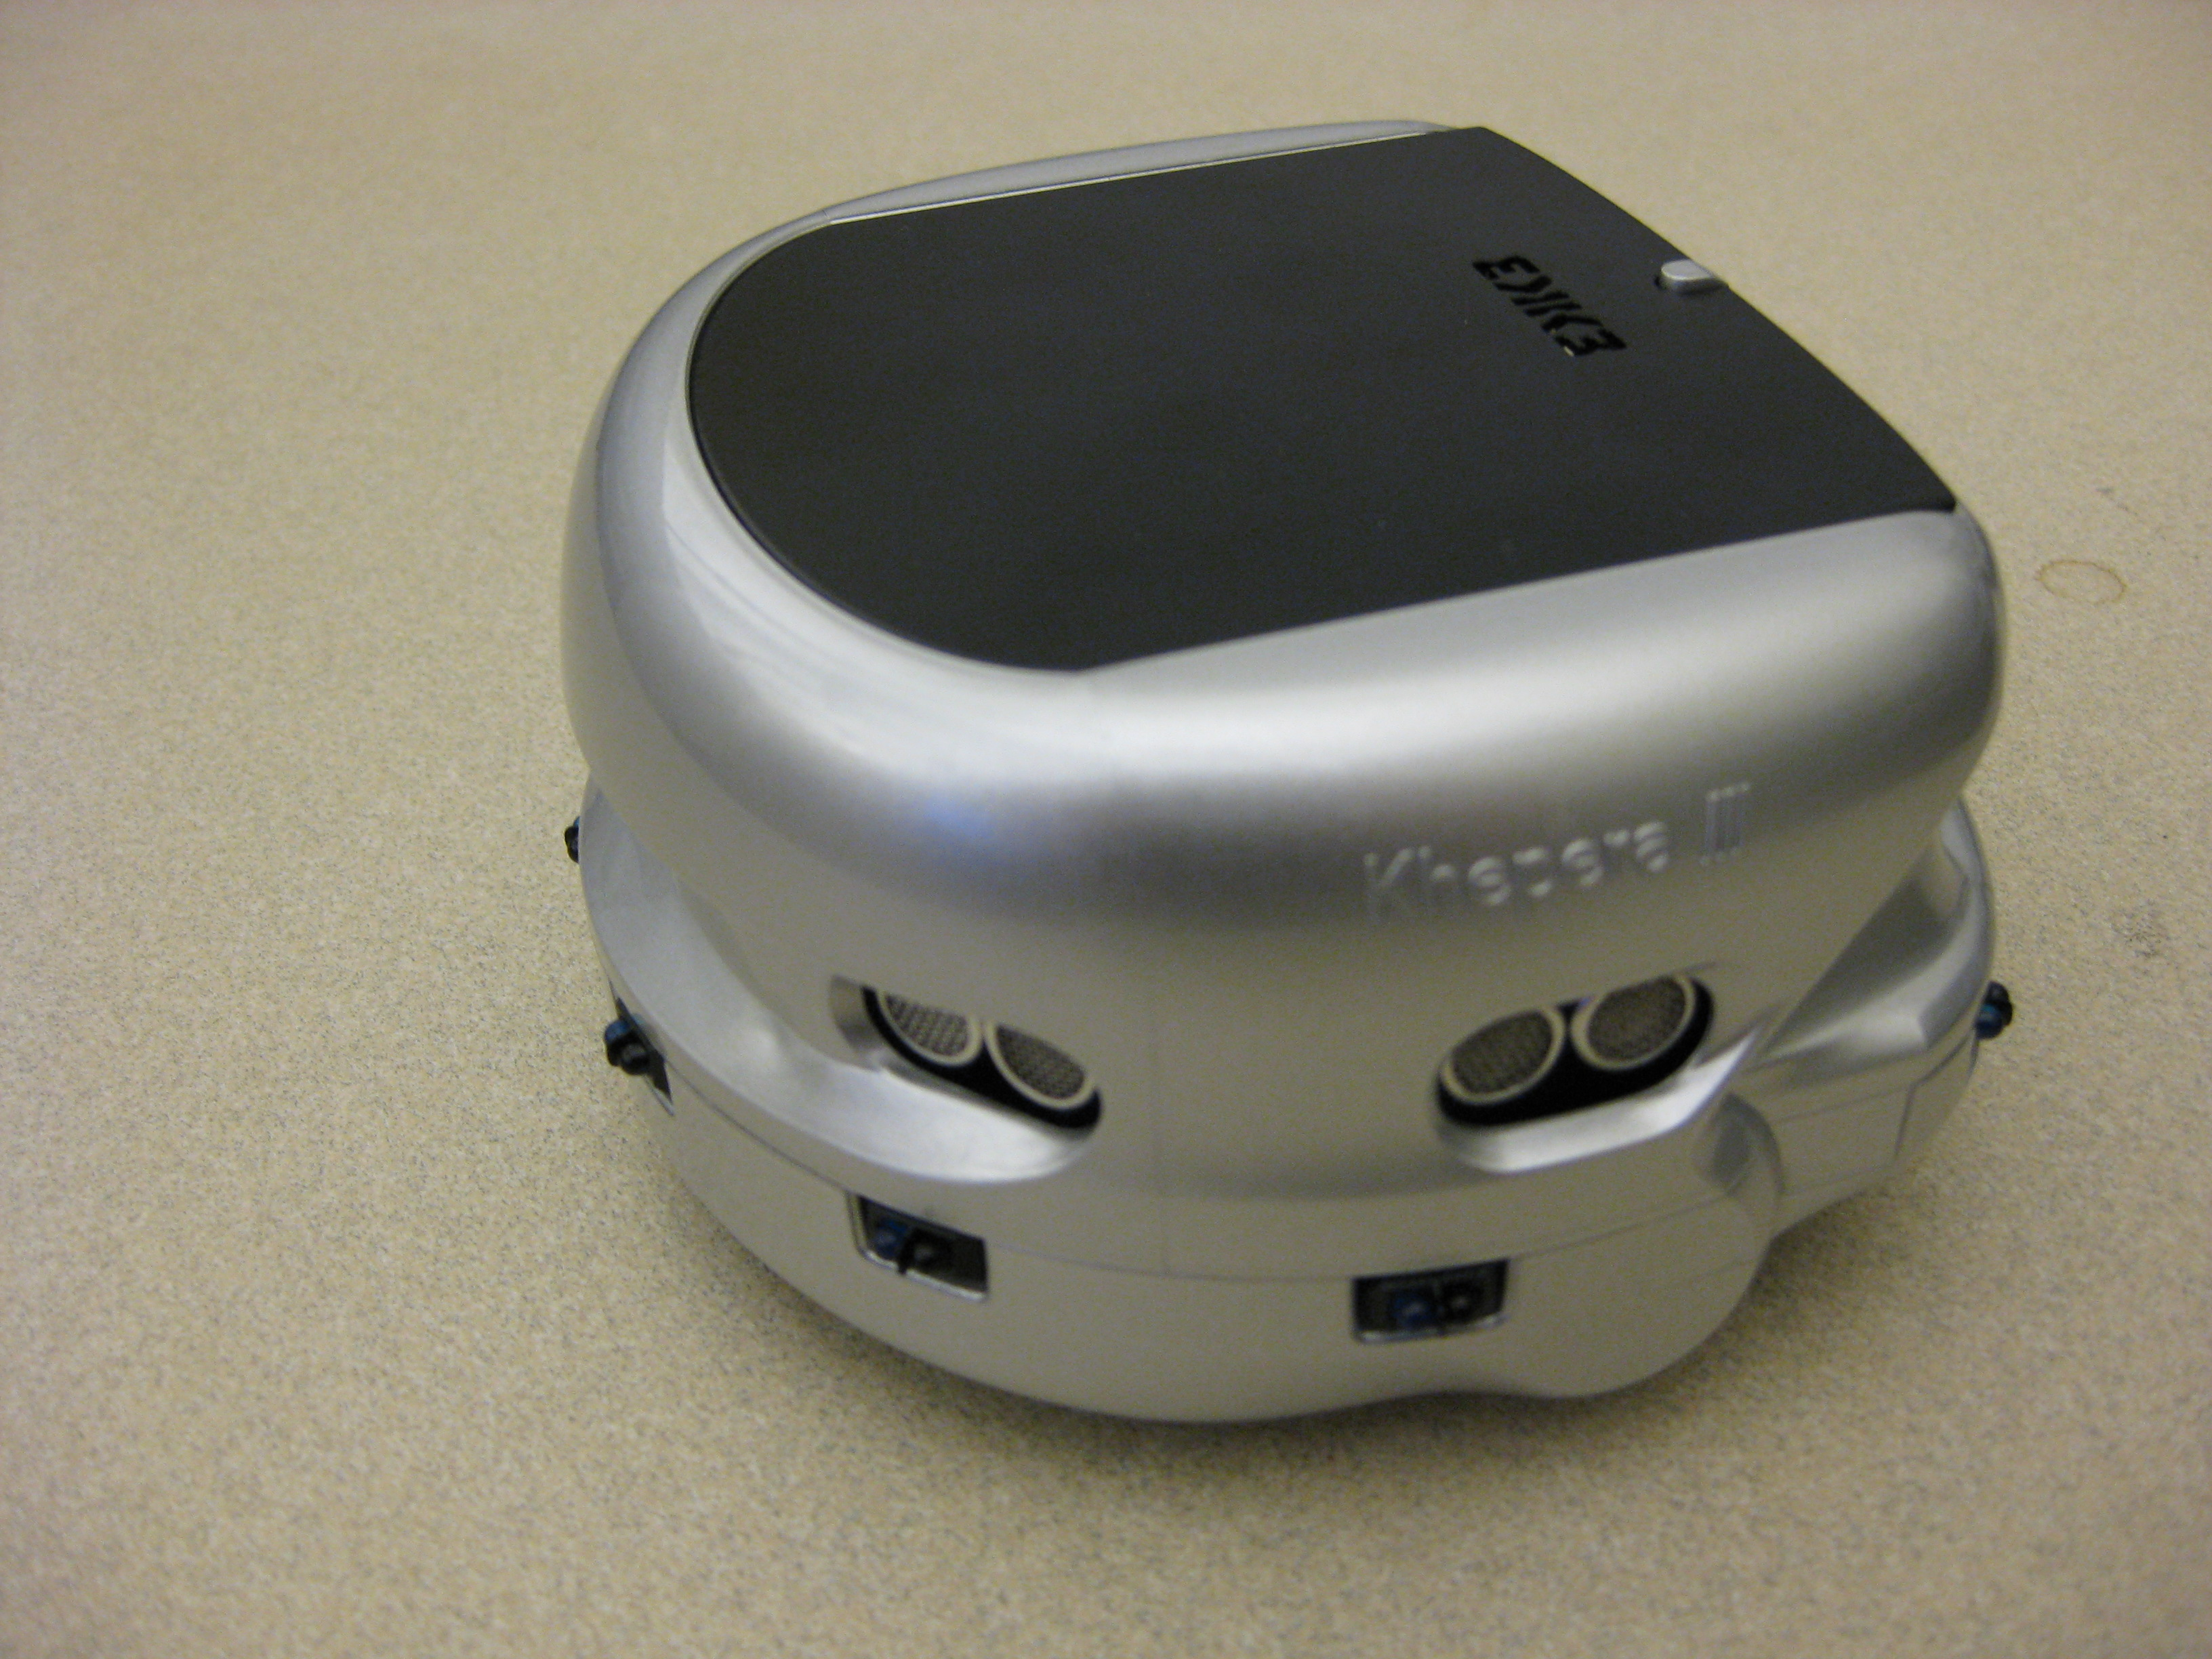
\includegraphics[trim= 8cm 0cm 0cm 0cm,clip,
scale=0.14]{Figuras/Khepera_III_robot}
		\subcaption{Robô Khepera 3}
	  	\label{fig:test1}
	\end{subfigure}
	~
	\begin{subfigure}[b]{0.49\textwidth}%
		\centering
		% fbox{}
		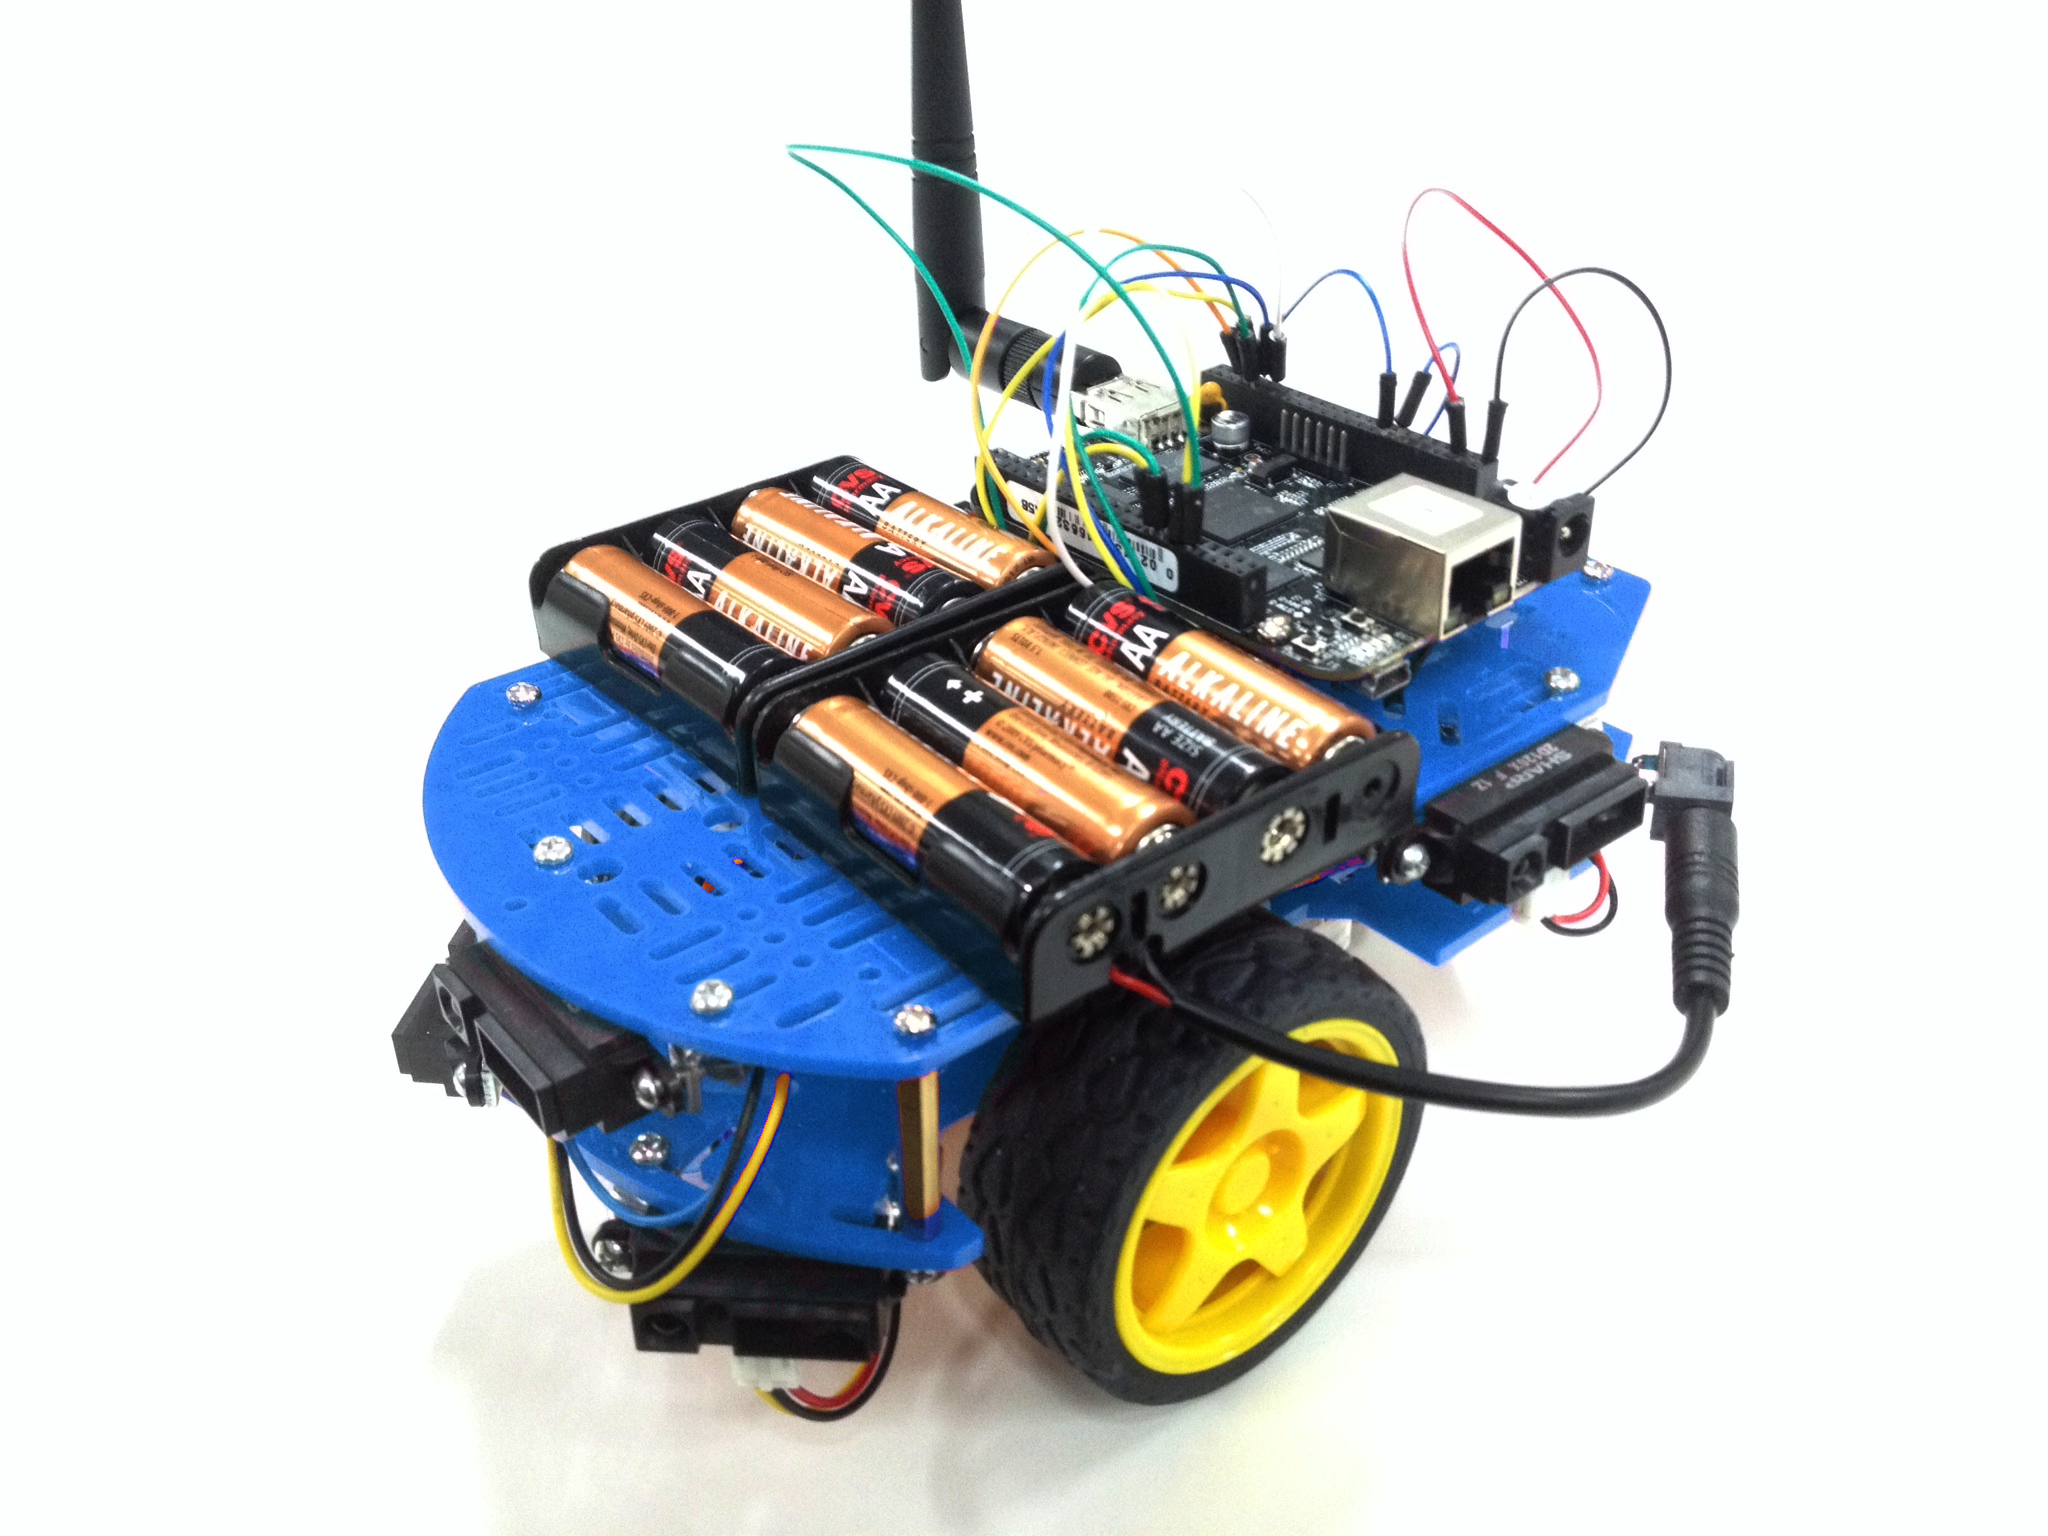
\includegraphics[trim={6cm 0cm 3cm 0cm},clip,
scale=0.09]{Figuras/quickbot-blue}
		\subcaption{Robô QuickBot}
	  	\label{fig:test2}
	\end{subfigure}
	
	\textbf{Fonte: \citeonline{im:Khepera}, \citeonline{im:QuickBot_Blue}}
\end{figure}


%		\begin{figure}[!htb]
%			\centering
%			\caption{Robôs Khepera e QuickBot fisicamente e em simulação}
%			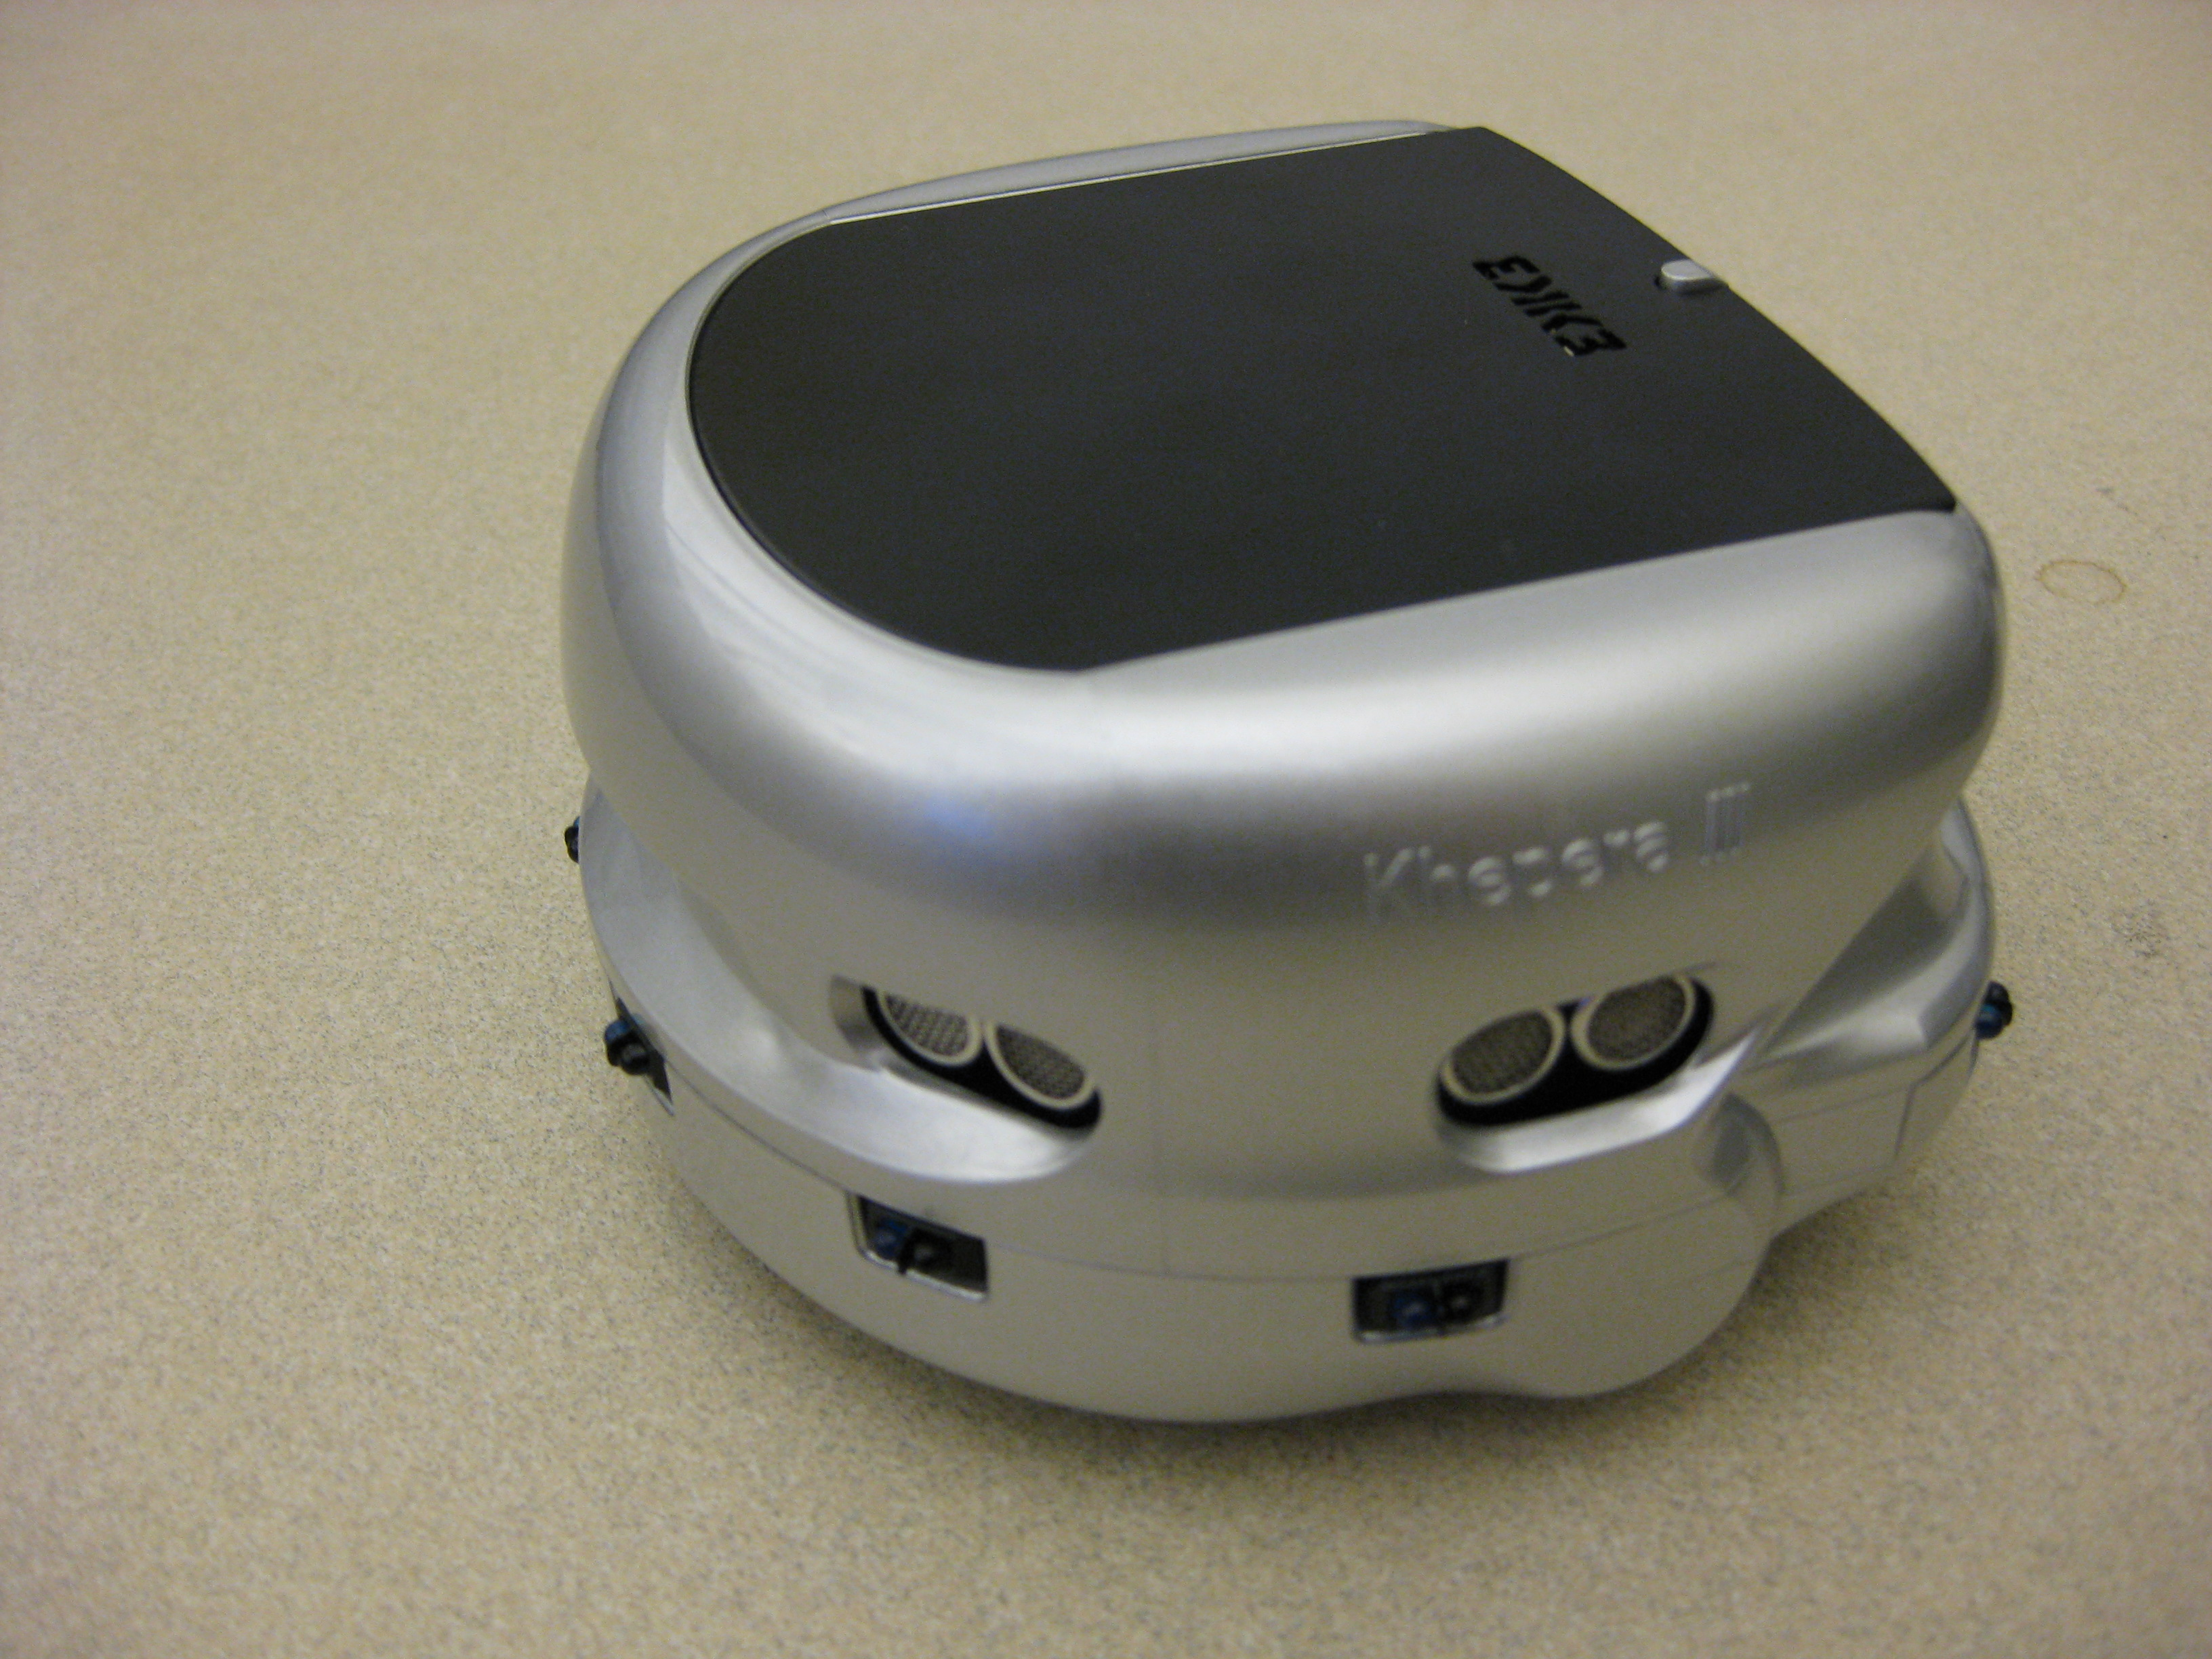
\includegraphics[trim={0cm 0cm 0cm 0cm},clip,
%scale=0.35]{Figuras/Khepera_III_robot}
%			%\vspace{-0.4cm}
%			\label{fig:RobosESim}
%		\end{figure}

%		\begin{figure}[!htb]
%			\centering			
%			\caption{Robôs Khepera e QuickBot fisicamente e em simulação}
%			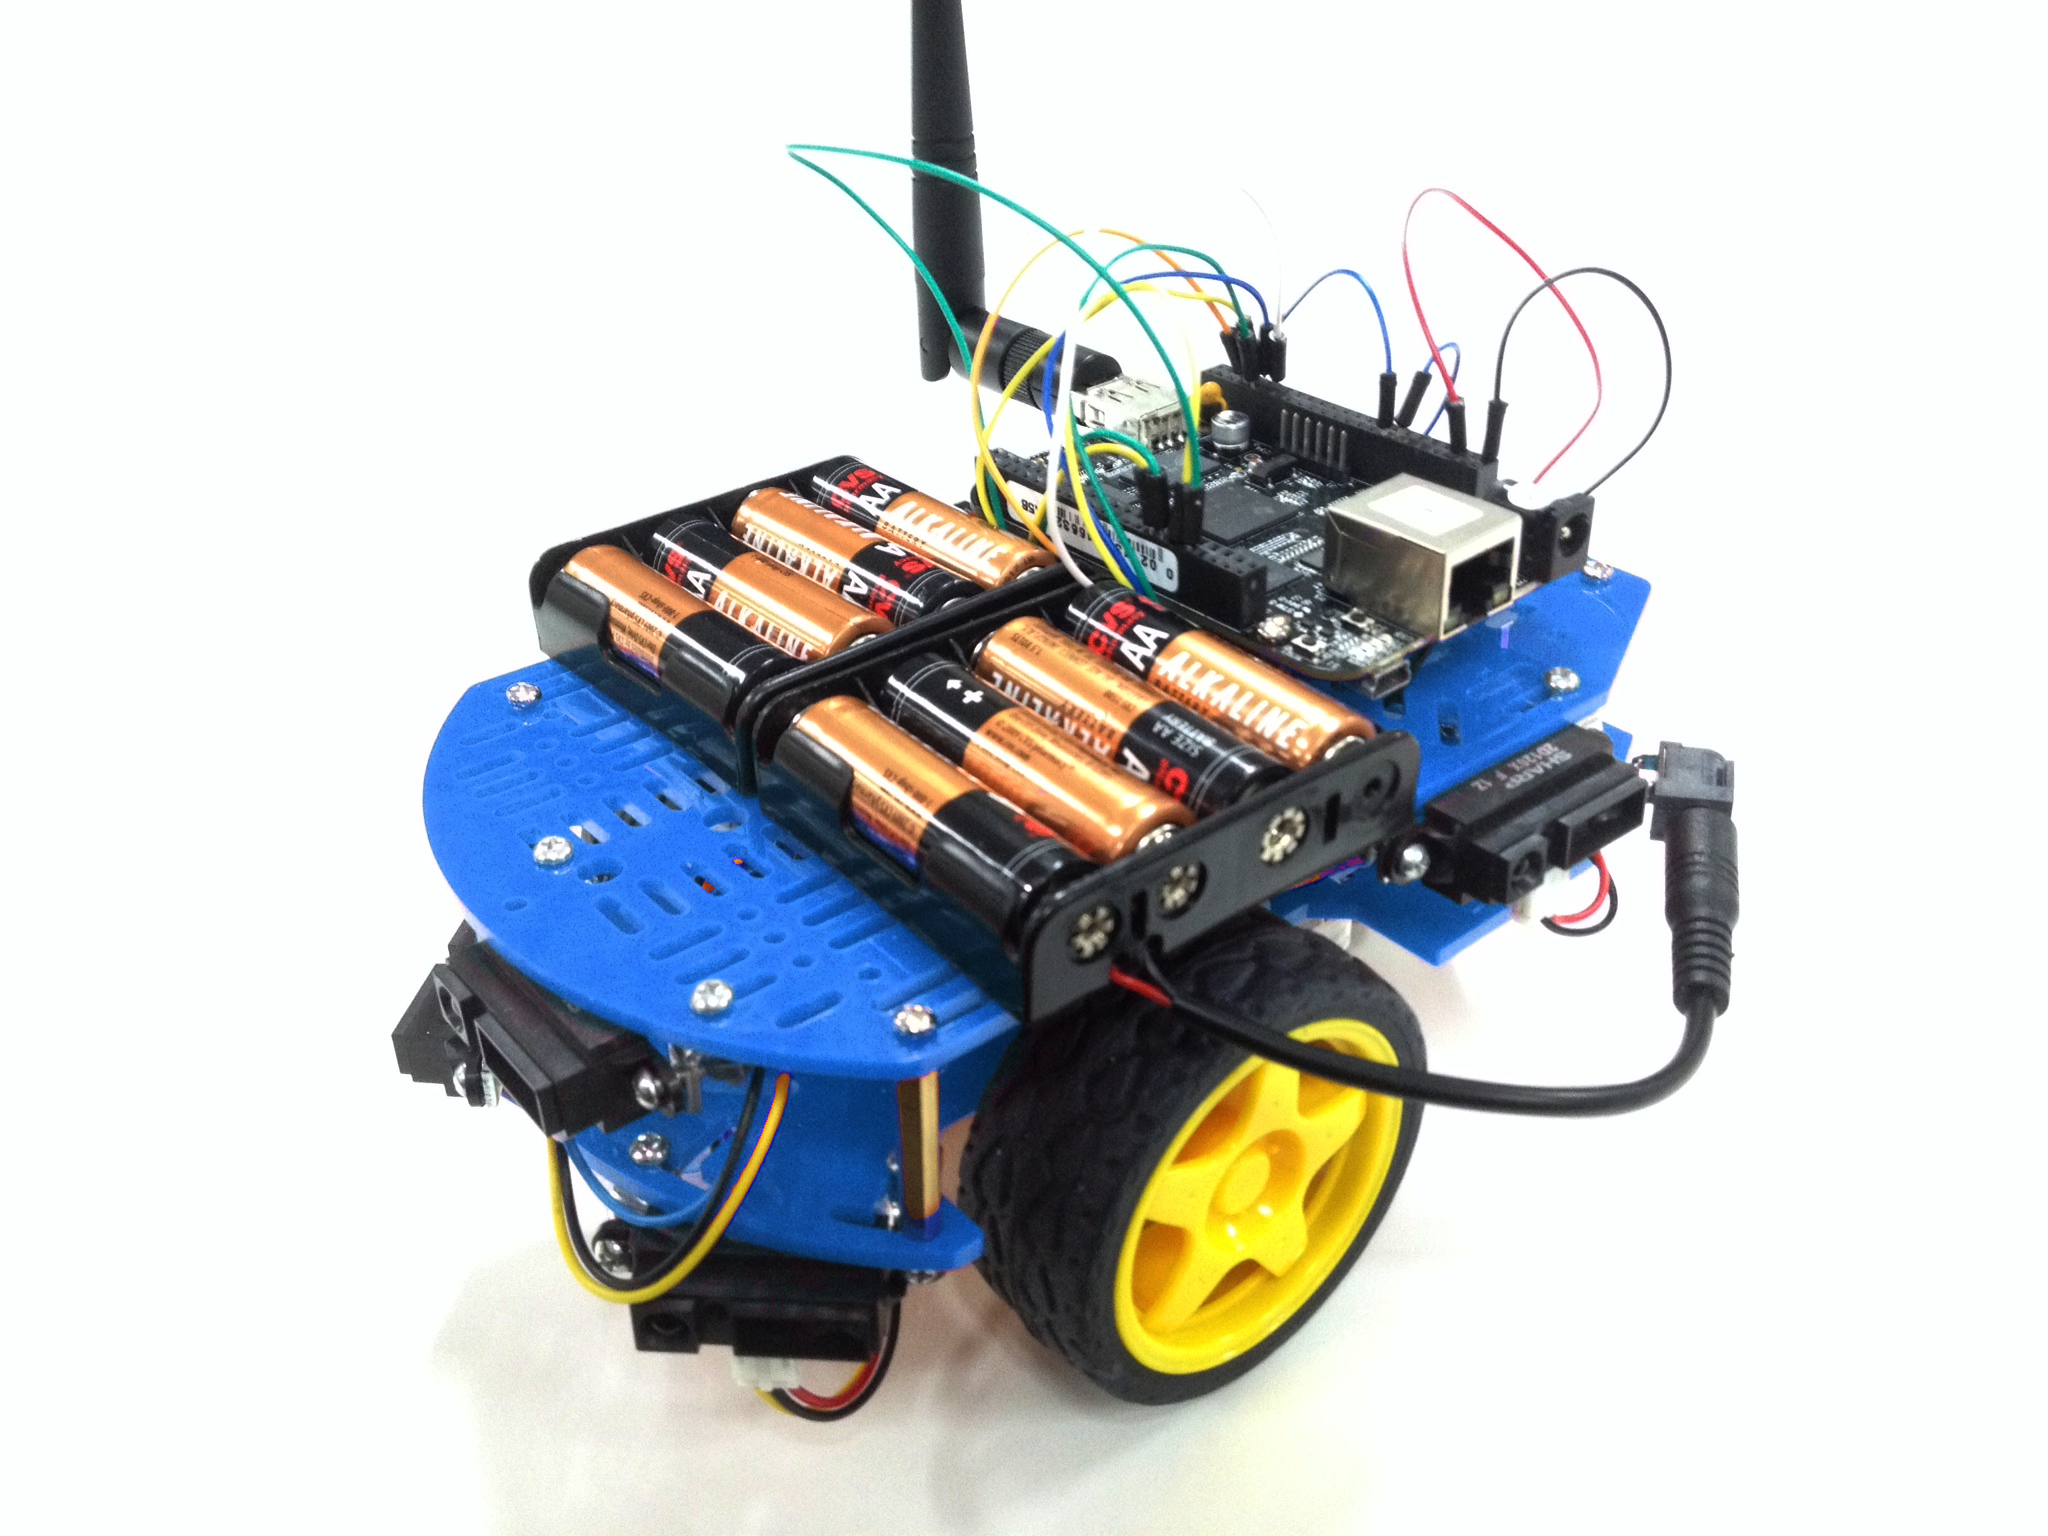
\includegraphics[trim={0cm 0cm 0cm 0cm},clip,
%scale=0.25]{Figuras/quickbot-blue}
%			%\vspace{-0.4cm}
%			\label{fig:RobosESim}
%		\end{figure}

%		\begin{figure}[!htb]
%			\centering
%			\caption{Robôs Khepera e QuickBot fisicamente e em simulação}
%			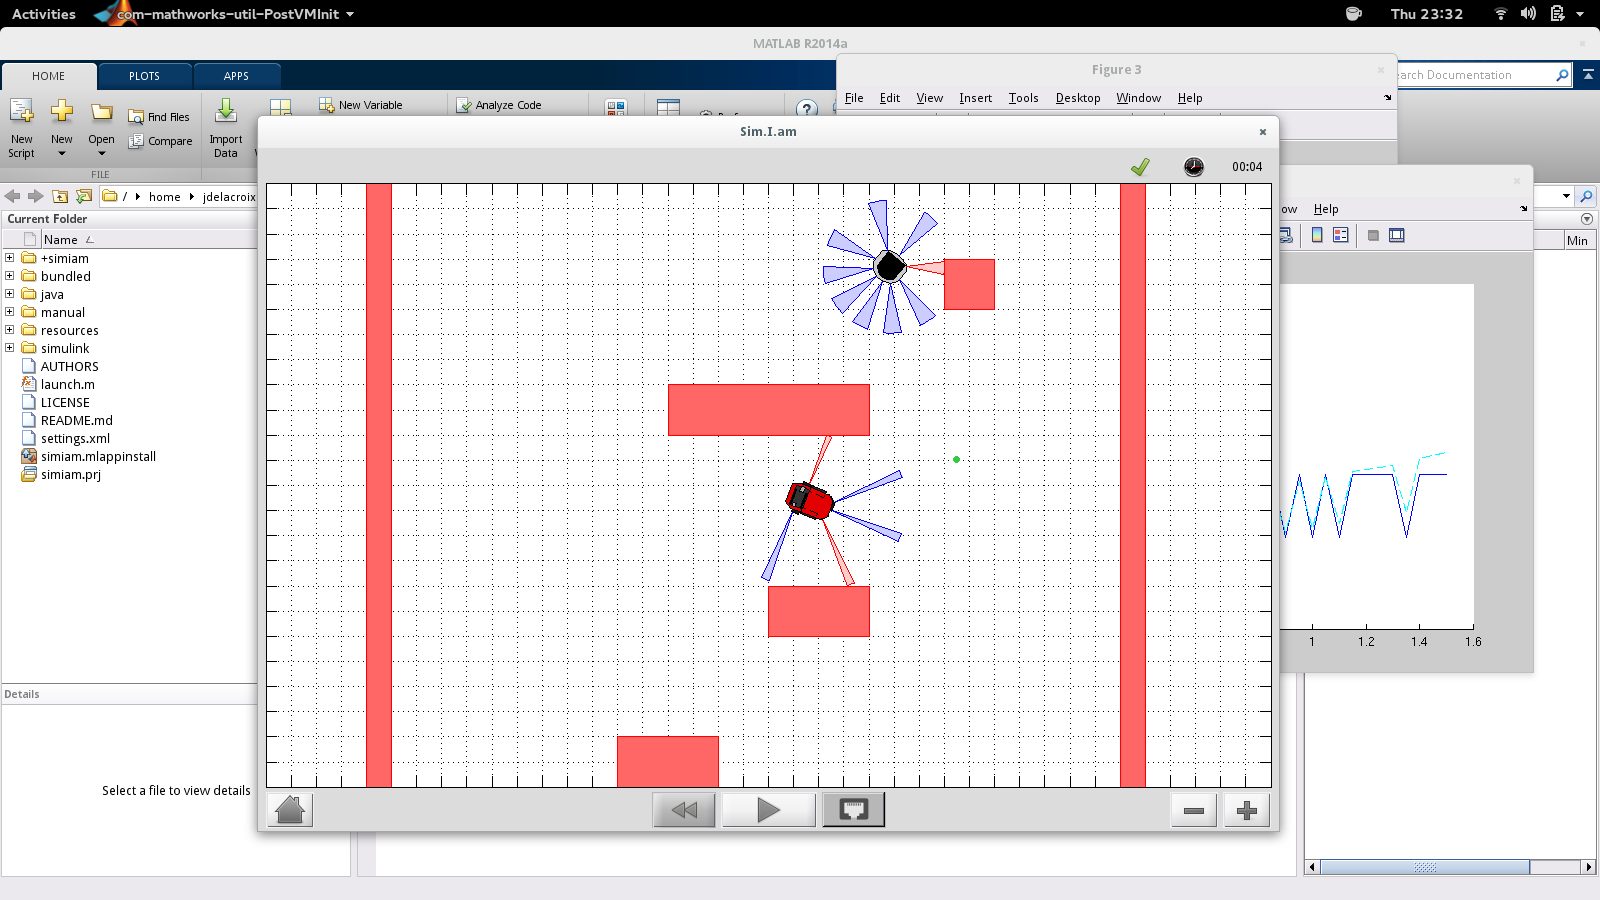
\includegraphics[trim={0cm 0cm 0cm 0cm},clip,
%scale=0.25]{Figuras/simiam-screenshot}
%			%\vspace{-0.4cm}
%			\label{fig:RobosESim}
%		\end{figure}


%\begin{figure}
%\begin{minipage}[c][11cm][t]{.5\textwidth}
%  \vspace*{\fill}
%  \centering
%  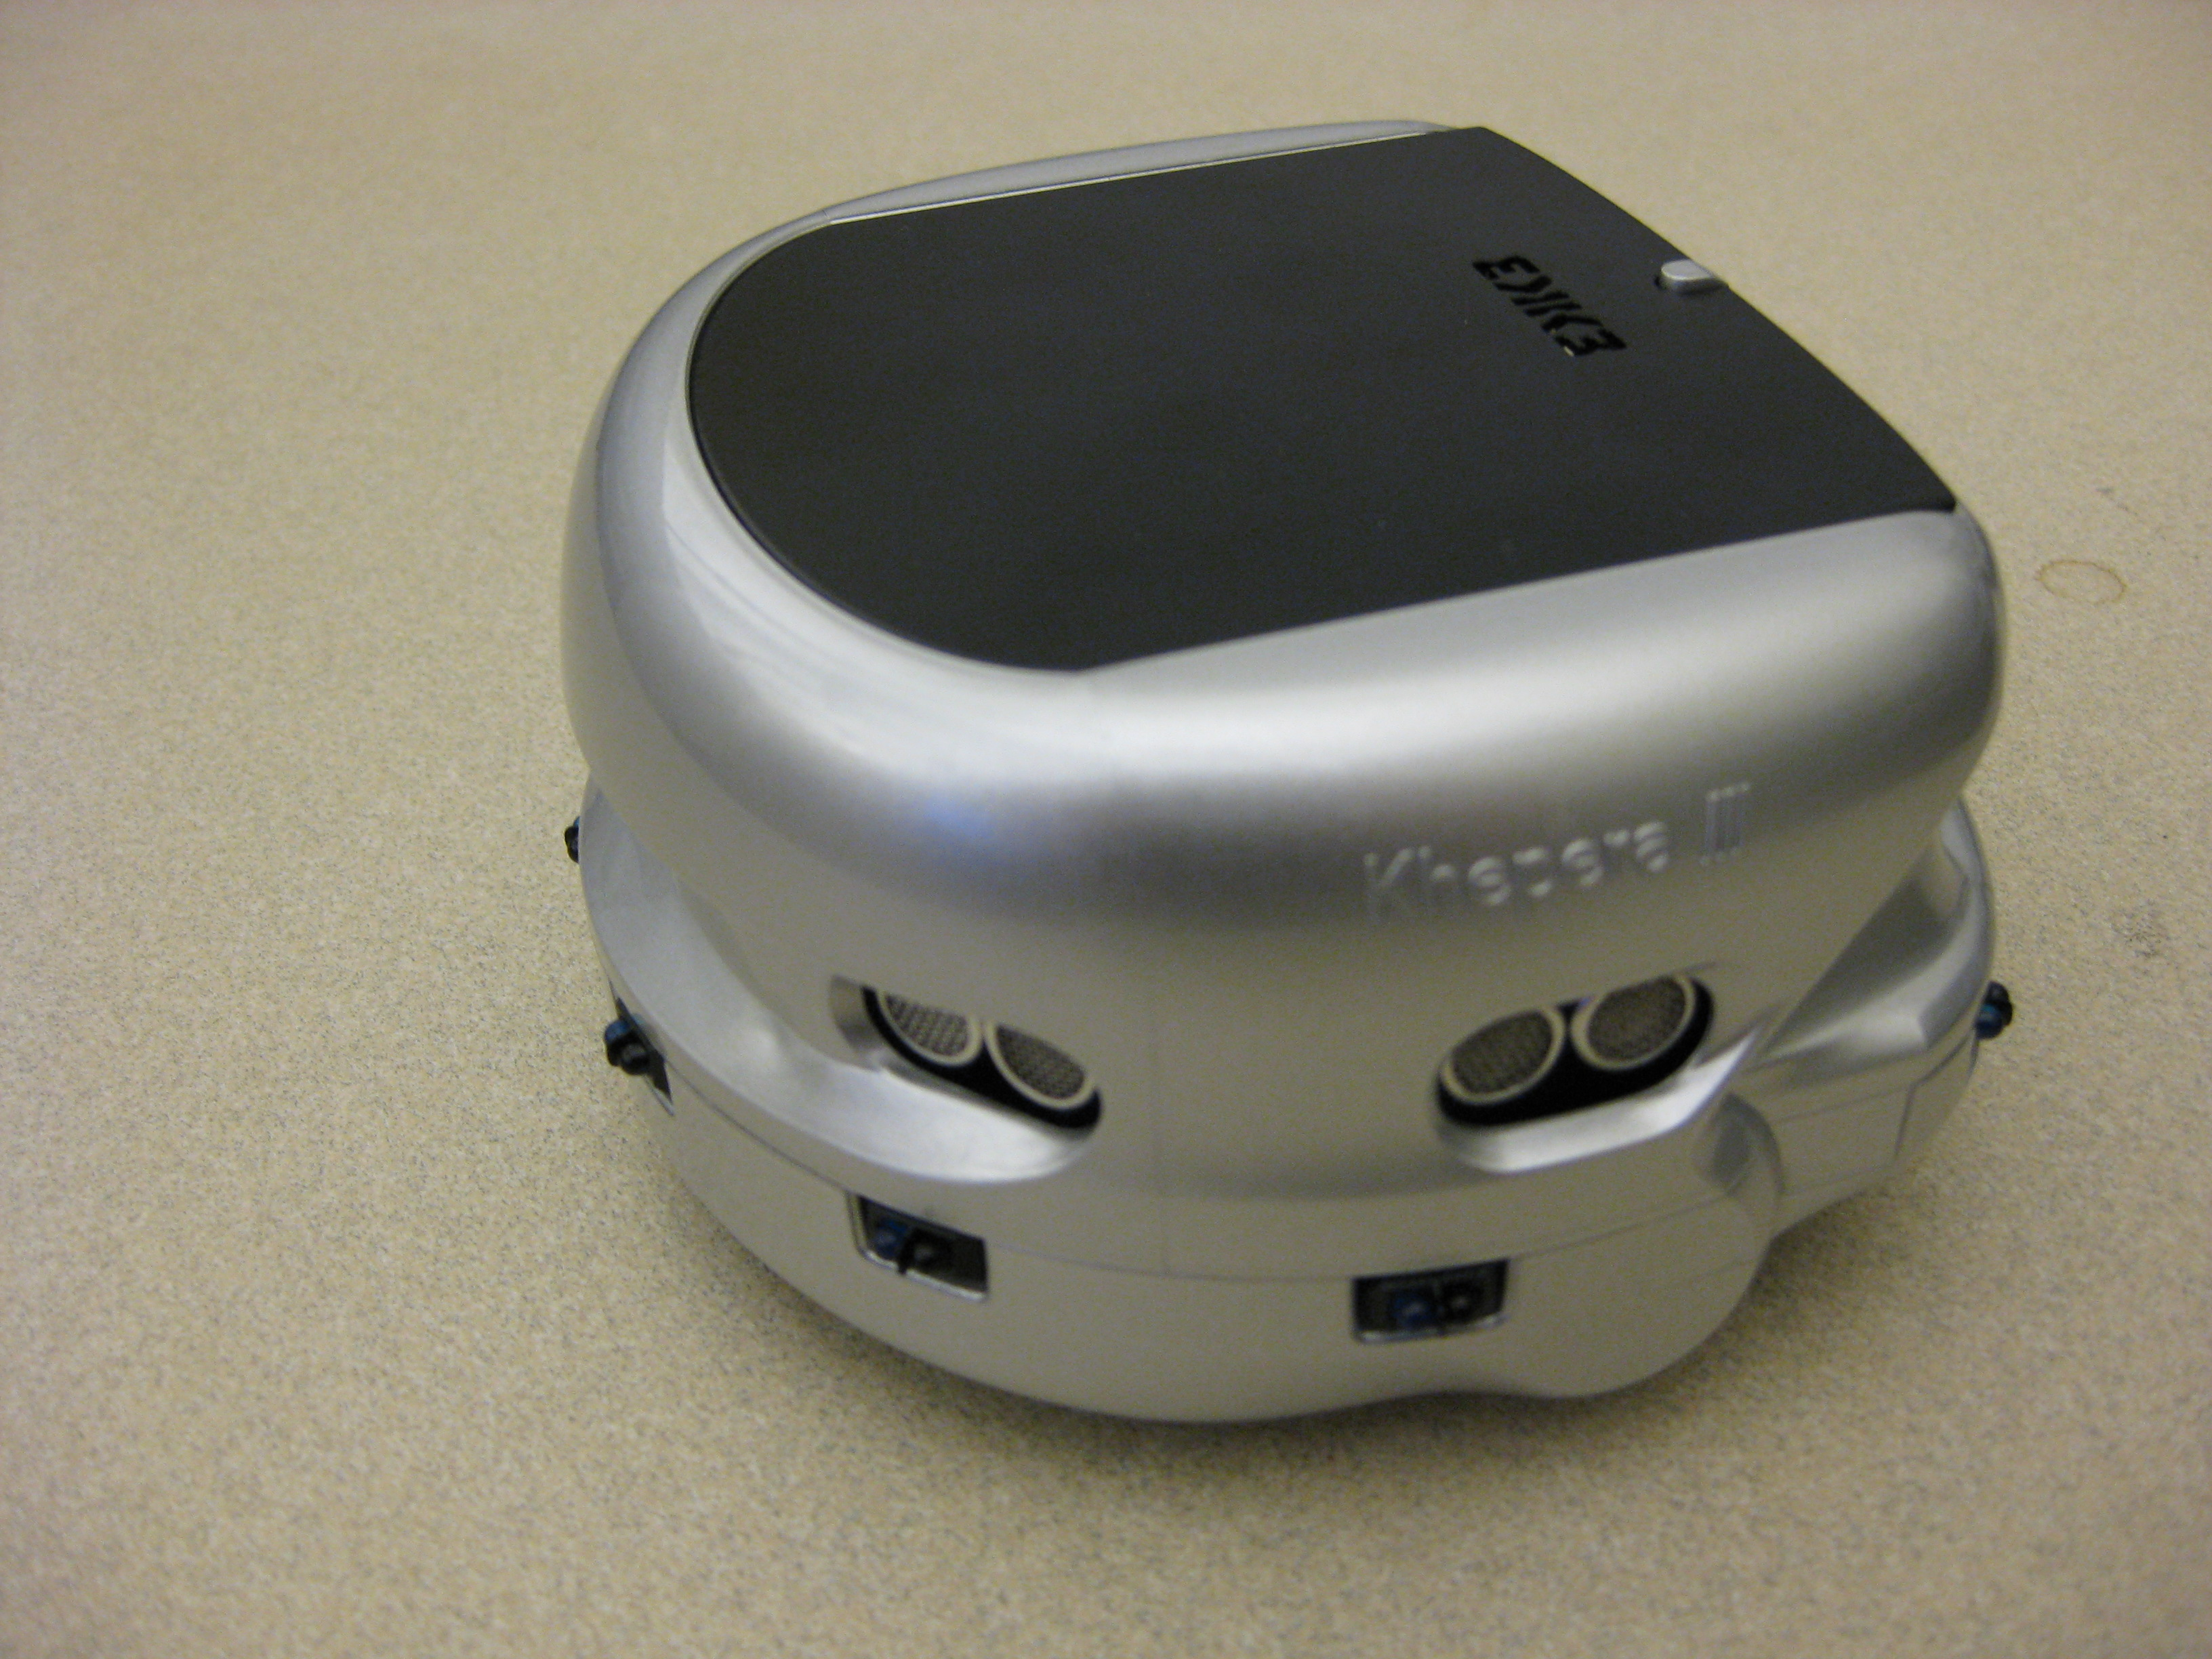
\includegraphics[width=5cm,height=4.5cm]{Figuras/Khepera_III_robot}
%  \subcaption{Robô Khepera}
%  \label{fig:test2}\par\vfill
%  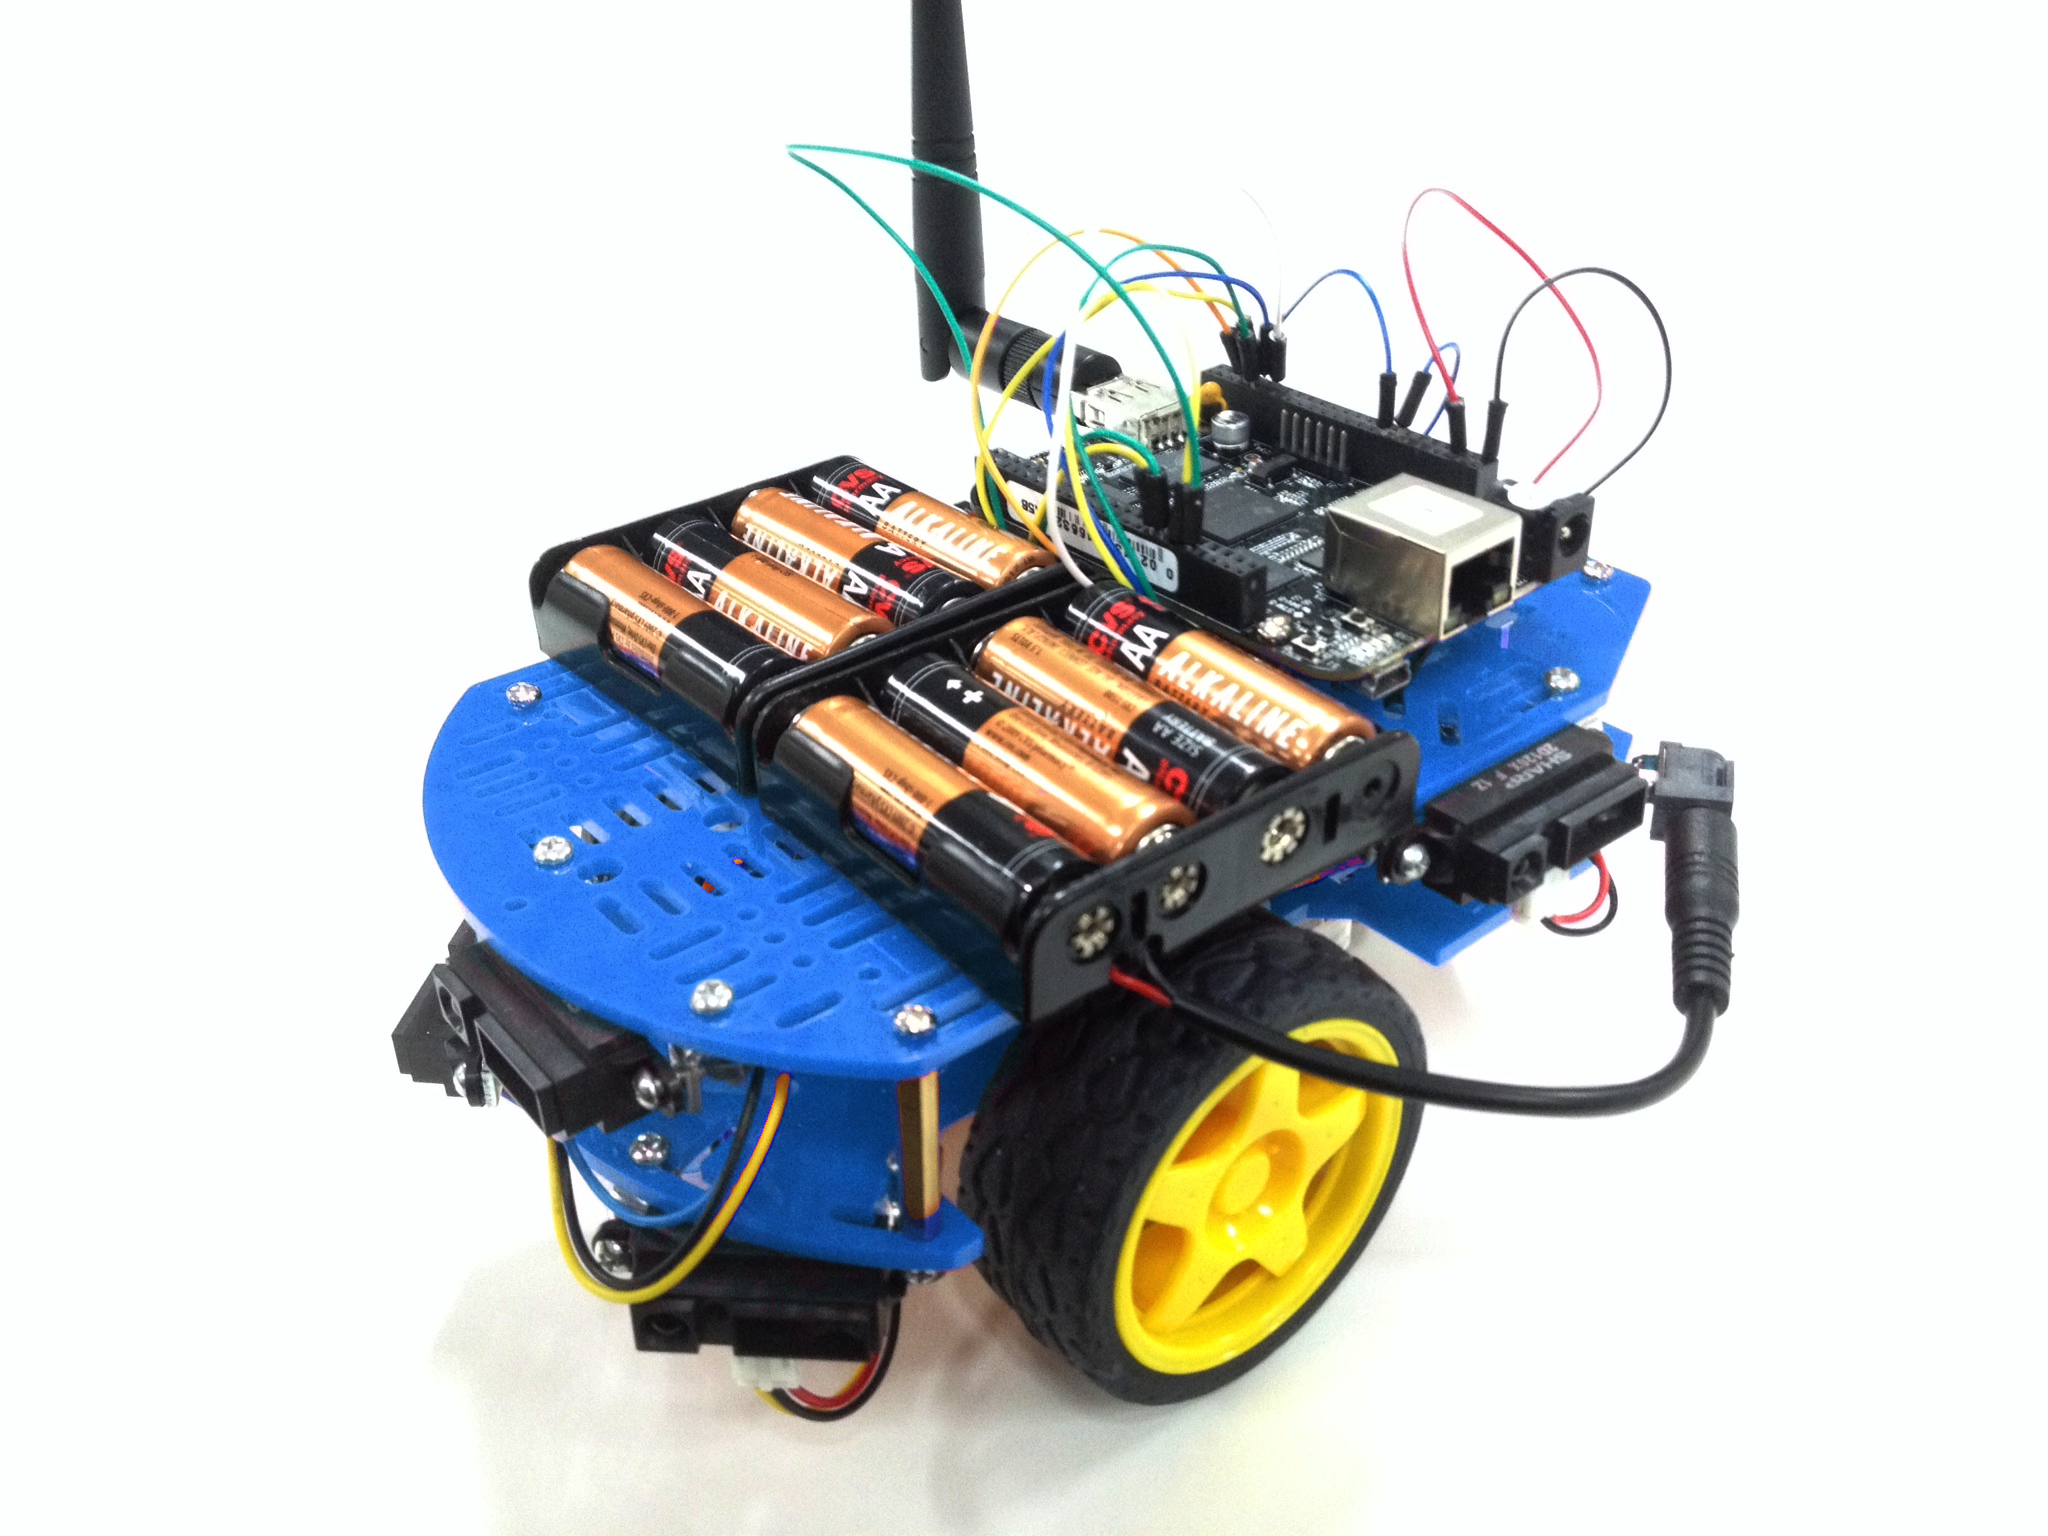
\includegraphics[width=5cm,height=4.5cm]{Figuras/quickbot-blue}
%  \subcaption{Robô QuickBot}
%  \label{fig:test3}
%\end{minipage}
%\begin{minipage}[c][11cm][t]{.5\textwidth}
%  \vspace*{\fill}
%  \centering
%  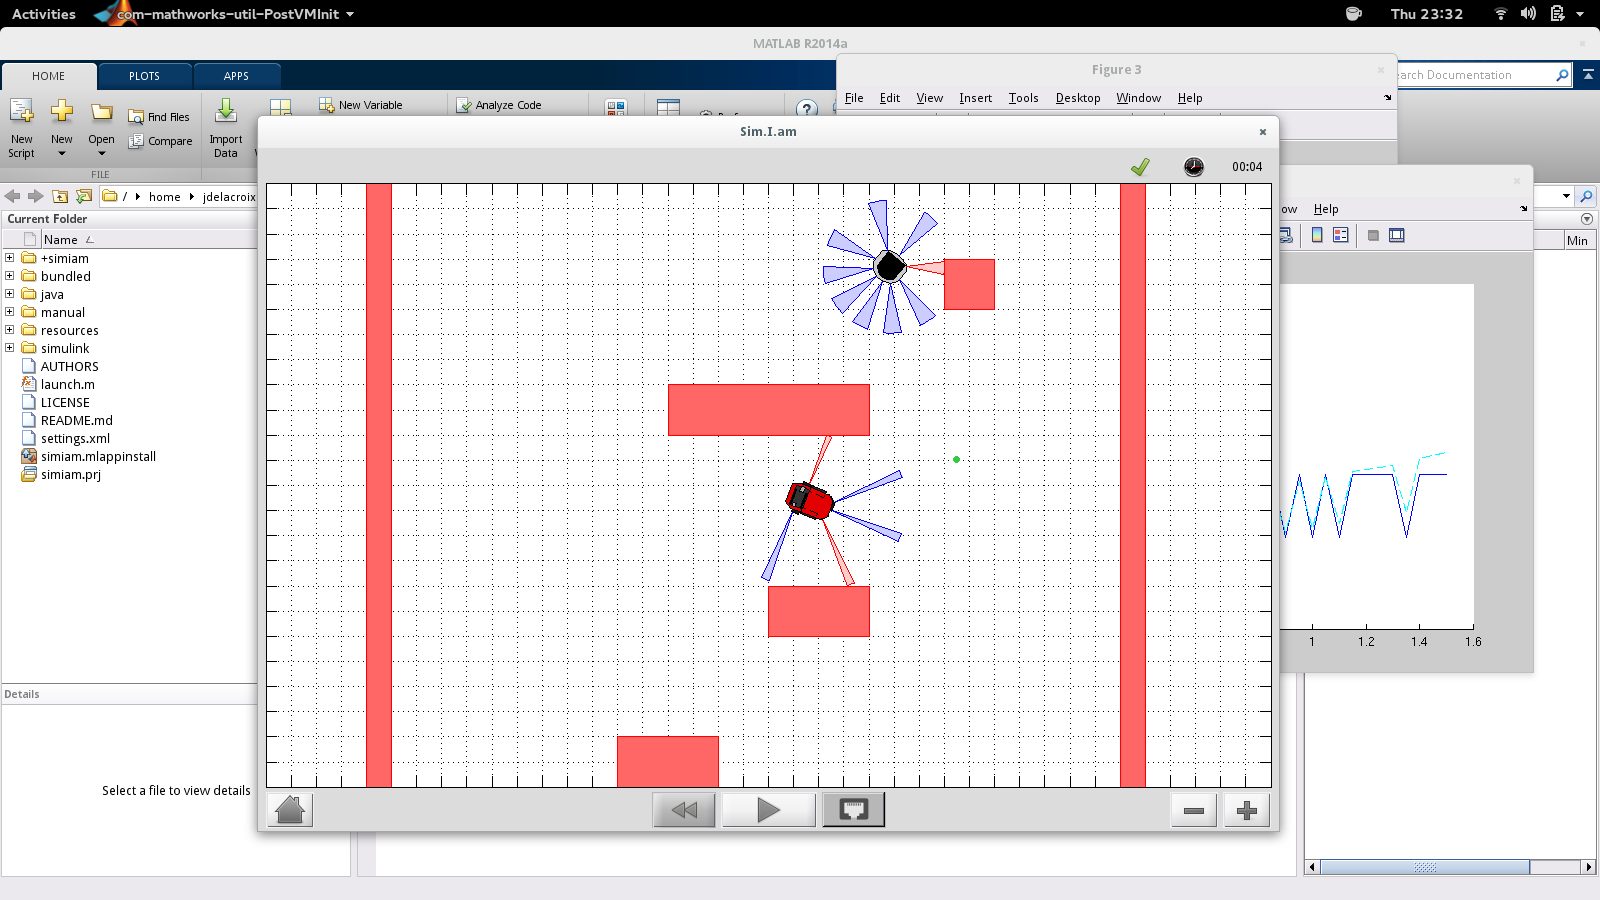
\includegraphics[width=5cm,height=10cm]{Figuras/simiam-screenshot}
%  \subcaption{Simulador Simiam}
%  \label{fig:test1}
%\end{minipage}%
%\end{figure}

\begin{figure}[ht]
\centering
\caption{Robôs Khepera 3 e QuickBot em simulação}
\label{fig:RobosEmSimulador}
		\centering
		% fbox{}
		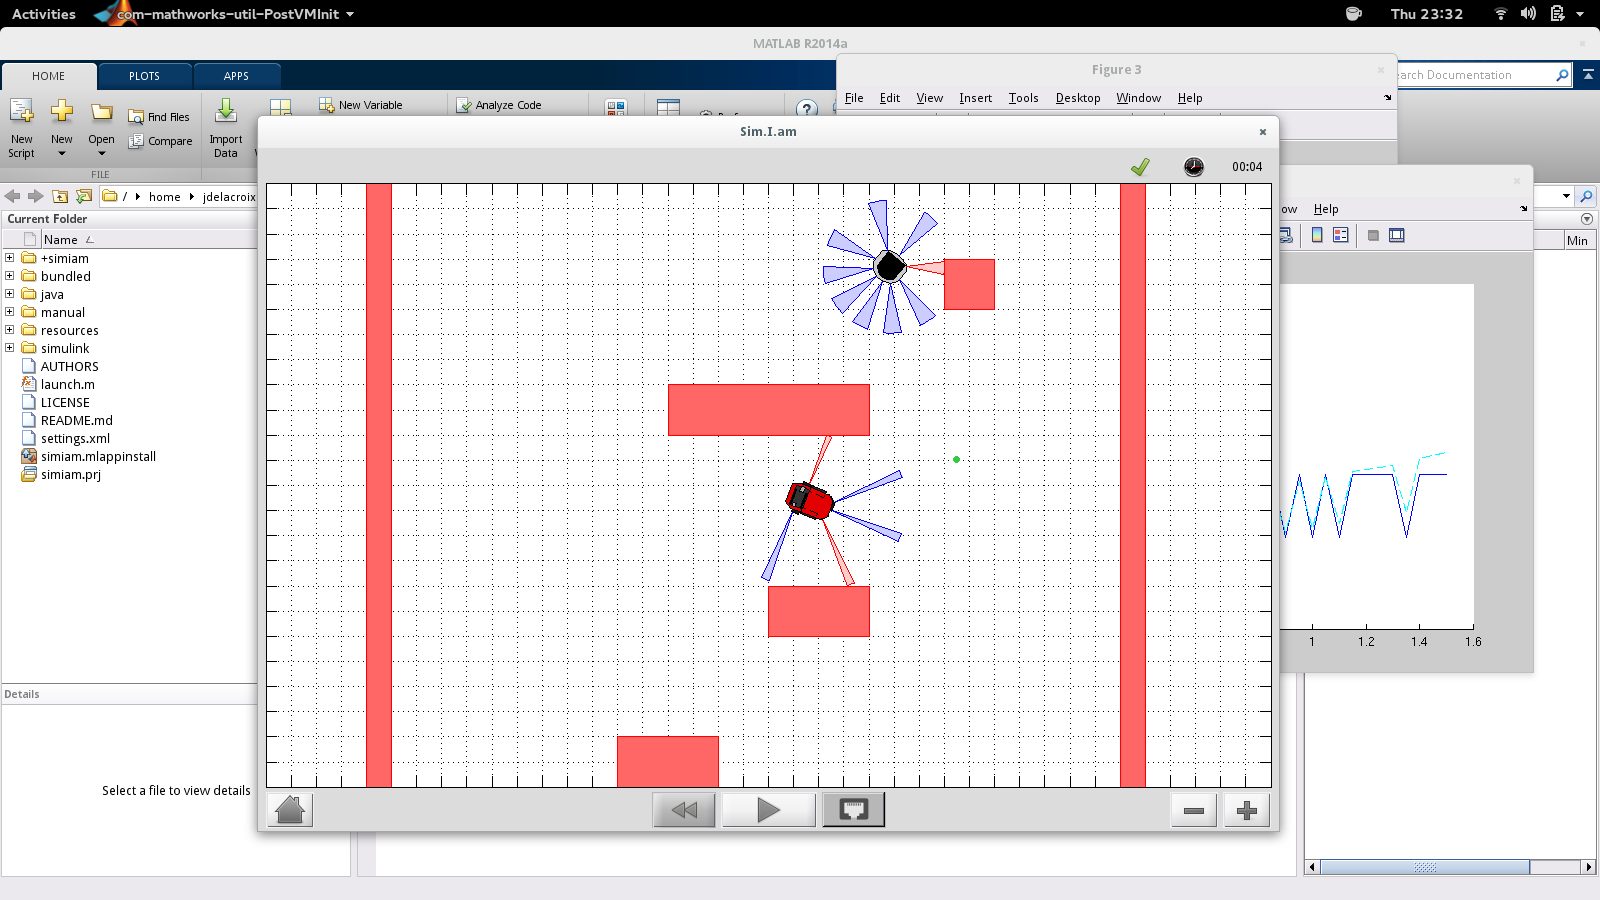
\includegraphics[trim={0cm 0cm 0cm 0cm},clip,
scale=0.24]{Figuras/simiam-screenshot}
	
	\textbf{Fonte: \citeonline{im:Simiam}}
\end{figure}

O Simiam é implementado como um aplicativo Matlab. Possui uma interface
gráfica intuitiva e uma arquitetura interna simples, facilmente customizável. As
subseções a seguir apresentam os pacotes mais importantes, bem como as
principais classes que os compõem e chama atenção para as alterações necessárias
a fim de tornar a simulação coerente com o presente trabalho.

	\subsubsection{Pacote ``ui''}
	
	O pacote ``ui'' é responsável pela interface gráfica do simulador. A classe
	``AppWindow'' possui um método construtor que inicializa atributos e o
	método ``load\_ui'' que invoca o método ``create\_layout", responsável por
	criar o leiaute da interface.
	
	O botão start, criado pelo método anterior é tratado por ``ui\_button\_start".
	Esta é a função principal reponsável por criar o ambiente de simulação
	(definido no arquivo ``settings.xml''), inserir um ou mais robôs e iniciar a
	simulação.
	
	Alterações mínimas foram efetuadas nesta etapa. Foram adicionados comandos para
	maximizar a janela do simulador e para ajustar o ``zoom'' de modo a permitir uma
	visão panorâmica de todo o ambiente de simulação. O arquivo de configuração
	``settings.xml'' foi alterado a fim de ajustar o ``tamanho do mundo'' ao
	tamanho da	tela.
	
	\subsubsection{Pacote ``simulator''}
	
	O pacote ``simulator'' realiza de fato a simulação. A classe ``World'' é
	responsável por extrair informações do arquivo ``.xml'', como quantidade e
	localização inicial de robôs e obstáculos, armazenado em estruturas de dados.
	A classe ``Simulator'' atualiza a simulação na janela, enquanto a
	classe ``Physics'' é responsável por detectar colisões de robôs com obstáculos
	e entre si. 
	
	As alterações neste pacote foram todas na classe ``Simulator'', no intuito
	de possibilitar a captura da simulação em video ``.mp4" ou ``.gif". Apesar de
	não ser uma alteração fundamental para a etapa de execução do trabalho, é
	necessária para a apresentação. Não foi criado um botão na interface para
	especificar ao simulador a captura em video. Assim, é necessário, no
	construtor da classe Simulator, atribuir valor verdadeiro aos atributos
	``gravarvideo'' e/ou ``gravargif". 
	
	\subsubsection{Pacote ``robot''}
	
	O pacote ``robot'' define um ou mais robôs passíveis de serem instanciados. A
	classe ``QuickBot'' estabelece parâmetros físicos, tais como informações
	geométricas, posicionamento dos sensores no corpo do robô e estabelece
	limitações, como velocidades de saturação e zona morta dos motores. Além de
	instanciar objetos das classes ``DifferentialDrive'', ``ProximitySensor'' e
	``WheelEncoder'', ``QuickBot'' extende a classe ``Robot''. 
	
	A classe ``DifferentialDrive" implementa a ``dinâmica'' dos modelos de
	acionamento diferencial e uniciclo. Com os métodos ``uni\_to\_diff'' e ``diff\_to\_uni'', a
	equivalência com o modelo apresentado na Equação \ref{eq:vw_to_diff} é
	estabelecida no espaço de simulação. 

	A classe ``ProximitySensor'' estabelece características do sensor infravermelho
	usado no QuickBot, tais como distâncias mínimas e máximas, espalhamento, localização e
	direção em relação ao corpo do robô e adiciona um ruído gaussiano.
	``WheelEncoder'', similarmente, estabelece características do \textit{encoder}.
	
	As alterações nesta etapa foram no intuito de incluir o robô deste trabalho
	no Simiam. O arquivo ``settings.xml'' deve determinar que um objeto (robô) da
	nova classe criada seja instanciado, ao invés do objeto da classe QuickBot.
	
	\subsubsection{Pacote ``controller''}
	
	O pacote ``controller'' é responsável pela implementação de todos os
	controladores e supervisores dos robôs implementados. A classe ``Supervisor'' é
	extendida para obter o controlador supervisório de cada robô a ser simulado.
	Para o QuickBot e Khepera 3, os respectivos supervisores são definidos pelas
	classes ``QBSupervisor'' e ``K3Supervisor''. Essas classes definem máquinas de
	estado, onde cada estado é associado a um controlador de variável contínua.
	Esses controladores, por sua vez, extendem a classe ``Controller'' e
	implementam os ``comportamentos'', ou modos, dos robôs.
	% Calculo de odometria está em QBSupervisor.
	
	As alterações neste pacote foram responsáveis pela inclusão de suporte a
	controladores \textit{Fuzzy}, além de adicionar o supervisório específico para
	o robô desenvolvido.

\subsection{Especificações}

As variáveis L e R na Equação \ref{eq:diff}, para o robô deste trabalho, valem
respectivamente 18 cm e 3,4 cm.

O robô deste trabalho foi feito com base no robô ``QuickBot''. Contudo, o sensor infravermelho do ``QuickBot''
é o ``GP2Y0A41SK0F'', cuja região de medição está no intervalo entre 4 e 30 cm. Por conta deste sensor estar 
obsoleto, ele foi substituído pelo ``GP2Y0A21YK0F'' que possui a curva de tensão por distância representada na 
Figura \ref{fig:SensorIR}. A faixa de distância do sensor deste trabalho está entre 10 e 80 cm, como pode ser visto
na Figura. 

\begin{figure}[ht]
	\centering
	\caption{Resposta do sensor infravermelho}
	\label{fig:SensorIR}
	
	%\fbox{}
	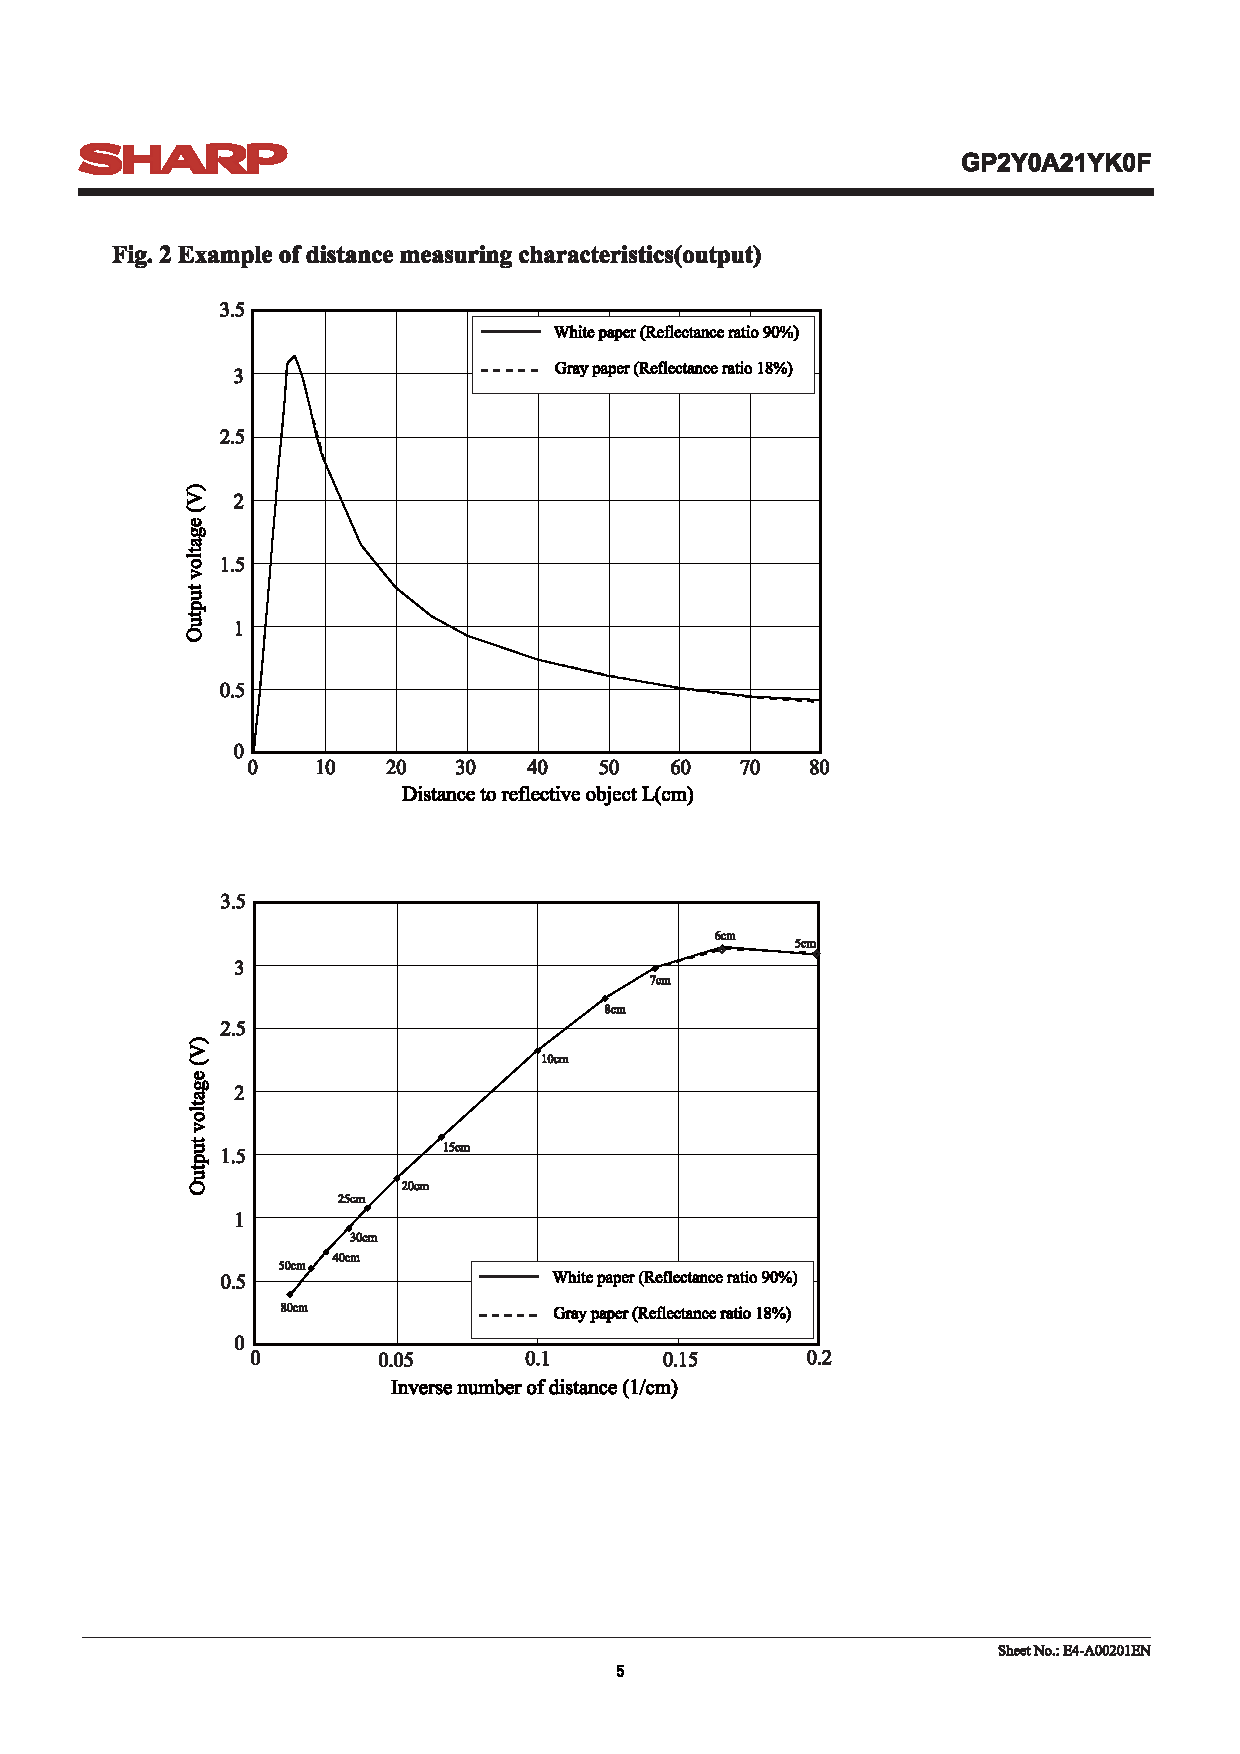
\includegraphics[trim= 3cm 15.8cm 6.5cm 4.8cm,clip,
scale=1]{Figuras/IR_Datasheet_Figure}

	%\begin{tikzpicture}[auto, node distance=2cm, on grid,
%>=latex']%
	
	%\node[anchor=south west,inner sep=0] (image) at (0,0) {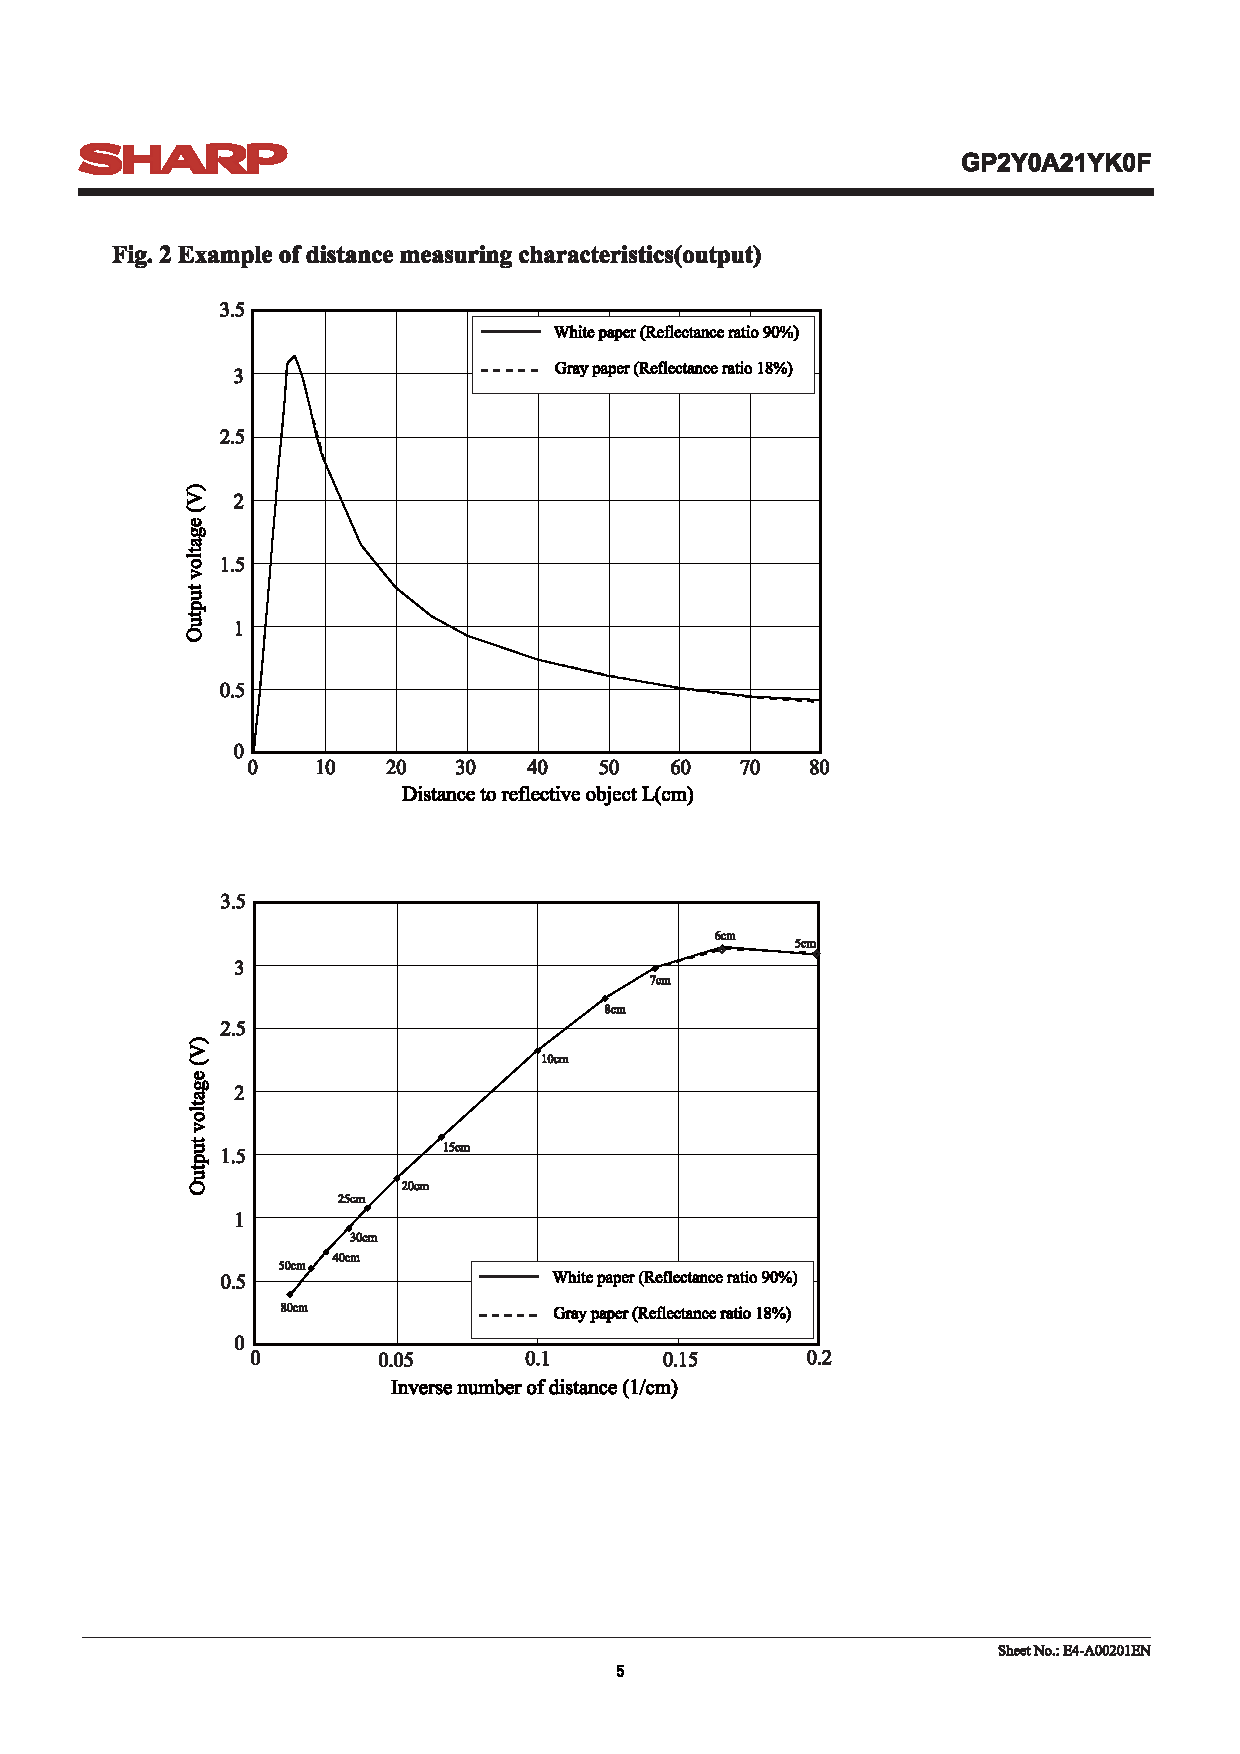
\includegraphics[trim =
%		{3cm 15.8cm 6.5cm 4.8cm}, clip,scale=1]{Figuras/IR_Datasheet_Figure}};
		
%	\node[fill,circle,inner sep=0.1pt, color = red] at (1.29,1.161) {};
%	\node[fill,circle,inner sep=0.1pt, color = red] at (2.525,2.235) {};
	
%	\node[fill,circle,inner sep=0.1pt, color = red] at (1.83,7.75) {};
	
	
%	\node[inner sep = 0 pt, outer sep = 0 pt] (origin) at (1.3,1.15) {};
%	\node[inner sep = 0 pt, outer sep = 0 pt] (teste2) at (2.55,2.25) {};
%	
%	\node[inner sep = 0 pt, outer sep = 0 pt] (P1) at (1.85,7.85) {};
	
	%\draw[-, color = red] (origin) -- (teste2);
	%\draw[-, color = red] (origin) -- (P1);
	
	%\node[] at (0,0) {};
	%\coordinate[] (teste1) {};
	%\coordinate[] (teste2) {};
	
	%\draw[-, color = red] (-18,2) -- (-7,3);
	
%	\end{tikzpicture}


	\textbf{Fonte: \citeonline{datasheet:SensorIR}}
\end{figure}

Para a região da curva onde $d > 4.95 cm$, o polinômio que a aproxima, associando
a distância pela tensão ($d(v)$), obtido utilizando a função ``polyfit'' do Matlab pode ser visto 
na Equação \ref{eq:PolinomioVx}.
\begin{equation}
	\label{eq:PolinomioVx}
	\begin{split}
		d(v) = 2.7802212625 v^6 -35.1150300110 v^5 + 179.6031433005 v^4 \\
		-477.9449116299 v^3 + 706.3400747125 v^2 -569.7367375002 v + 221.2678651473
	\end{split}
\end{equation}

\subsection{Montagem Física}

	Nesta seção pretende-se mostrar as questões práticas necessárias para a construção do 
	robô.
	
\subsubsection{Processo de montagem}

	Os componentes físicos do robô podem ser vistos na Figura \ref{fig:RoboReal}. Alguns
	números foram acrescentados às imagens ao lado dos periféricos utilizados, a fim de 
	rotulá-los.
	
	\begin{figure}[!ht]
\centering
\caption{Materiais e robô após montagem}
\label{fig:RoboReal}
	\begin{subfigure}[b]{0.49\textwidth}%
		\centering
		% fbox{}
		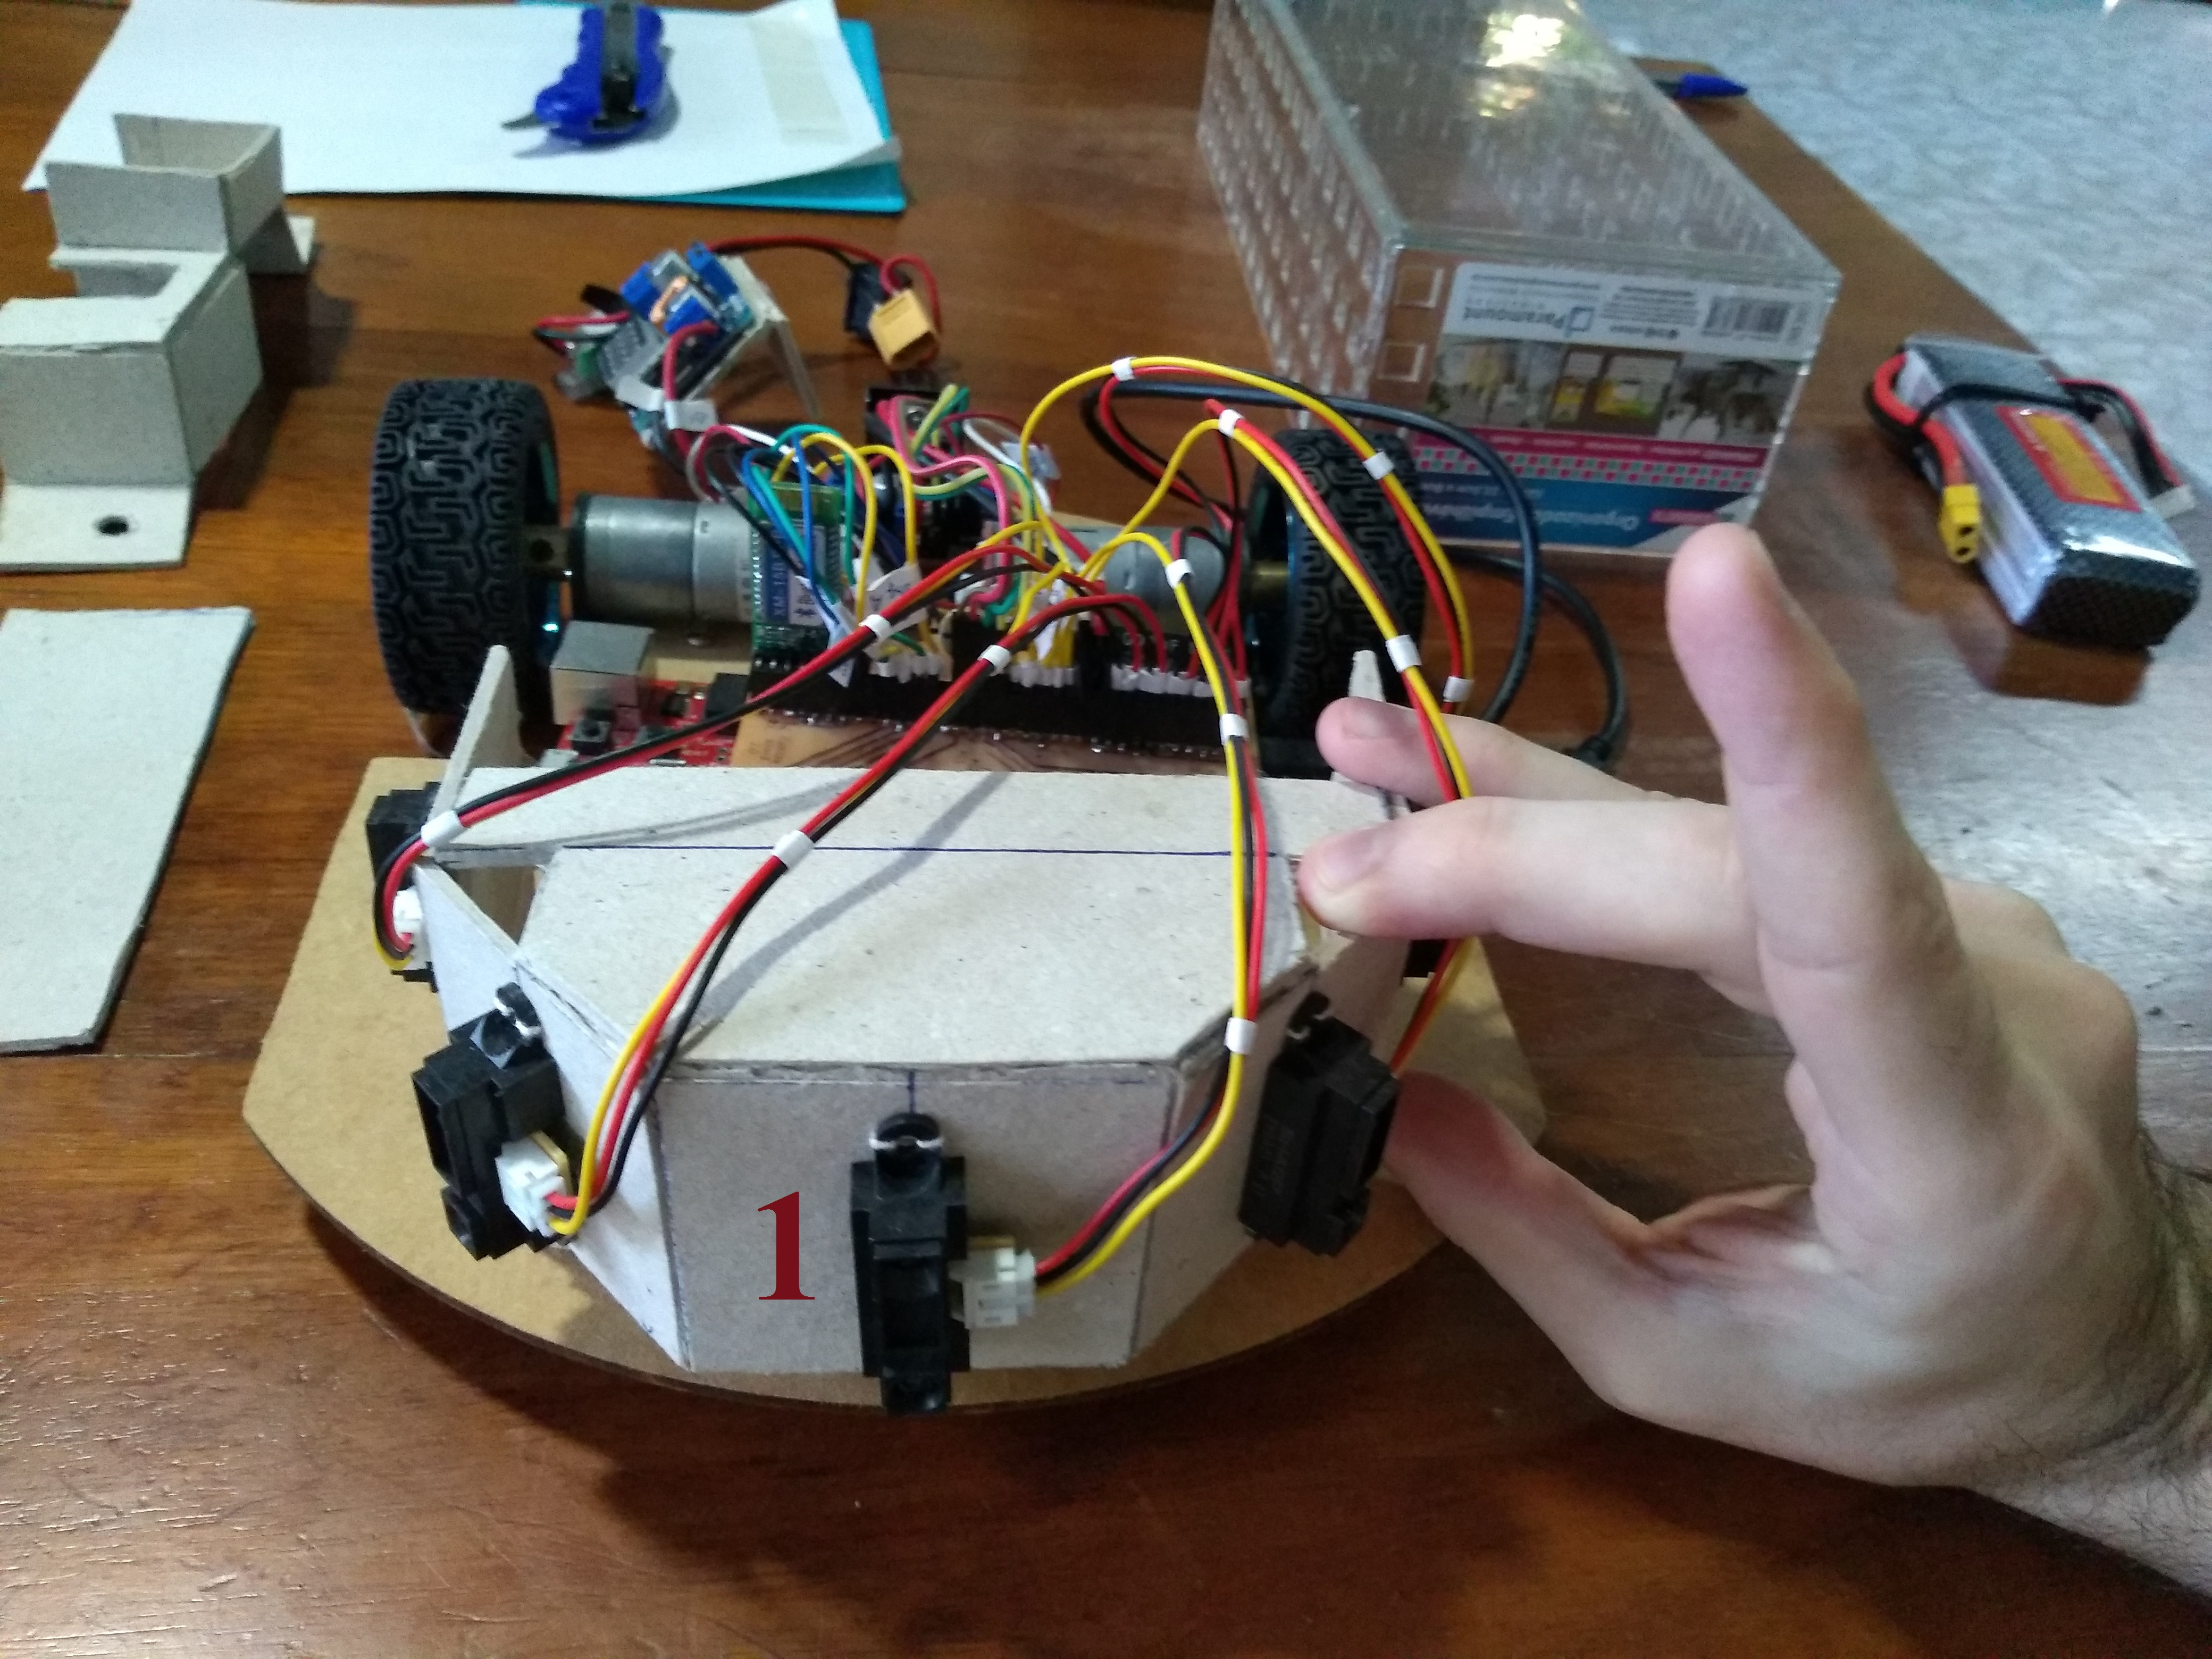
\includegraphics[trim= 0cm 0cm 0cm 0cm,clip,
scale=0.055]{Figuras/RoboMontagem1}
		\subcaption{Posicionamento dos sensores IR}
	  	%\label{fig:test1}
	\end{subfigure}
	~
	\begin{subfigure}[b]{0.49\textwidth}%
		\centering
		% fbox{}
		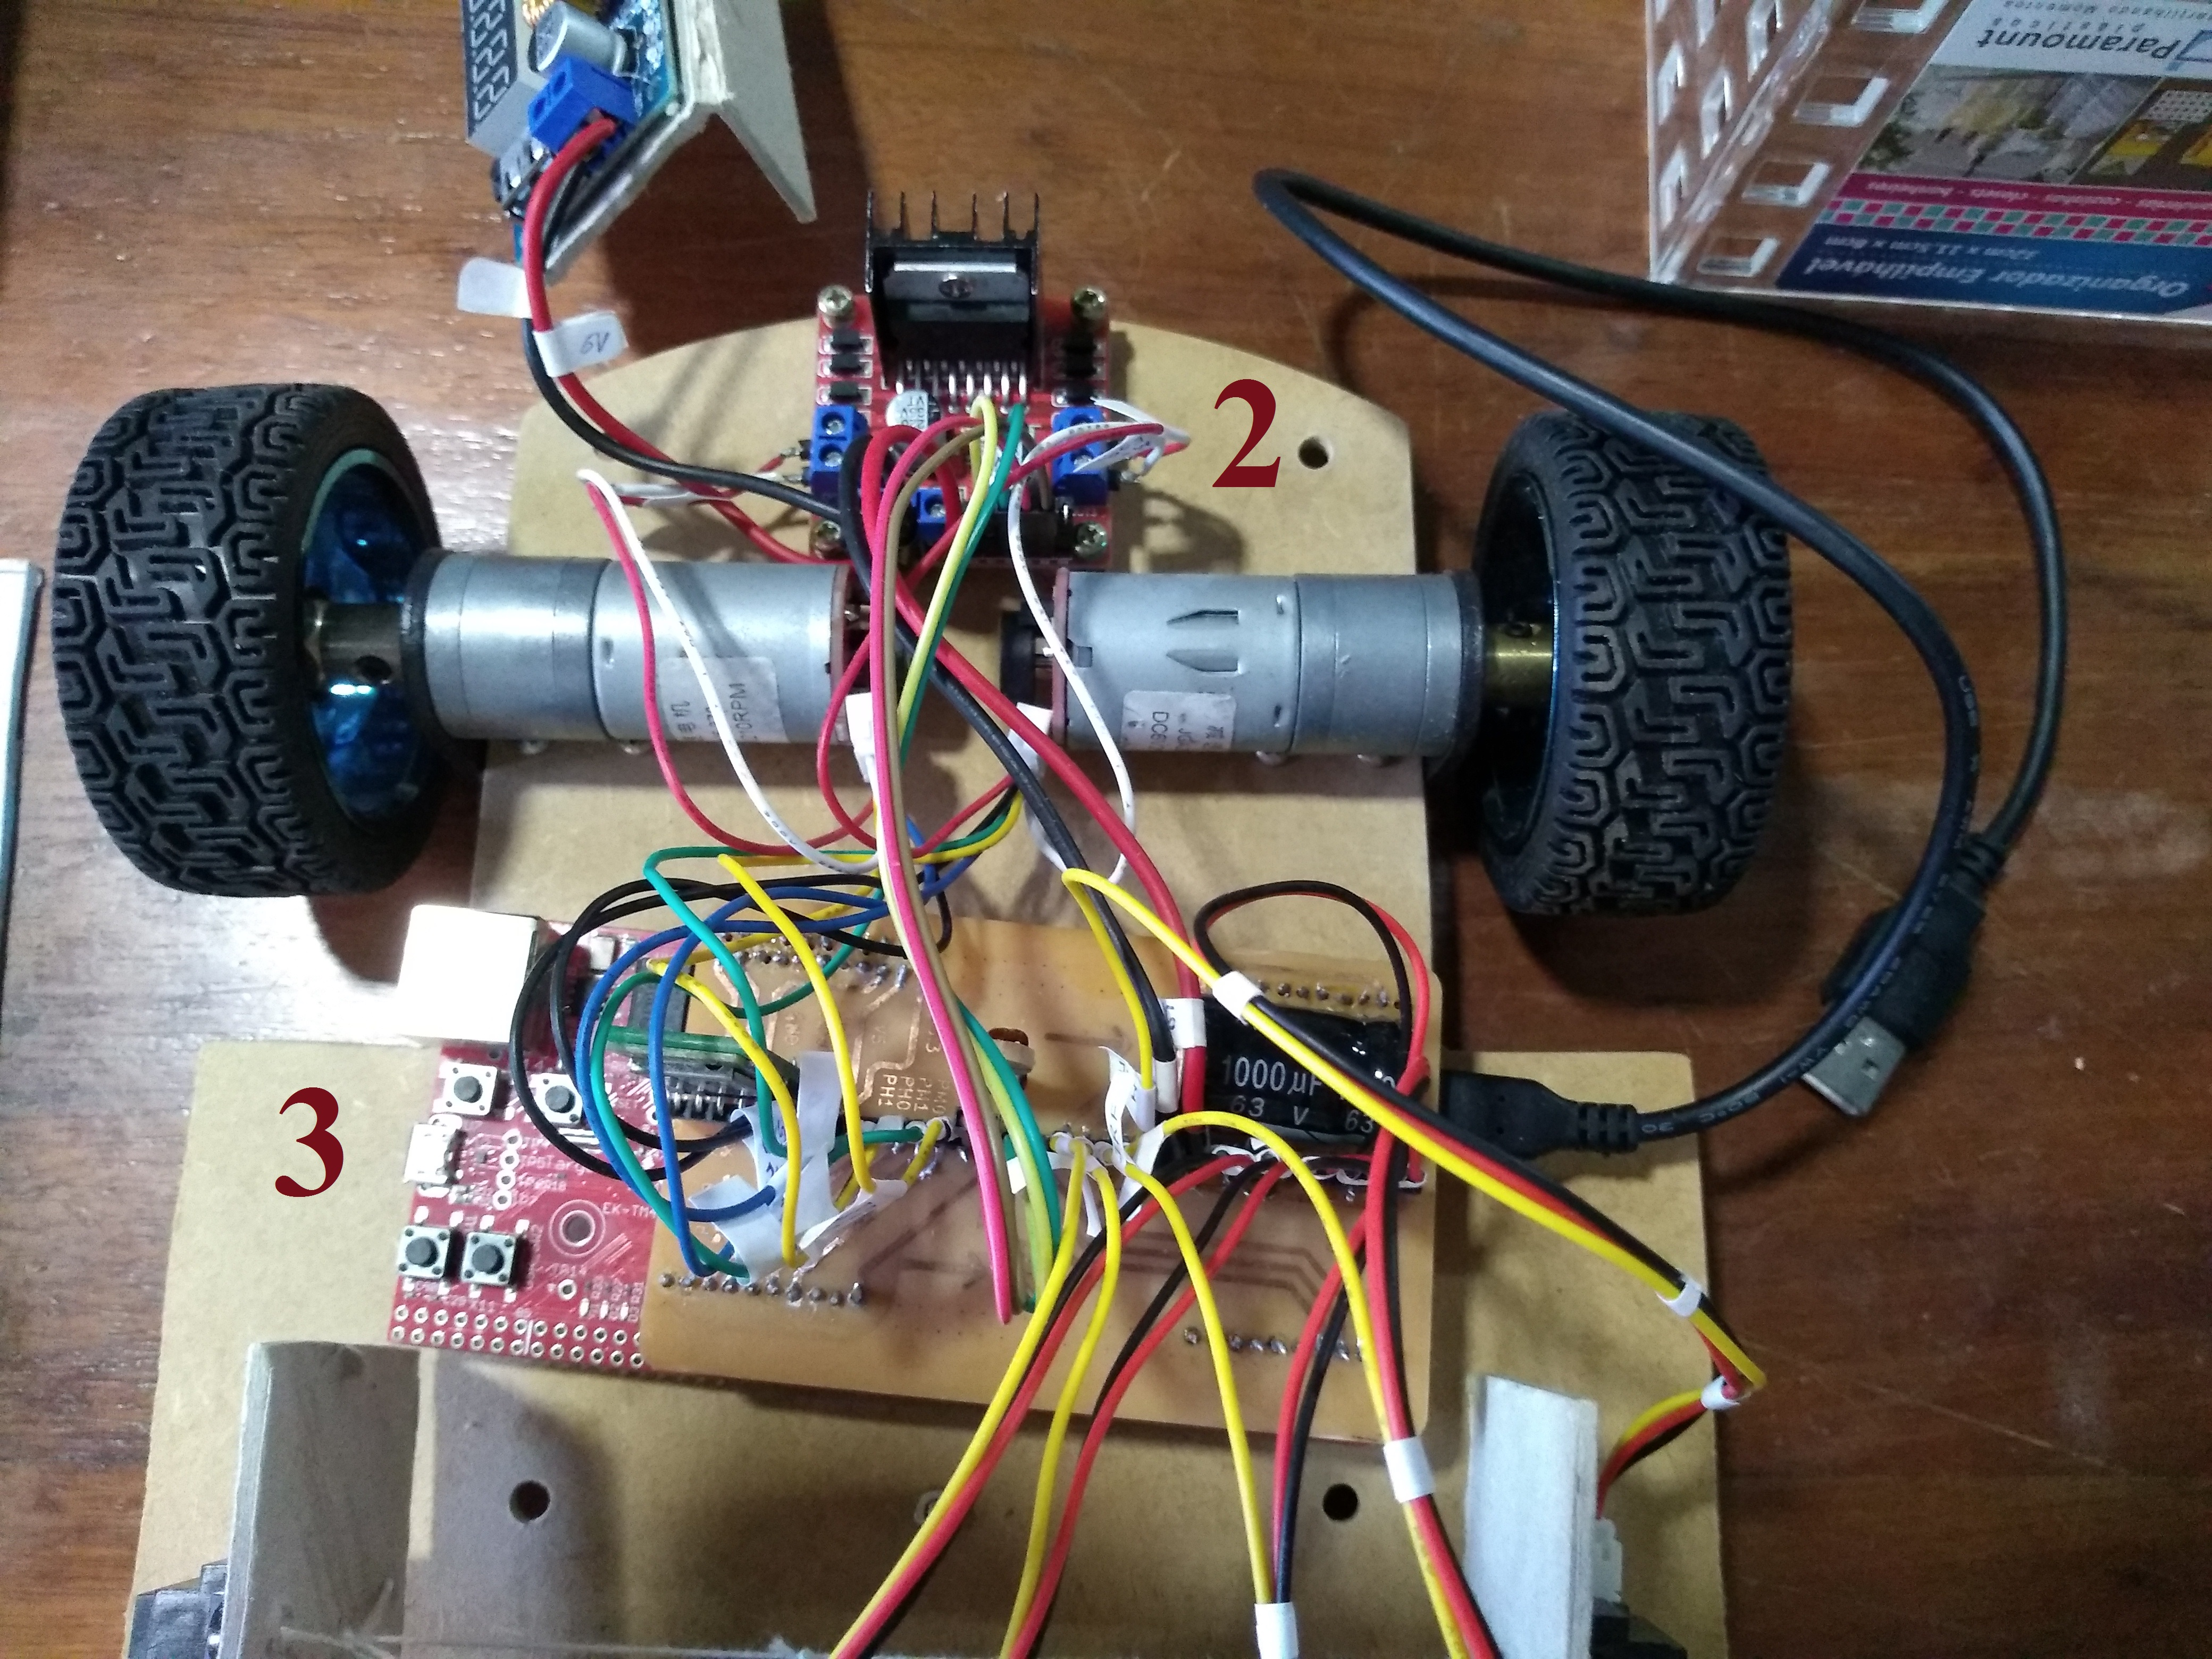
\includegraphics[trim={0cm 0cm 0cm 0cm},clip,
scale=0.055]{Figuras/RoboMontagem2}
		\subcaption{Disposição dos motores e microcontrolador}
	  	%\label{fig:test2}
	\end{subfigure}
	~
	\begin{subfigure}[b]{0.49\textwidth}%
		\centering
		% fbox{}
		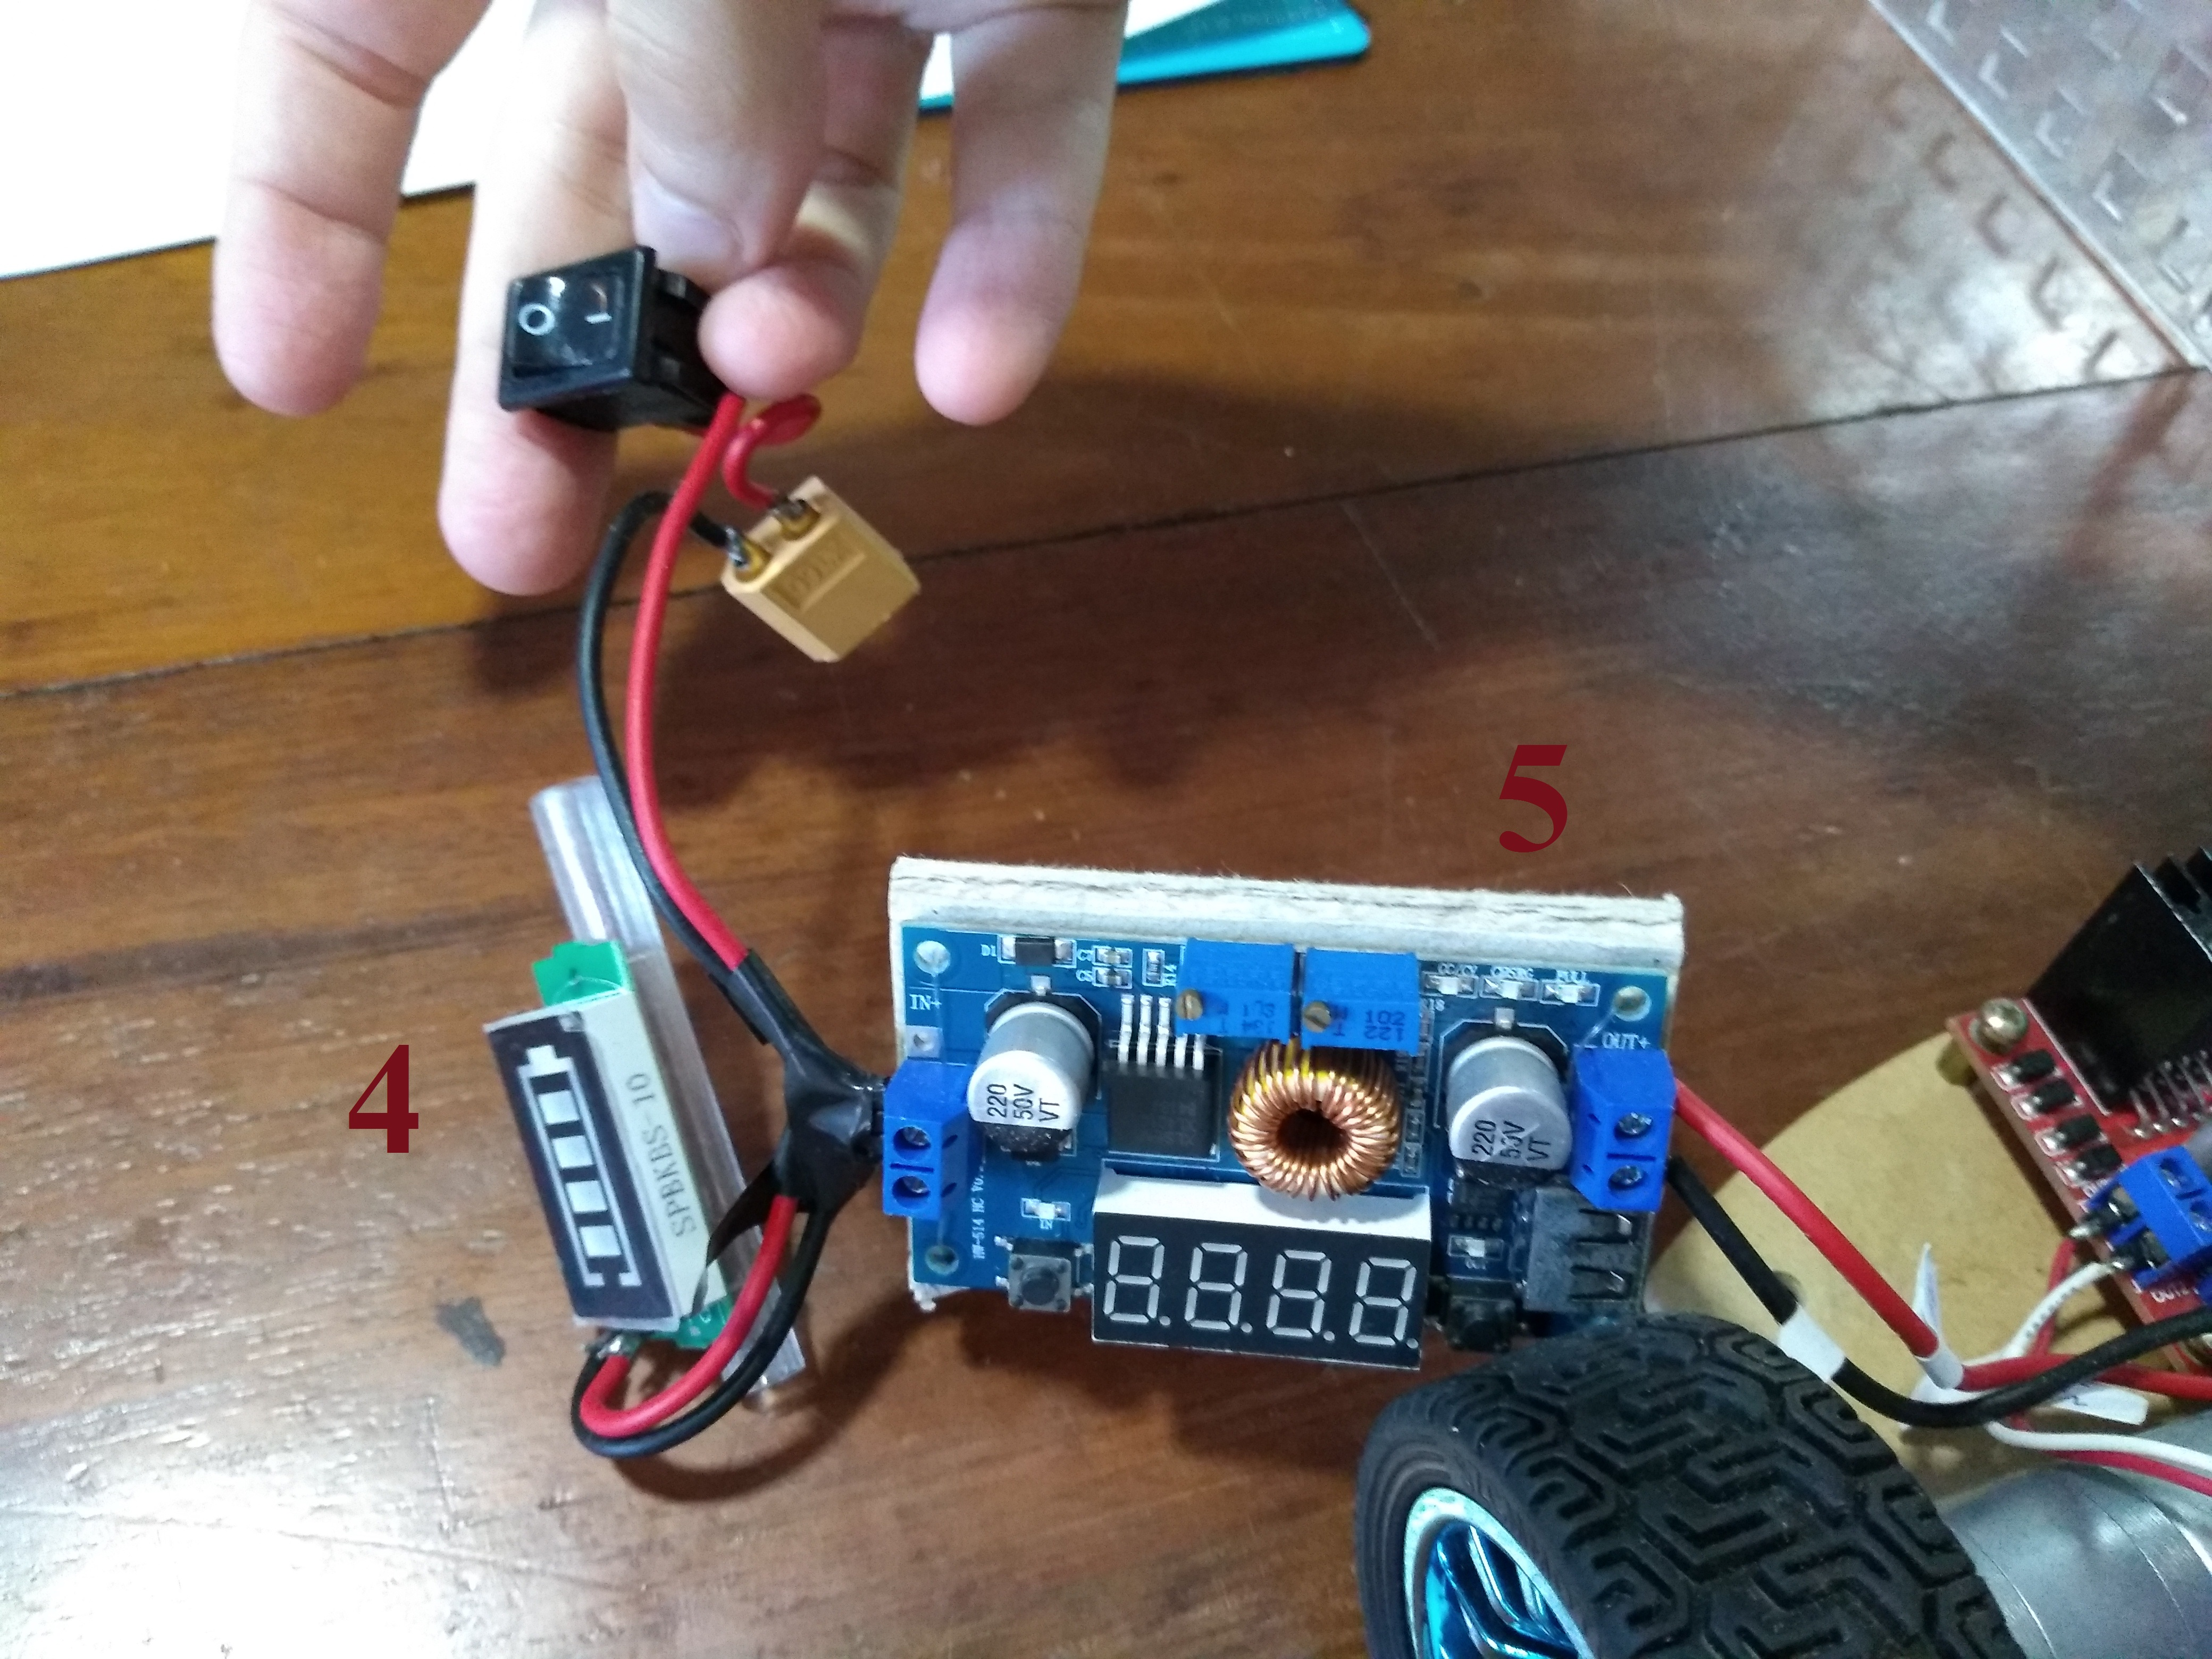
\includegraphics[trim= 0cm 0cm 0cm 0cm,clip,
scale=0.055]{Figuras/RoboMontagem3}
		\subcaption{Regulador de Tensão}
	  	%\label{fig:test1}
	\end{subfigure}
	~
	\begin{subfigure}[b]{0.49\textwidth}%
		\centering
		% fbox{}
		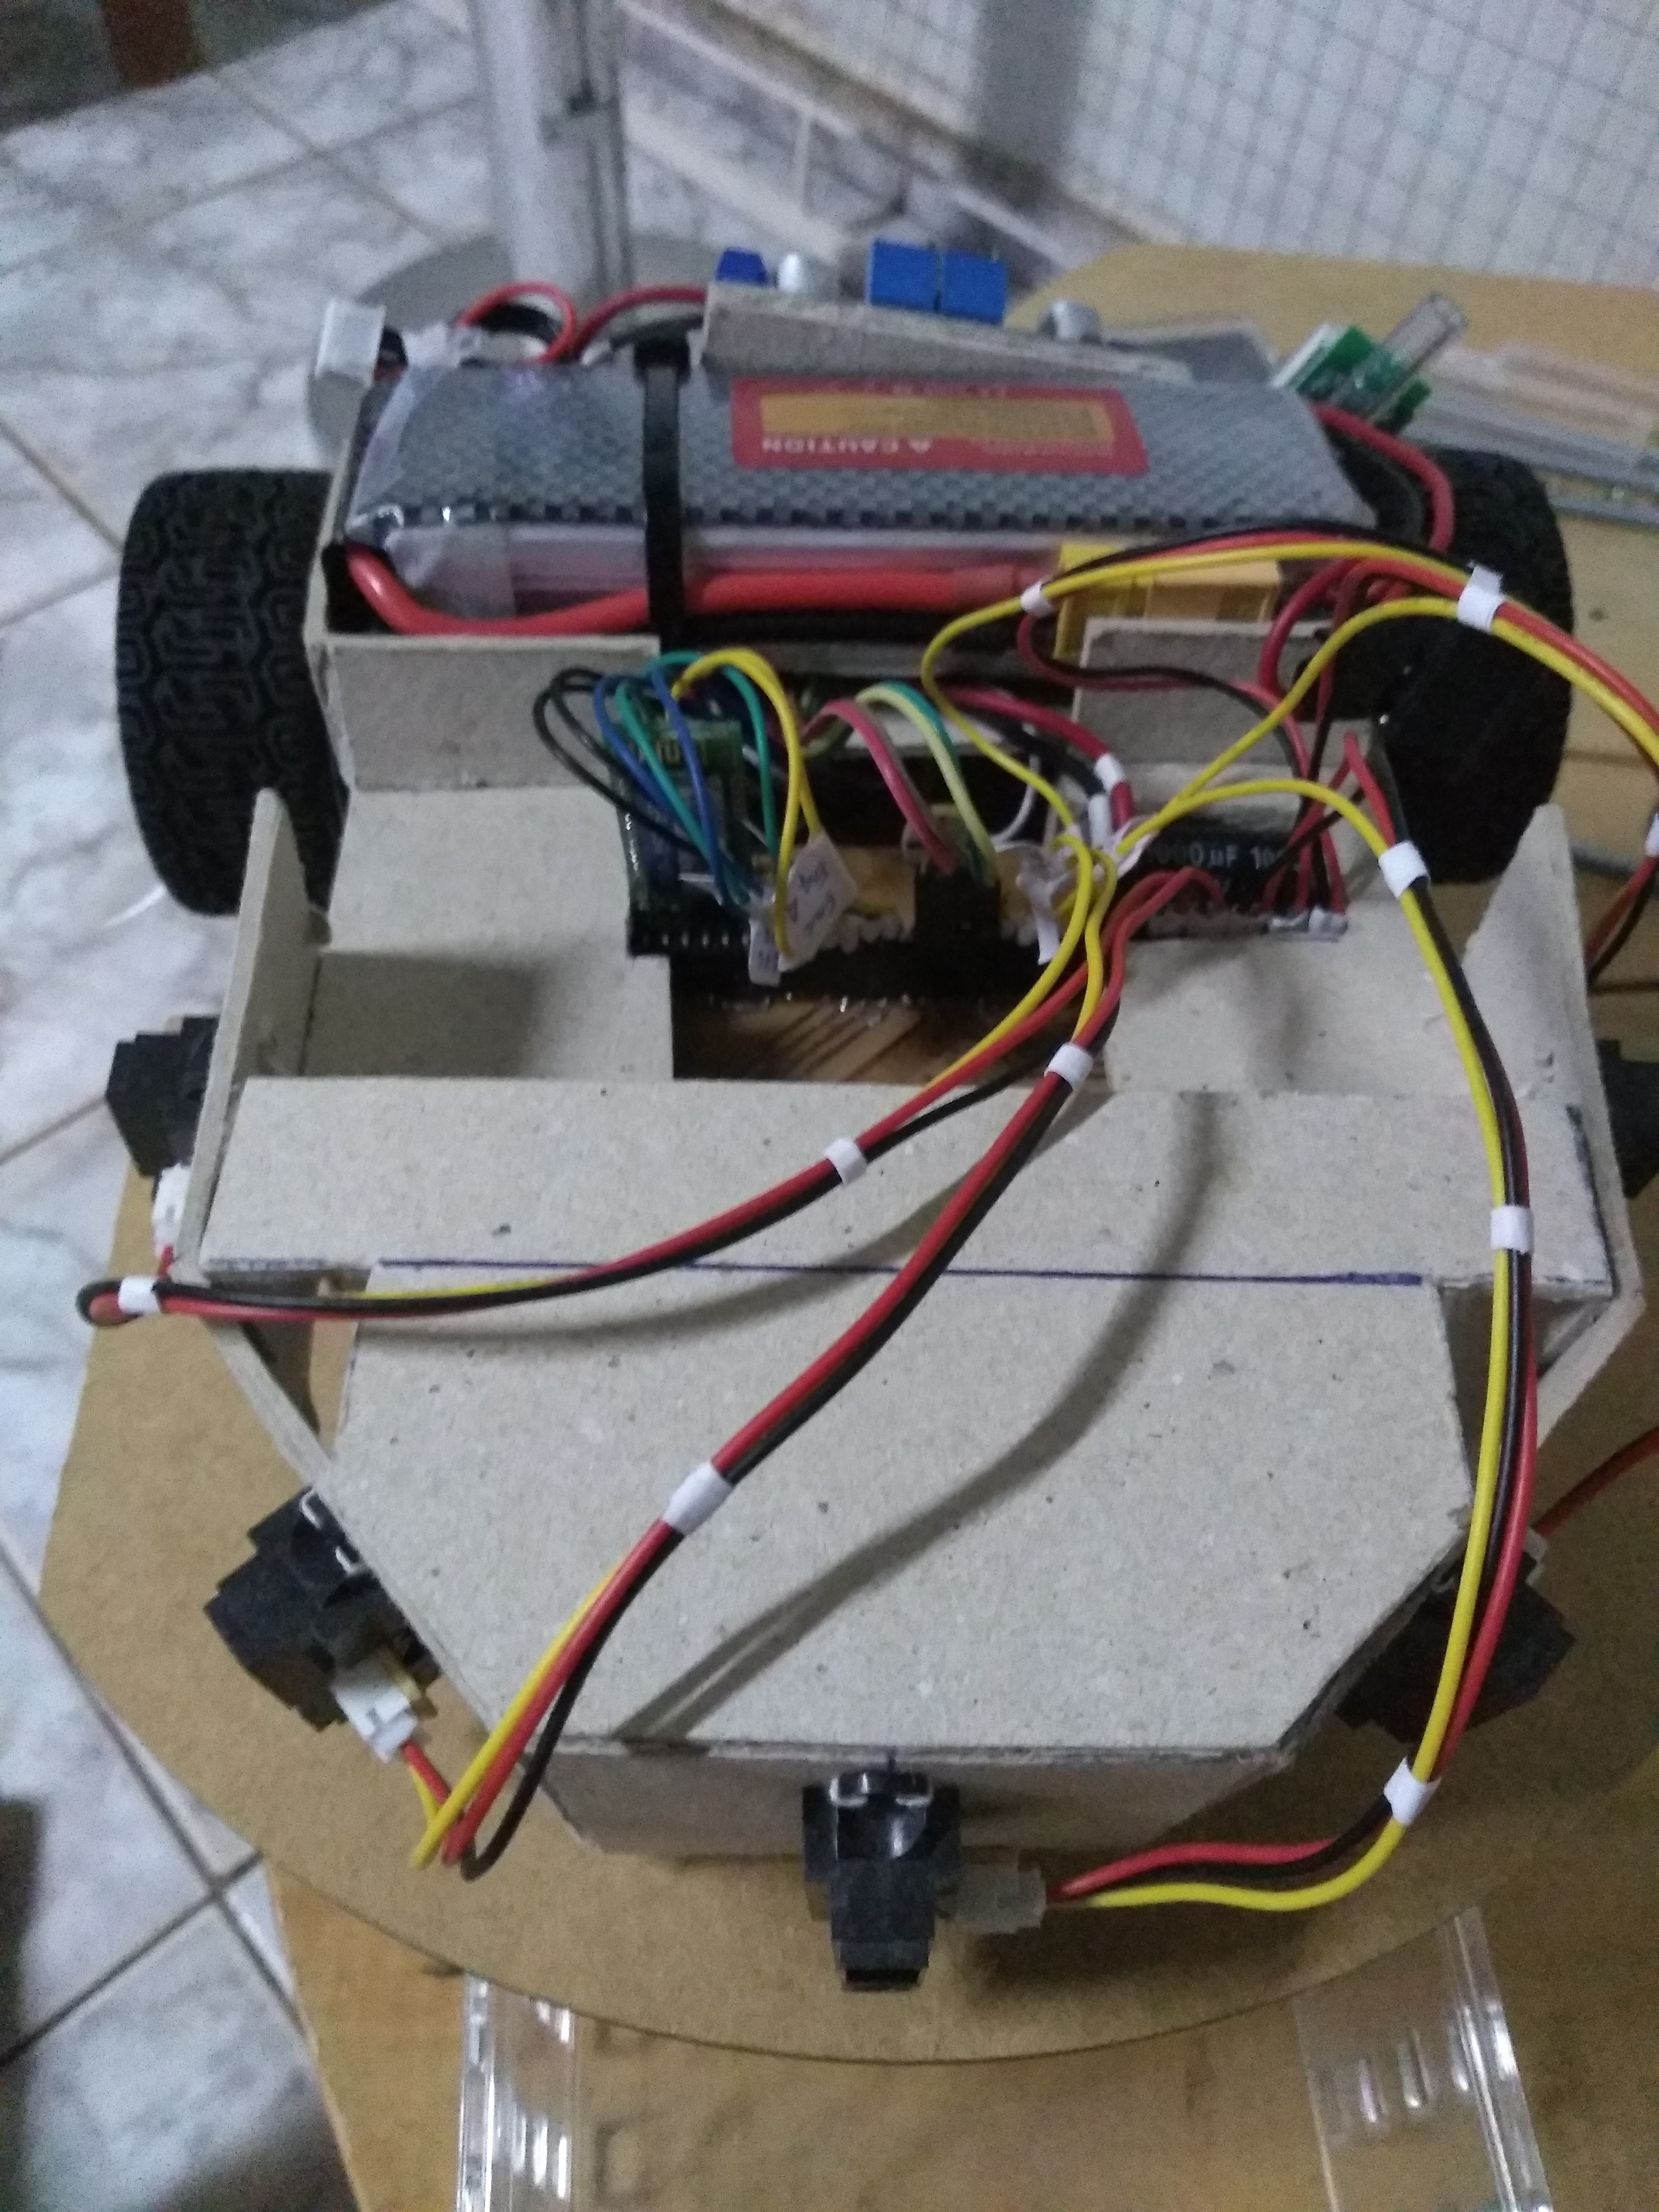
\includegraphics[trim={0cm 0cm 0cm 0cm},clip,
scale=0.055]{Figuras/RoboMontagem4}
		\subcaption{Posicionamento dos componentes}
	  	%\label{fig:test2}
	\end{subfigure}
	
	\textbf{Fonte: autoria própria}
\end{figure}
	
	O número 1 na Figura \ref{fig:RoboReal}.a indica o sensor infravermelho. Os números 2 e 3
	na Figura \ref{fig:RoboReal}.b indicam o driver e o microcontrolador, respectivamente.
	Os números 4 e 5 na Figura \ref{fig:RoboReal}.c indicam, respectivamente, o exibidor
	de nível energia para bateria de lítio (que não é necessário para o funcionamento) 
	e o regulador de tensão regulável. 
	
	A Figura \ref{fig:RoboReal2}.a mostra o posicionamento dos periféricos e parafusos 
	roscados. A Figura \ref{fig:RoboReal2}.b retrata a montagem concluída.
	
	\begin{figure}[!ht]
\centering
\caption{Robô após montagem}
\label{fig:RoboReal2}
	\begin{subfigure}[b]{0.49\textwidth}%
		\centering
		% fbox{}
		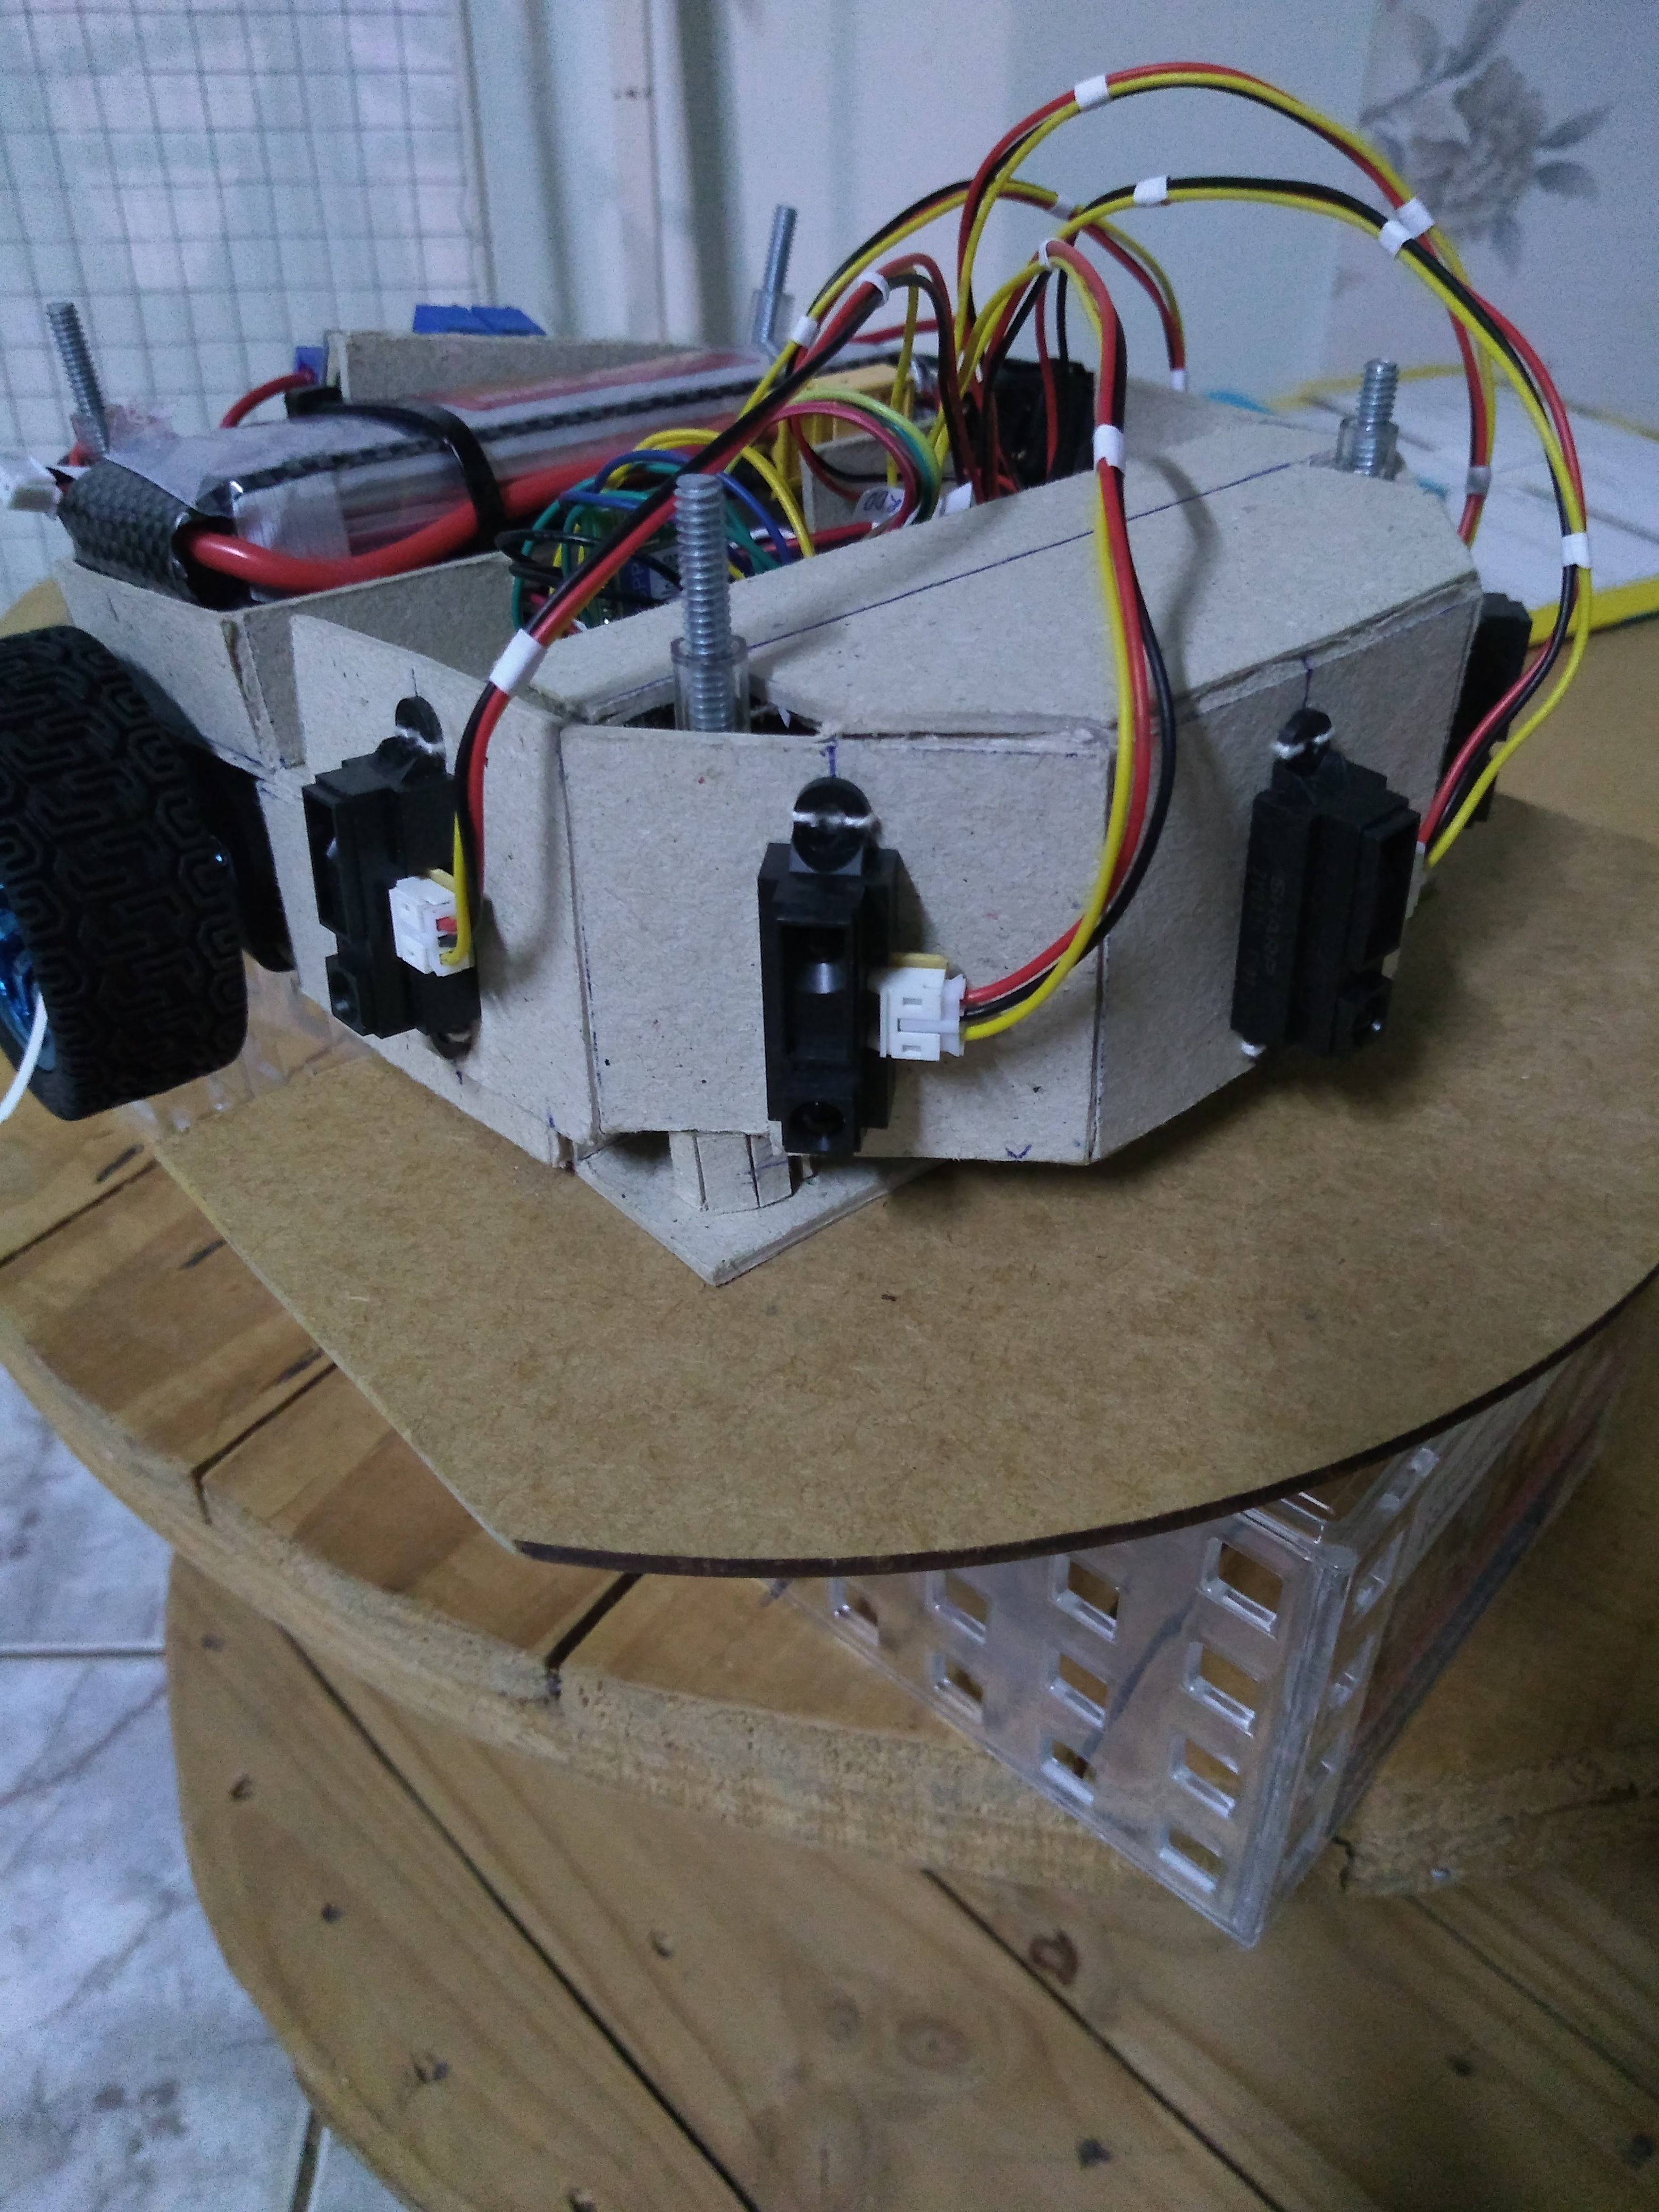
\includegraphics[trim={0cm 35cm 0cm 0cm}, clip, 
		scale=0.055]{Figuras/RoboMontagem5}
		\subcaption{Posição dos parafusos de rosca}
	  	%\label{fig:test1}
	\end{subfigure}
	~
	\begin{subfigure}[b]{0.49\textwidth}%
		\centering
		% fbox{}
		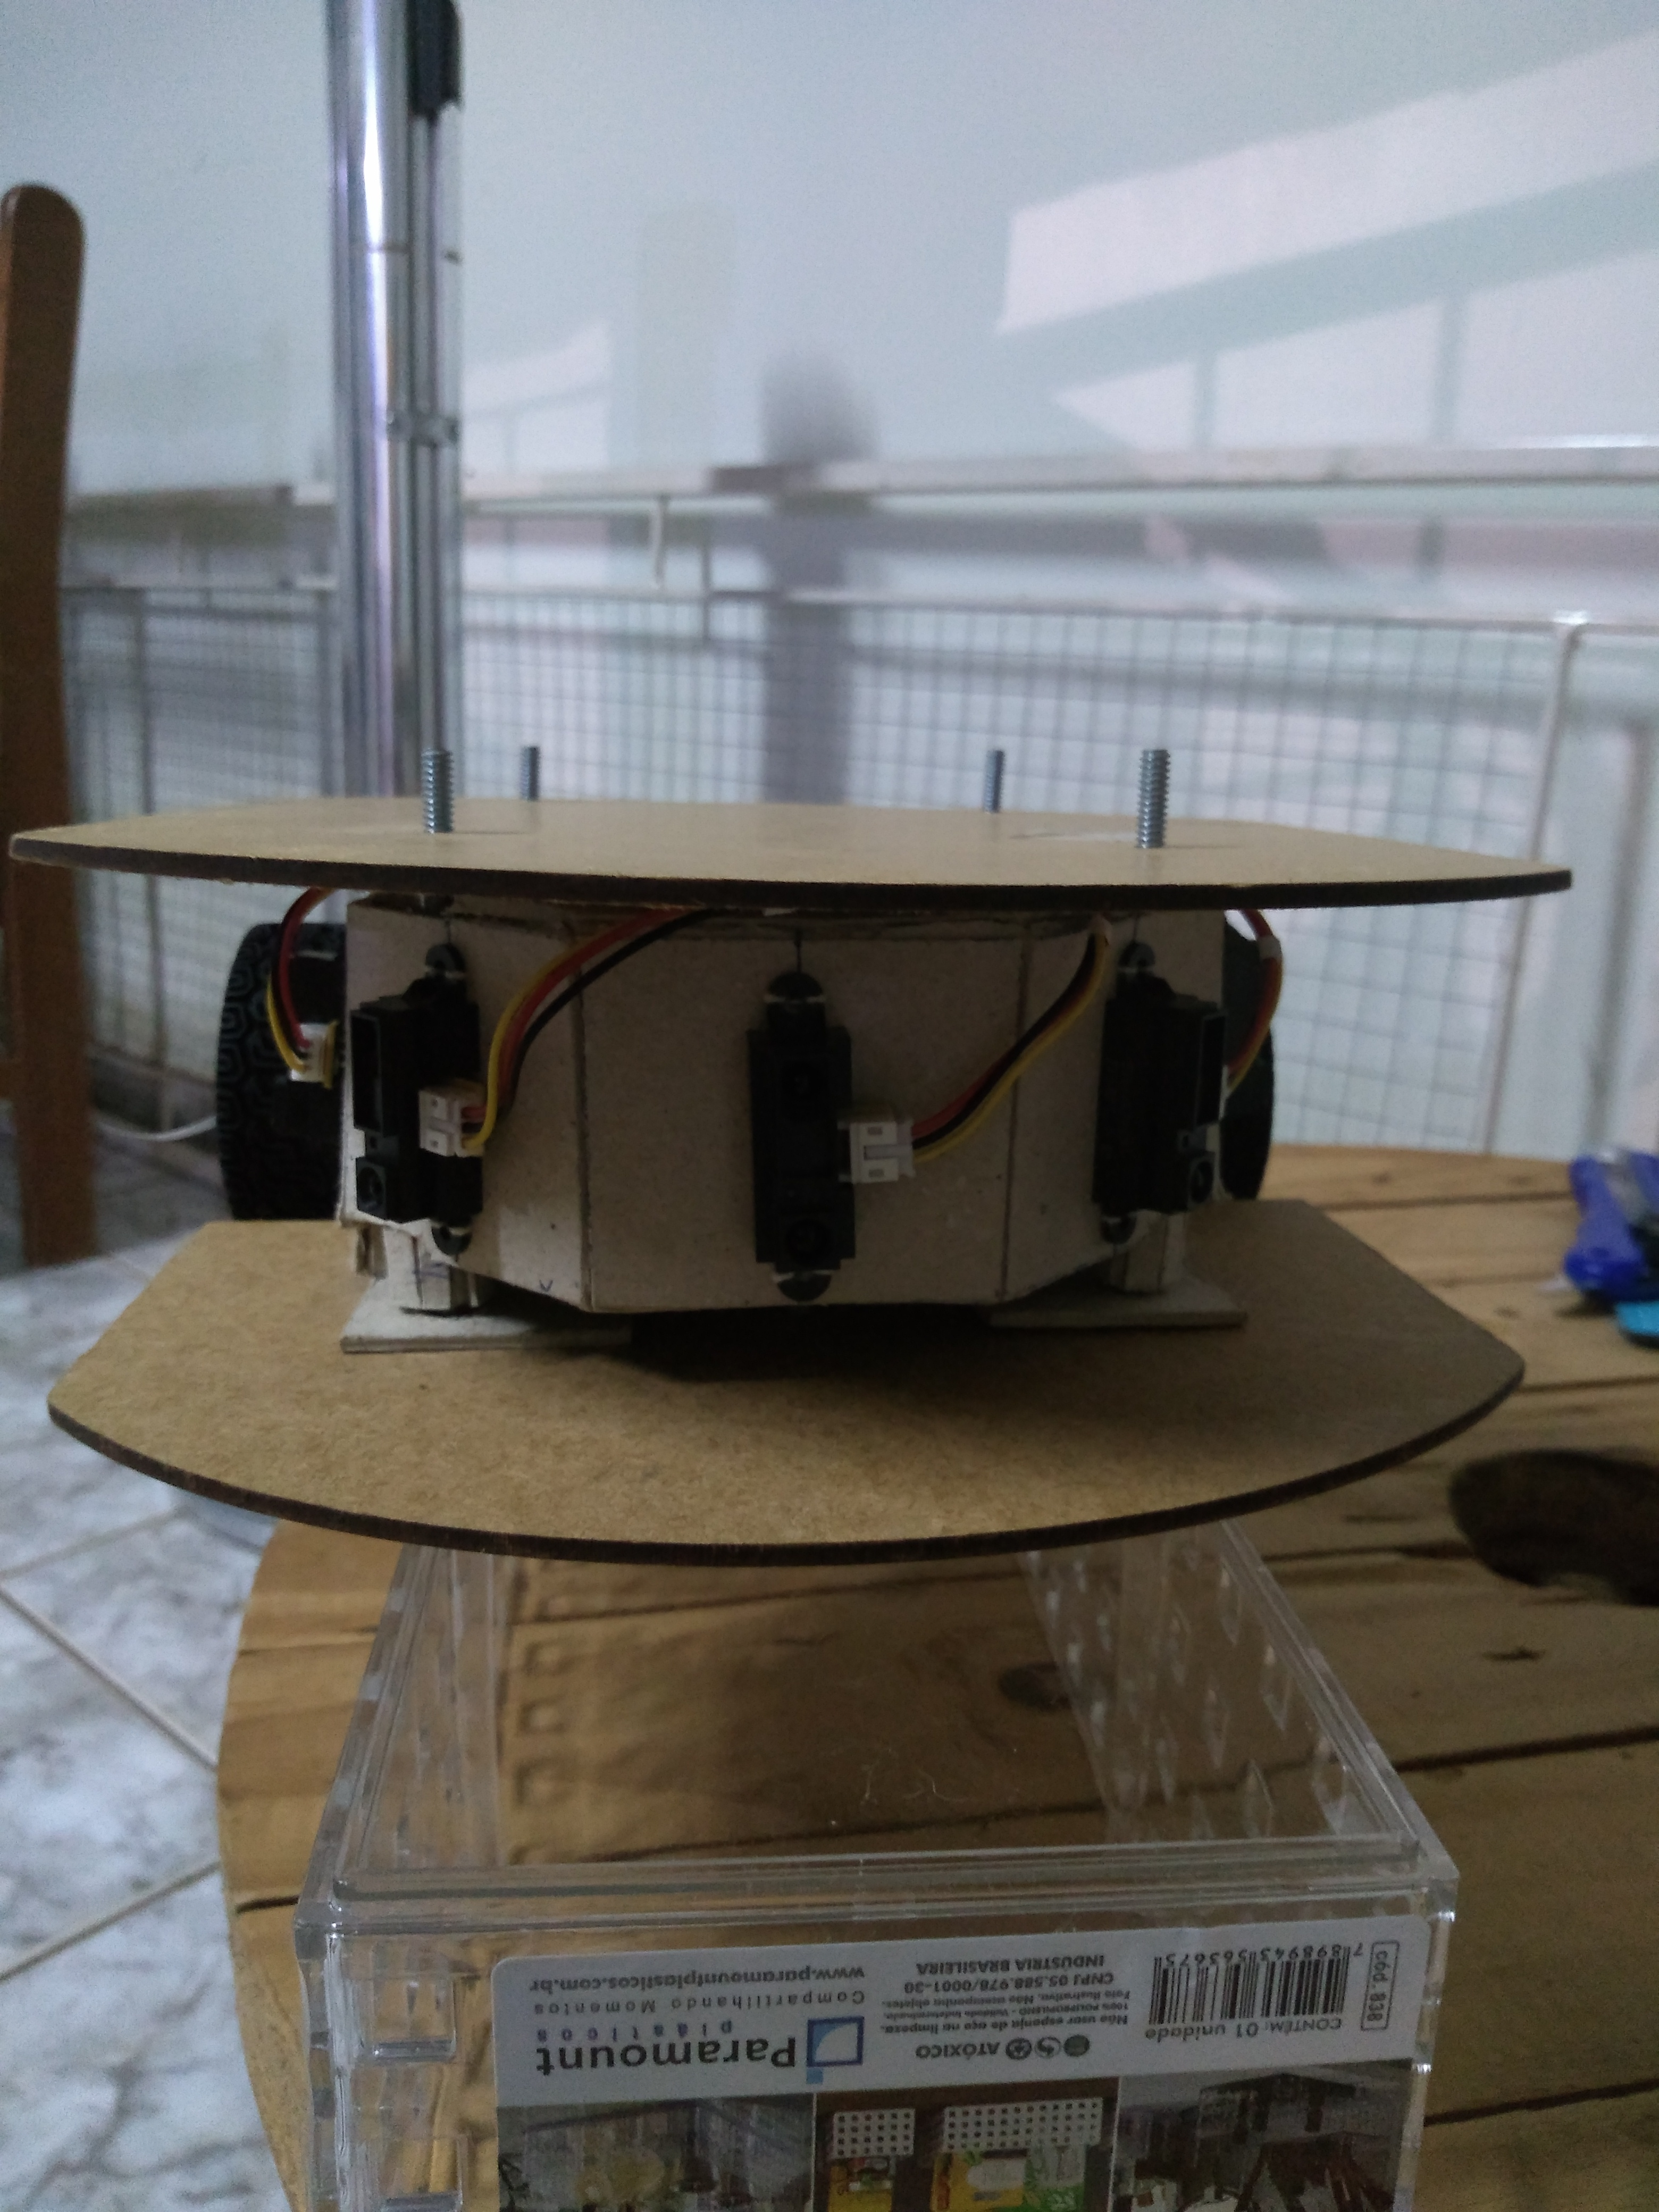
\includegraphics[trim={0cm 12.5cm 0cm 22.5cm}, clip, 
		scale=0.055]{Figuras/RoboMontagem6}
		\subcaption{Robô montado}
	  	%\label{fig:test2}
	\end{subfigure}
	\textbf{Fonte: autoria própria}
\end{figure}
	
\subsubsection{Curvas dos motores}

	A partir de um requisito de velocidade angular, é necessário definir a quantidade de 
	acionamento que será utilizada no motor (porcentagem de PWM).
	
	Para isso, foi feito um levantamento da curva dos motores. Ao alterar a porcentagem do
	acionamento PWM com incrementos de 1\%, a saída do sensor de efeito \textit{hall} é 
	utilizada para calcular a velocidade em rotações por segundo. 
	
	A Figura \ref{fig:acionamento1} mostra essa curva para o caso de ausência de carga, ou
	seja, o teste foi realizado sem que o pneu tocasse o chão. 
	
	\begin{figure}[!ht]
\centering
\caption{Curva do motor sem carga}
\label{fig:acionamento1}
		\centering
		% fbox{}
		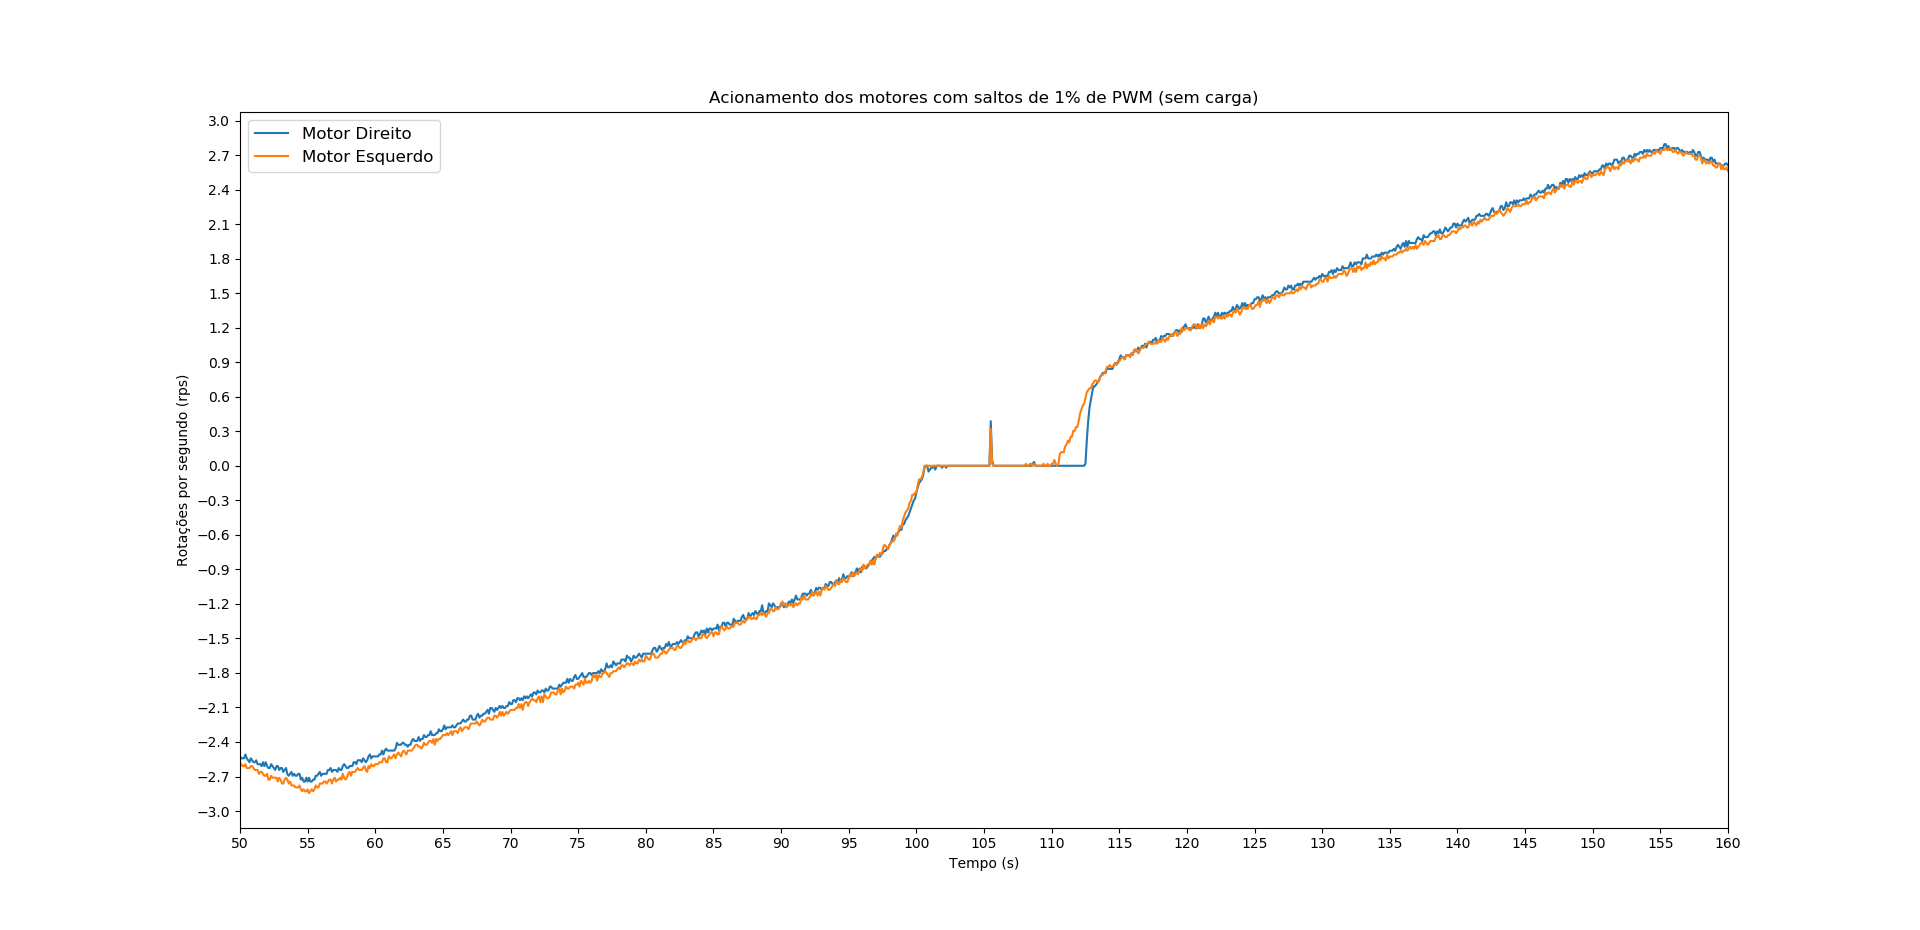
\includegraphics[trim={5cm 1cm 5cm 2cm},clip,
scale=0.38]{Figuras/Acionamento_Sem_Carga_rps}
	
	\textbf{Fonte: autoria própria}
\end{figure}
	
	A Figura \ref{fig:acionamento2} mostra a curva para o caso de presença de carga. Neste
	caso, o teste foi feito com o robô no chão, em uma quadra de esportes que, por não ter 
	o chão tão liso, levou a um gráfico bastante ruidoso. Os três pontos fora da curva 
	ocorreram devido a pequenos chutes dados no robô a fim de evitar uma colisão com parede.
	
	\begin{figure}[!ht]
\centering
\caption{Curva do motor com carga}
\label{fig:acionamento2}
		\centering
		% fbox{}
		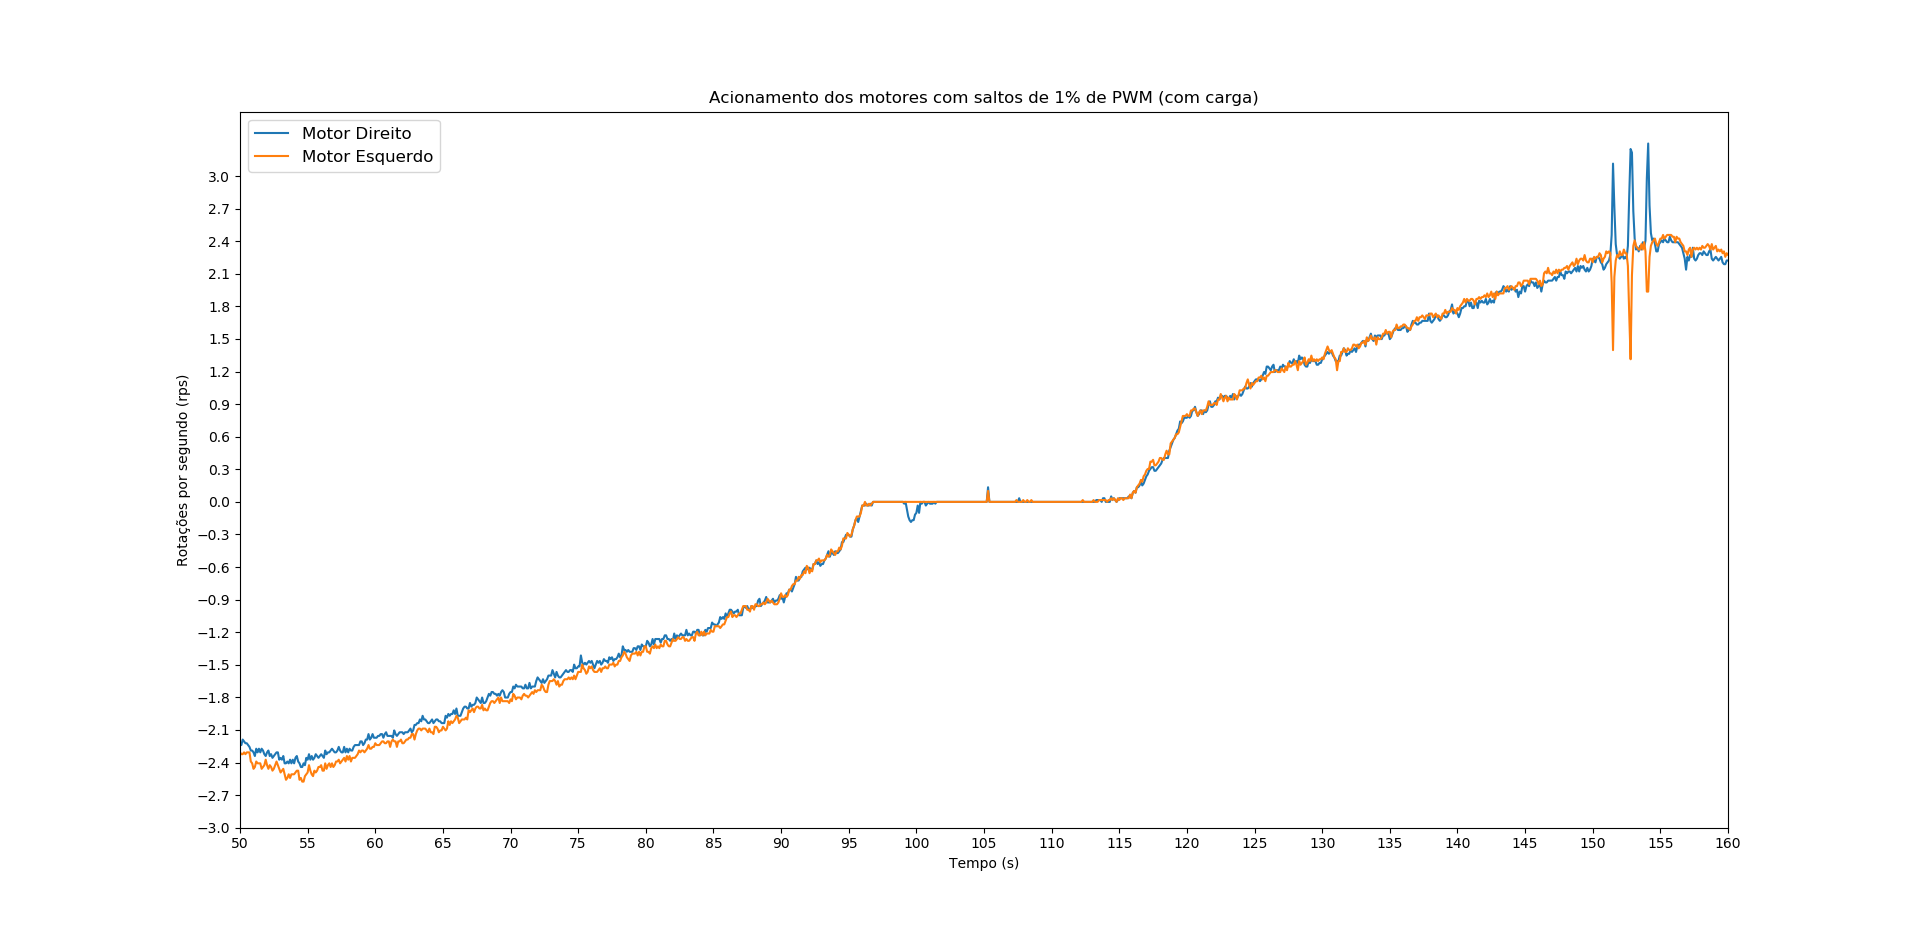
\includegraphics[trim={4.4cm 1cm 4.5cm 2cm},clip,
scale=0.38]{Figuras/Acionamento_Com_Carga_rps}
	
	\textbf{Fonte: autoria própria}
\end{figure}
	
	A partir do teste sem carga do motor direito, foi feita uma regressão linear utilizando 
	a parte da curva cujo regime é linear. A Figura \ref{fig:acionamento3} mostra o resultado 
	dessa regressão, bem como as constantes obtidas.
	
	\begin{figure}[!ht]
\centering
\caption{Regressão Linear para a curva do motor}
\label{fig:acionamento3}
		\centering
		% fbox{}
		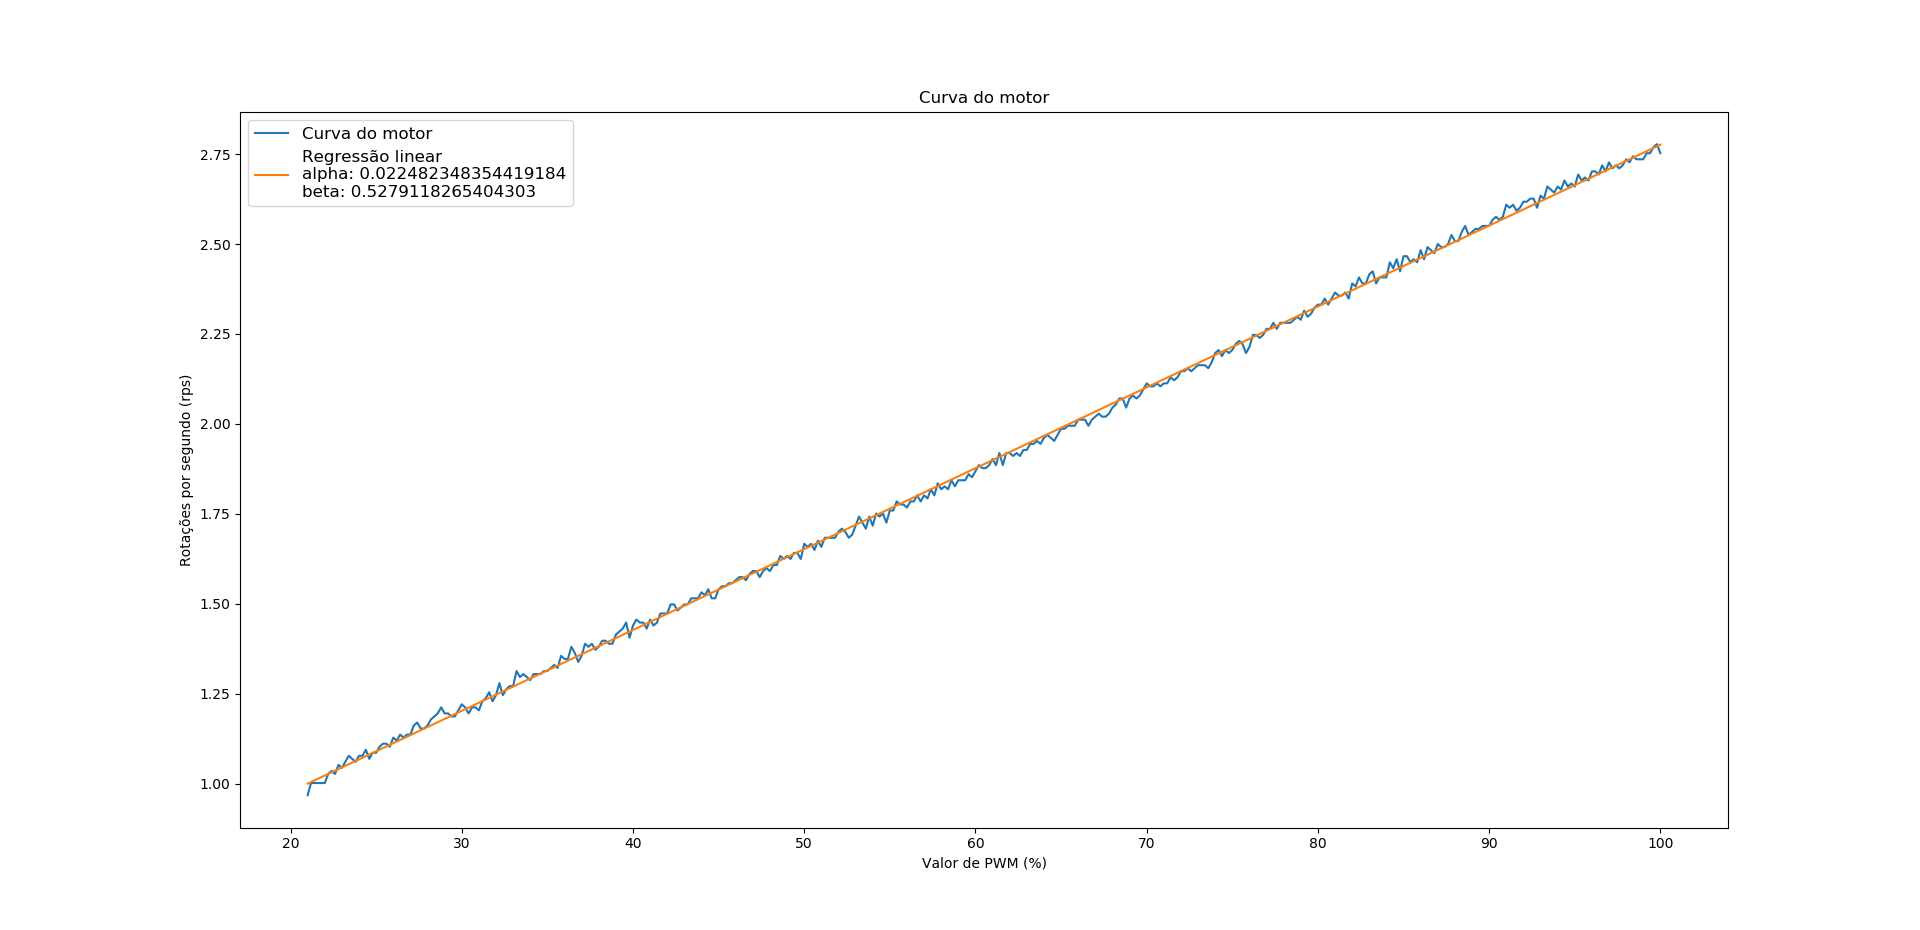
\includegraphics[trim={5cm 1cm 5cm 2cm},clip,
scale=0.38]{Figuras/Curva_Do_Motor_rps}
	
	\textbf{Fonte: autoria própria}
\end{figure}
	
\section{Metodologia}

Neste trabalho o protótipo será desenvolvido tendo como base o robô móvel de
acionamento diferencial Quickbot \cite{QuickBot}. Porém, esse robô se encontra
com alguns componentes de hardware obsoletos. Componentes mais atuais serão
utilizados.

O simulador Simiam será estudado de modo a permitir a inserção de novas
funcionalidades, como o módulo \textit{fuzzy}, pois este simulador foi
implementado visando a utilização de uma arquitetura de controle híbrida (SED em conjunto
com SDVC). 

Em seguida, deve-se projetar os comportamentos do robô que solucionem o problema
proposto de duas maneiras separadas: utilizando o sistema híbrido, a fim de estudar a
estratégia de arbitragem de comportamentos, e por sistema \textit{fuzzy}, a fim de compreender 
a estratégia de fusão de comportamentos. 

Utilizar o simulador Simiam, desenvolvido pela Universidade Georgia
Tech, para validar o algoritmo de controle.

Deve-se executar a montagem física, implementar o sistema embarcado e elaborar os testes em
protótipo, utilizando obstáculos em posições distintas a fim de verificar a robustez dos 
algoritmos implementados. 
\chapter{Desenvolvimento}
\vspace{-2.5 cm}

% Este Capítulo apresenta o que foi desenvolvido até o momento.
Este Capítulo apresenta o que foi desenvolvido como resultado deste trabalho,
visando alcançar os objetivos propostos.

\section{O simulador Simiam e alterações necessárias}

O Simulador Simiam foi implementado pela Universidade Georgia Tech, 
inicialmente oferecendo apenas suporte ao robô Khepera 3. Posteriormente, 
para atender necessidades do curso \textit{Control of Mobile Robots}, hospedado 
na plataforma ``Coursera.org'', o robô de baixo custo QuickBot foi adicionado. 
Os robôs Khepera e QuickBot reais podem ser vistos na Figura \ref{fig:RobosK3QB}. 
Suas contrapartes simuladas estão retratadas na Figura \ref{fig:RobosEmSimulador}.

O curso mencionado foi removido da plataforma no dia 17 de Agosto de 2020 e apenas
os alunos concluíntes possuem acesso. De qualquer forma, o simulador ainda pode ser
obtido gratuitamente.

\begin{figure}[ht]
\centering
\caption{Robôs Khepera 3 e QuickBot}
\label{fig:RobosK3QB}
	\begin{subfigure}[b]{0.49\textwidth}%
		\centering
		% fbox{}
		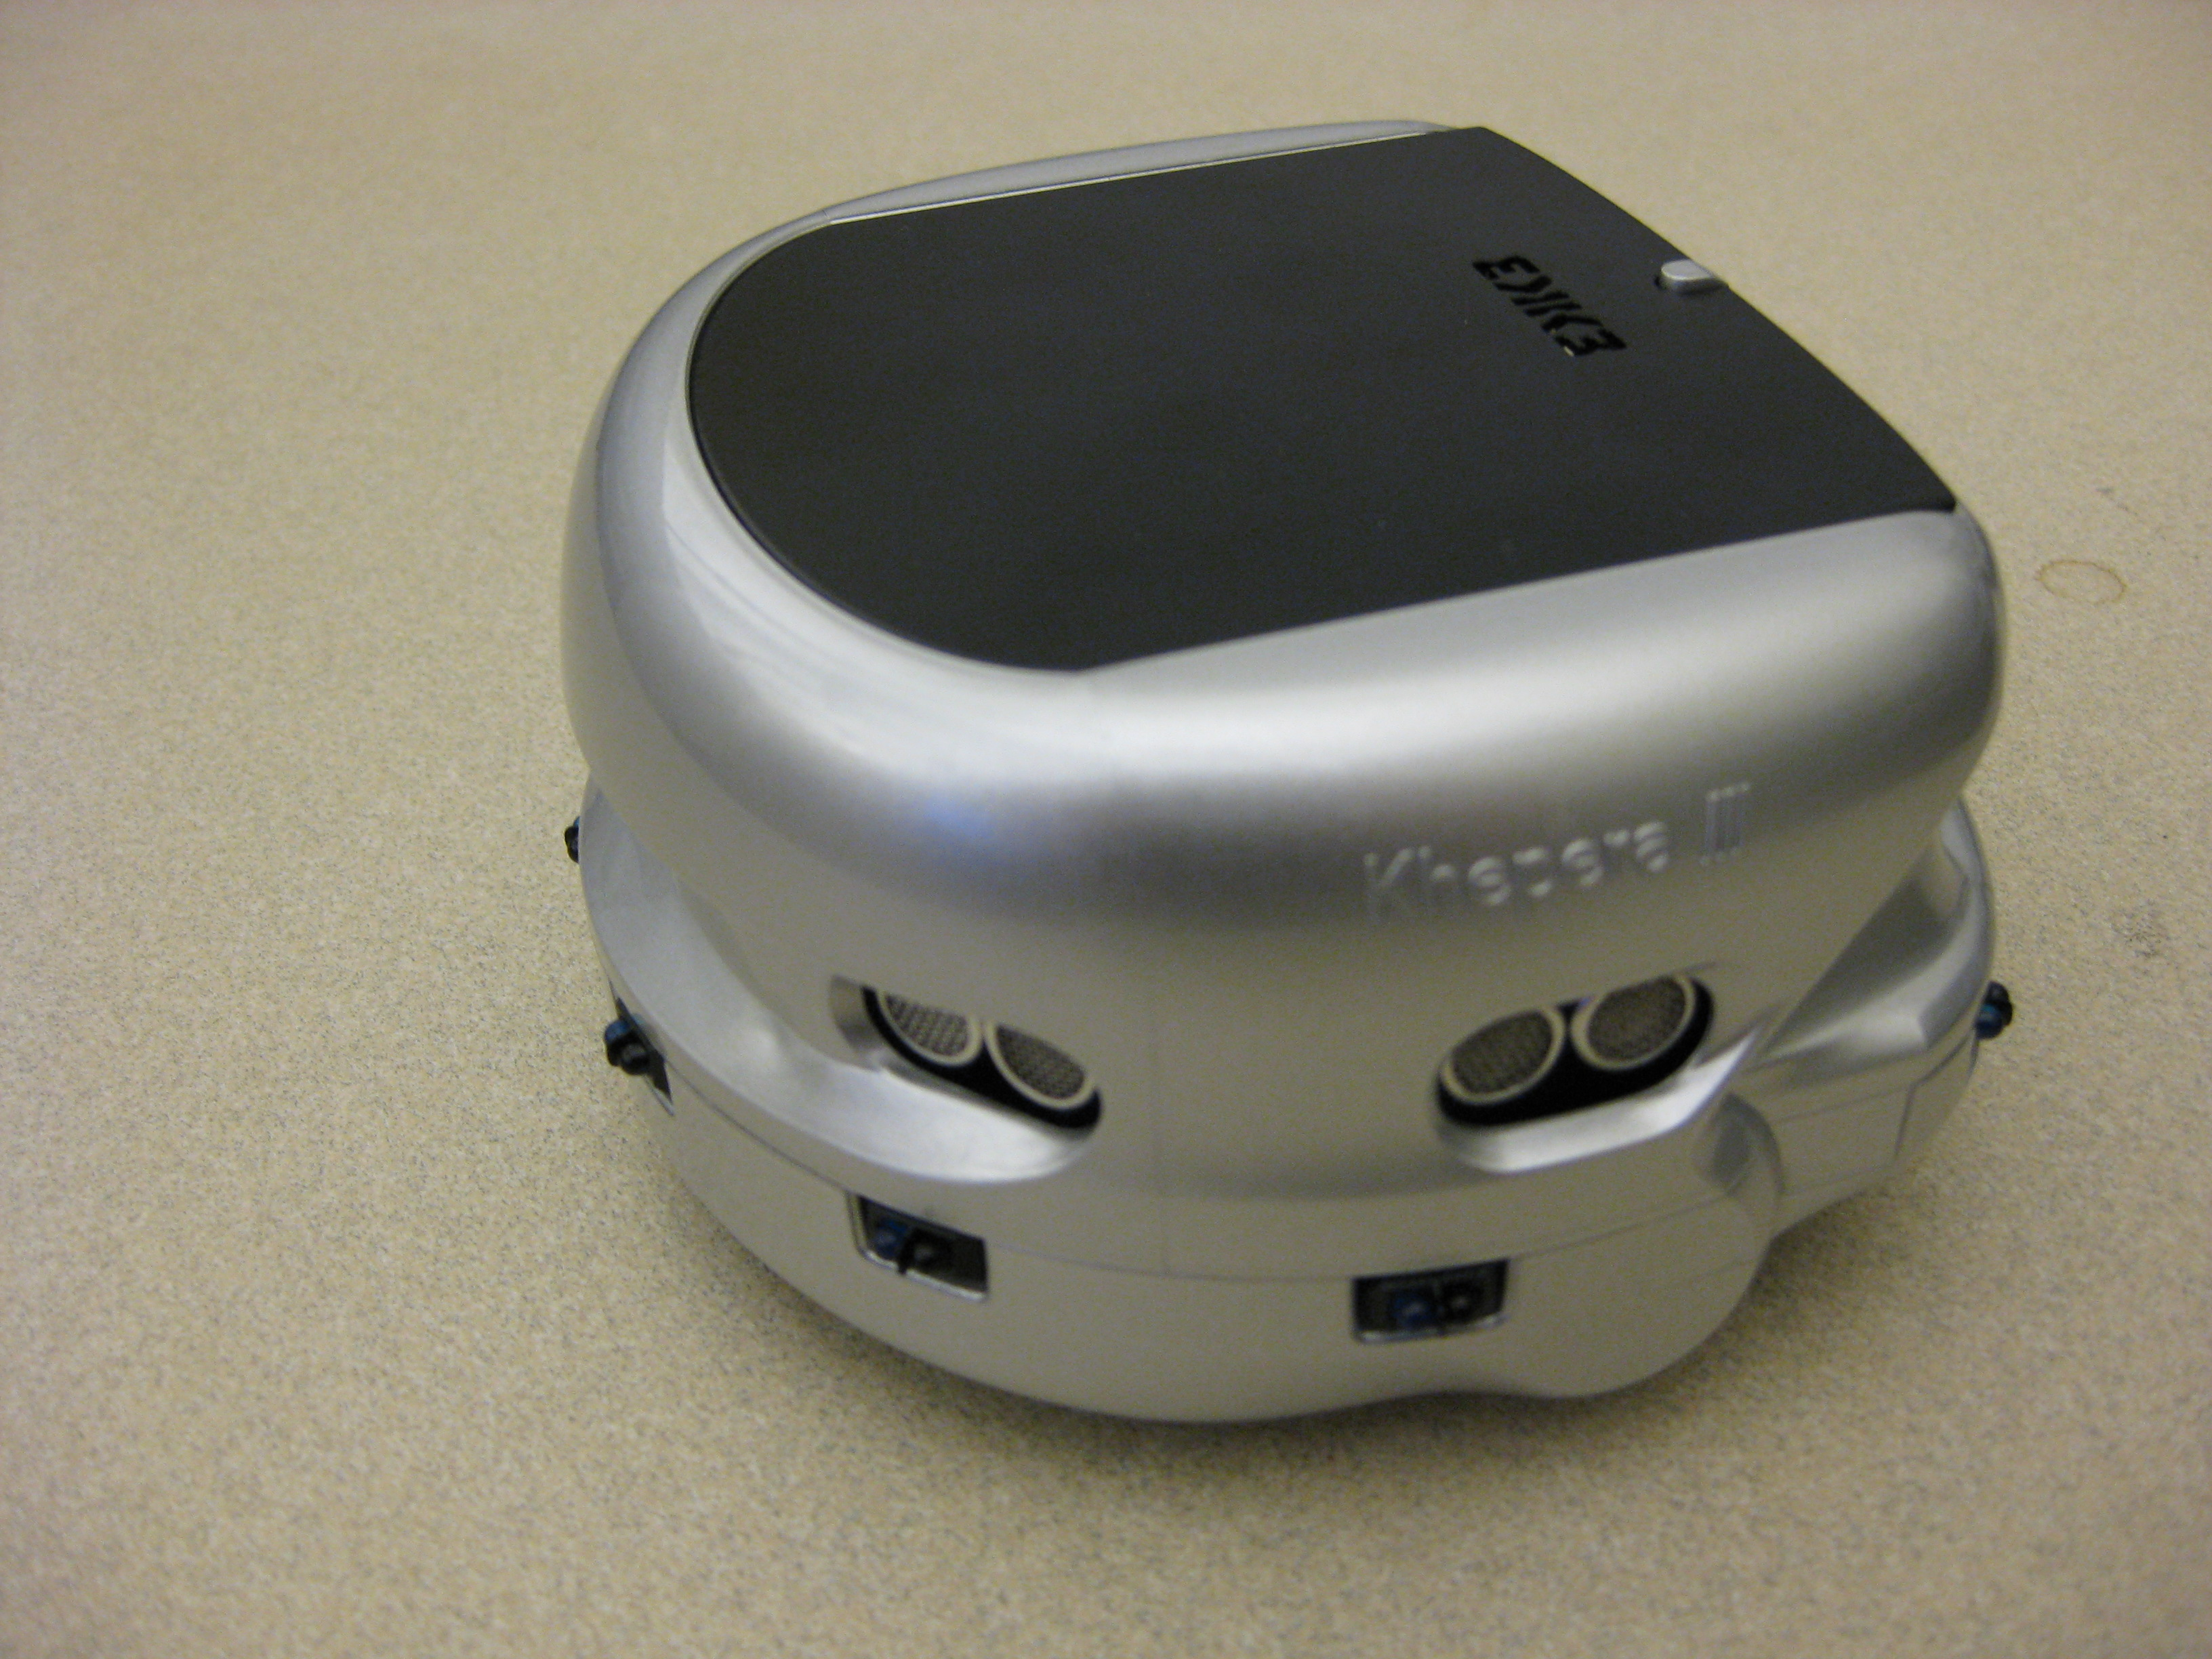
\includegraphics[trim= 8cm 0cm 0cm 0cm,clip,
scale=0.14]{Figuras/Khepera_III_robot}
		\subcaption{Robô Khepera 3}
	  	\label{fig:test1}
	\end{subfigure}
	~
	\begin{subfigure}[b]{0.49\textwidth}%
		\centering
		% fbox{}
		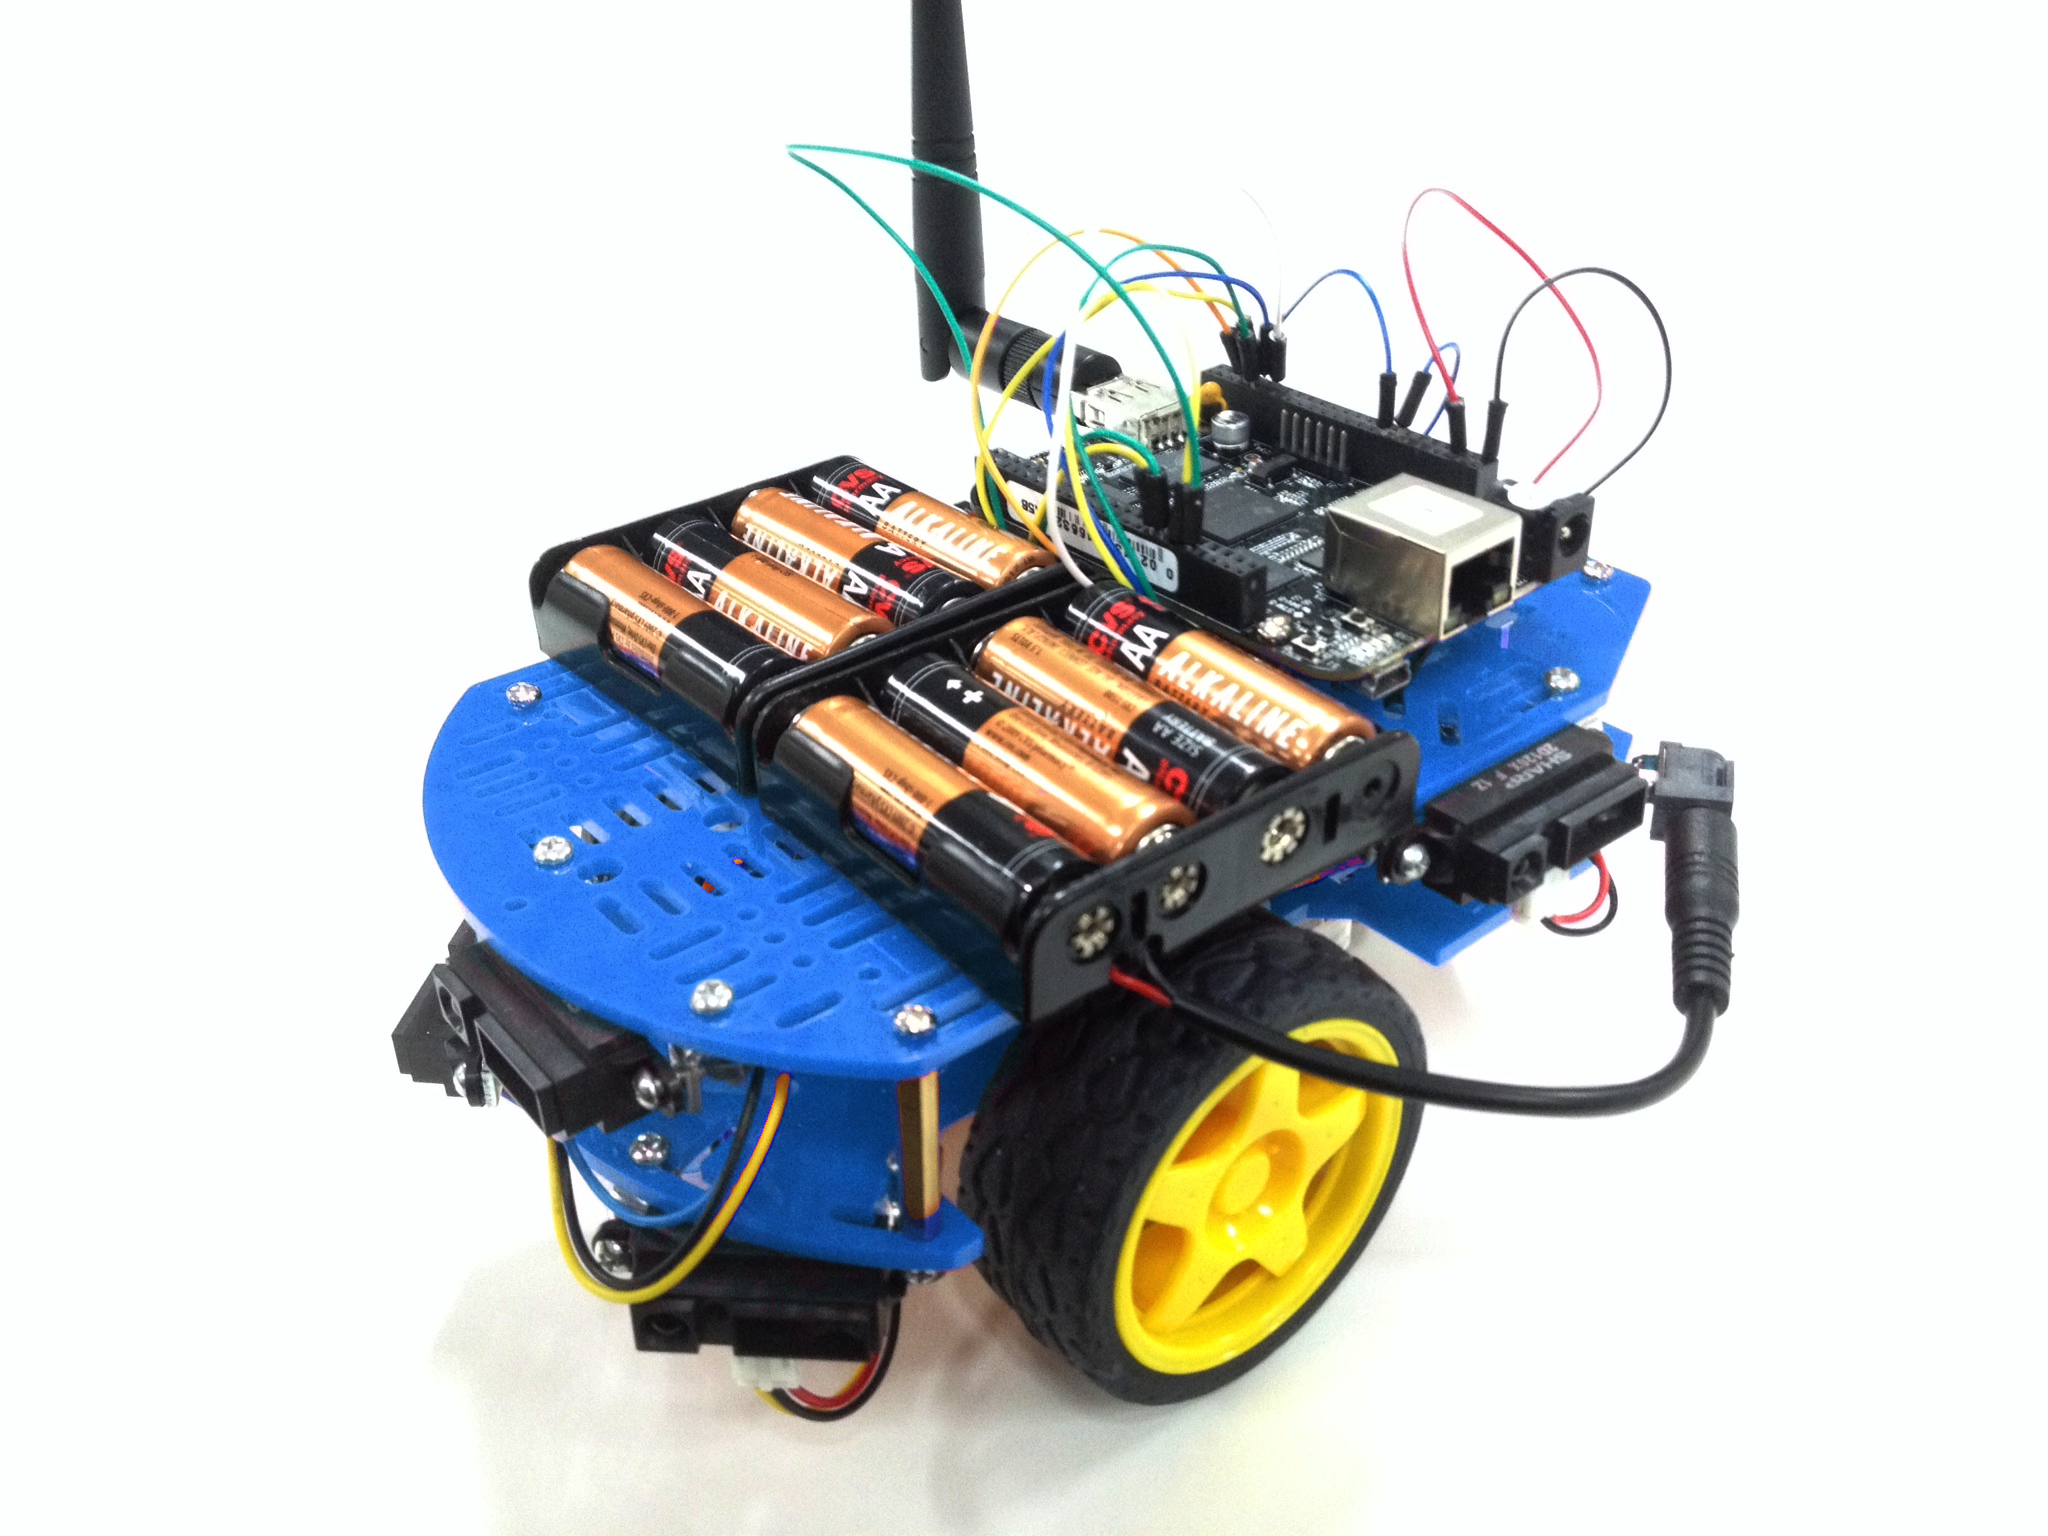
\includegraphics[trim={6cm 0cm 3cm 0cm},clip,
scale=0.09]{Figuras/quickbot-blue}
		\subcaption{Robô QuickBot}
	  	\label{fig:test2}
	\end{subfigure}
	
	\textbf{Fonte: \citeonline{im:Khepera}, \citeonline{im:QuickBot_Blue}}
\end{figure}


%		\begin{figure}[!htb]
%			\centering
%			\caption{Robôs Khepera e QuickBot fisicamente e em simulação}
%			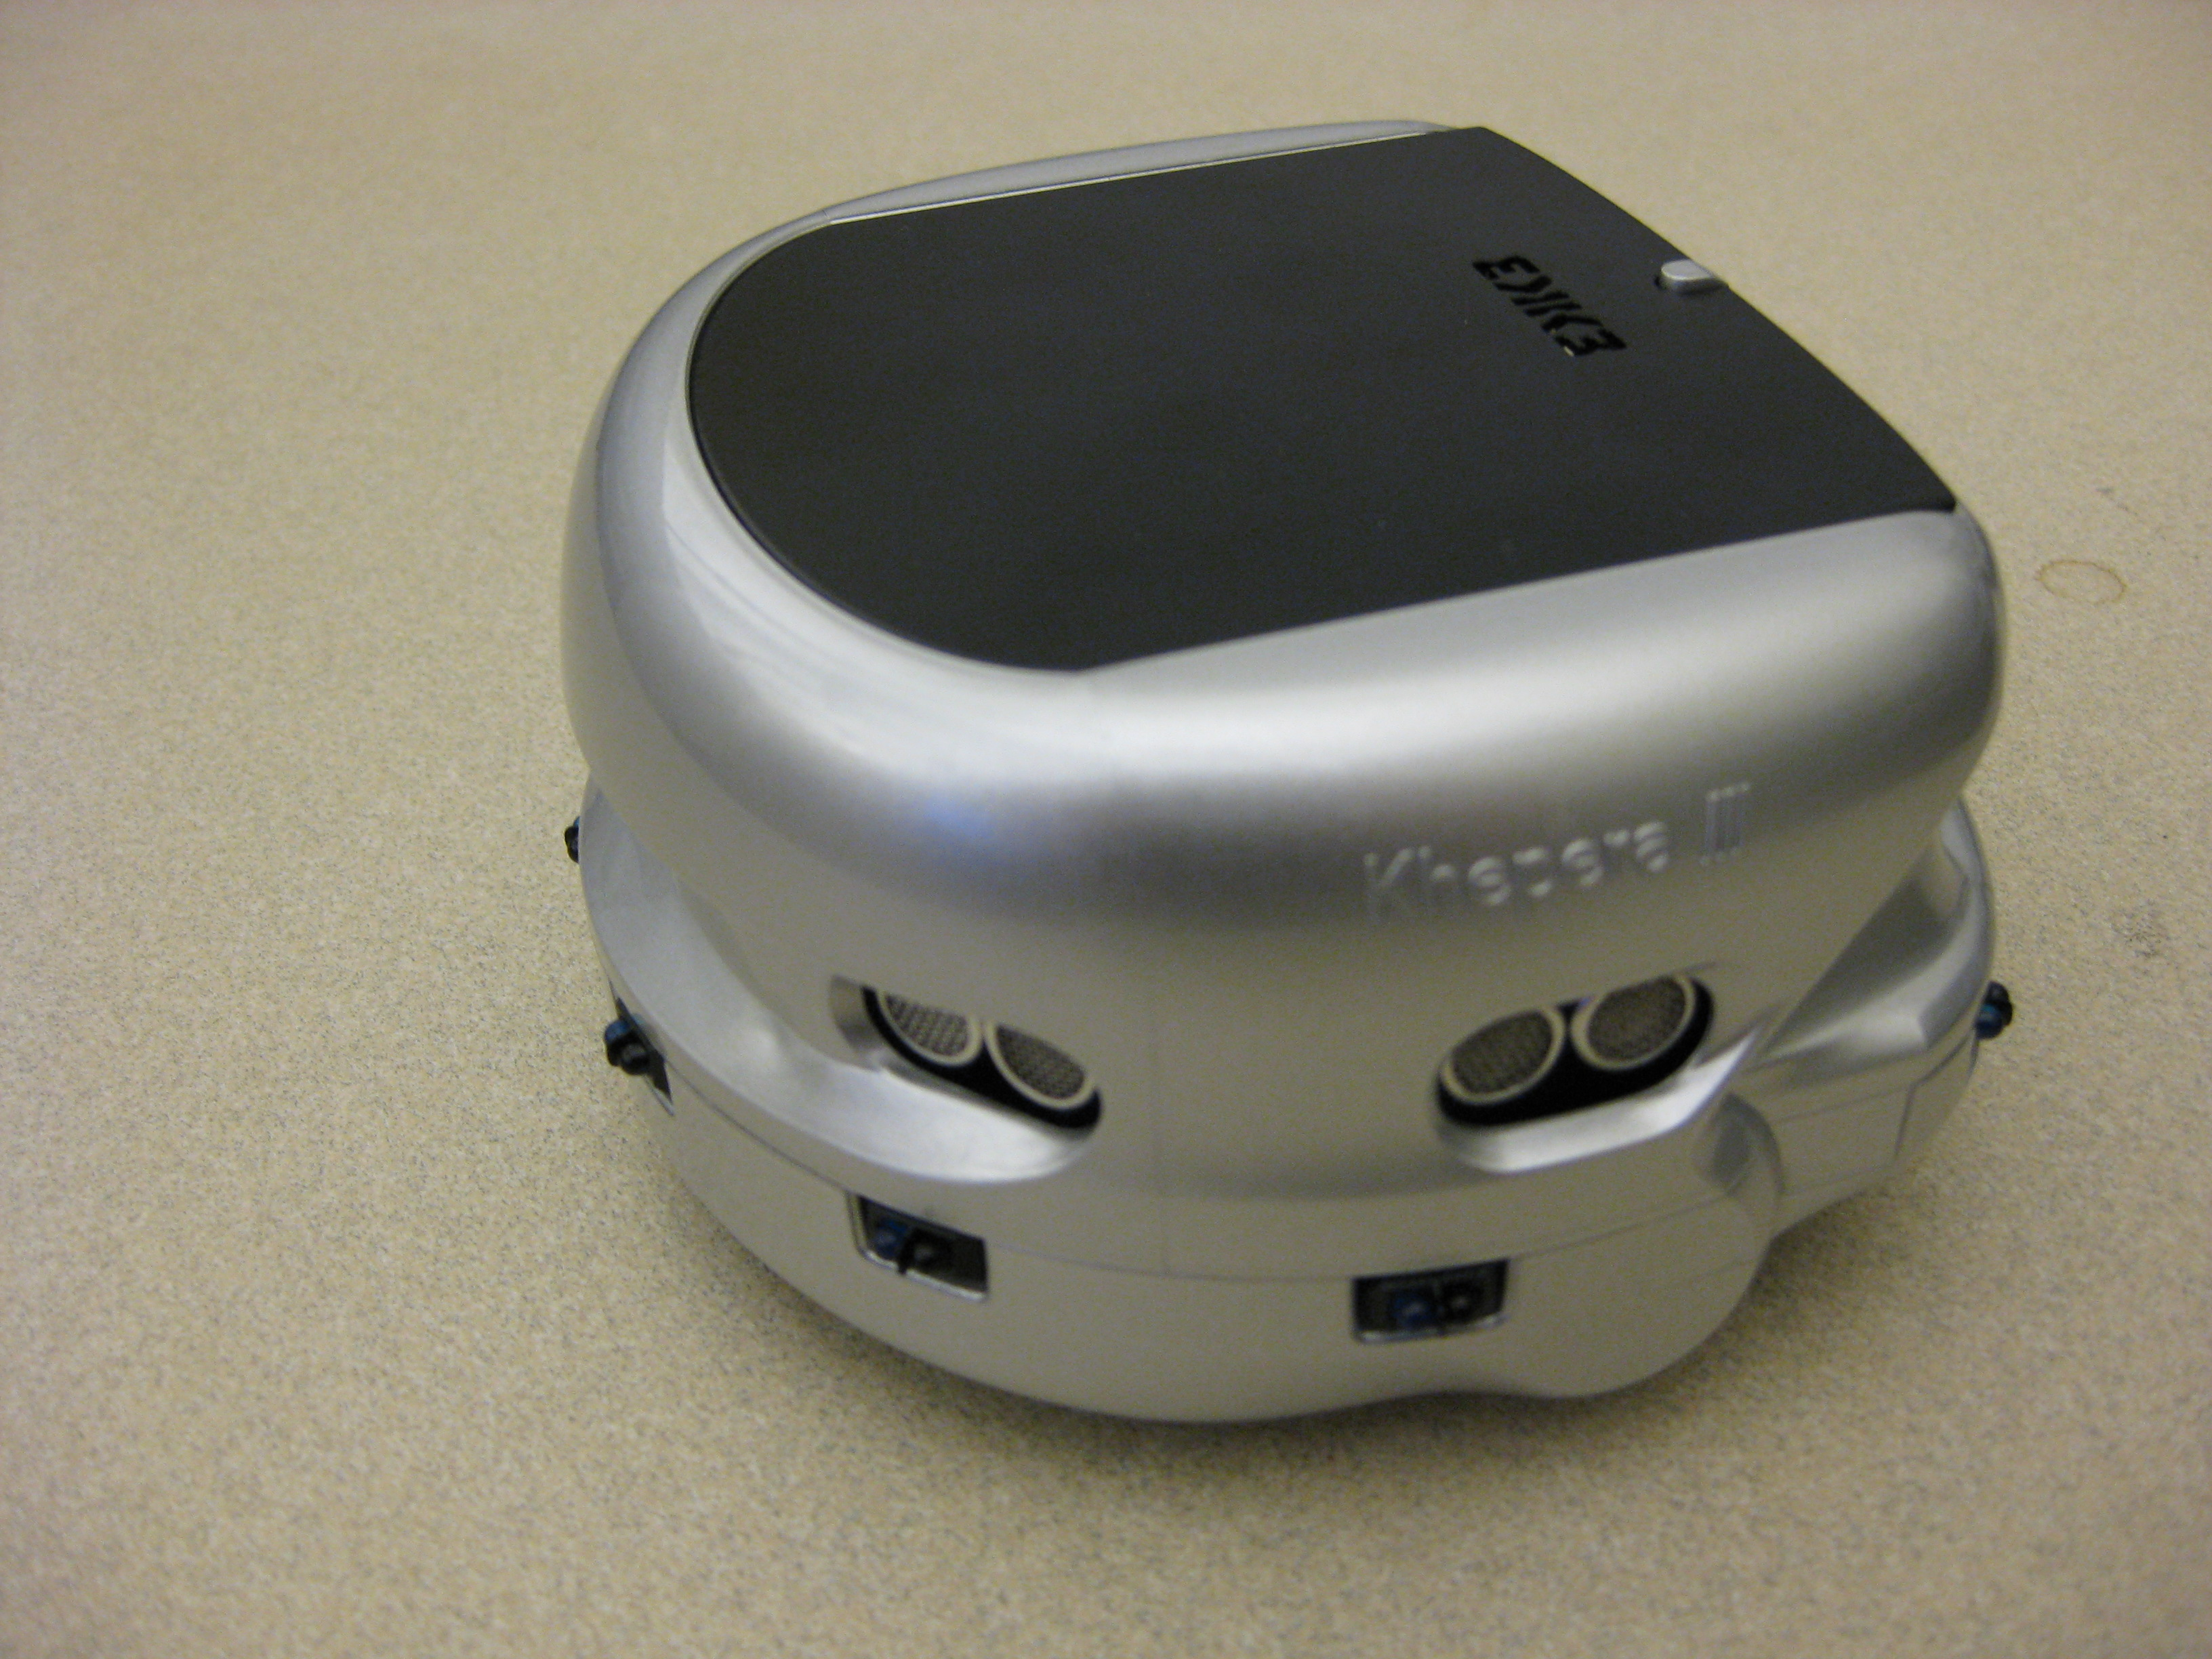
\includegraphics[trim={0cm 0cm 0cm 0cm},clip,
%scale=0.35]{Figuras/Khepera_III_robot}
%			%\vspace{-0.4cm}
%			\label{fig:RobosESim}
%		\end{figure}

%		\begin{figure}[!htb]
%			\centering			
%			\caption{Robôs Khepera e QuickBot fisicamente e em simulação}
%			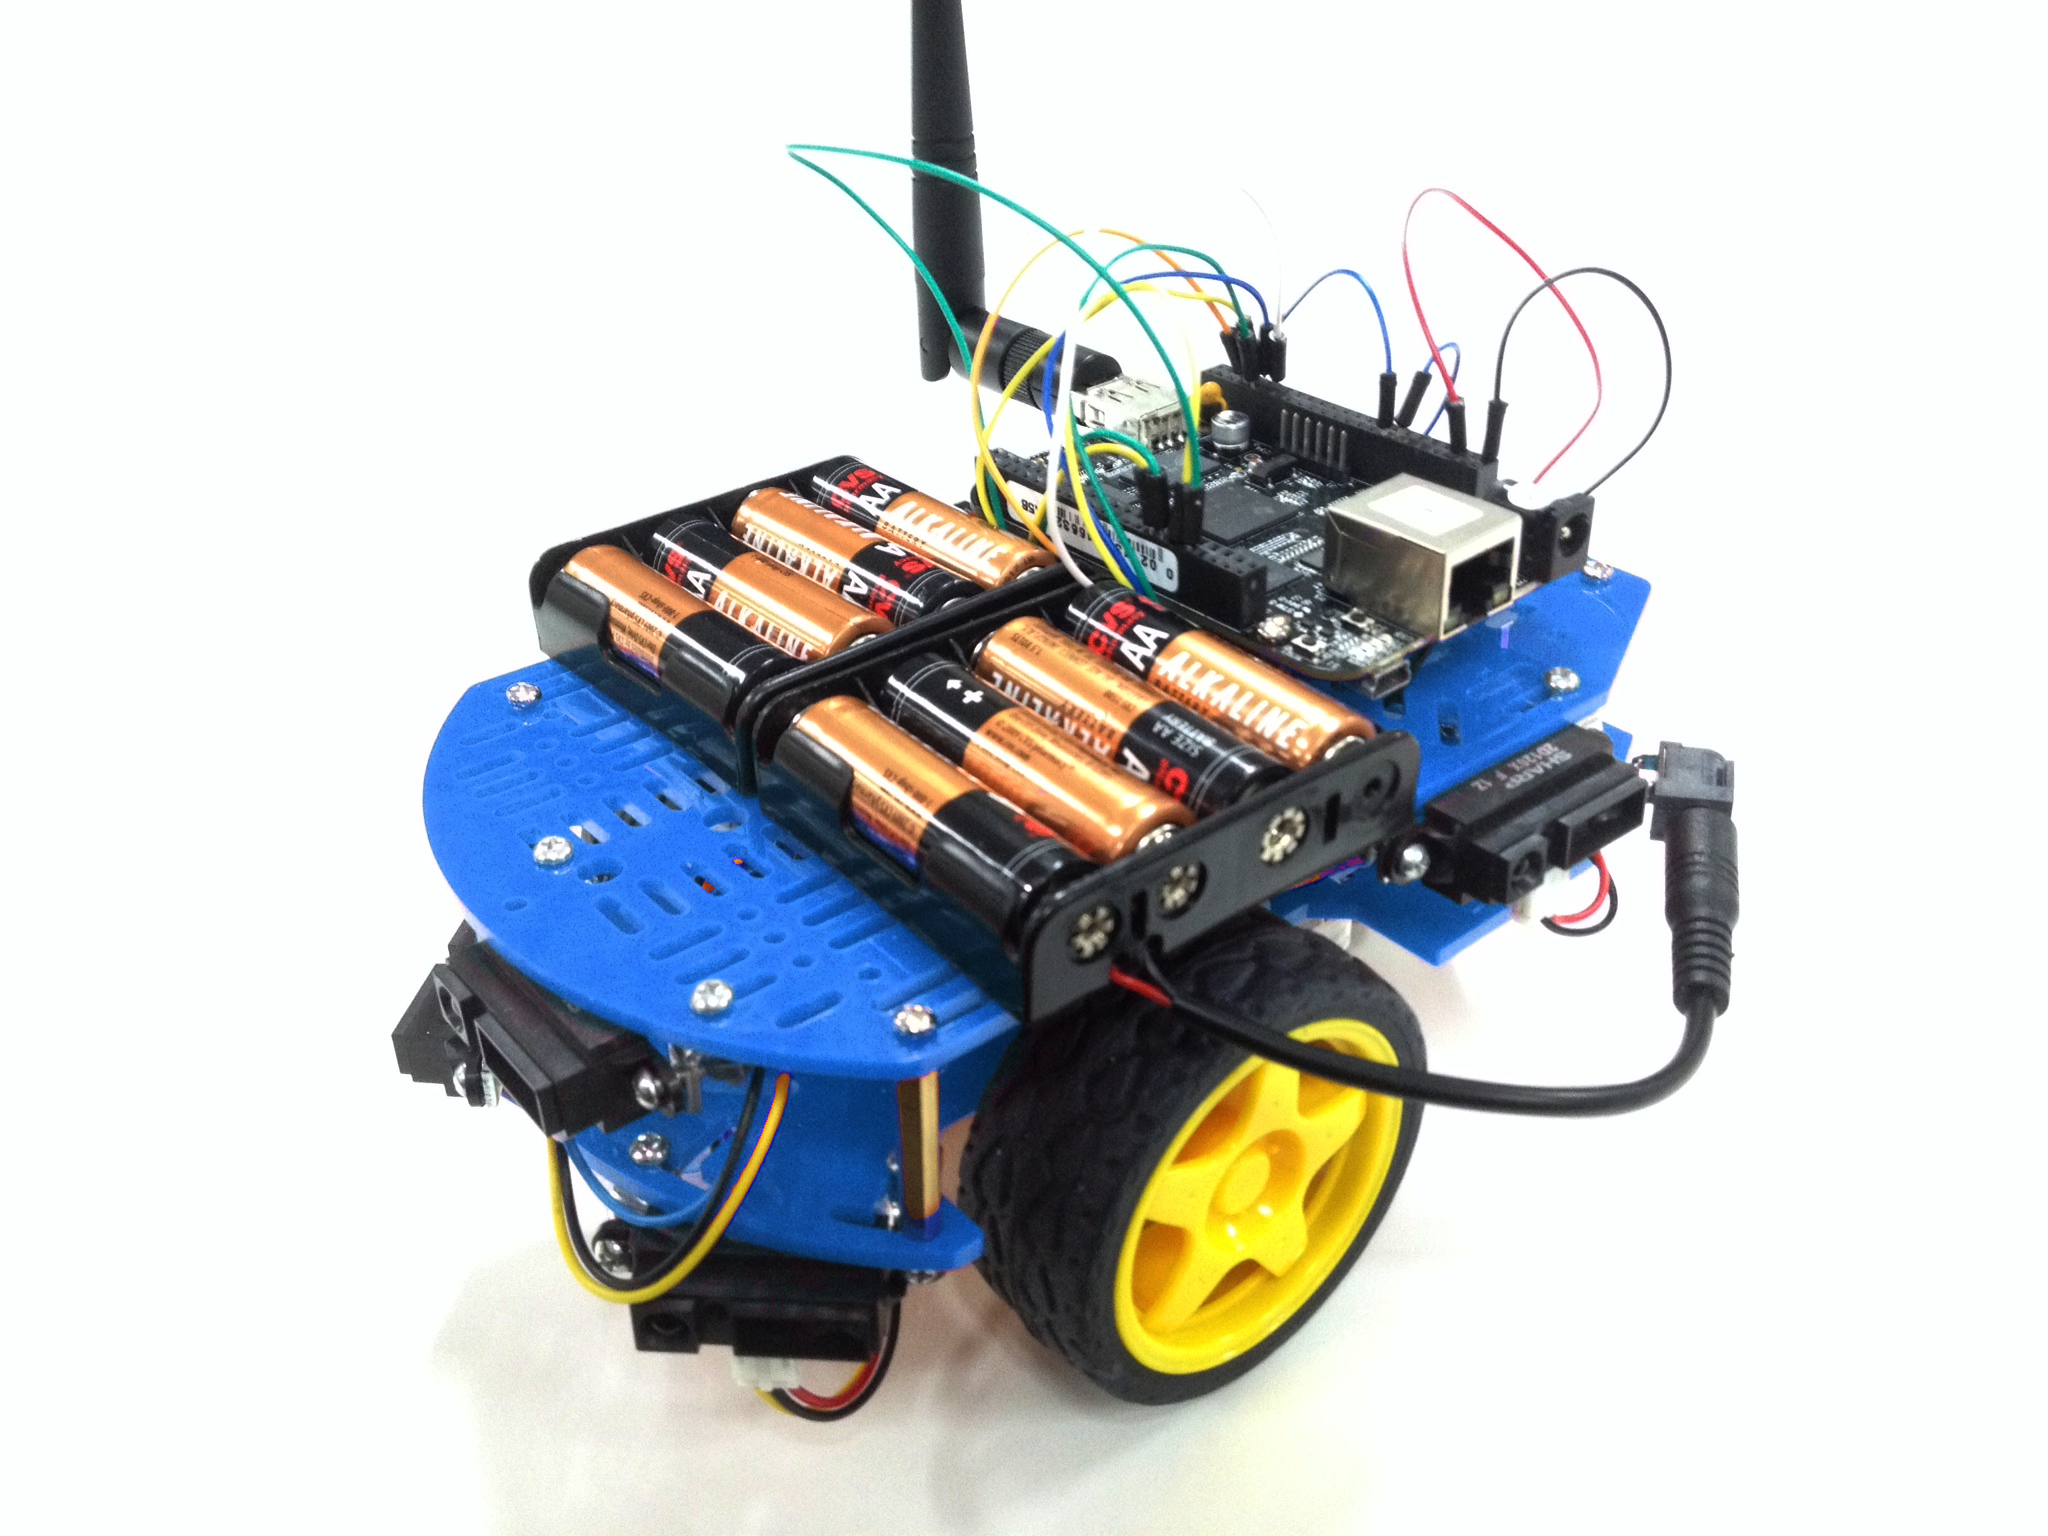
\includegraphics[trim={0cm 0cm 0cm 0cm},clip,
%scale=0.25]{Figuras/quickbot-blue}
%			%\vspace{-0.4cm}
%			\label{fig:RobosESim}
%		\end{figure}

%		\begin{figure}[!htb]
%			\centering
%			\caption{Robôs Khepera e QuickBot fisicamente e em simulação}
%			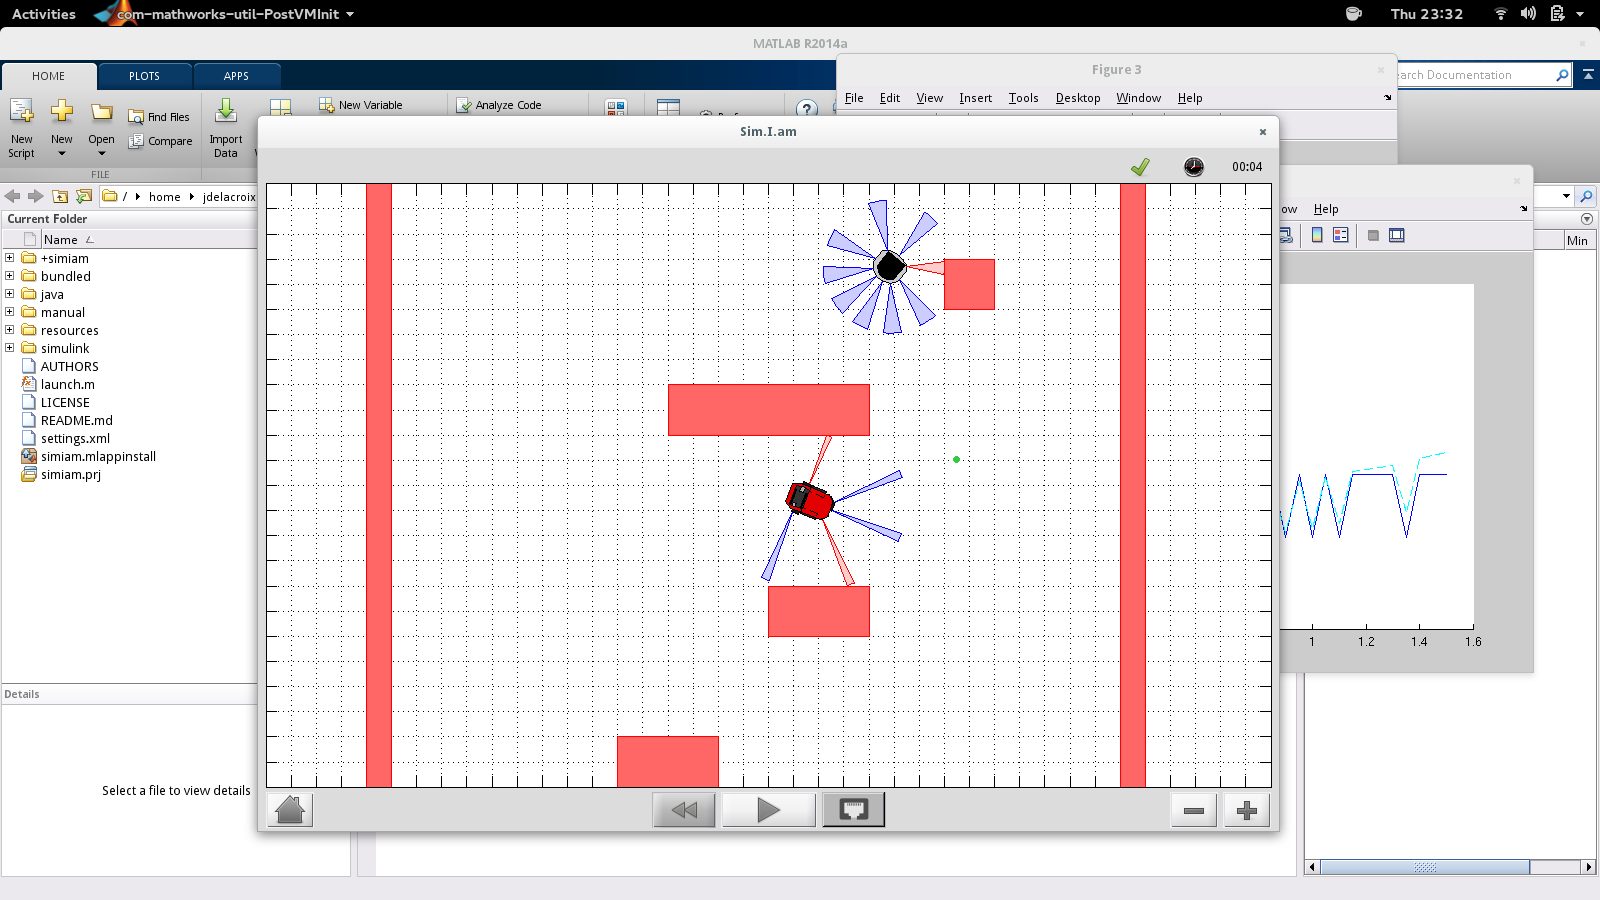
\includegraphics[trim={0cm 0cm 0cm 0cm},clip,
%scale=0.25]{Figuras/simiam-screenshot}
%			%\vspace{-0.4cm}
%			\label{fig:RobosESim}
%		\end{figure}


%\begin{figure}
%\begin{minipage}[c][11cm][t]{.5\textwidth}
%  \vspace*{\fill}
%  \centering
%  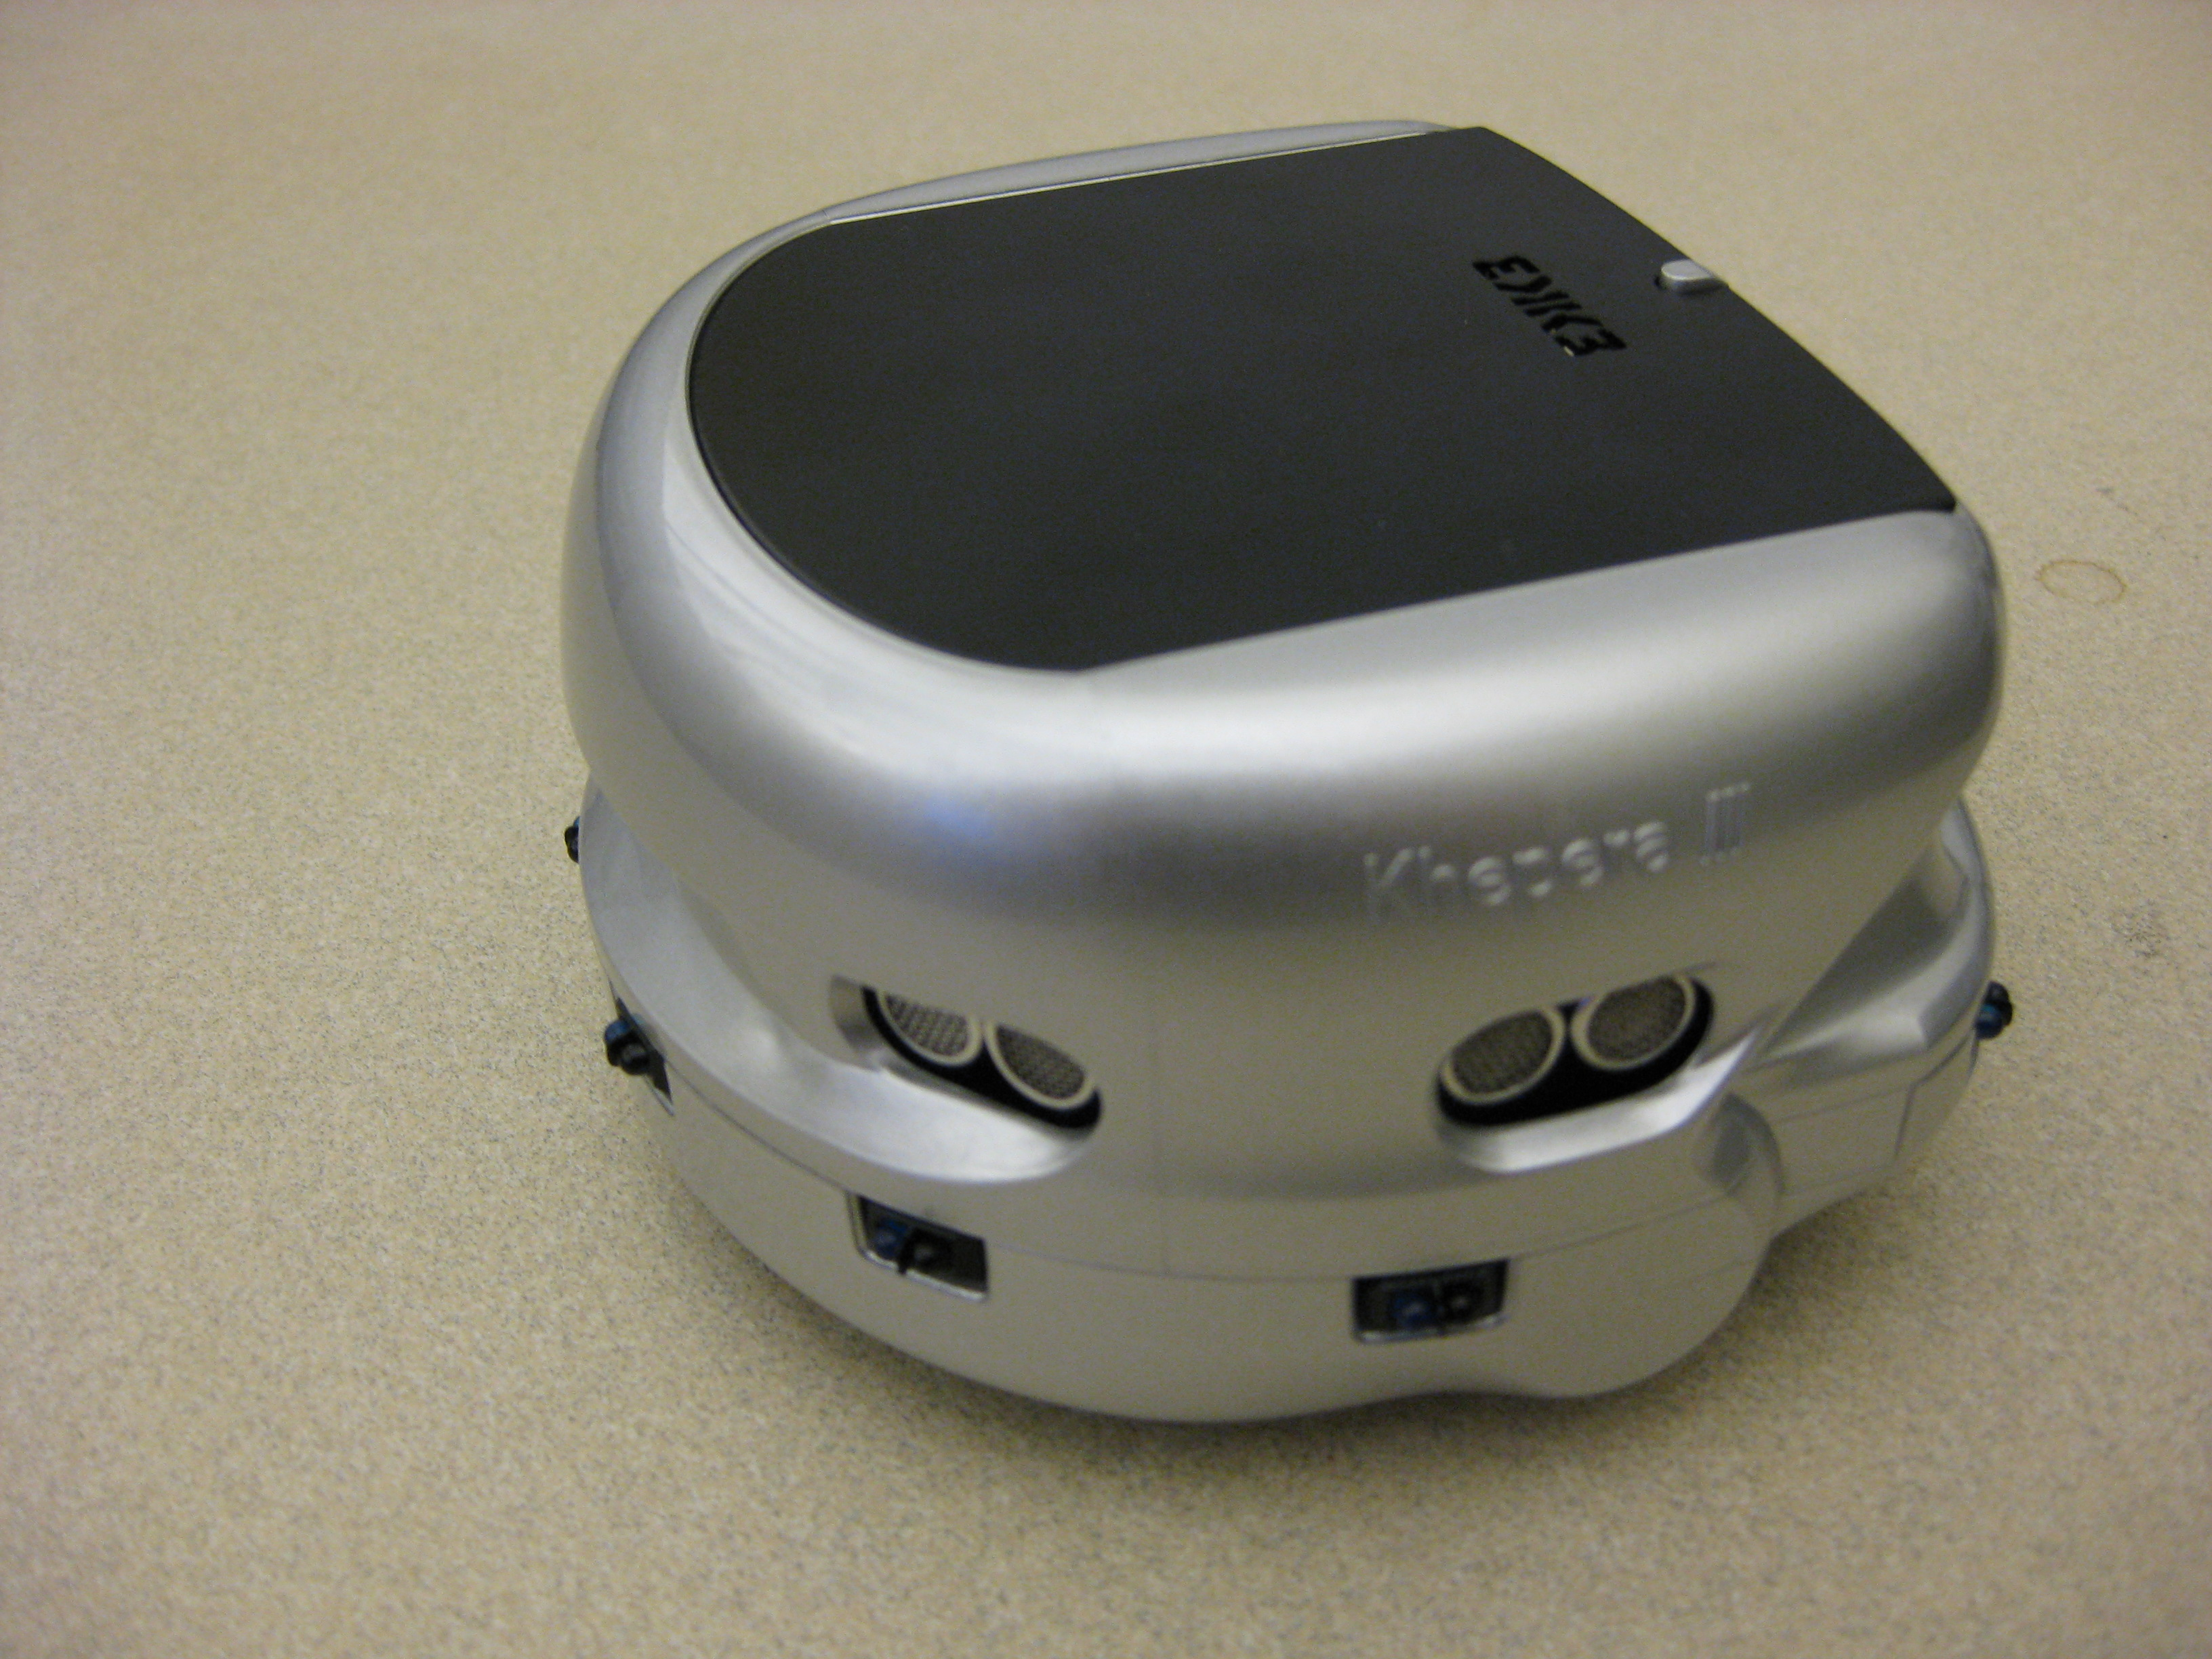
\includegraphics[width=5cm,height=4.5cm]{Figuras/Khepera_III_robot}
%  \subcaption{Robô Khepera}
%  \label{fig:test2}\par\vfill
%  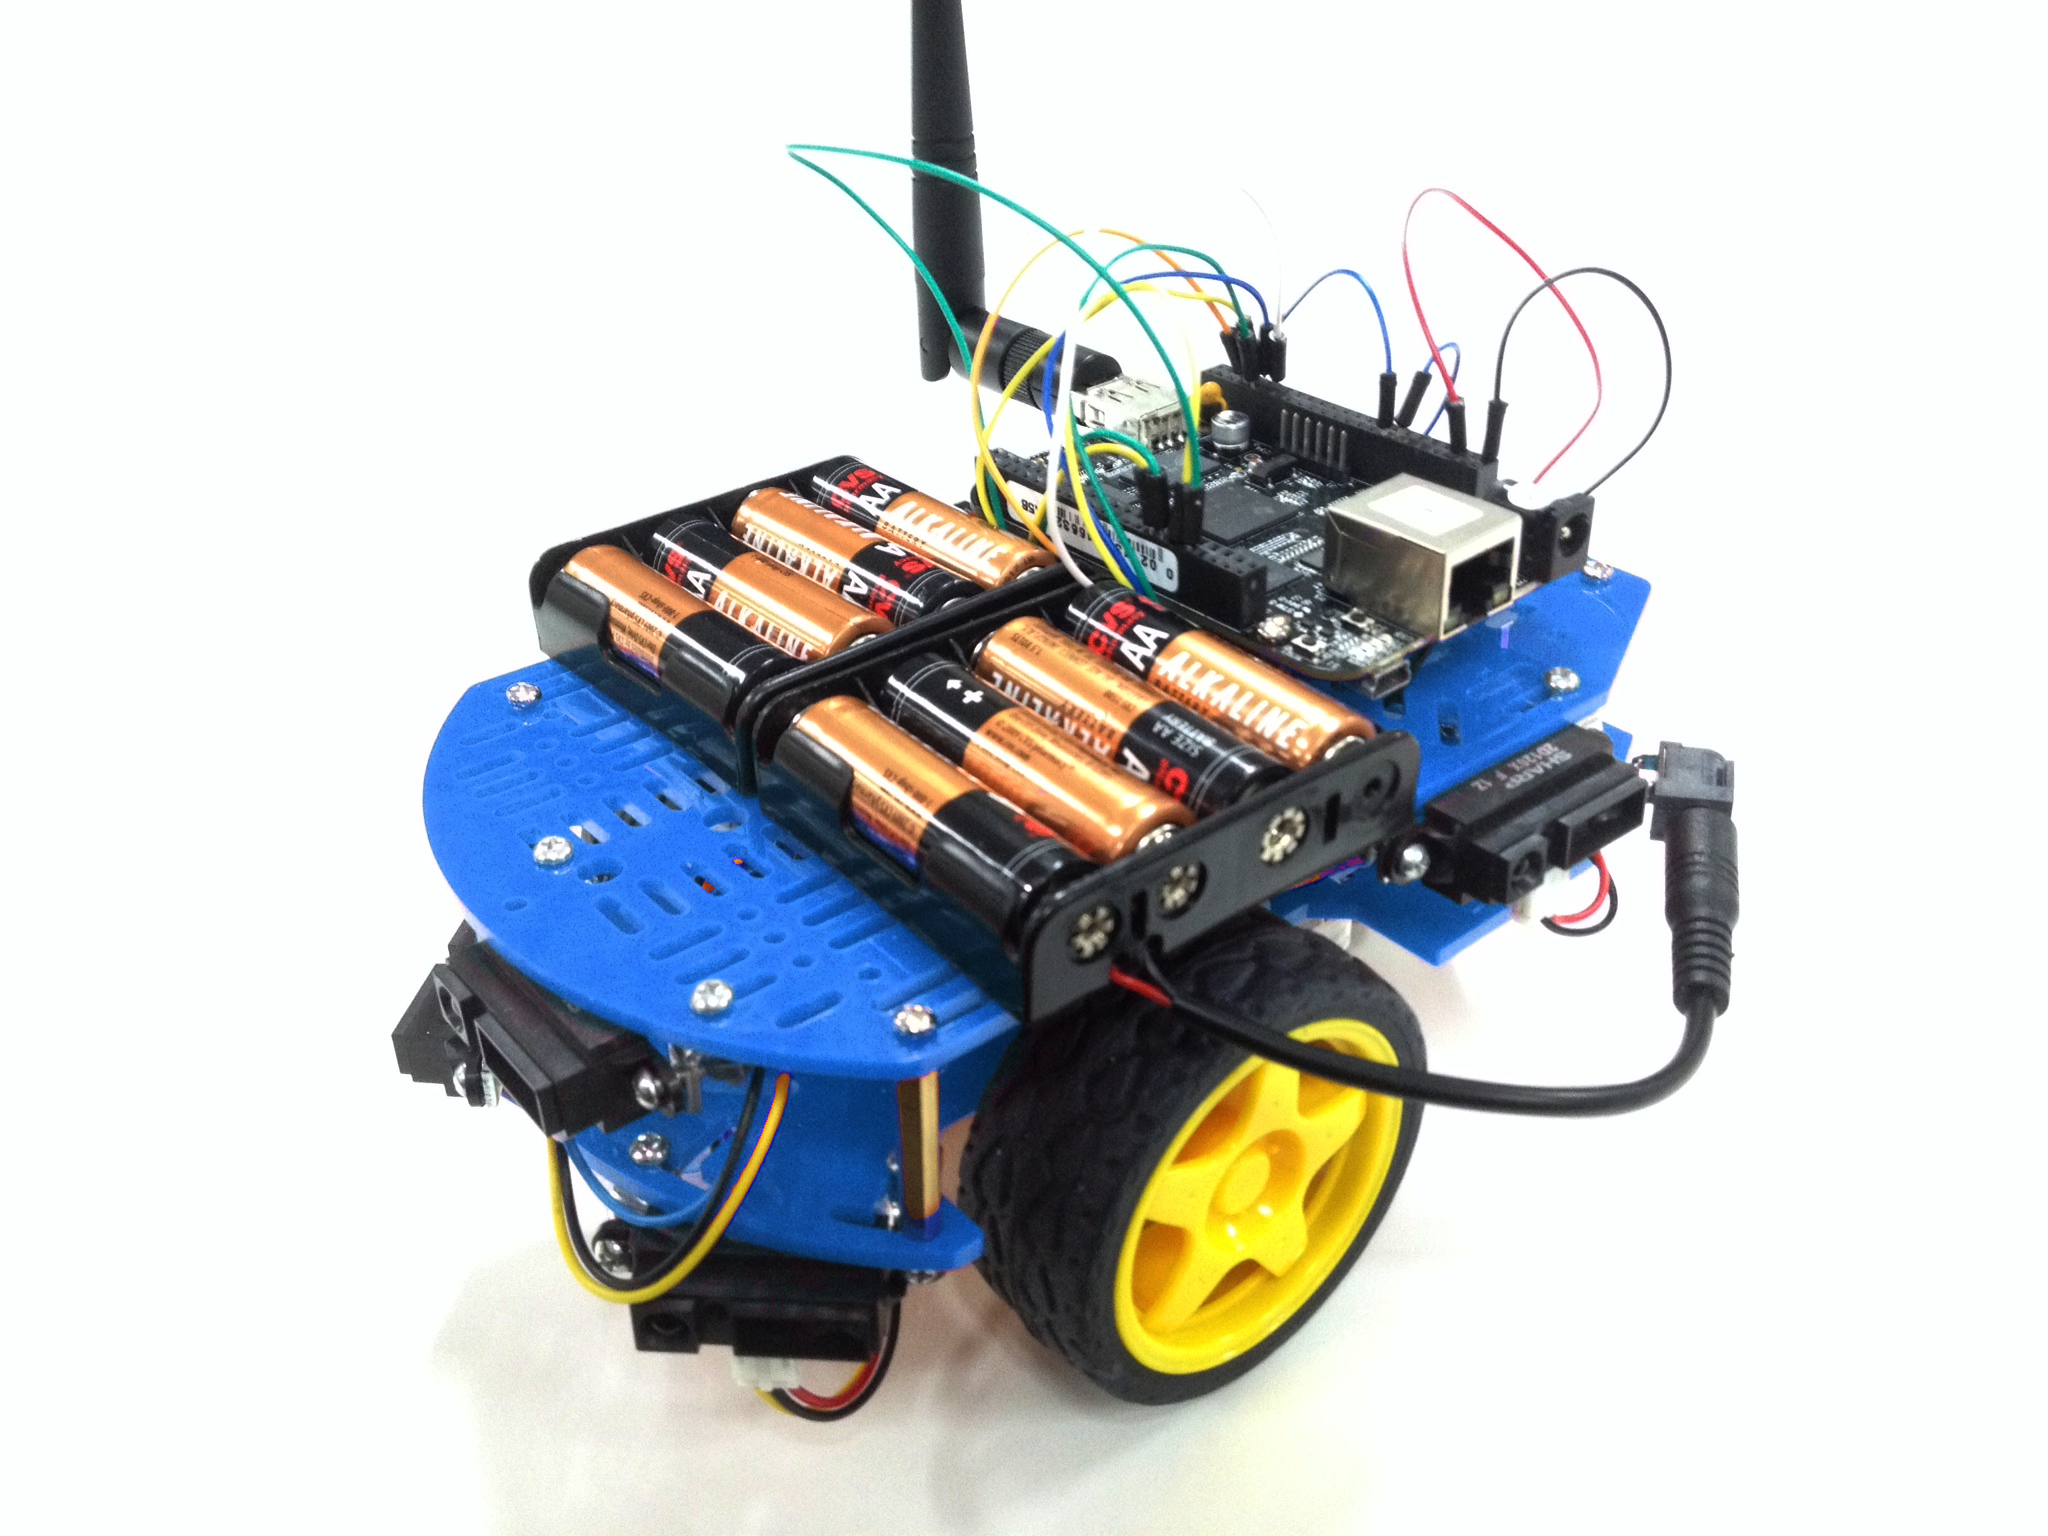
\includegraphics[width=5cm,height=4.5cm]{Figuras/quickbot-blue}
%  \subcaption{Robô QuickBot}
%  \label{fig:test3}
%\end{minipage}
%\begin{minipage}[c][11cm][t]{.5\textwidth}
%  \vspace*{\fill}
%  \centering
%  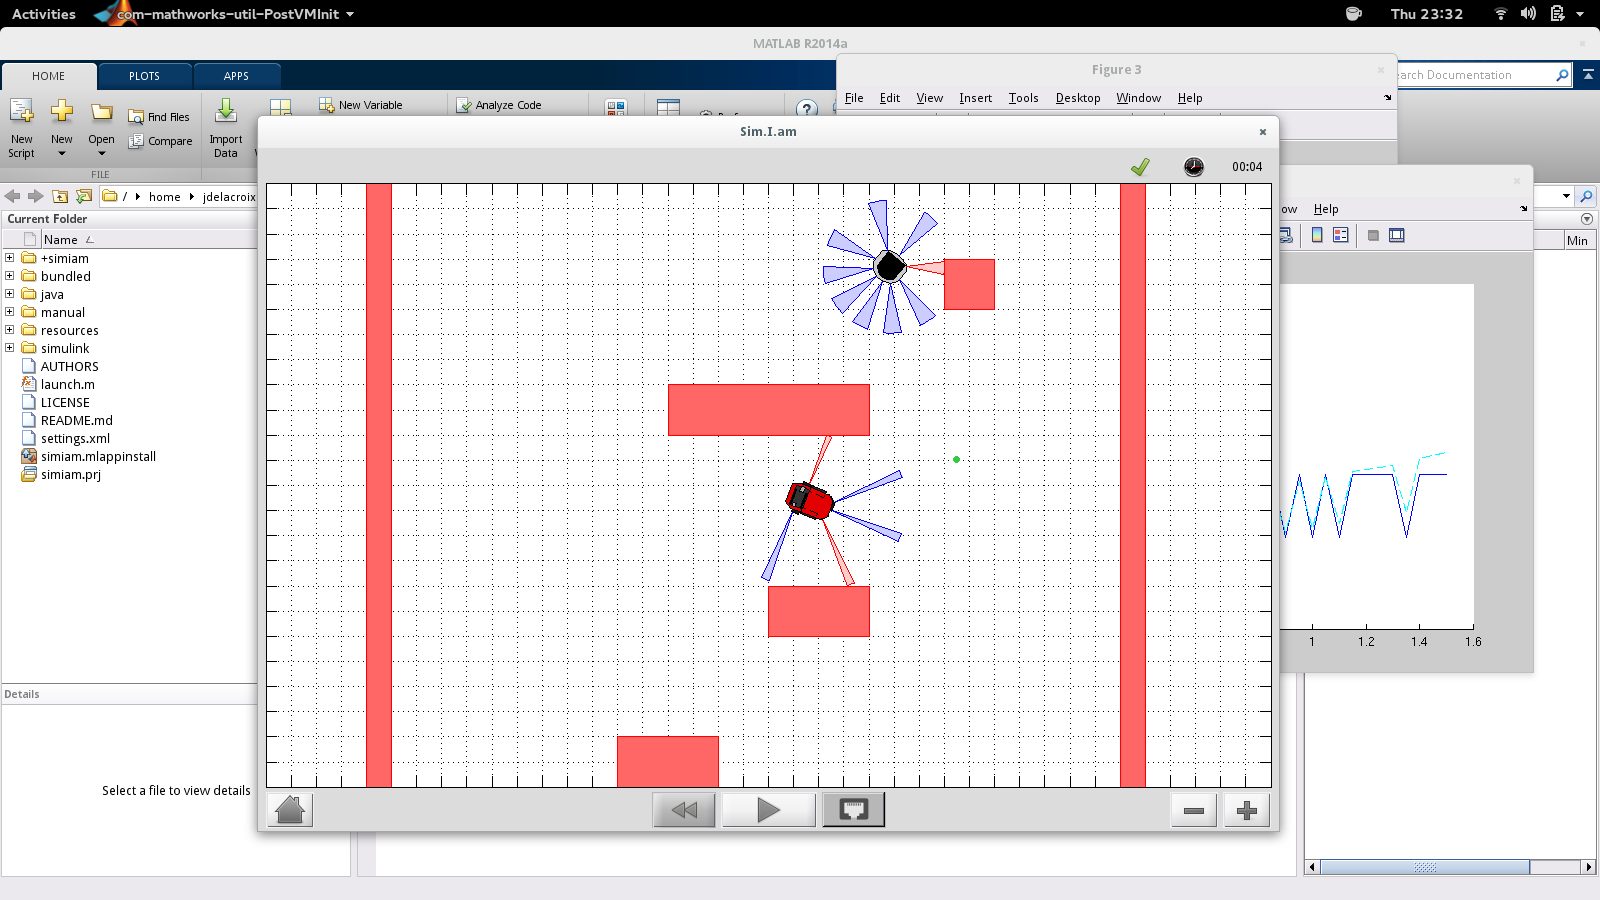
\includegraphics[width=5cm,height=10cm]{Figuras/simiam-screenshot}
%  \subcaption{Simulador Simiam}
%  \label{fig:test1}
%\end{minipage}%
%\end{figure}

\begin{figure}[ht]
\centering
\caption{Robôs Khepera 3 e QuickBot em simulação}
\label{fig:RobosEmSimulador}
		\centering
		% fbox{}
		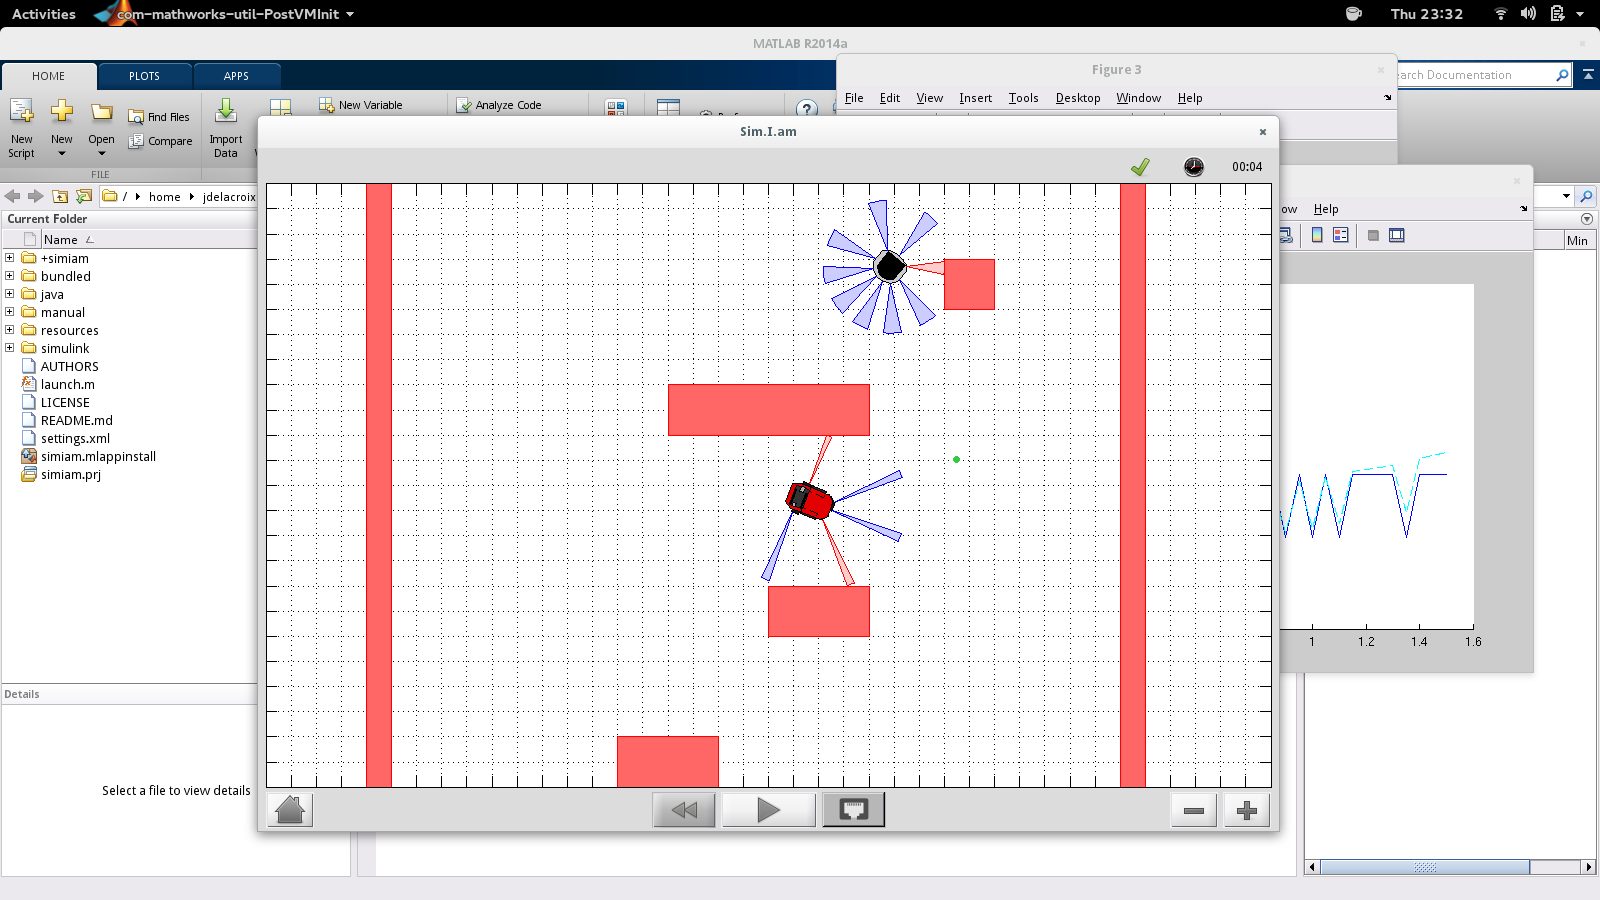
\includegraphics[trim={0cm 0cm 0cm 0cm},clip,
scale=0.24]{Figuras/simiam-screenshot}
	
	\textbf{Fonte: \citeonline{im:Simiam}}
\end{figure}

O Simiam é implementado como um aplicativo Matlab. Possui uma interface
gráfica intuitiva e uma arquitetura interna simples, facilmente customizável. As
subseções a seguir apresentam os pacotes mais importantes, bem como as
principais classes que os compõem e chama atenção para as alterações necessárias
a fim de tornar a simulação coerente com o presente trabalho.

	\subsection{Pacote ``ui''}
	
	O pacote ``ui'' é responsável pela interface gráfica do simulador. A classe
	``AppWindow'' possui um método construtor que inicializa atributos e o
	método ``load\_ui'' que invoca o método ``create\_layout", responsável por
	criar o leiaute da interface.
	
	O botão start, criado pelo método anterior é tratado por ``ui\_button\_start".
	Esta é a função principal reponsável por criar o ambiente de simulação
	(definido no arquivo ``settings.xml''), inserir um ou mais robôs e iniciar a
	simulação.
	
	Alterações mínimas foram efetuadas nesta etapa. Foram adicionados comandos para
	maximizar a janela do simulador e para ajustar o ``zoom'' de modo a permitir uma
	visão panorâmica de todo o ambiente de simulação. O arquivo de configuração
	``settings.xml'' foi alterado a fim de ajustar o ``tamanho do mundo'' ao
	tamanho da	tela.
	
	\subsection{Pacote ``simulator''}
	
	O pacote ``simulator'' realiza de fato a simulação. A classe ``World'' é
	responsável por extrair informações do arquivo ``.xml'', como quantidade e
	localização inicial de robôs e obstáculos, armazenado em estruturas de dados.
	A classe ``Simulator'' atualiza a simulação na janela, enquanto a
	classe ``Physics'' é responsável por detectar colisões de robôs com obstáculos
	e entre si. 
	
	As alterações neste pacote foram todas na classe ``Simulator'', no intuito
	de possibilitar a captura da simulação em video ``.mp4" ou ``.gif". Apesar de
	não ser uma alteração fundamental para a etapa de execução do trabalho, é
	necessária para a apresentação. Não foi criado um botão na interface para
	especificar ao simulador a captura em video. Assim, é necessário, no
	construtor da classe Simulator, atribuir valor verdadeiro aos atributos
	``gravarvideo'' e/ou ``gravargif". 
	
	\subsection{Pacote ``robot''}
	
	O pacote ``robot'' define um ou mais robôs passíveis de serem instanciados. A
	classe ``QuickBot'' estabelece parâmetros físicos, tais como informações
	geométricas, posicionamento dos sensores no corpo do robô e estabelece
	limitações, como velocidades de saturação e zona morta dos motores. Além de
	instanciar objetos das classes ``DifferentialDrive'', ``ProximitySensor'' e
	``WheelEncoder'', ``QuickBot'' extende a classe ``Robot''. 
	
	A classe ``DifferentialDrive" implementa a ``dinâmica'' dos modelos de
	acionamento diferencial e uniciclo. Com os métodos ``uni\_to\_diff'' e ``diff\_to\_uni'', a
	equivalência entre modelo apresentada na Equação \ref{eq:vw_to_diff} é
	estabelecida no espaço de simulação. 

	A classe ``ProximitySensor'' estabelece características do sensor infravermelho
	usado no QuickBot, tais como distâncias mínimas e máximas, espalhamento, localização e
	direção em relação ao corpo do robô e adiciona um ruído gaussiano.
	``WheelEncoder'', similarmente, estabelece características do \textit{encoder}.
	
	As alterações nesta etapa foram no intuito de incluir o robô deste trabalho
	no Simiam. O arquivo ``settings.xml'' deve determinar que um objeto (robô) da
	nova classe criada seja instanciado, ao invés do objeto da classe QuickBot.
	
	\subsection{Pacote ``controller''}
	
	O pacote ``controller'' é responsável pela implementação de todos os
	controladores e supervisores dos robôs implementados. A classe ``Supervisor'' é
	extendida para obter o controlador supervisório de cada robô a ser simulado.
	Para o QuickBot e Khepera 3, os respectivos supervisores são definidos pelas
	classes ``QBSupervisor'' e ``K3Supervisor''. Essas classes definem máquinas de
	estado, onde cada estado é associado a um controlador de variável contínua.
	Esses controladores, por sua vez, extendem a classe ``Controller'' e
	implementam os ``comportamentos'', ou modos, dos robôs.
	% Calculo de odometria está em QBSupervisor.
	
	As alterações neste pacote foram responsáveis pela inclusão de suporte a
	controladores \textit{Fuzzy}, além de adicionar o supervisório específico para
	o robô desenvolvido.
	 
\section{Montagem física do robô}

Os componentes físicos do robô podem ser vistos na Figura \ref{fig:RoboReal}.a e
o resultado após montagem está retratado na Figura \ref{fig:RoboReal}.b.

\begin{figure}[!ht]
\centering
\caption{Materiais e robô após montagem}
\label{fig:RoboReal}
	\begin{subfigure}[b]{0.49\textwidth}%
		\centering
		% fbox{}
		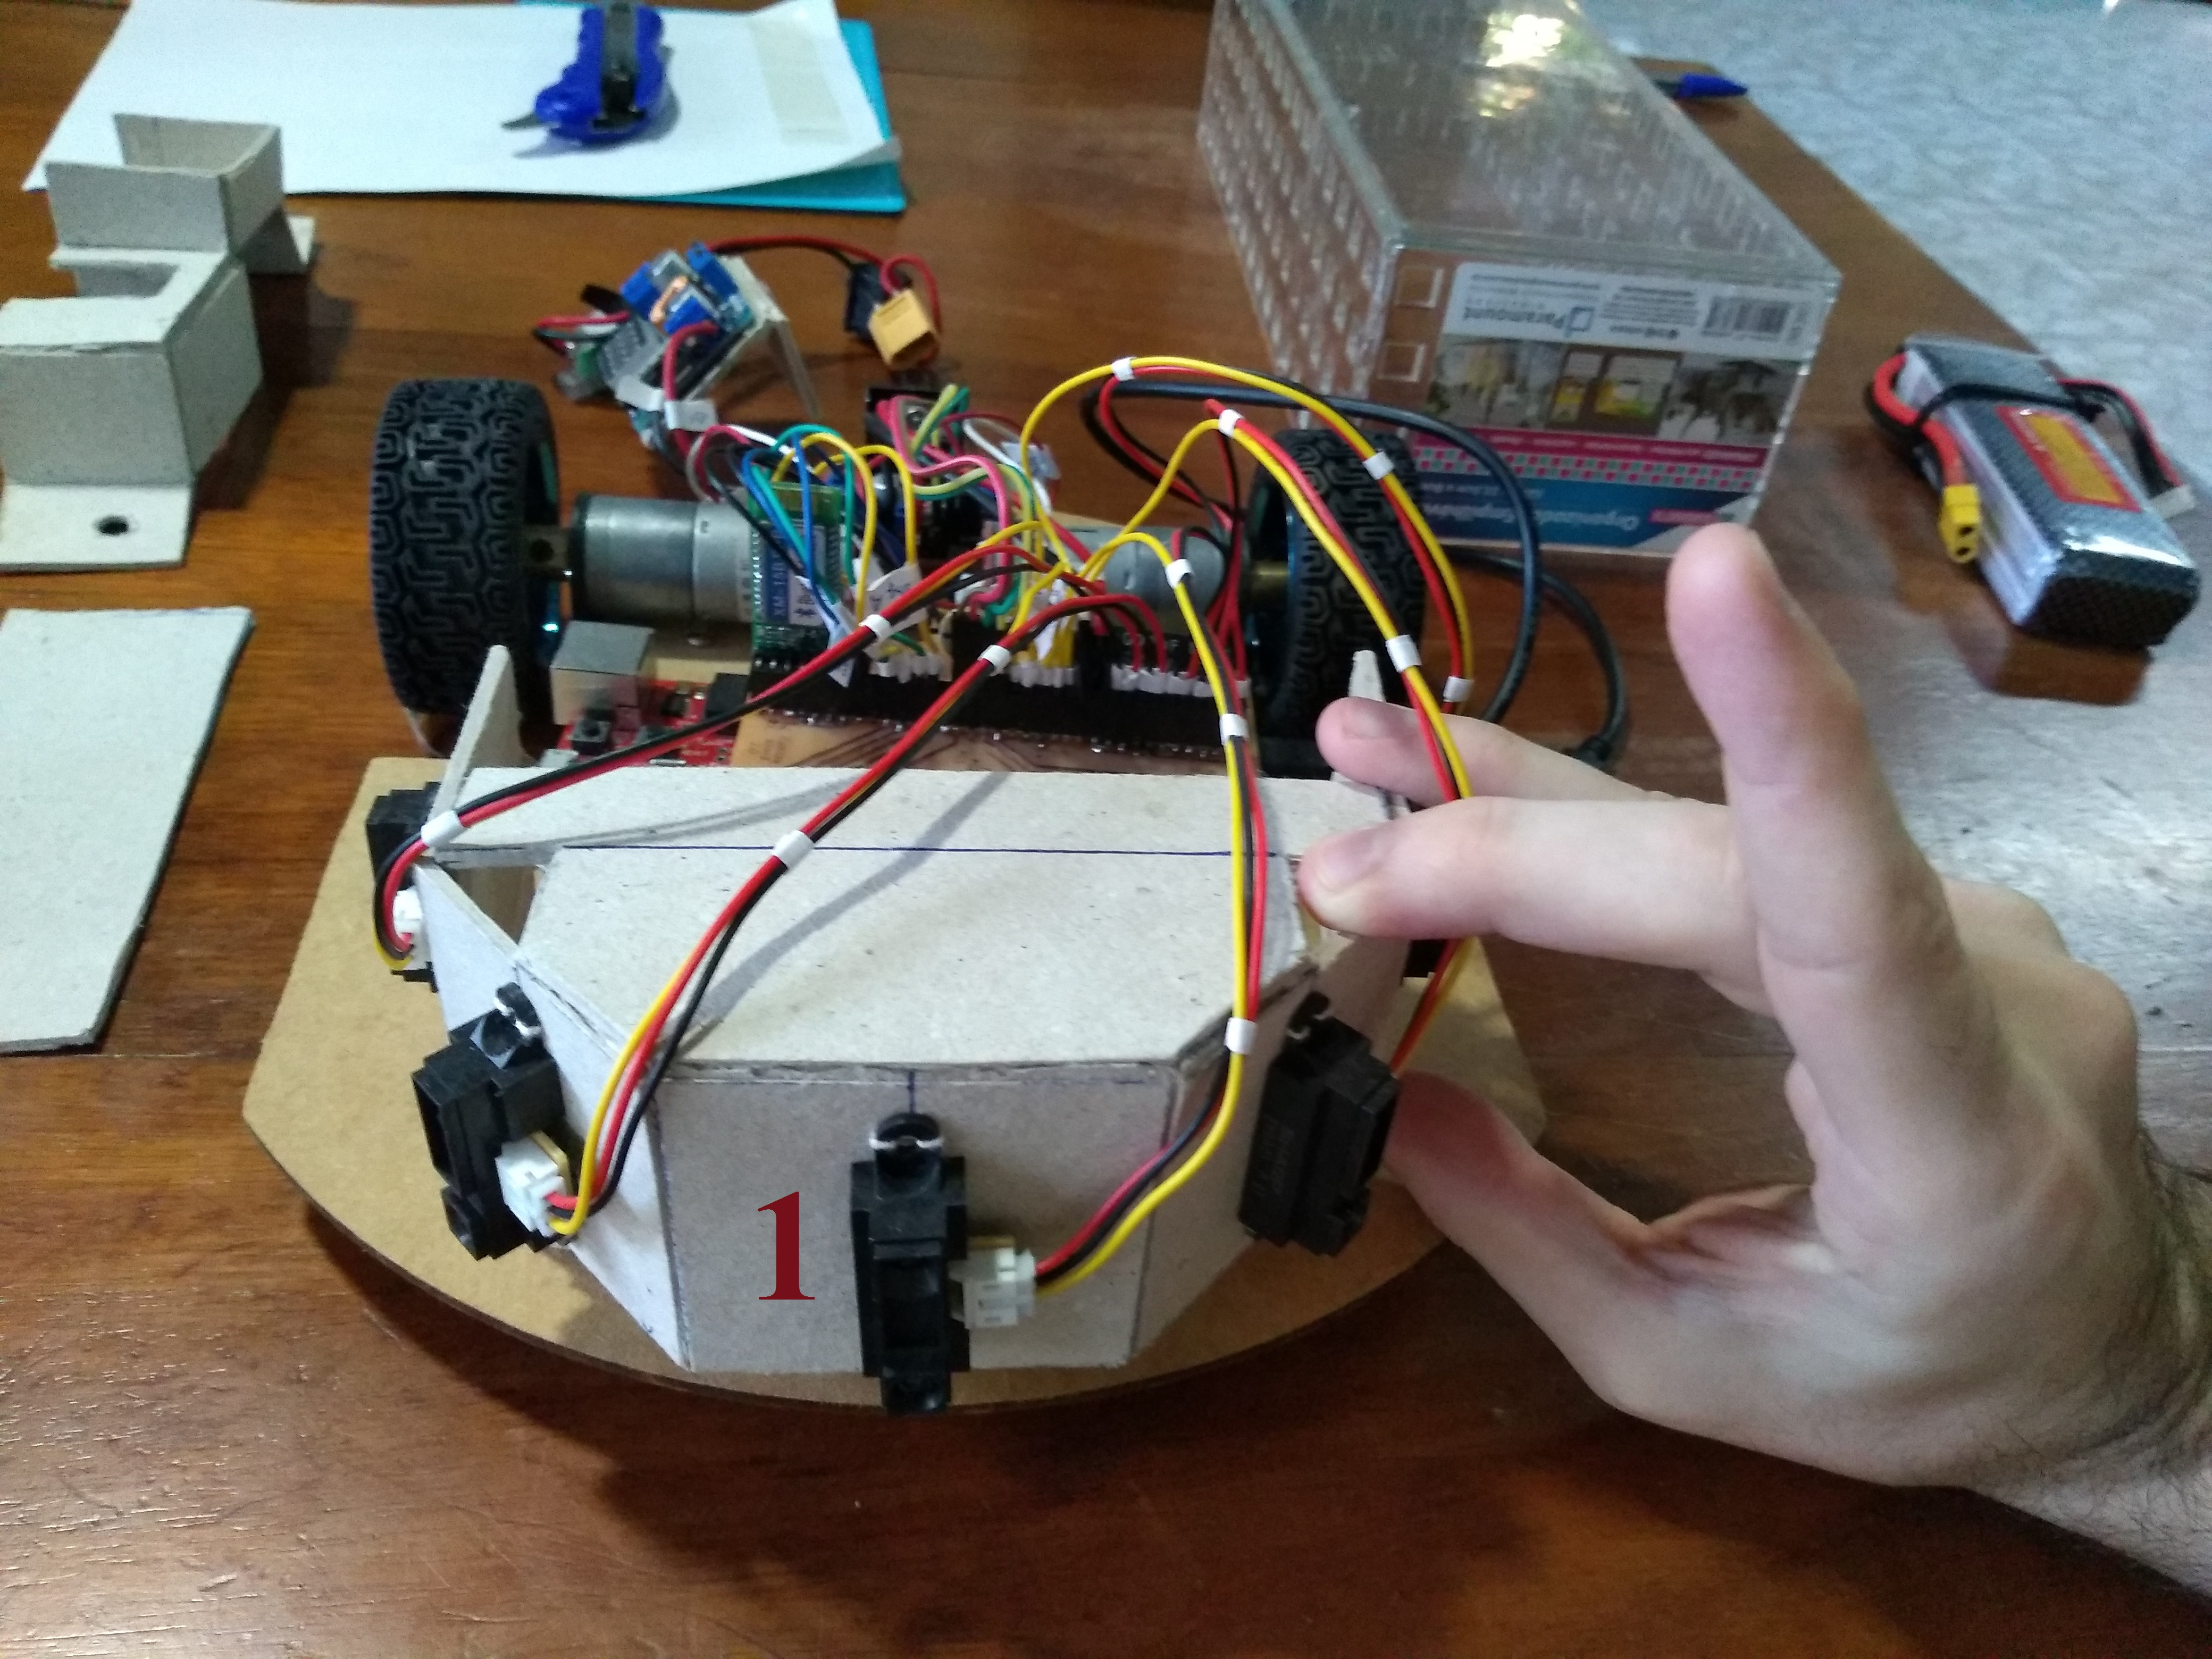
\includegraphics[trim= 0cm 0cm 0cm 0cm,clip,
scale=0.055]{Figuras/RoboMontagem1}
		\subcaption{Posicionamento dos sensores IR}
	  	%\label{fig:test1}
	\end{subfigure}
	~
	\begin{subfigure}[b]{0.49\textwidth}%
		\centering
		% fbox{}
		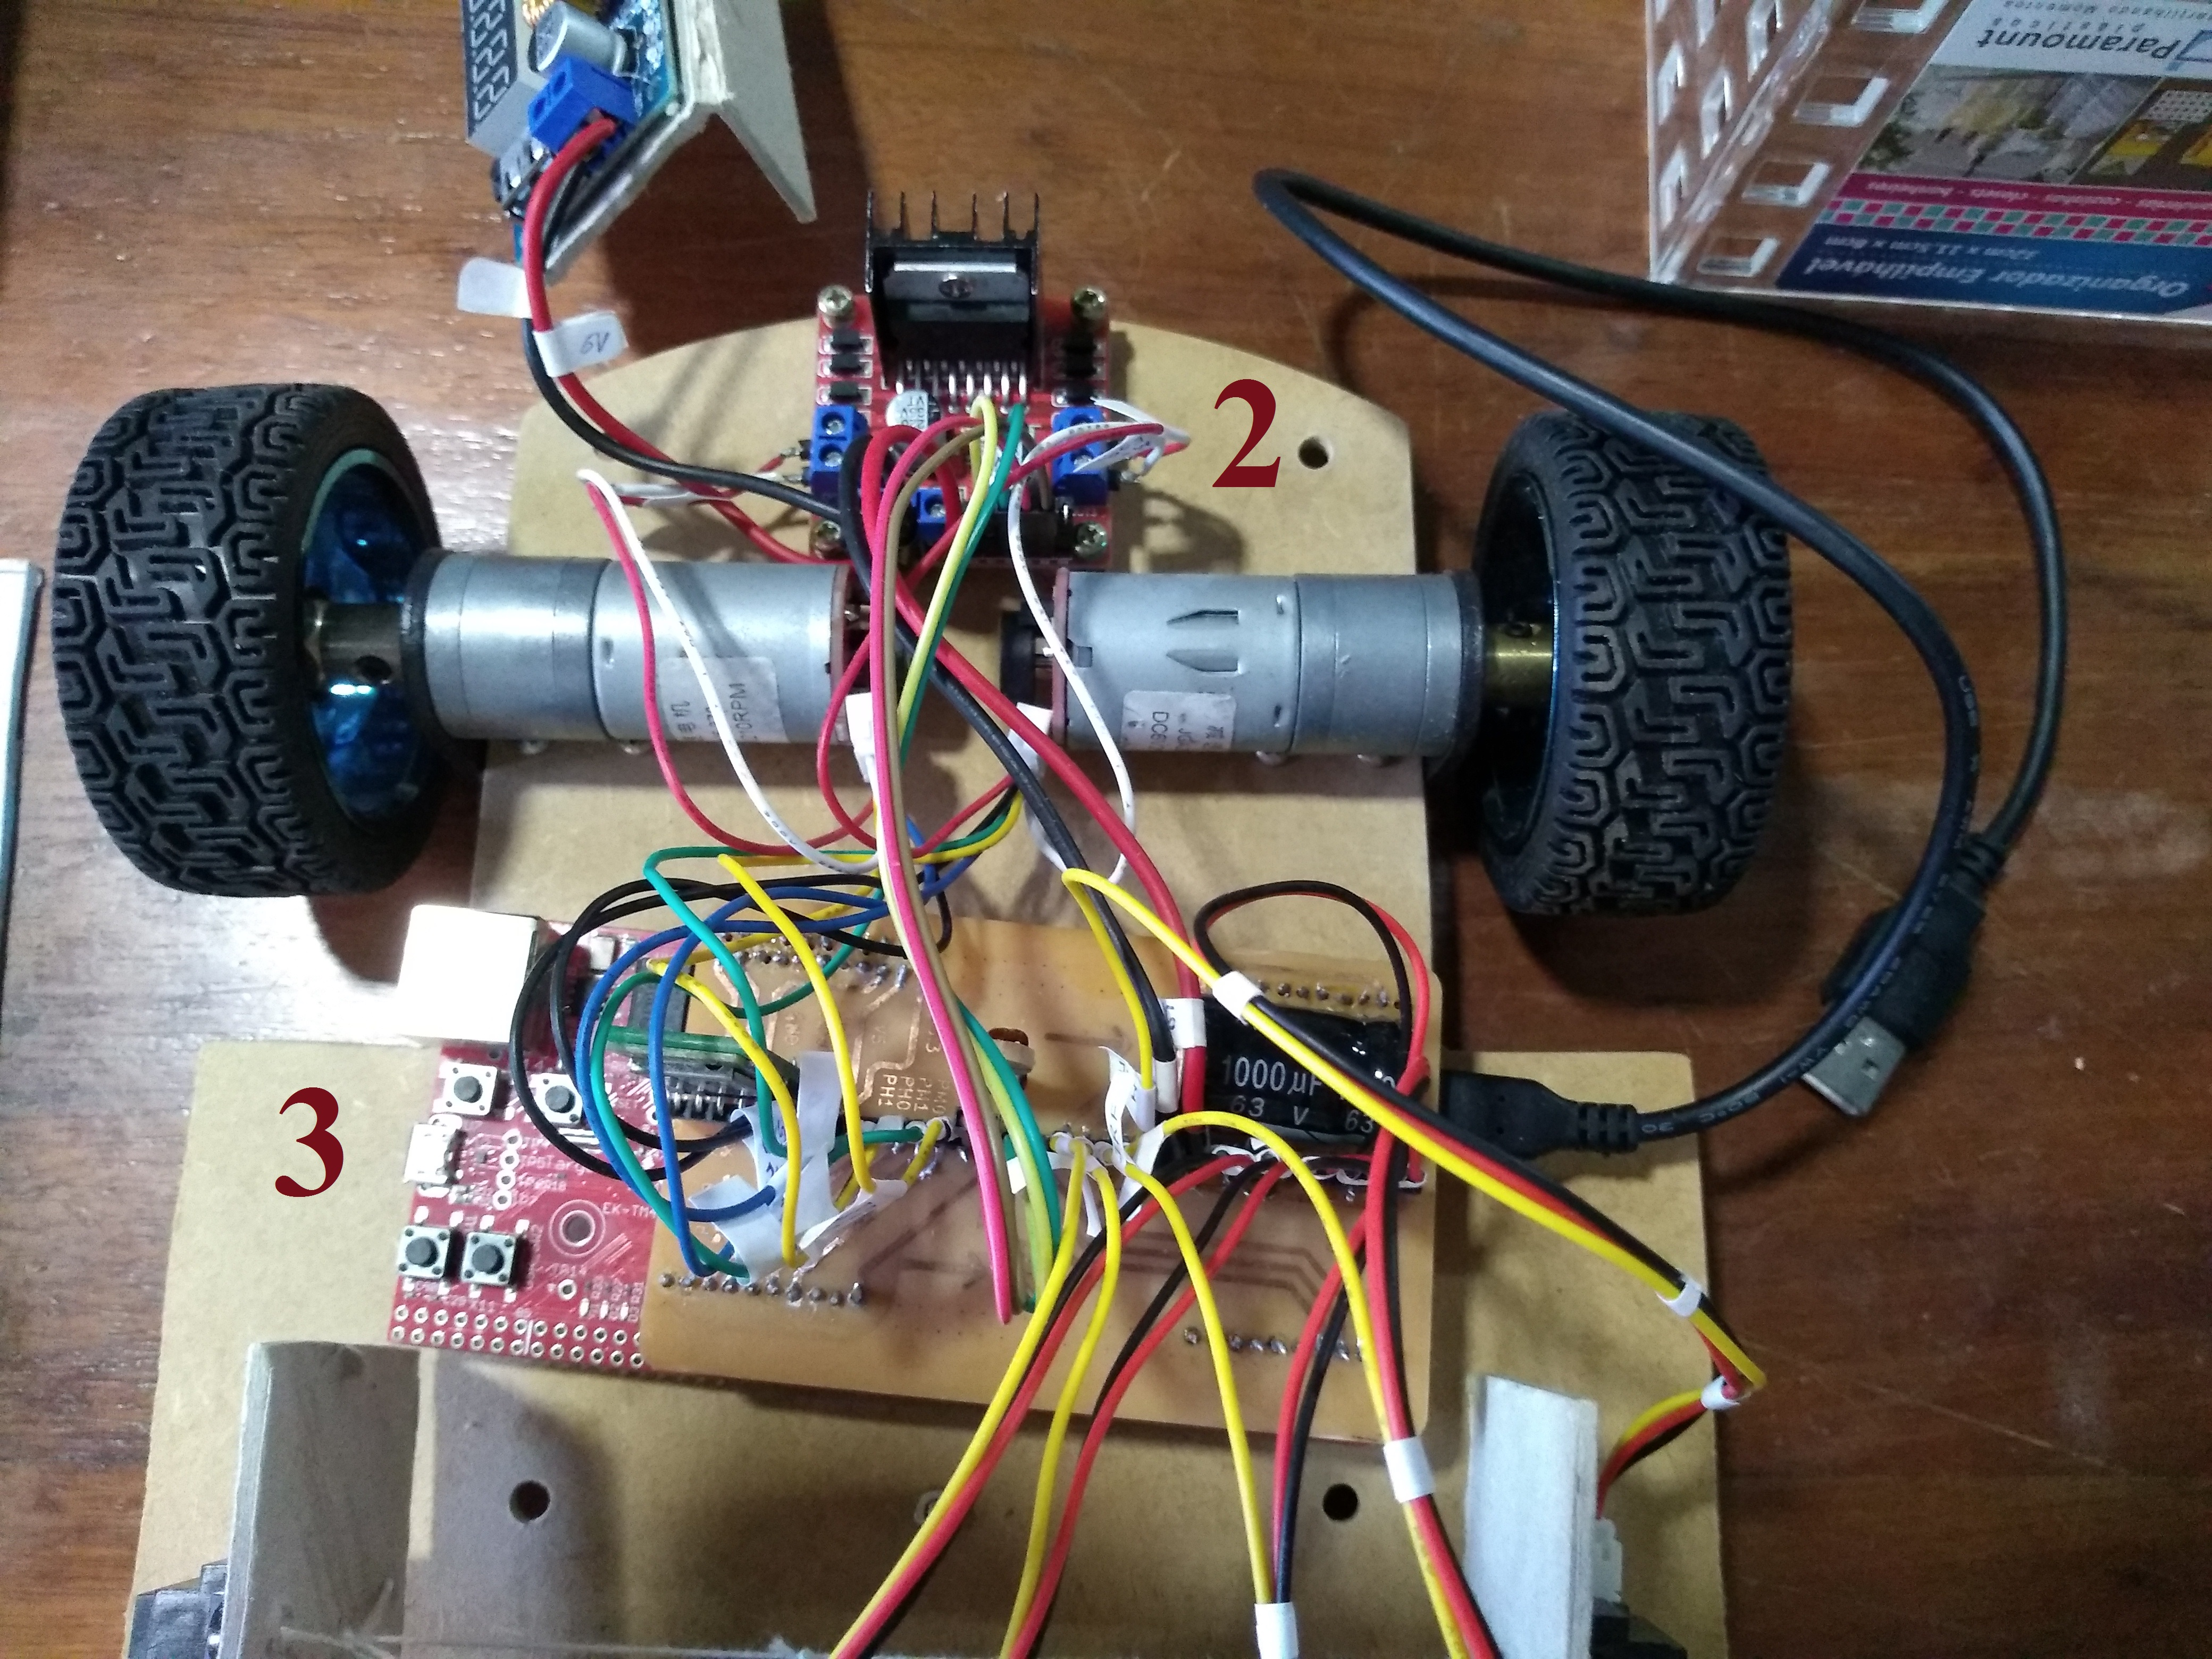
\includegraphics[trim={0cm 0cm 0cm 0cm},clip,
scale=0.055]{Figuras/RoboMontagem2}
		\subcaption{Disposição dos motores e microcontrolador}
	  	%\label{fig:test2}
	\end{subfigure}
	~
	\begin{subfigure}[b]{0.49\textwidth}%
		\centering
		% fbox{}
		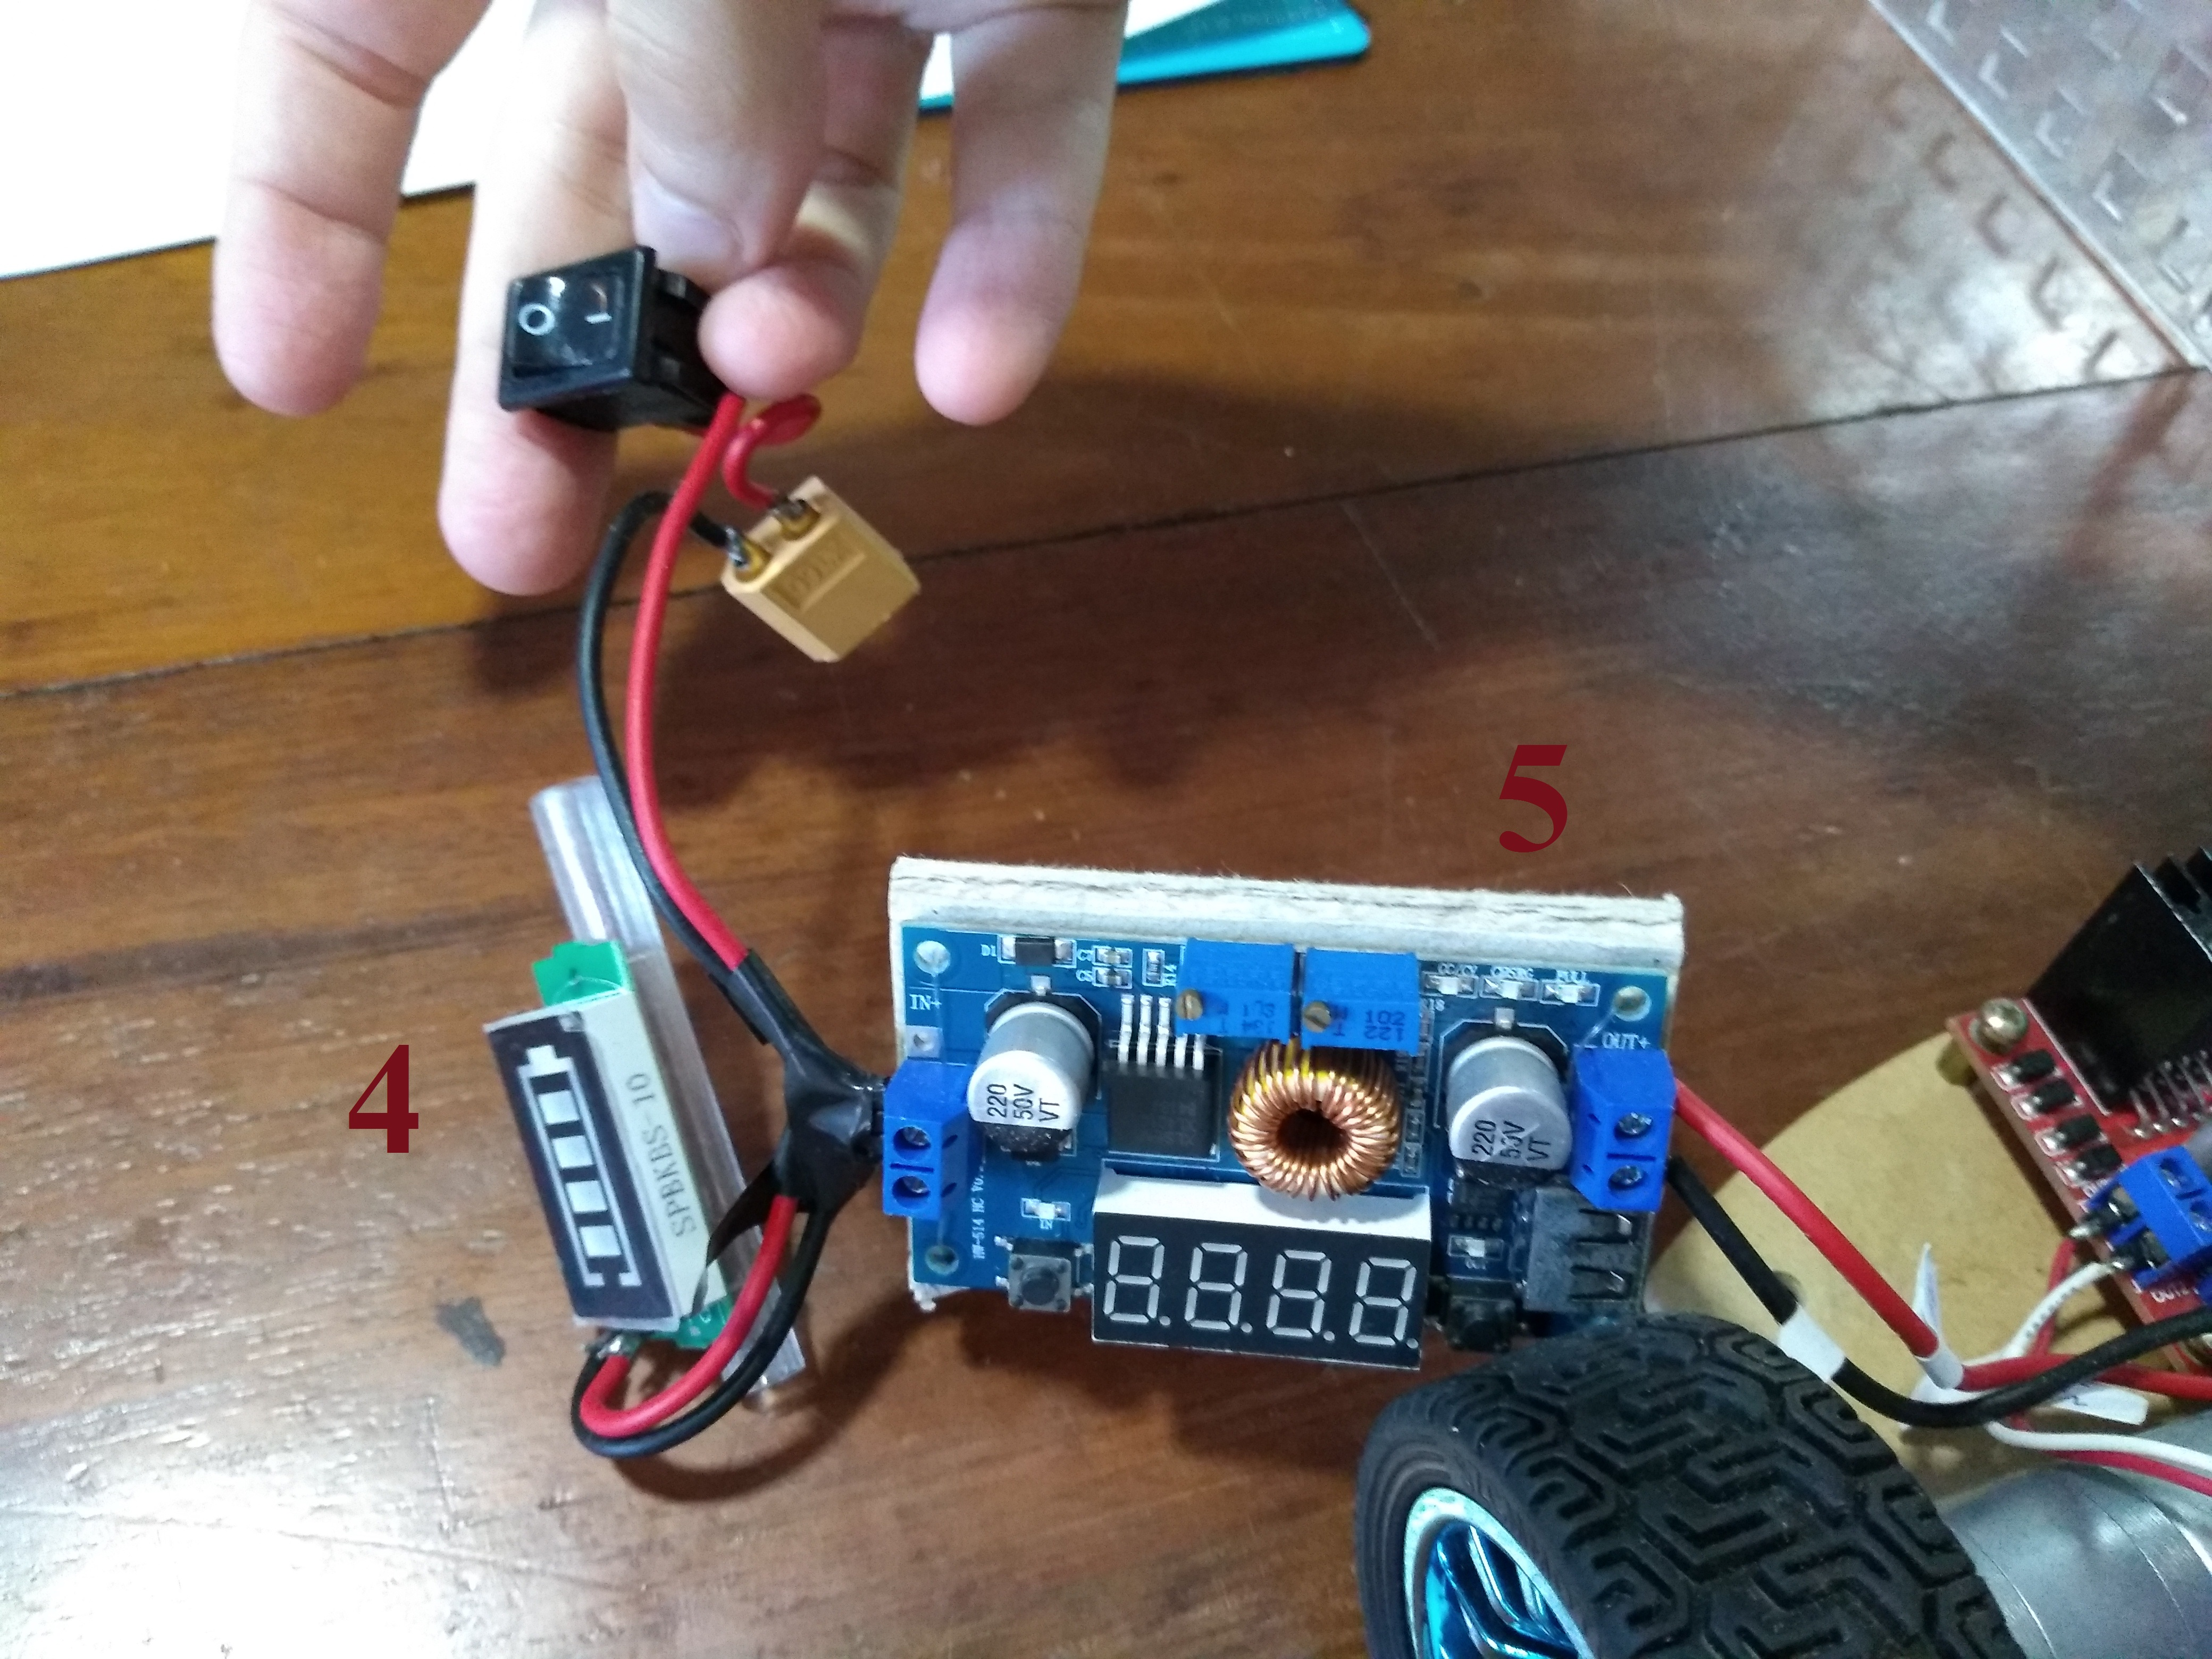
\includegraphics[trim= 0cm 0cm 0cm 0cm,clip,
scale=0.055]{Figuras/RoboMontagem3}
		\subcaption{Regulador de Tensão}
	  	%\label{fig:test1}
	\end{subfigure}
	~
	\begin{subfigure}[b]{0.49\textwidth}%
		\centering
		% fbox{}
		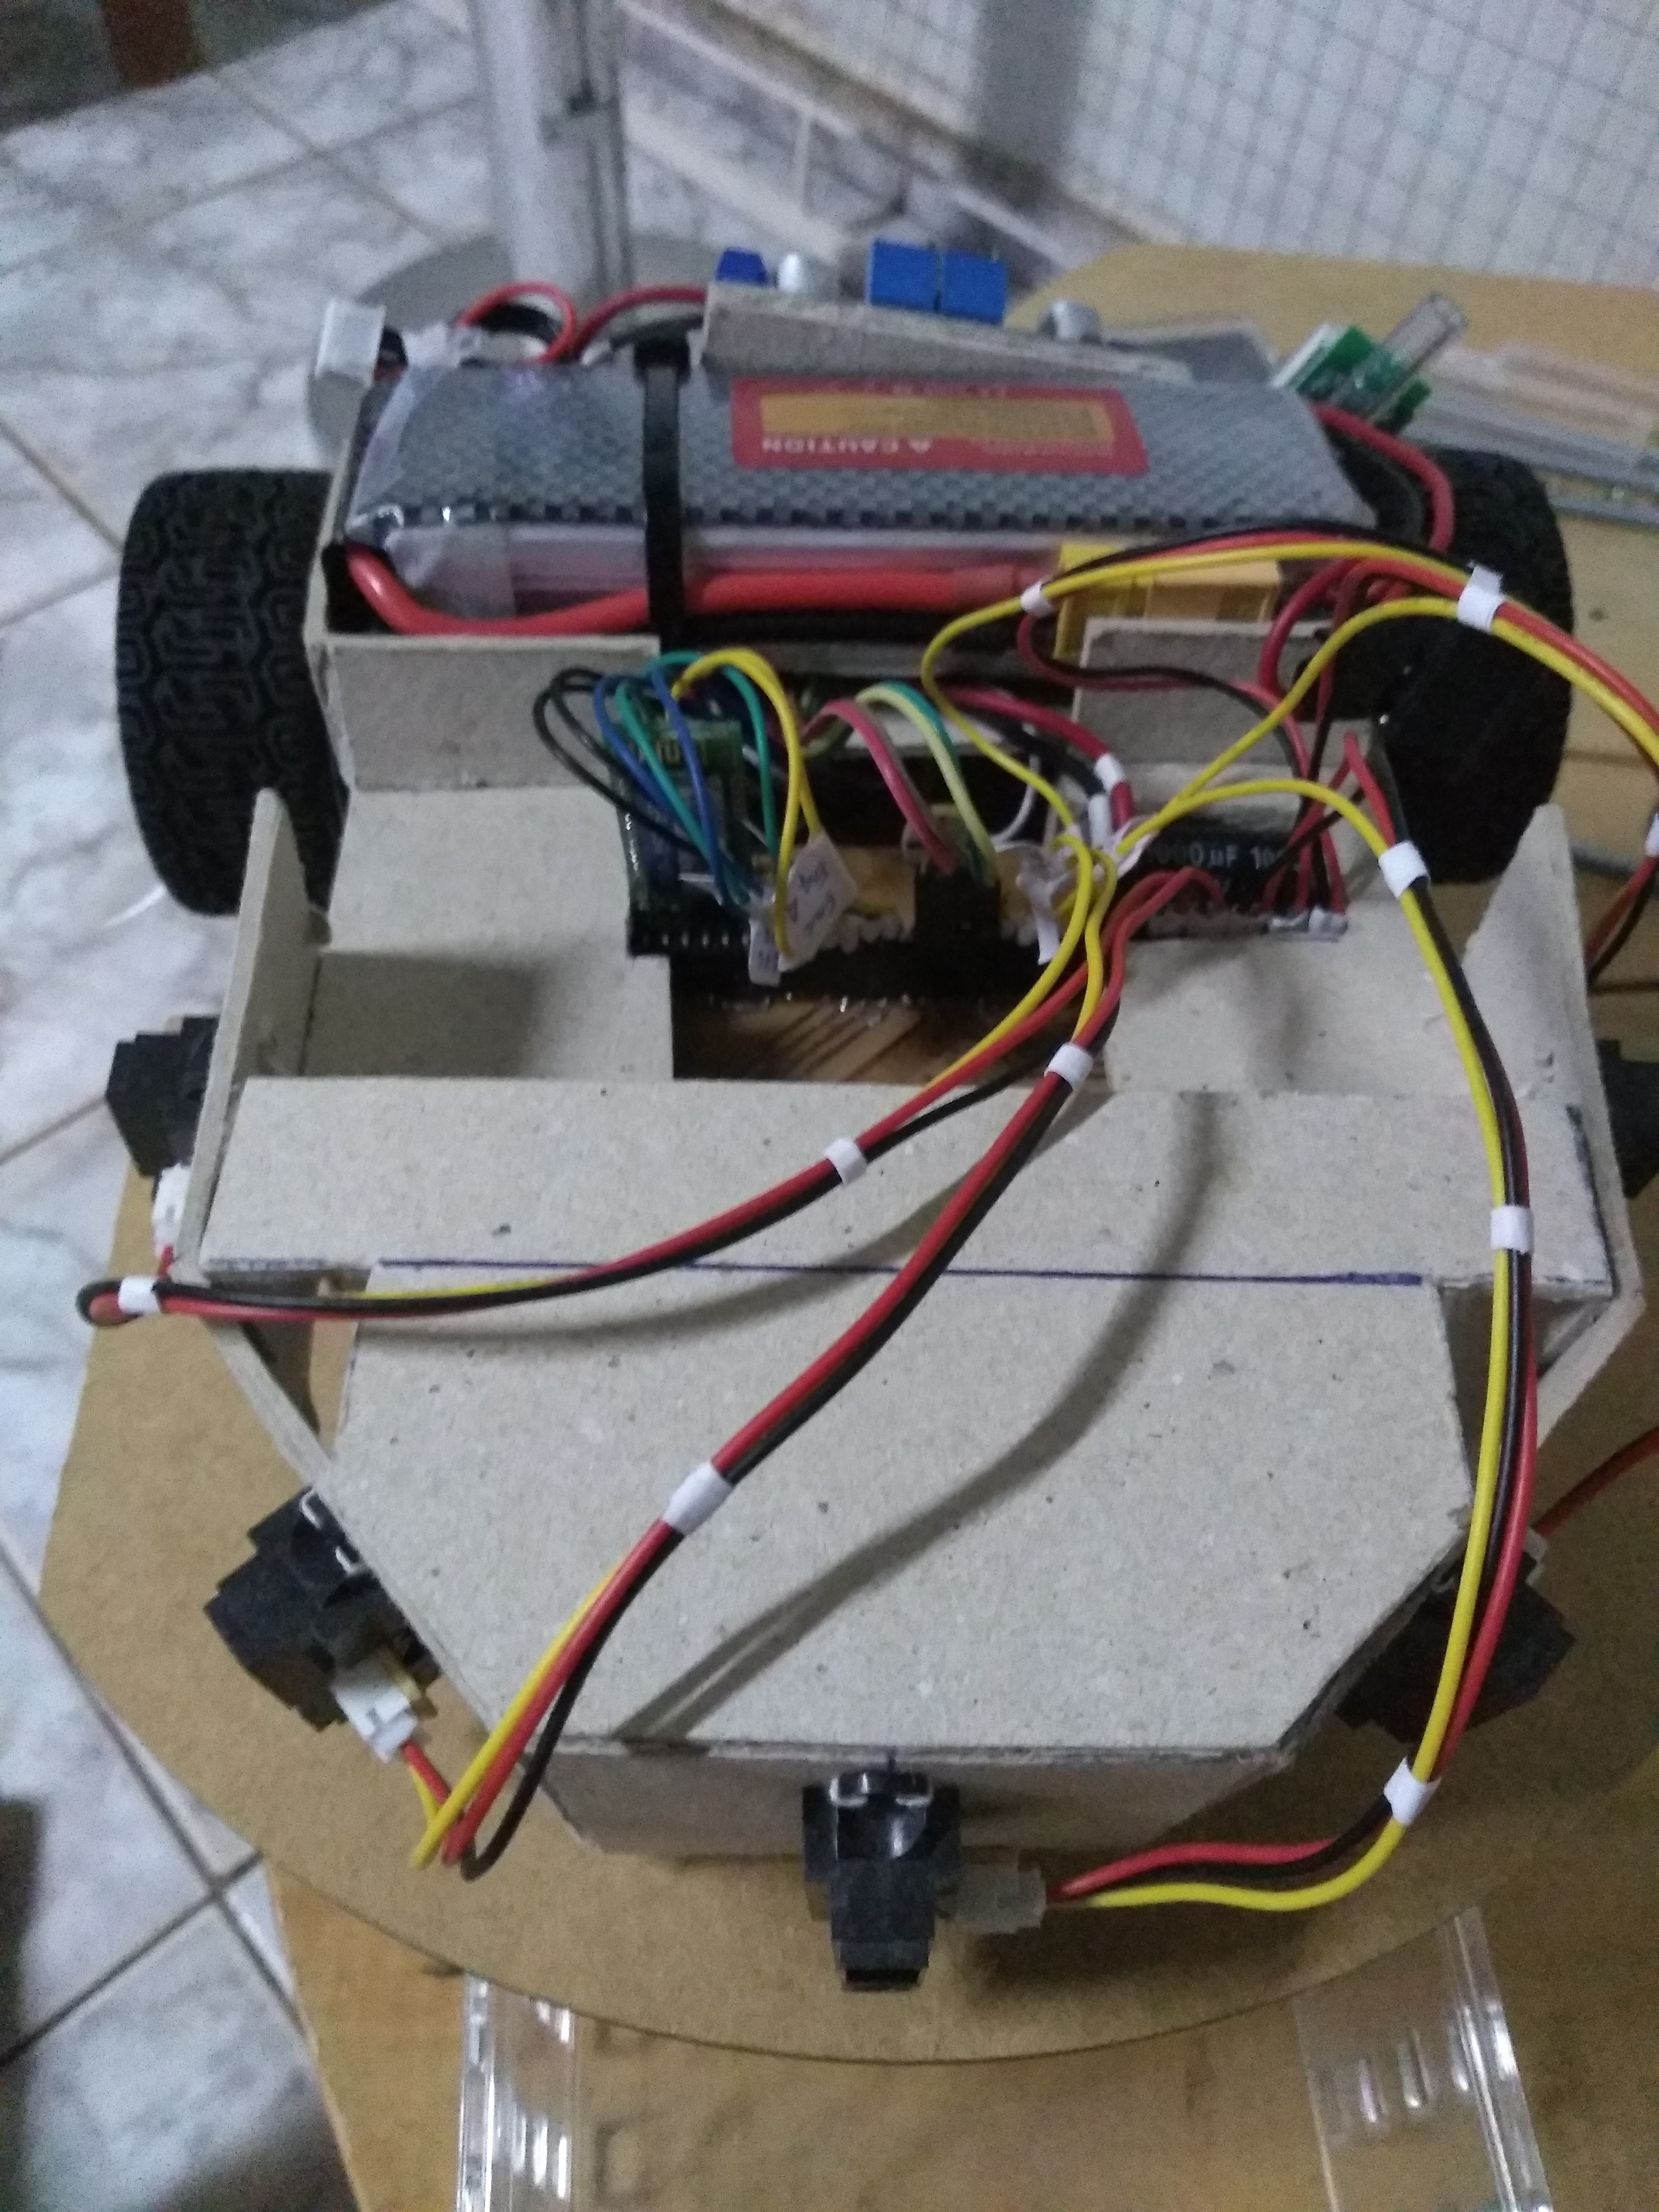
\includegraphics[trim={0cm 0cm 0cm 0cm},clip,
scale=0.055]{Figuras/RoboMontagem4}
		\subcaption{Posicionamento dos componentes}
	  	%\label{fig:test2}
	\end{subfigure}
	
	\textbf{Fonte: autoria própria}
\end{figure}

\subsection{Especificações}

As variáveis L e R na Equação \ref{eq:diff}, para o robô deste trabalho, valem
respectivamente 18 cm e 3,4 cm.

O sensor infravermelho GP2Y0A21YK0F utilizado neste trabalho possui a curva de
tensão por distância representada na Figura \ref{fig:SensorIR}. A faixa de
distância está entre 10 e 80 cm. No QuickBot, é utilizado o sensor GP2Y0A41SK0F,
com distância de medição entre 4 e 30 cm.

\begin{figure}[ht]
	\centering
	\caption{Resposta do sensor infravermelho}
	\label{fig:SensorIR}
	
	%\fbox{}
	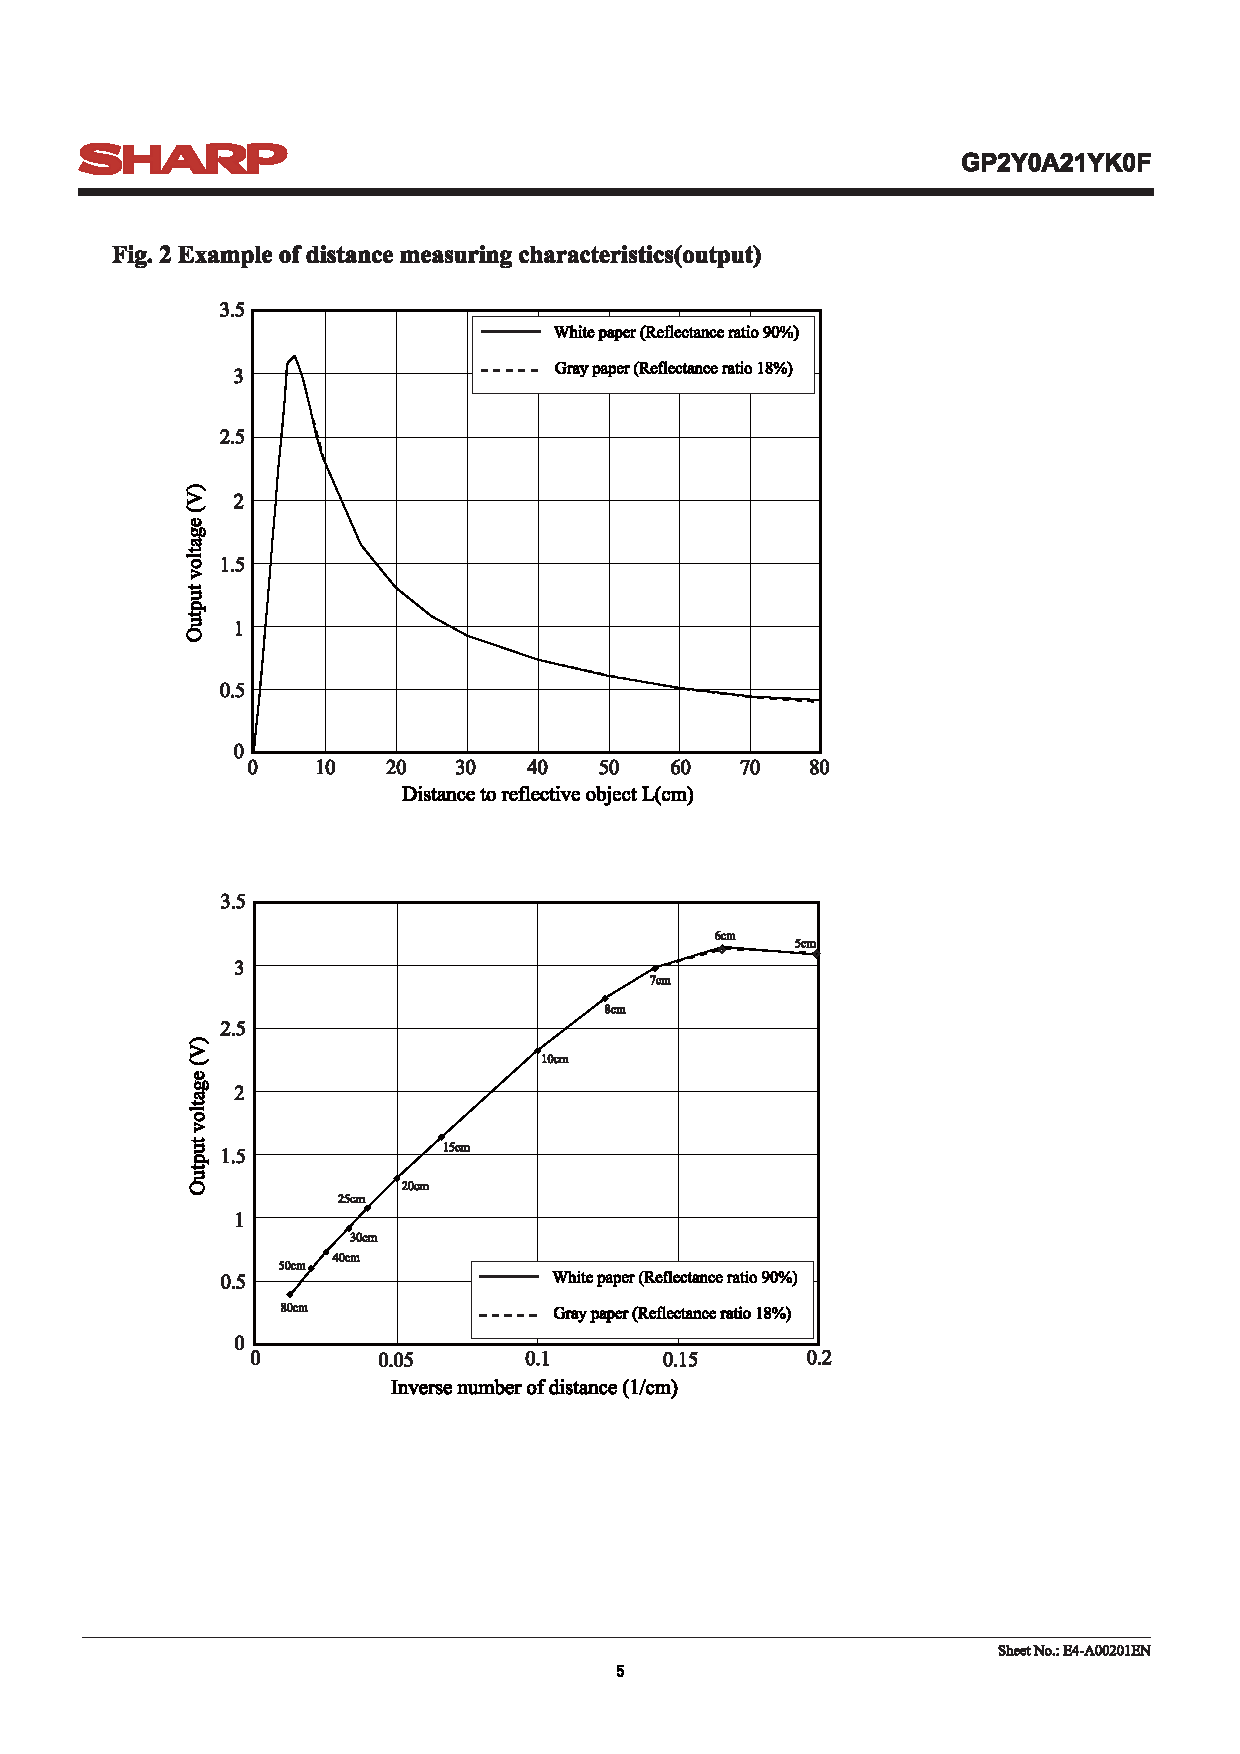
\includegraphics[trim= 3cm 15.8cm 6.5cm 4.8cm,clip,
scale=1]{Figuras/IR_Datasheet_Figure}

	%\begin{tikzpicture}[auto, node distance=2cm, on grid,
%>=latex']%
	
	%\node[anchor=south west,inner sep=0] (image) at (0,0) {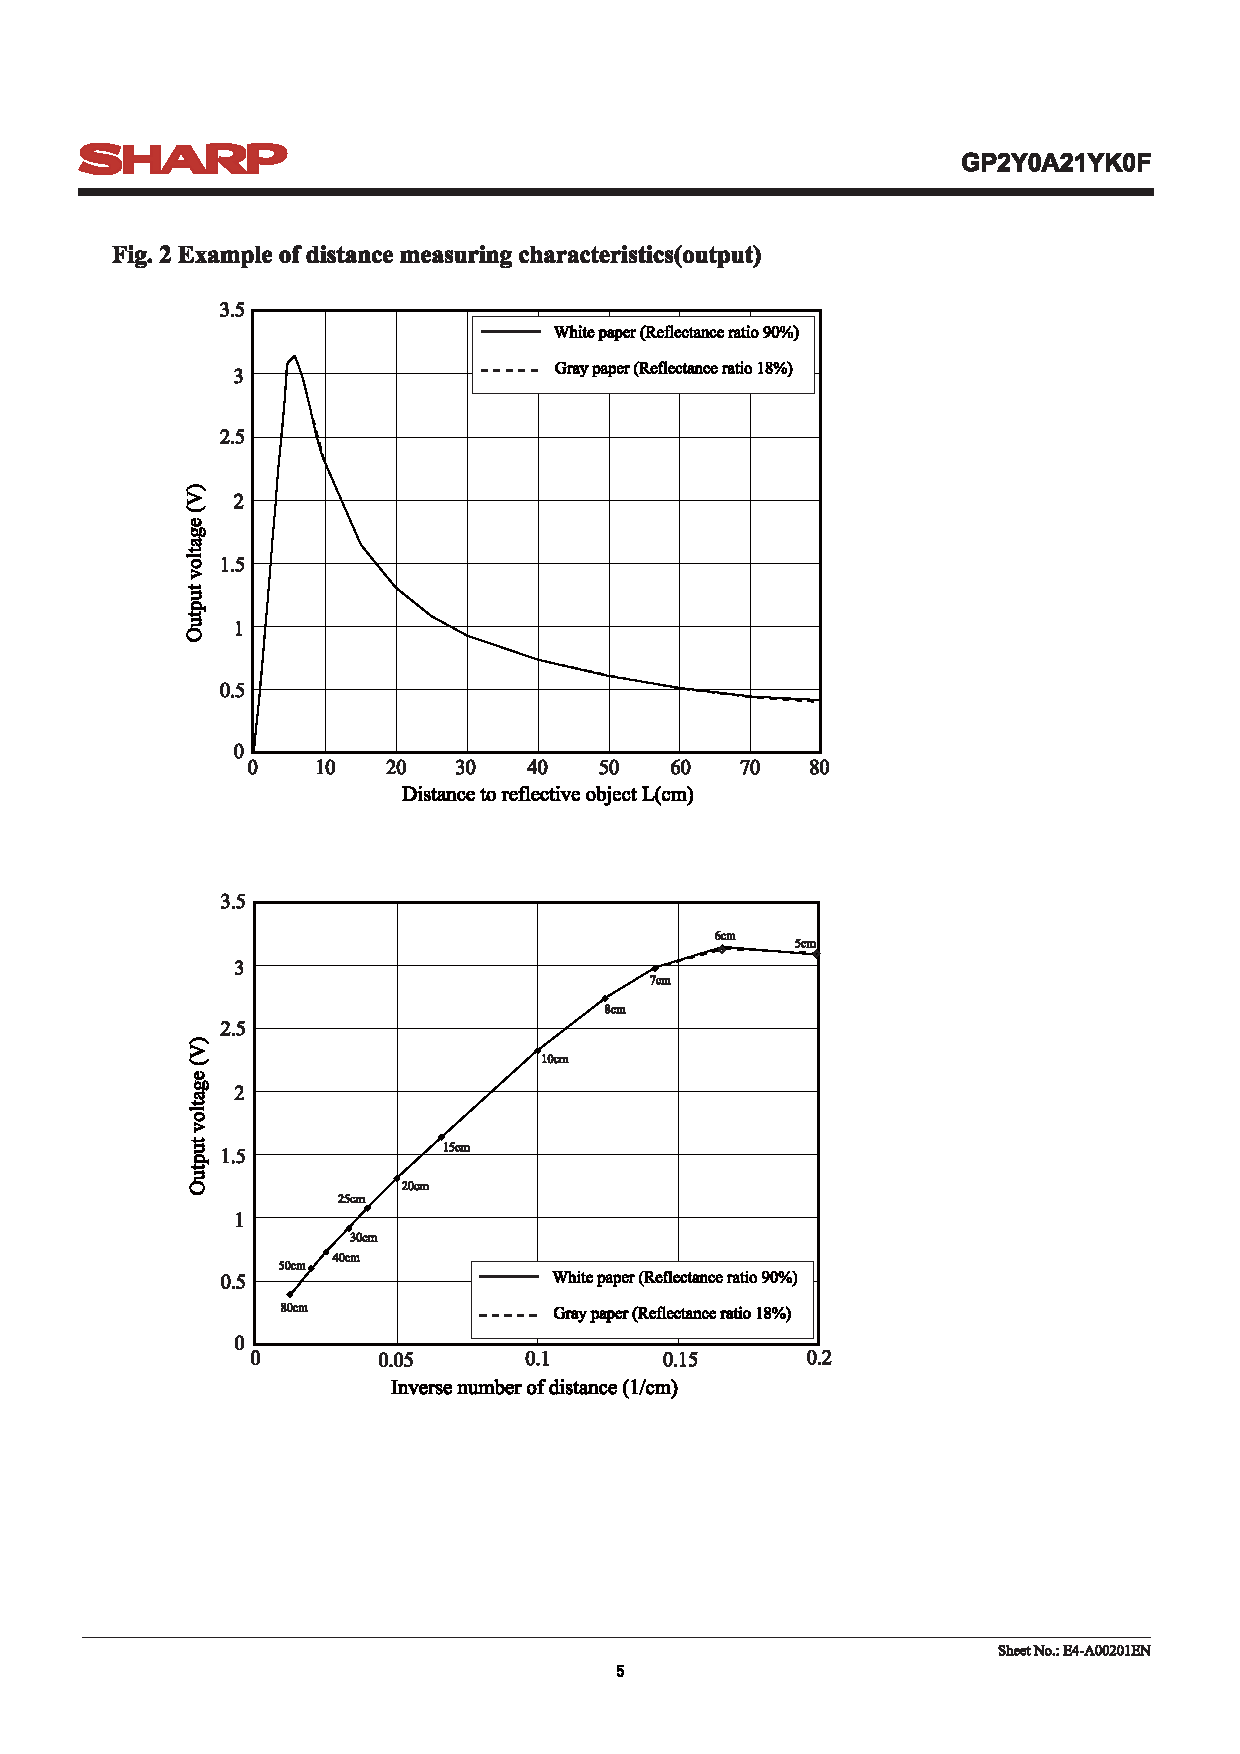
\includegraphics[trim =
%		{3cm 15.8cm 6.5cm 4.8cm}, clip,scale=1]{Figuras/IR_Datasheet_Figure}};
		
%	\node[fill,circle,inner sep=0.1pt, color = red] at (1.29,1.161) {};
%	\node[fill,circle,inner sep=0.1pt, color = red] at (2.525,2.235) {};
	
%	\node[fill,circle,inner sep=0.1pt, color = red] at (1.83,7.75) {};
	
	
%	\node[inner sep = 0 pt, outer sep = 0 pt] (origin) at (1.3,1.15) {};
%	\node[inner sep = 0 pt, outer sep = 0 pt] (teste2) at (2.55,2.25) {};
%	
%	\node[inner sep = 0 pt, outer sep = 0 pt] (P1) at (1.85,7.85) {};
	
	%\draw[-, color = red] (origin) -- (teste2);
	%\draw[-, color = red] (origin) -- (P1);
	
	%\node[] at (0,0) {};
	%\coordinate[] (teste1) {};
	%\coordinate[] (teste2) {};
	
	%\draw[-, color = red] (-18,2) -- (-7,3);
	
%	\end{tikzpicture}


	\textbf{Fonte: \citeonline{datasheet:SensorIR}}
\end{figure}

Para a região da curva onde $d > 5,5 cm$, o polinômio que a aproxima, associando
o inverso da distância pela tensão ($d(v) = \frac{1}{d'(v)}$), obtido utilizando
a função polyfit do Matlab pode ser visto na Equação \ref{eq:PolinomioVx}.
\begin{equation}
	\label{eq:PolinomioVx}
	d'(v) = 21.49298 v^5 + 21.86894 v^4 + 22.25754 v^3 + 22.65912 v^2 + 23.07406 v
	+ 23.50272
\end{equation}

%Odometria

\section{Desenvolvimento dos controladores}

	Nesta seção pretende-se investigar a arquitetura comportamental em robótica 
	móvel para as duas estratégias clássicas de implementação: arbitragem e fusão de 
	comportamentos. Para isso, controladores híbrido e fuzzy serão criados, o primeiro
	para arbitrágem e o segundo para fusão.

	\subsection{Por Controlador Híbrido}
	
	Nesta subseção, pretende-se demonstrar um controlador simples capaz de 
	solucionar o problema de navegação, usando autômato híbrido. Para cada estado
	no autômato, um controlador é selecionado e uma recomendação de saída é 
	calculada. 
	
		\subsubsection{Comportamento ''Ir Para Objetivo''}
		
		\newcommand{\meuRoboLindaoCompIPO}{
	\begin{tikzpicture}[scale = 2]%
		\coordsystwo{I}
		\begin{scope}[shift={(3, 0.9)}]
			\draw[->] (0.3,0) arc (0:30:0.3);
			\draw[-] (0,0) -- (0.4,0);
			\node at (0.5,0.1) {$\phi$};
			
			% Pr 
			\begin{scope}[scale = 0.5]
				\node[color = gray] at (0.1,-0.35) {$P_r$};
			\end{scope}
			\begin{scope}[rotate=30,scale=0.5]
				\begin{scope}[scale=0.9]
					\coordsystwo{R}
				\end{scope}
				\begin{scope}[shift={(0.25,0)},rotate = -90]
					\RoboDiffClean
				\end{scope}
			\end{scope}	
		\end{scope}
		
		% Coord objetivo
		\begin{scope}[shift={(4, 3)}]
			\filldraw (0,0) circle (1pt);
			% Po
			\begin{scope}[scale = 0.5]
				\node[color = gray] at (0.2,-0.45) {$P_o$};
			\end{scope}
		\end{scope}
		
		% retas
		\node[inner sep = 3pt] (P1) at (4,3) {};
		\node[inner sep = 3pt] (P2) at (3,0.9) {};
		
		\draw[->] (0,0) -- (P1);
		\draw[->] (0,0) -- (P2);
		\draw[->] (P2) -- (P1);
		
		% angulo do objetivo
		\draw[->] (0.6,0) arc (0:37:0.6);
		\draw[-] (0,0) -- (0.4,0);
		\node at (0.8,0.4) {$\theta$};
	\end{tikzpicture}%
}%

\newcommand{\RoboDiffClean}{
	% Linhas de baixo, lat esq e dir
	\draw[-, inner sep = 0] (-0.65,-0.75) -- (0.65,-0.75);
	\draw[-, inner sep = 0] (-0.75,-0.65) -- (-0.75,0.5);
	\draw[-, inner sep = 0] (0.75,-0.65) -- (0.75,0.5);
	
	% bordas de baixo
	\draw[-, inner sep = 0] (-0.65,-0.75) -- (-0.75,-0.65);
	\draw[-, inner sep = 0] (0.65,-0.75) -- (0.75,-0.65);
	
	% Retas de cima
	\def\UserL{\fpeval{1.3/(2*cosd(45)+1)}}
	\draw[-, inner sep = 0] (-0.75,0.5) -- (\fpeval{-0.75+\UserL*cosd(45)},
	\fpeval{0.5+\UserL*sind(45)});
	
	\draw[-, inner sep = 0] (0.75,0.5) -- (\fpeval{0.75-\UserL*cosd(45)},
	\fpeval{0.5+\UserL*sind(45)});
	
	\draw[-, inner sep = 0]
	(\fpeval{-0.75+\UserL*cosd(45)},\fpeval{0.5+\UserL*sind(45)}) -- (\fpeval{0.75-\UserL*cosd(45)},
	\fpeval{0.5+\UserL*sind(45)});
	
	% Bola de rolamento
	\filldraw (0,0.45) circle (1.5pt);
	\draw (0,0.45) circle (3pt);
	
	% Desenhar rodas
	\begin{scope}[shift={(-0.75,-0.65)},rotate = 90]
		\draw[rounded corners=2pt] (0,0) rectangle ++(0.8,0.2);
	\end{scope}
	\begin{scope}[shift={(0.75,-0.65)},rotate = 90]
		\draw[rounded corners=2pt] (0,0) rectangle ++(0.8,-0.2);
	\end{scope}	
}

\begin{figure}[ht]
	\centering%
	\caption{Comportamento Ir para Objetivo}%
	\label{fig:CompIPO}%	
	\meuRoboLindaoCompIPO
	
	\textbf{Fonte: autoria própria}
\end{figure}
		
		\subsubsection{Comportamento ''Evitar Obstáculo''}
		
		\newcommand{\meuRoboLindaoCompEO}{

	\begin{scope}[shift={(0,0.3)}]
		% Pr 
		\begin{scope}[shift={(0,-0.3)}, scale = 0.5]
			\node[color = gray] at (0.1,-0.35) {$P_r$};
		\end{scope}
		\begin{scope}[rotate=90,scale=0.5]
			\filldraw (0,0) circle (0.5pt);
			\begin{scope}[shift={(0.25,0)},rotate = -90]
				\RoboDiffClean
			\end{scope}
		\end{scope}
	\end{scope}
		
	% Obstáculo
	\begin{scope}[shift={(2,0)}]
		\obstaculo{3}
	\end{scope}
}%

\newcommand{\obstaculo}[1]{
	\node[inner sep = 0pt] (P1) at (0,0) {};
	\node[inner sep = 0pt] (P2) at (0.5,0) {};
	\node[inner sep = 0pt] (P3) at (0.5,#1) {};
	\node[inner sep = 0pt] (P4) at (0,#1) {};
	\draw (P1) -- (P2);
	\draw (P2) -- (P3);
	\draw (P3) -- (P4);
	\draw (P4) -- (P1);
}

\newcommand{\sensorVisaoTriangular}[1]{
	\draw (0,0) -- (-0.1,#1);
	\draw (0,0) -- (0.1,#1);
	\draw (-0.1,#1) -- (0.1,#1);
}

\newcommand{\sensorVisaoVetor}[1]{
	\draw[->] (0,0) -- (0,#1);
}

\newcommand{\desenharSensoresTriangulo}{
	\node[color = gray] at (-2.58,0.6) {$d_1$};
	\node[color = gray] at (-1.82,2.41) {$d_2$};
	\node[color = gray] at (0,3.07) {$d_3$};
	\node[color = gray] at (1.82,2.41) {$d_4$};
	\node[color = gray] at (2.24,0.6) {$d_5$};
	
	\begin{scope}[shift={(0.38,0.6)},rotate=-90]
		\sensorVisaoTriangular{2-0.38}
	\end{scope}
	\begin{scope}[shift={(-0.38,0.6)},rotate=90]
		\sensorVisaoTriangular{2}
	\end{scope}
	\begin{scope}[shift={(0.28,0.77)},rotate=-45]
		\sensorVisaoTriangular{2}
	\end{scope}
	\begin{scope}[shift={(-0.28,0.77)},rotate=45]
		\sensorVisaoTriangular{2}
	\end{scope}	
	\begin{scope}[shift={(0,0.87)},rotate=0]
		\sensorVisaoTriangular{2}
	\end{scope}
}

\newcommand{\desenharSensoresVetores}{
	\node[color = gray] at (-2.58,0.6) {$v_1$};
	\node[color = gray] at (-1.82,2.41) {$v_2$};
	\node[color = gray] at (0,3.07) {$v_3$};
	\node[color = gray] at (1.82,2.41) {$v_4$};
	\node[color = gray] at (2.24,0.6) {$v_5$};
	
	\begin{scope}[shift={(0.38,0.6)},rotate=-90]
		\sensorVisaoVetor{2-0.38}
	\end{scope}
	\begin{scope}[shift={(-0.38,0.6)},rotate=90]
		\sensorVisaoVetor{2}
	\end{scope}
	\begin{scope}[shift={(0.28,0.77)},rotate=-45]
		\sensorVisaoVetor{2}
	\end{scope}
	\begin{scope}[shift={(-0.28,0.77)},rotate=45]
		\sensorVisaoVetor{2}
	\end{scope}	
	\begin{scope}[shift={(0,0.87)},rotate=0]
		\sensorVisaoVetor{2}
	\end{scope}
}


\begin{figure}[ht]
	\centering%
	\caption{Comportamento Evitar Obstáculo}%
	\label{fig:CompEO}%
	\begin{subfigure}[t]{0.5\textwidth}%
		\centering%
			
		\begin{tikzpicture}[scale = 1.4]%
			\meuRoboLindaoCompEO
			\desenharSensoresTriangulo
		\end{tikzpicture}%
		
		\label{fig:CompEOa}%
		\caption{Sensores infravermelho}%
	\end{subfigure}%
	~
	\begin{subfigure}[t]{0.5\textwidth}%
		\centering%
		
		\begin{tikzpicture}[scale = 1.4]%
			\meuRoboLindaoCompEO
			\desenharSensoresVetores
		\end{tikzpicture}%
			
		\label{fig:CompEOb}%
		\caption{Vetores utilizados}%
	\end{subfigure}%
	\\
	\textbf{Fonte: autoria própria}
\end{figure}
		
		\subsubsection{Comportamento mesclado ''Ir Para Objetivo e Evitar Obstáculo''}
		
		\subsubsection{Mínimos locais}
		
		\newcommand{\meuRoboLindaoCompMinimos}{
	\begin{scope}[shift={(0,0.3)}]
		% Pr 
		\begin{scope}[shift={(0,-0.3)}, scale = 0.5]
			\node[color = gray] at (0.1,-0.35) {$P_r$};
		\end{scope}
		\begin{scope}[rotate=90,scale=0.5]
			\filldraw (0,0) circle (0.5pt);
			\begin{scope}[shift={(0.25,0)},rotate = -90]
				\RoboDiffClean
			\end{scope}
		\end{scope}
	\end{scope}
}%

\newcommand{\obstaculoA}[2]{
	\node[inner sep = 0pt] (P1) at (#1,0) {};
	\node[inner sep = 0pt] (P2) at (\fpeval{#1+(#2/2)},\fpeval{#2*sqrt{2}/2}) {};
	\node[inner sep = 0pt] (P3) at (\fpeval{#1+((3*#2)/2)},\fpeval{#2*sqrt{2}/2}) {};
	\node[inner sep = 0pt] (P4) at (\fpeval{#1+2*#2},0) {};
	\node[inner sep = 0pt] (P5) at (\fpeval{#1+((3*#2)/2)},\fpeval{-(#2*sqrt{2}/2)}) {};
	\node[inner sep = 0pt] (P6) at (\fpeval{#1+(#2/2)},\fpeval{-(#2*sqrt{2}/2)}) {};
	
	\draw[color = darkgray] (P1) -- (P2);
	\draw[color = darkgray] (P2) -- (P3);
	\draw[color = darkgray] (P3) -- (P4);
	\draw[color = darkgray] (P4) -- (P5);
	\draw[color = darkgray] (P5) -- (P6);
	\draw[color = darkgray] (P6) -- (P1);
	
	\node[color = gray] at (#1+#2,-1.3) {Obstáculo 1};
}

\newcommand{\obstaculoB}[3]{
	\node[inner sep = 0pt] (P1) at (#1,#2) {};
	\node[inner sep = 0pt] (P2) at (#1,#2+0.5) {};
	\node[inner sep = 0pt] (P3) at (#1+#3+0.5,#2+0.5) {};
	\node[inner sep = 0pt] (P4) at (#1+#3+0.5,-#2-0.5) {};
	
	\node[inner sep = 0pt] (P5) at (#1,-#2-0.5) {};
	\node[inner sep = 0pt] (P6) at (#1,-#2) {};
	\node[inner sep = 0pt] (P7) at (#1+#3,-#2) {};
	\node[inner sep = 0pt] (P8) at (#1+#3,#2) {};
	
	\draw[color = darkgray] (P1) -- (P2);
	\draw[color = darkgray] (P2) -- (P3);
	\draw[color = darkgray] (P3) -- (P4);
	\draw[color = darkgray] (P4) -- (P5);
	\draw[color = darkgray] (P5) -- (P6);
	\draw[color = darkgray] (P6) -- (P7);
	\draw[color = darkgray] (P7) -- (P8);
	\draw[color = darkgray] (P8) -- (P1);
	
	\node[color = gray] at (#1+0.25+#3/2,-2.8) {Obstáculo 2};
}

\newcommand{\obstaculoC}[2]{
	\node[inner sep = 0pt] (P1) at (#1,#2+0.5) {};
	\node[inner sep = 0pt] (P2) at (#1+0.5,#2+0.5) {};
	\node[inner sep = 0pt] (P3) at (#1+0.5,-#2-0.5) {};
	\node[inner sep = 0pt] (P4) at (#1,-#2-0.5) {};
	
	\draw[color = darkgray] (P1) -- (P2);
	\draw[color = darkgray] (P2) -- (P3);
	\draw[color = darkgray] (P3) -- (P4);
	\draw[color = darkgray] (P4) -- (P1);
	
	\node[color = gray] at (#1+0.25,-2.8) {Obstáculo 3};
}

\begin{figure}[ht]
	\centering%
	\caption{Tipos de obstáculos}%
	\label{fig:CompSP}%
		
	\begin{tikzpicture}[scale = 1.4]%
		% Robô
		\begin{scope}[rotate=-90]
			\meuRoboLindaoCompMinimos
		\end{scope}
		\obstaculoA{2}{1.5}
		\obstaculoB{4}{2}{2}
		\obstaculoC{8}{2}
		
		\begin{scope}[shift={(10,0)}]
			\filldraw (0,0) circle (1.5pt);
			\node[color = gray] at (0,-0.35) {Objetivo};
		\end{scope}
	\end{tikzpicture}%

	\textbf{Fonte: autoria própria}
\end{figure}
		
		\subsubsection{Comportamento ''Seguir parede''}
		
		\newcommand{\meuRoboLindaoCompSP}{
	\begin{scope}[shift={(0,0.3)}]
		% Pr 
		\begin{scope}[shift={(0,-0.3)}, scale = 0.5]
			\node[color = gray] at (0.1,-0.35) {$P_r$};
		\end{scope}
		\begin{scope}[rotate=90,scale=0.5]
			\filldraw (0,0) circle (0.5pt);
			\begin{scope}[shift={(0.25,0)},rotate = -90]
				\RoboDiffClean
			\end{scope}
		\end{scope}
	\end{scope}
}%

\newcommand{\parede}[2]{
	\node[inner sep = 0pt] (P1) at (0,0) {};
	\node[inner sep = 0pt] (P2) at (#2,0) {};
	\node[inner sep = 0pt] (P3) at (#2,0.5) {};
	\node[inner sep = 0pt] (P4) at (0.5,0.5) {};
	\node[inner sep = 0pt] (P5) at (0.5,#1) {};
	\node[inner sep = 0pt] (P6) at (0,#1) {};
	\draw[color = darkgray] (P1) -- (P2);
	\draw[color = darkgray] (P2) -- (P3);
	\draw[color = darkgray] (P3) -- (P4);
	\draw[color = darkgray] (P4) -- (P5);
	\draw[color = darkgray] (P5) -- (P6);
	\draw[color = darkgray] (P6) -- (P1);
}

\newcommand{\sensorVisaoTriangularSp}[1]{
	\draw[color = gray] (0,0) -- (-0.1,#1);
	\draw[color = gray] (0,0) -- (0.1,#1);
	\draw[color = gray] (-0.1,#1) -- (0.1,#1);
}

\newcommand{\sensorVisaoVetorSp}[1]{
	\draw[->] (0,0) -- (0,#1);
}

\newcommand{\desenharSensoresTrianguloSPa}{
	\begin{scope}[shift={(0.38,0.6)},rotate=-90]
		\sensorVisaoTriangularSp{2}
	\end{scope}
	\begin{scope}[shift={(-0.38,0.6)},rotate=90]
		\sensorVisaoTriangularSp{2-1.3}
	\end{scope}
	\begin{scope}[shift={(0.28,0.77)},rotate=-45]
		\sensorVisaoTriangularSp{2}
	\end{scope}
	\begin{scope}[shift={(-0.28,0.77)},rotate=45]
		\sensorVisaoTriangularSp{2}
	\end{scope}	
	\begin{scope}[shift={(0,0.87)},rotate=0]
		\sensorVisaoTriangularSp{2}
	\end{scope}
}

\newcommand{\desenharSensoresTrianguloSPb}{
	\begin{scope}[shift={(0.38,0.6)},rotate=-90]
		\sensorVisaoTriangularSp{2-0.9}
	\end{scope}
	\begin{scope}[shift={(-0.38,0.6)},rotate=90]
		\sensorVisaoTriangularSp{2}
	\end{scope}
	\begin{scope}[shift={(0.28,0.77)},rotate=-45]
		\sensorVisaoTriangularSp{2-0.5}
	\end{scope}
	\begin{scope}[shift={(-0.28,0.77)},rotate=45]
		\sensorVisaoTriangularSp{2}
	\end{scope}	
	\begin{scope}[shift={(0,0.87)},rotate=0]
		\sensorVisaoTriangularSp{2-1}
	\end{scope}
}

\newcommand{\desenharLinhasParedeA}{
	\begin{scope}[shift={(-0.38,0.6)},rotate=90]
		\begin{scope}[shift={(0,2-1.3)}]
			\node[inner sep = 0pt] (P1) at (0,0) {};
		\end{scope}
	\end{scope}
	\begin{scope}[shift={(-0.28,0.77)},rotate=45]
		\begin{scope}[shift={(0,2)}]
			\node[inner sep = 0pt] (P2) at (0,0) {};
		\end{scope}
	\end{scope}
	
	\draw (P1) -- (P2);
}

\newcommand{\desenharLinhasParedeB}{
	\begin{scope}[shift={(0.38,0.6)},rotate=-90]
		\begin{scope}[shift={(0,2-0.9)}]
			\node[inner sep = 0pt] (P1) at (0,0) {};
		\end{scope}
	\end{scope}
	\begin{scope}[shift={(0,0.87)},rotate=0]
		\begin{scope}[shift={(0,2-1)}]
			\node[inner sep = 0pt] (P2) at (0,0) {};
		\end{scope}
	\end{scope}
	
	\draw (P1) -- (P2);
}

\begin{figure}[ht]
	\centering%
	\caption{Comportamento Seguir Parede}%
	\label{fig:CompSP}%
	\begin{subfigure}[t]{0.5\textwidth}%
		\centering%
		\begin{tikzpicture}[scale = 1.4]%
			% Obstáculo
			\parede{3}{2}
			% Robô
			\begin{scope}[shift={(-1.1,1.4)},rotate=180]
				\meuRoboLindaoCompSP
				\desenharSensoresTrianguloSPa
				\desenharLinhasParedeA
			\end{scope}
		\end{tikzpicture}%
		
		\label{fig:CompSPa}%
		\caption{Parede subestimada}%
	\end{subfigure}%
	~
	\begin{subfigure}[t]{0.5\textwidth}%
		\centering%
		\begin{tikzpicture}[scale = 1.4]%
			% Obstáculo
			\begin{scope}[shift={(0,0)},xscale=-1,yscale=1]
				\parede{3}{4}
			\end{scope}
			% Robô
			\begin{scope}[shift={(-2.4,2)},rotate=-90]
				\meuRoboLindaoCompSP
				\desenharSensoresTrianguloSPb
				\desenharLinhasParedeB
			\end{scope}
		\end{tikzpicture}%
			
		\label{fig:CompSPb}%
		\caption{Parede superestimada}%
	\end{subfigure}%
	\\
	\textbf{Fonte: autoria própria}
\end{figure}
		
		\newcommand{\desenharLinhasParedeC}[2]{
	\begin{scope}[shift={(-0.38,0.6)},rotate=90]
		\begin{scope}[shift={(0,2-1.3)}]
			\node[inner sep = 0pt] (P1) at (0,0) {};
		\end{scope}
	\end{scope}
	\begin{scope}[shift={(-0.28,0.77)},rotate=45]
		\begin{scope}[shift={(0,2)}]
			\node[inner sep = 0pt] (P2) at (0,0) {};
		\end{scope}
	\end{scope}
	
	\draw (P1) -- (P2);
	
	% linhas continuacao:
	\def\UserVetAX{-1.08}
	\def\UserVetAY{0.6}
	
	\def\UserVetXNum{\fpeval{-0.28-sqrt(2)+1.08}}
	\def\UserVetYNum{\fpeval{0.77+sqrt(2)-0.6}}
	\def\UserVetMod{\fpeval{sqrt(\UserVetXNum*\UserVetXNum + \UserVetYNum*\UserVetYNum)}}
	
	\def\UserVetX{\fpeval{\UserVetXNum/\UserVetMod}}
	\def\UserVetY{\fpeval{\UserVetYNum/\UserVetMod}}
	
	\def\UserLinhaTrasX{\fpeval{-1.08 -\UserVetX*#1}}
	\def\UserLinhaTrasY{\fpeval{0.6 -\UserVetY*#1}}
	\def\UserLinhaFrenteX{\fpeval{-0.28-sqrt(2) +\UserVetX*#2}}
	\def\UserLinhaFrenteY{\fpeval{0.77+sqrt(2) +\UserVetY*#2}}
			
	\draw [dashed] (P1) -- (\UserLinhaTrasX,\UserLinhaTrasY);
	\draw [dashed] (P2) -- (\UserLinhaFrenteX,\UserLinhaFrenteY);
	
	\def\distance{\fpeval{\UserVetX * \UserVetAX + \UserVetY * (\UserVetAY - 0.3)}}
	\begin{scope}[shift={(0,0.3)}]
		\def\UserVetPerpX{\fpeval{\UserVetAX-\distance*\UserVetX}}
		\def\UserVetPerpY{\fpeval{(\UserVetAY - 0.3)-\distance*\UserVetY}}
		\def\UserVetPerpNormX{\UserVetPerpX/(sqrt(\UserVetPerpX*\UserVetPerpX + \UserVetPerpY*\UserVetPerpY))}
		\def\UserVetPerpNormY{\UserVetPerpY/(sqrt(\UserVetPerpX*\UserVetPerpX + \UserVetPerpY*\UserVetPerpY))}
	
		\draw[-{Latex[length=2mm]}] (0,0) -- (P1) node [black,midway,yshift=-0.21cm,xshift=0.1cm] {$u_a$};
		\begin{scope}[shift={(P1)}]
			\draw[-{Latex[length=2mm]}] (0,0) -- (\UserVetX, \UserVetY) node [black,midway,xshift=-0.3cm,yshift=0.1cm] {$u_t$};
		\end{scope}
		\draw[-{Latex[length=2mm]}] (0,0) -- (\UserVetPerpX, \UserVetPerpY)
		node [black,midway,yshift=0.3cm,xshift=0.2] {$u_p$};

		\def\UserChavesX{\fpeval{\UserVetAX-\distance*\UserVetX}}
		\def\UserChavesY{\fpeval{(\UserVetAY - 0.3)-\distance*\UserVetY}}	
		\draw [decorate,decoration={brace,amplitude=10pt},xshift=-2pt,yshift=-2pt]
			(\UserChavesX, \UserChavesY) -- (\fpeval{-1.08},\fpeval{0.3}) 
			node [black,midway,xshift=0.6cm, yshift=0.1cm] {$d$};
			
		% angulo reto:
		\def\UserTamanhoQuad{0.15}
		\def\UserPontoEsqX{\fpeval{\UserVetPerpX - \UserTamanhoQuad*\UserVetPerpNormX}}
		\def\UserPontoEsqY{\fpeval{\UserVetPerpY - \UserTamanhoQuad*\UserVetPerpNormY}}
		\def\UserPontoDirX{\fpeval{\UserVetPerpX + \UserTamanhoQuad*\UserVetX}}
		\def\UserPontoDirY{\fpeval{\UserVetPerpY + \UserTamanhoQuad*\UserVetY}}
		\def\UserPontoBaixoX{\fpeval{\UserVetPerpX - \UserTamanhoQuad*\UserVetPerpNormX + \UserTamanhoQuad*\UserVetX}}
		\def\UserPontoBaixoY{\fpeval{\UserVetPerpY - \UserTamanhoQuad*\UserVetPerpNormY + \UserTamanhoQuad*\UserVetY}}
		
		\draw (\UserVetPerpX, \UserVetPerpY) -- (\UserPontoEsqX, \UserPontoEsqY);
		\draw (\UserVetPerpX, \UserVetPerpY) -- (\UserPontoDirX, \UserPontoDirY);
		\draw (\UserPontoEsqX, \UserPontoEsqY) -- (\UserPontoBaixoX, \UserPontoBaixoY);
		\draw (\UserPontoDirX, \UserPontoDirY) -- (\UserPontoBaixoX, \UserPontoBaixoY);
		
		\filldraw (\fpeval{\UserVetPerpX - \UserTamanhoQuad*\UserVetPerpNormX/2 + \UserTamanhoQuad*\UserVetX/2}, 
		\fpeval{\UserVetPerpY - \UserTamanhoQuad*\UserVetPerpNormY/2 + \UserTamanhoQuad*\UserVetY/2}) circle (0.5pt);
		
		% Ângulo vetor
		\begin{scope}[shift={(P1)}, rotate=180]
			\draw (0.3*\UserVetX,0.3*\UserVetY) arc (110:160:0.3);
			\node at (-0.35,0.25) {\footnotesize $\theta$};
		\end{scope}
	\end{scope}
}

\begin{figure}[ht]
	\centering%
	\caption{Recomendação vetorial}%
	\label{fig:CompSPVetor}%
	
	\begin{tikzpicture}[scale = 1.4]%
		% Obstáculo
		%\parede{3}{2}
		% Robô
		\begin{scope}[shift={(-1.1,1.4)},rotate=180]
			\meuRoboLindaoCompSP
			\desenharSensoresTrianguloSPa
			\desenharLinhasParedeC{3}{2}
		\end{scope}
	\end{tikzpicture}%
	\\
	\textbf{Fonte: autoria própria}
\end{figure}
		
		\begin{equation}
			\label{eq:vetorPerpendicularSP1}
			\mathbf{u_a} \cdot \mathbf{u_t} = \mid \mathbf{u_a} \mid \cdot \mid \mathbf{u_t} \mid \cos(\theta)
		\end{equation}
		
		\begin{equation}
			\label{eq:vetorPerpendicularSP2}
			\mathbf{u_a} \cdot \mathbf{u_t} = \mid \mathbf{u_a} \mid \cos(\theta) = d
		\end{equation}
		
		\begin{equation}
			\label{eq:vetorPerpendicularSP3}
			\mathbf{u_p} = \mathbf{u_a} - d \cdot \mathbf{u_t}
		\end{equation}
		
		\subsubsection{O autômato para arbitragem de comportamentos}
	
		\tikzset{%
    block/.style={draw, fill=white, rectangle, 
            minimum height=2em, minimum width=3em},
    input/.style={inner sep=0pt},       
    output/.style={inner sep=0pt},      
    sum/.style = {draw, fill=white, circle, minimum size=2mm, node distance=1.5cm, inner sep=0pt},
    pinstyle/.style = {pin edge={to-,thin,black}}
}

\newcommand{\automatoHibrido}[1]{
\begin{tikzpicture}[scale = 1.1,->,auto ,node distance =4 cm and 5cm , on grid,
>=latex ,
state/.style ={scale = 1.1, circle, draw, minimum width =0.7cm},
finalstate/.style ={scale = 1.1, circle, draw, minimum width =0.7cm}]

	\node[state] (No3) {3};
	\begin{scope}[rotate=90]
		\begin{scope}[shift={(#1,0)}]
			\node[state] (No0) {0};
		\end{scope}
	\end{scope}
	\begin{scope}[rotate=90-72]
		\begin{scope}[shift={(#1,0)}]
			\node[state] (No5) {5};
		\end{scope}
	\end{scope}
	\begin{scope}[rotate=90-72*2]
		\begin{scope}[shift={(#1,0)}]
			\node[state] (No2) {2};
		\end{scope}
	\end{scope}
	\begin{scope}[rotate=90-72*3]
		\begin{scope}[shift={(#1,0)}]
			\node[state] (No1) {1};
		\end{scope}
	\end{scope}
	\begin{scope}[rotate=90-72*4]
		\begin{scope}[shift={(#1,0)}]
			\node[state] (No4) {4};
		\end{scope}
	\end{scope}
	
	\path[->] (No4) edge[bend left=20] node[xshift=-1cm, yshift=0.2cm] {$\neg a \land b \land \neg f$} (No3);
	\path[->] (No3) edge[bend left=20] node[xshift=1cm, yshift=-0.2cm] {$\neg a \land \neg b \land f$} (No4);
	\path[->] (No3) edge[bend left=20] node[xshift=1cm, yshift=0.2cm] {$\neg a \land \neg b \land g$} (No5);
	\path[->] (No5) edge[bend left=20] node[xshift=-0.1cm] {$\neg a \land b \land \neg g$} (No3);
	\path[->] (No3) edge[bend left=20] node[xshift=-0.9cm, yshift=1cm, rotate=-45] {$\neg a \land b \land \neg e \land d$} (No2);
	\path[->] (No2) edge[bend left=20] node[xshift=0.5cm, yshift=-0.6cm, rotate=-45] {$\neg a \land \neg d$} (No3);
	\path[->] (No3) edge[bend left=20] node {$a$} (No0);
	\path[->] (No0) edge[bend left=20] node {$\neg a$} (No3);
	\path[->] (No3) edge[bend left=20] node[xshift=-0.5cm, yshift=-0.6cm, rotate=45] {$\neg a \land b \land e$} (No1);
	\path[->] (No1) edge[bend left=20] node[xshift=0.2cm, yshift=0.3cm, rotate=45] {$\neg a \land b \land c$} (No3);
	
	\path[->] (No1) edge node {$\neg a \land b \land \neg c \land d$} (No2);
	\path[->] (No1) edge node[xshift=2.4cm, yshift=0.8cm] {$\neg a \land \neg b \land f$} (No4);
	\path[->] (No4) edge node {$a$} (No0);
	\path[->] (No5) edge node {$a$} (No0);
	
	\path[->,draw] (No1) .. controls ($(No2)+(1.5,-2)$) .. node[yshift=-0.2cm] {$\neg a \land \neg b \land g$} (No5);
	\path[->,draw] (No1) .. controls ($(No4)+(-2,1)$) .. node {$a$} (No0);
	\path[->,draw] (No2) .. controls ($(No5)+(2.1,1)$) .. node {$a$} (No0);
	
	% Input
	\coordinate[above = 1cm of No0, inner sep = 0pt] (input) {};
	\path[->] (input) edge (No0);
	
\end{tikzpicture}%
}

% Figura
\begin{figure}[ht]
	\centering
	\caption{Autômato Híbrido que soluciona o problema de navegação} 
	\label{fig:automatoHibrido}

	\automatoHibrido{5}
		
	\textbf{Fonte: autoria própria}
\end{figure}
	
		\begin{table}[ht]
\centering
\caption{Estados do autômato}
\vspace{0.2 cm}
\begin{tabular}{|c|l|l|}
\hline
Índice & Comportamento & Descrição                                         \\ \hline
0      & P             & Parar                                             \\ \hline
1      & IPO           & Ir para Objetivo                                  \\ \hline
2      & EO            & Evitar Obstáculos                                 \\ \hline
3      & IPO\_E\_EO    & Ir para Objetivo e Evitar Obstáculos (combinados) \\ \hline
4      & SP AH         & Seguir Parede sentido Anti-horário				   \\ \hline
5      & SP H          & Seguir Parede sentido Horário                     \\ \hline
\end{tabular}
\label{tab:automatoEstados}
\end{table}
		
		\begin{table}[ht]
\centering
\caption{Condições utilizadas nas transições do autômato}
\vspace{0.2 cm}
\begin{tabular}{|c|l|l|}
\hline
Legenda & Condições                 & Cálculo da condição \\ \hline
a       & No objetivo               & Equacao1            \\ \hline
b       & Fez progresso             & Equacao1            \\ \hline
c       & Tem Obstáculo             & Equacao1            \\ \hline
d       & Está inseguro             & Equacao1            \\ \hline
e       & Livre de obstáculo        & Equacao1            \\ \hline
f       & Contornando pela esquerda & Equacao1            \\ \hline
g       & Contornando pela direita  & Equacao1            \\ \hline
\end{tabular}
\label{tab:automatoEventos}
\end{table}
	
	\subsection{Por Controlador \textit{Fuzzy}}
	
	Nesta seção, pretende-se demonstrar um controlador simples capaz de solucionar 
	o problema de navegação, usando sistema \textit{fuzzy}.
	
	\subsubsection{Comportamento ''Evitar Obstáculo''}
	
	\tikzset{%
    block/.style={scale = 1.2, draw, fill=white, rectangle, 
            minimum height=2em, minimum width=3em},
    input/.style={inner sep=0pt},       
    output/.style={inner sep=0pt},      
    sum/.style = {scale = 1.2, draw, fill=white, circle, minimum size=2mm, node
    distance=1.5cm, inner sep=0pt},
    pinstyle/.style = {scale = 1.2, pin edge={to-,thin,black}}
}

\begin{figure}[h]%
    \caption{Diagrama do sistema \textit{Fuzzy} ``Evitar Obstáculo''}%
    \centering
    
\begin{tikzpicture}[scale = 1.2, auto, node distance=2cm, on grid,
>=latex']%
	\node[block] (SE) {SE};
	\node[block, below = 1.4cm of SE] (SD) {SD};
	\node[block, below = 1.4cm of SD] (SDE) {SDE};
	\node[block, below = 1.4cm of SDE] (SDD) {SDD};
	\node[block, below = 1.4cm of SDD] (SF) {SF};
	
	\node[block, right = 6cm of SDE] (EO) {Evitar Obstáculo};
	
	\node[block, right = 6cm of EO, yshift = 0.7cm] (RecYSDE) {RecYSDE};
	\node[block, above = 1.4cm of RecYSDE, xshift=-0.2cm] (RecXSDE) {RecXSDE};
	\node[block, above = 1.4cm of RecXSDE, xshift=-0.2cm] (RecYSD) {RecYSD};
	\node[block, above = 1.4cm of RecYSD, xshift=-0.2cm] (RecYSE) {RecYSE};
	\node[block, below = 1.4cm of RecYSDE] (RecXSDD) {RecXSDD};
	\node[block, below = 1.4cm of RecXSDD, xshift=-0.2cm] (RecYSDD) {RecYSDD};
	\node[block, below = 1.4cm of RecYSDD, xshift=-0.2cm] (RecXSF) {RecXSF};
	\node[block, below = 1.4cm of RecXSF, xshift=-0.2cm] (RecV) {RecV};

	\draw [->] (SE) -- (EO);
	\draw [->] (SD) -- (EO);
	\draw [->] (SDE) -- (EO);
	\draw [->] (SDD) -- (EO);
	\draw [->] (SF) -- (EO);

	\draw [->] (EO) -- (RecYSE);
	\draw [->] (EO) -- (RecYSD);
	\draw [->] (EO) -- (RecXSDE);
	\draw [->] (EO) -- (RecYSDE);
	\draw [->] (EO) -- (RecXSDD);
	\draw [->] (EO) -- (RecYSDD);
	\draw [->] (EO) -- (RecXSF);
	\draw [->] (EO) -- (RecV);
\end{tikzpicture}%    
	
	\textbf{Fonte: autoria própria}
    \label{fig:fuzzyDiagramaEO}%
\end{figure}


	
	\tikzset{%
    block/.style={draw, fill=white, rectangle, 
            minimum height=2em, minimum width=3em},
    input/.style={inner sep=0pt},       
    output/.style={inner sep=0pt},      
    sum/.style = {draw, fill=white, circle, minimum size=2mm, node distance=1.5cm, inner sep=0pt},
    pinstyle/.style = {pin edge={to-,thin,black}}
}

\begin{figure}[ht]%
    \caption{Conjuntos \textit{Fuzzy} para as entradas dos sensores}%
    \label{fig:fuzzyEOInput}%
    \centering
    
\begin{tikzpicture}[scale = 1, auto, node distance=2cm, on grid, >=latex']%
	\begin{axis}[xmin=0, xmax=0.8,ymax=1.1, samples=50, xlabel={distância},
	ylabel={$\mu$}, width=\textwidth, height=\axisdefaultheight, xtick distance={0.1}]
	
		\addplot [thick, color=black] table {
			0 0
			0.8 0
		};
		
		\addplot [thick, color=black] table {
			0 1
			0.4 0
		} node[color=gray, yshift=0.5cm, above, pos = .2] {DistP};
		
		\addplot [thick, color=black] table {
			0.1 0
			0.4 1
			0.7 0
		} node[color=gray, yshift=0.5cm, xshift=-0.1cm, above, pos = .4] {DistM};
		
		\addplot [thick, color=black] table {
			0.4 0 
			0.6 1
			0.8 0
		} node[color=gray, yshift=0.5cm, xshift=-0.2cm, above, pos = .4] {DistG};
		
		\addplot [thick, color=black] table {
			0.7 0
			0.8 1
		} node[color=gray, yshift=0.5cm, xshift=-0.6cm, above, pos = .8] {DistSat};
	\end{axis}
\end{tikzpicture}%
	
	\textbf{Fonte: autoria própria}
\end{figure}

	
	\tikzset{%
    block/.style={draw, fill=white, rectangle, 
            minimum height=2em, minimum width=3em},
    input/.style={inner sep=0pt},       
    output/.style={inner sep=0pt},      
    sum/.style = {draw, fill=white, circle, minimum size=2mm, node distance=1.5cm, inner sep=0pt},
    pinstyle/.style = {pin edge={to-,thin,black}}
}

\begin{figure}[!ht]%
    \caption{Conjuntos \textit{Fuzzy} para as saídas vetoriais}%
    \label{fig:fuzzyEOOutputXY}%
    \centering
    
\begin{tikzpicture}[scale = 1, auto, node distance=2cm, on grid, >=latex']%
	\begin{axis}[xmin=-1, xmax=1,ymax=1.1, samples=50, xlabel={Recomendação vetorial},
	ylabel={$\mu$}, width=\textwidth, height=\axisdefaultheight, 
	xtick distance={0.33333333333}, xticklabels={$$, $-1$, $-2/3$, $-1/3$, $0$, $1/3$, $2/3$, $1$}]
	
		\addplot [thick, color=black] table {
			-1 0
			1 0
		};
		
		\addplot [thick, color=black] table {
			-1 1
			-0.66666 0
		} node[color=gray, yshift=0.5cm, xshift=0.1cm, above, pos = .2] {NG};
		
		\addplot [thick, color=black] table {
			-1 0
			-0.66666 1
			-0.33333 0
		} node[color=gray, yshift=0.5cm, xshift=-0.1cm, above, pos = .4] {NM};
		
		\addplot [thick, color=black] table {
			-0.66666 0 
			-0.33333 1
			0 0
		} node[color=gray, yshift=0.5cm, xshift=-0.1cm, above, pos = .4] {NP};
		
		\addplot [thick, color=black] table {
			-0.33333 0 
			0 1
			0.33333 0
		} node[color=gray, yshift=0.5cm, xshift=-0.1cm, above, pos = .4] {Z};
		
		\addplot [thick, color=black] table {
			0 0 
			0.33333 1
			0.66666 0
		} node[color=gray, yshift=0.5cm, xshift=-0.1cm, above, pos = .4] {PP};
		
		\addplot [thick, color=black] table {
			0.33333 0 
			0.66666 1
			1 0
		} node[color=gray, yshift=0.5cm, xshift=-0.1cm, above, pos = .4] {PM};
		
		\addplot [thick, color=black] table {
			0.66666 0
			1 1
		} node[color=gray, yshift=0.5cm, xshift=-0.1cm, above, pos = .8] {PG};
	\end{axis}
\end{tikzpicture}%
	
	\textbf{Fonte: autoria própria}
\end{figure}

	
	\tikzset{%
    block/.style={draw, fill=white, rectangle, 
            minimum height=2em, minimum width=3em},
    input/.style={inner sep=0pt},       
    output/.style={inner sep=0pt},      
    sum/.style = {draw, fill=white, circle, minimum size=2mm, node distance=1.5cm, inner sep=0pt},
    pinstyle/.style = {pin edge={to-,thin,black}}
}

\begin{figure}[!ht]%
    \caption{Conjuntos \textit{Fuzzy} para a saída de velocidade}%
    \label{fig:fuzzyEOOutputV}%
    \centering
    
\begin{tikzpicture}[scale = 1, auto, node distance=2cm, on grid, >=latex']%
	\begin{axis}[xmin=0, xmax=1,ymax=1.1, samples=50, xlabel={Velocidade (normalizada)},
	ylabel={$\mu$}, width=\textwidth, height=\axisdefaultheight, 
	xtick distance={0.33333333333}, xticklabels={$$, $0$, $1/3$, $2/3$, $1$}]
	
		\addplot [thick, color=black] table {
			0 0
			1 0
		};
		
		\addplot [thick, color=black] table {
			0 0
			0.33333 1
			0.66666 0
		} node[color=gray, yshift=0.5cm, above, pos = .4] {VP};
		
		\addplot [thick, color=black] table {
			0.33333 0
			0.66666 1
			1 0
		} node[color=gray, yshift=0.5cm, above, pos = .4] {VM};
		
		\addplot [thick, color=black] table {
			0.66666 0
			1 1
		} node[color=gray, yshift=0.5cm, xshift=-0.1cm, above, pos = .8] {VG};
	\end{axis}
\end{tikzpicture}%
	
	\textbf{Fonte: autoria própria}
\end{figure}

	
	\subsubsection{Comportamento ''Seguir parede''}

	\tikzset{%
    block/.style={scale = 1.2, draw, fill=white, rectangle, 
            minimum height=2em, minimum width=3em},
    input/.style={inner sep=0pt},       
    output/.style={inner sep=0pt},      
    sum/.style = {scale = 1.2, draw, fill=white, circle, minimum size=2mm, node
    distance=1.5cm, inner sep=0pt},
    pinstyle/.style = {scale = 1.2, pin edge={to-,thin,black}}
}

\begin{figure}[h]%
    \caption{Diagrama do sistema \textit{Fuzzy} ``Seguir Parede''}%
    \centering
    
\begin{tikzpicture}[scale = 1.2, auto, node distance=2cm, on grid,
>=latex']%
	\node[block] (SE) {SE};
	\node[block, below = 1.4cm of SE] (SD) {SD};
	\node[block, below = 1.4cm of SD] (SDE) {SDE};
	\node[block, below = 1.4cm of SDE] (SDD) {SDD};
	\node[block, below = 1.4cm of SDD] (SF) {SF};
	
	\node[block, right = 6cm of SDE] (SP) {Seguir Parede};
	
	\node[block, right = 6cm of SP, yshift = 0.7cm] (SPRecY) {SPRecY};
	\node[block, above = 1.4cm of SPRecY] (SPRecX) {SPRecX};
	\node[block, below = 1.4cm of SPRecY] (RegDistYSL) {RegDistYSL};
	\node[block, below = 1.4cm of RegDistYSL] (RegDistYSD) {RegDistYSD};

	\draw [->] (SE) -- (SP);
	\draw [->] (SD) -- (SP);
	\draw [->] (SDE) -- (SP);
	\draw [->] (SDD) -- (SP);
	\draw [->] (SF) -- (SP);

	\draw [->] (SP) -- (SPRecX);
	\draw [->] (SP) -- (SPRecY);
	\draw [->] (SP) -- (RegDistYSL);
	\draw [->] (SP) -- (RegDistYSD);
\end{tikzpicture}%    
	
	\textbf{Fonte: autoria própria}
    \label{fig:fuzzyDiagramaSP}%
\end{figure}


	
	\tikzset{%
    block/.style={draw, fill=white, rectangle, 
            minimum height=2em, minimum width=3em},
    input/.style={inner sep=0pt},       
    output/.style={inner sep=0pt},      
    sum/.style = {draw, fill=white, circle, minimum size=2mm, node distance=1.5cm, inner sep=0pt},
    pinstyle/.style = {pin edge={to-,thin,black}}
}

\begin{figure}[ht]%
    \caption{Curva de Ativação para comportamento Seguir Parede}%
    \label{fig:fuzzyAtivacaoSubsuncao}%
    \centering
    
\begin{tikzpicture}[scale = 1, auto, node distance=2cm, on grid, >=latex']%
	\begin{axis}[xmin=0, xmax=40,ymax=1.1, samples=50, xlabel={Contador para Ativação},
	ylabel={Coeficiente}, width=\textwidth, height=\axisdefaultheight, 
	xtick distance={5}]
	
		\addplot [thick, color=black] table {
			0 0
			5 0
			35 1
			40 1
		};
	\end{axis}
\end{tikzpicture}%
	
	\textbf{Fonte: autoria própria}
\end{figure}


	\tikzset{%
    block/.style={draw, fill=white, rectangle, 
            minimum height=2em, minimum width=3em},
    input/.style={inner sep=0pt},       
    output/.style={inner sep=0pt},      
    sum/.style = {draw, fill=white, circle, minimum size=2mm, node distance=1.5cm, inner sep=0pt},
    pinstyle/.style = {pin edge={to-,thin,black}}
}

\begin{figure}[ht]%
    \caption{Conjuntos \textit{Fuzzy} para as saídas vetoriais}%
    \label{fig:fuzzySPOutputVet}%
    \centering
    
\begin{tikzpicture}[scale = 1, auto, node distance=2cm, on grid, >=latex']%
	\begin{axis}[xmin=-1, xmax=1,ymax=1.1, samples=50, xlabel={Recomendação vetorial},
	ylabel={$\mu$}, width=\textwidth, height=\axisdefaultheight, 
	xtick distance={0.33333333333}, xticklabels={$$, $-1$, $-2/3$, $-1/3$, $0$, $1/3$, $2/3$, $1$}]
	
		\addplot [thick, color=black] table {
			-1 0
			1 0
		};
		
		\addplot [thick, color=black] table {
			-0.66666 0 
			-0.33333 1
			0 0
		} node[color=gray, yshift=0.5cm, xshift=-0.1cm, above, pos = .4] {NP};
		
		\addplot [thick, color=black] table {
			-0.33333 0 
			0 1
			0.33333 0
		} node[color=gray, yshift=0.5cm, xshift=-0.1cm, above, pos = .4] {Z};
		
		\addplot [thick, color=black] table {
			0 0 
			0.33333 1
			0.66666 0
		} node[color=gray, yshift=0.5cm, xshift=-0.1cm, above, pos = .4] {PP};
	\end{axis}
\end{tikzpicture}%
	
	\textbf{Fonte: autoria própria}
\end{figure}

	
	\subsubsection{Comportamento ''Seguir Recomendação''}
	
	\tikzset{%
    block/.style={scale = 1.2, draw, fill=white, rectangle, 
            minimum height=2em, minimum width=3em},
    input/.style={inner sep=0pt},       
    output/.style={inner sep=0pt},      
    sum/.style = {scale = 1.2, draw, fill=white, circle, minimum size=2mm, node
    distance=1.5cm, inner sep=0pt},
    pinstyle/.style = {scale = 1.2, pin edge={to-,thin,black}}
}

\begin{figure}[h]%
    \caption{Diagrama do sistema \textit{Fuzzy} ``Seguir Recomendação''}%
    \centering
    
\begin{tikzpicture}[scale = 1.2, auto, node distance=2cm, on grid,
>=latex']%
	\node[block] (ErroVetorX) {ErroVetorX};
	\node[block, below = 1.4cm of SE] (ErroVetorY) {ErroVetorY};
	\node[block, below = 1.4cm of SD] (Velocidade) {Velocidade};
	
	\node[block, right = 6cm of ErroVetorY] (SV) {Seguir Vetor};
	
	\node[block, right = 6cm of SV, yshift = 0.7cm] (Wl) {Wl};
	\node[block, below = 1.4cm of Wl] (Wr) {Wr};

	\draw [->] (ErroVetorX) -- (SV);
	\draw [->] (ErroVetorY) -- (SV);
	\draw [->] (Velocidade) -- (SV);

	\draw [->] (SV) -- (Wl);
	\draw [->] (SV) -- (Wr);
\end{tikzpicture}%    
	
	\textbf{Fonte: autoria própria}
    \label{fig:fuzzyDiagramaSV}%
\end{figure}


	
	\tikzset{%
    block/.style={draw, fill=white, rectangle, 
            minimum height=2em, minimum width=3em},
    input/.style={inner sep=0pt},       
    output/.style={inner sep=0pt},      
    sum/.style = {draw, fill=white, circle, minimum size=2mm, node distance=1.5cm, inner sep=0pt},
    pinstyle/.style = {pin edge={to-,thin,black}}
}

\begin{figure}[!ht]%
    \caption{Conjuntos \textit{Fuzzy} para as entradas vetoriais}%
    \label{fig:fuzzySVInputVet}%
    \centering
    
\begin{tikzpicture}[scale = 1, auto, node distance=2cm, on grid, >=latex']%
	\begin{axis}[xmin=-1, xmax=1,ymax=1.1, samples=50, xlabel={valores vetoriais normalizados},
	ylabel={$\mu$}, width=\textwidth, height=\axisdefaultheight, xtick distance={0.25}]
	
		\addplot [thick, color=black] table {
			-1 0
			1 0
		};
		
		\addplot [thick, color=black] table {
			-1 1
			-0.75 0
		} node[color=gray, yshift=0.5cm, xshift=0.4cm, above, pos = .2] {NGSat};
		
		\addplot [thick, color=black] table {
			-1 0
			-0.75 1
			-0.5 0
		} node[color=gray, yshift=0.5cm, xshift=0.1cm, above, pos = .6] {NG};
		
		\addplot [thick, color=black] table {
			-0.75 0
			-0.5 1
			-0.25 0
		} node[color=gray, yshift=0.5cm, xshift=-0.1cm, above, pos = .4] {NM};
		
		\addplot [thick, color=black] table {
			-0.5 0
			-0.25 1
			0 0
		} node[color=gray, yshift=0.5cm, xshift=-0.1cm, above, pos = .4] {NP};
		
		\addplot [thick, color=black] table {
			-0.5 0 
			0 1
			0.5 0
		} node[color=gray, yshift=0.5cm, xshift=0.1cm, above, pos = .4] {Z};
		
		\addplot [thick, color=black] table {
			0 0 
			0.25 1
			0.5 0
		} node[color=gray, yshift=0.5cm, xshift=-0.1cm, above, pos = .4] {PP};
		
		\addplot [thick, color=black] table {
			0.25 0
			0.5 1
			0.75 0
		} node[color=gray, yshift=0.5cm, xshift=-0.1cm, above, pos = .4] {PM};
		
		\addplot [thick, color=black] table {
			0.5 0
			0.75 1
			1 0
		} node[color=gray, yshift=0.5cm, xshift=-0.1cm, above, pos = .4] {PG};
		
		\addplot [thick, color=black] table {
			0.75 0
			1 1
		} node[color=gray, yshift=0.5cm, xshift=-0.4cm, above, pos = .8] {PGSat};
	\end{axis}
\end{tikzpicture}%
	
	\textbf{Fonte: autoria própria}
\end{figure}

	
	\tikzset{%
    block/.style={draw, fill=white, rectangle, 
            minimum height=2em, minimum width=3em},
    input/.style={inner sep=0pt},       
    output/.style={inner sep=0pt},      
    sum/.style = {draw, fill=white, circle, minimum size=2mm, node distance=1.5cm, inner sep=0pt},
    pinstyle/.style = {pin edge={to-,thin,black}}
}

\begin{figure}[!ht]%
    \caption{Conjuntos \textit{Fuzzy} para a entrada de velocidade}%
    \label{fig:fuzzySVInputV}%
    \centering
    
\begin{tikzpicture}[scale = 1, auto, node distance=2cm, on grid, >=latex']%
	\begin{axis}[xmin=0, xmax=1,ymax=1.1, samples=50, xlabel={Velocidade (normalizada)},
	ylabel={$\mu$}, width=\textwidth, height=\axisdefaultheight, xtick distance={0.1}]
	
		\addplot [thick, color=black] table {
			0 0
			1 0
		};
		
		\addplot [thick, color=black] table {
			0 1
			0.5 0
		} node[color=gray, xshift=0.1cm, yshift=0.1cm, above, pos = .1] {VP};
		
		\addplot [thick, color=black] table {
			0 0
			0.5 1
			1 0
		} node[color=gray, xshift=-0.1cm, yshift=0.1cm, above, pos = .45] {VM};
		
		\addplot [thick, color=black] table {
			0.5 0
			1 1
		} node[color=gray, xshift=-0.1cm, yshift=0.1cm, above, pos = .9] {VG};
	\end{axis}
\end{tikzpicture}%
	
	\textbf{Fonte: autoria própria}
\end{figure}

	
	\tikzset{%
    block/.style={draw, fill=white, rectangle, 
            minimum height=2em, minimum width=3em},
    input/.style={inner sep=0pt},       
    output/.style={inner sep=0pt},      
    sum/.style = {draw, fill=white, circle, minimum size=2mm, node distance=1.5cm, inner sep=0pt},
    pinstyle/.style = {pin edge={to-,thin,black}}
}

\begin{figure}[ht]%
    \caption{Conjuntos \textit{Fuzzy} para as velocidades angulares de saída}%
    \label{fig:fuzzySVOutputW}%
    \centering
    
\begin{tikzpicture}[scale = 1, auto, node distance=2cm, on grid, >=latex']%
	\begin{axis}[xmin=-1, xmax=1,ymax=1.1, samples=50, xlabel={velocidades angulares},
	ylabel={$\mu$}, width=\textwidth, height=\axisdefaultheight, xtick distance={0.25}]
	
		\addplot [thick, color=black] table {
			-1 0
			1 0
		};
		
		\addplot [thick, color=black] table {
			-1 1
			-0.75 0
		} node[color=gray, yshift=0.5cm, xshift=0.4cm, above, pos = .2] {NGSat};
		
		\addplot [thick, color=black] table {
			-1 0
			-0.75 1
			-0.5 0
		} node[color=gray, yshift=0.5cm, xshift=0.1cm, above, pos = .6] {NG};
		
		\addplot [thick, color=black] table {
			-0.75 0
			-0.5 1
			-0.25 0
		} node[color=gray, yshift=0.5cm, xshift=-0.1cm, above, pos = .4] {NM};
		
		\addplot [thick, color=black] table {
			-0.5 0
			-0.25 1
			0 0
		} node[color=gray, yshift=0.5cm, xshift=-0.1cm, above, pos = .4] {NP};
		
		\addplot [thick, color=black] table {
			-0.25 0 
			0 1
			0.25 0
		} node[color=gray, yshift=0.5cm, xshift=-0.1cm, above, pos = .4] {Z};
		
		\addplot [thick, color=black] table {
			0 0 
			0.25 1
			0.5 0
		} node[color=gray, yshift=0.5cm, xshift=-0.1cm, above, pos = .4] {PP};
		
		\addplot [thick, color=black] table {
			0.25 0
			0.5 1
			0.75 0
		} node[color=gray, yshift=0.5cm, xshift=-0.1cm, above, pos = .4] {PM};
		
		\addplot [thick, color=black] table {
			0.5 0
			0.75 1
			1 0
		} node[color=gray, yshift=0.5cm, xshift=-0.1cm, above, pos = .4] {PG};
		
		\addplot [thick, color=black] table {
			0.75 0
			1 1
		} node[color=gray, yshift=0.5cm, xshift=-0.4cm, above, pos = .8] {PGSat};
	\end{axis}
\end{tikzpicture}%
	
	\textbf{Fonte: autoria própria}
\end{figure}

	
	\subsubsection{A estratégia para fusão de comportamentos}
	
\section{Simulação}

	\subsection{Utilizando controlador Híbrido}
	
	a
	
	\subsection{Utilizando controlador \textit{Fuzzy}}
	
	a
	
\section{Montagem Física}

	\subsection{Processo de montagem}

	\subsection{Curvas dos motores}

a
	
\section{Implementação do sistema embarcado}

	\subsection{Considerações práticas, limitações do modelo e da simulação}

	\subsection{Esquema lógico do sistema embarcado}

	\subsection{Projeto da placa}
	
	a
	
	\subsection{Implementação da abordagem Híbrida}

	\subsection{Implementação da solução \textit{Fuzzy}}
	
\section{Resultado e Discussão}

	\subsection{Resultado para contrador híbrido}

	a
	
	\subsection{Resultado para contrador \textit{fuzzy}}

\chapter{Considerações Finais}
\vspace{-2.5 cm}

Para concluir esta etapa do trabalho, algumas deliberações precisam ser feitas.
Por enquanto, uma parte do trabalho foi completamente desconsiderada: estimativa
do estado do sistema. Para simulação, muitos trabalhos acadêmicos consideram o
estado atual do robô como um valor conhecido. Para um robô real, autônomo, este
estado pode ser estimado usando técnicas como observadores, filtro de Kalman,
odometria, entre outras.

É importante salientar que há um conflito entre os objetivos deste trabalho,
já que um robô ao mesmo tempo autônomo e sem armazenamento de mapa deve possuir
a capacidade de estimar com perfeição seu estado atual. Na prática, a estimativa
de estado carrega erros que são somados no decorrer do tempo de execução. Para
corrigir tais erros, ou o robô deve armazenar mapa (representação interna do
mundo à sua volta) e reconhecer locais já visitados, ou o robô precisa de um
sistema externo (computador com câmera, sistema GPS) que envie correções
(isso reduz autonomia). 

A segunda solução pode ser adotada neste trabalho, a fim de torná-lo mais focado
no aspecto de controle e navegação, o que possibilitará explorar as diferentes
abordagens estipuladas (controle híbrido e \textit{fuzzy}) com maior
aproveitamento. 

Desta forma, uma comparação qualitativa será efetuada. Esta análise
deve ser qualitativa pois não existe um padrão de teste (\textit{benchmark})
amplamente adotado em robótica móvel. Logo, qualquer análise comparativa só pode
ser qualitativa.








% \section{Comandos latex (desconsiderar)}
% \begin{equation}
% 	^{A}P = _{B}^{A}R ^{B}P + ^{A}Q_{B_{origem}}
% 	\label{eq:trans} 
% \end{equation}
% 
% \begin{equation}
% 	^{A}P = _{B}^{A}T ^{B}P = \mleft[
% 	\begin{array}{c|c}
% 		  _{B}^{A}R & ^{A}Q_{B_{Origem}} \\
% 			  \hline
% 		  0 \quad 0 \quad 0 & 1
% 	\end{array}
% 	\mright] \mleft[ 
% 	\begin{array}{c c}
% 	^{B}P_{x} \\ ^{B}P_{y} \\ ^{B}P_{z} \\ 1
% 	\end{array}
% 	\mright] = \mleft[
% 	\begin{matrix}
% 		  _{B}^{A}R_{11} & _{B}^{A}R_{12} & _{B}^{A}R_{13} & Q_{x} \\
% 		  _{B}^{A}R_{21} & _{B}^{A}R_{22} & _{B}^{A}R_{23} & Q_{y} \\
% 		  _{B}^{A}R_{31} & _{B}^{A}R_{32} & _{B}^{A}R_{33} & Q_{z} \\
% 		  0 & 0 & 0 & 1
% 	\end{matrix}
% 	\mright] \mleft[ 
% 	\begin{array}{c c}
% 	^{B}P_{x} \\ ^{B}P_{y} \\ ^{B}P_{z} \\ 1
% 	\end{array}
% 	\mright]
% \end{equation} 
% 
% \begin{equation}
% 	_{B}^{A}T^{-1} = _{A}^{B}T = \mleft[
% 	\begin{array}{c|c}
% 		  _{B}^{A}R^{T} & -_{B}^{A}R^{T} \: ^{A}Q_{B_{Origem}} \\
% 		  \hline
% 		  0 \quad 0 \quad 0 & 1
% 	\end{array}
% 	\mright]
% \end{equation}
%\chapter{Conclusão}

% 
% Espera-se que o uso do estilo de formata\c{c}\~ao \LaTeX\ adequado \`as Normas para Elabora\c{c}\~ao de Trabalhos Acad\^emicos da UTFPR ({\ttfamily normas-utf-tex.cls}) facilite a escrita de documentos no \^ambito desta institui\c{c}\~ao e aumente a produtividade de seus autores. Para usu\'arios iniciantes em \LaTeX, al\'em da bibliografia especializada j\'a citada, existe ainda uma s\'erie de recursos~\cite{CTAN2009} e fontes de informa\c{c}\~ao~\cite{TeX-Br2009,Wikibooks2009} dispon\'iveis na Internet.
% 
% Recomenda-se o editor de textos Kile como ferramenta de composi\c{c}\~ao de documentos em \LaTeX\ para usu\'arios Linux. Para usu\'arios Windows recomenda-se o editor \TeX nicCenter~\cite{TeXnicCenter2009}. O \LaTeX\ normalmente j\'a faz parte da maioria das distribui\c{c}\~oes Linux, mas no sistema operacional Windows \'e necess\'ario instalar o software \textsc{MiK}\TeX~\cite{MiKTeX2009}.
% 
% Al\'em disso, recomenda-se o uso de um gerenciador de refer\^encias como o JabRef~\cite{JabRef2009} ou Mendeley~\cite{Mendeley2009} para a cataloga\c{c}\~ao bibliogr\'afica em um arquivo \textsc{Bib}\TeX, de forma a facilitar cita\c{c}\~oes atrav\'es do comando {\ttfamily \textbackslash cite\{\}} e outros comandos correlatos do pacote \textsc{abn}\TeX. A lista de refer\^encias deste documento foi gerada automaticamente pelo software \LaTeX\ + \textsc{Bib}\TeX\ a partir do arquivo {\ttfamily reflatex.bib}, que por sua vez foi composto com o gerenciador de refer\^encias JabRef.
% 
% O estilo de formata\c{c}\~ao \LaTeX\ da UTFPR e este exemplo de utiliza\c{c}\~ao foram elaborados por Diogo Rosa Kuiaski (diogo.kuiaski@gmail.com) e Hugo Vieira Neto (hvieir@utfpr.edu.br), com contribui\c{c}\~oes de C\'esar Vargas Benitez. Sugest\~oes de melhorias s\~ao bem-vindas.


%%%%%%%%%%%%%%%%%%%%%%%%%%%%%%%%%%%%%%%%%%%%%%%%%%%%
%%%%%%%%%%%%%% Elementos Pós-Textuais %%%%%%%%%%%%%%
%%%%%%%%%%%%%%%%%%%%%%%%%%%%%%%%%%%%%%%%%%%%%%%%%%%%
%REFERÊNCIAS	22
%GLOSSÁRIO	23
%APÊNDICES	25
%ANEXOS	27

%---------- Referencias ----------
%\clearpage % this is need for add +1 to pageref of bibstart used in 'ficha catalografica'.
\label{bibstart}
%\bibliography{reflatex} % geracao automatica das referencias a partir do
% arquivo reflatex.bib
\bibliography{./ElementosPosTextuais/Referencias_TCC} % geracao automatica das
% referencias a partir do arquivo reflatex.bib
\label{bibend}
\clearpage
\label{bibstart}
\bibliography{./ElementosPosTextuais/Referencias_TCC} % geração automática das
\label{bibend}

%---------- Apendices (opcionais) ----------
%\apendice
\chapter{Nome do Ap\^endice}

Use o comando {\ttfamily \textbackslash apendice} e depois comandos {\ttfamily \textbackslash chapter\{\}}
para gerar t\'itulos de ap\^en-dices.

% ---------- Anexos (opcionais) ----------
%\anexo
\chapter{Nome do Anexo}

Use o comando {\ttfamily \textbackslash anexo} e depois comandos {\ttfamily \textbackslash chapter\{\}}
para gerar t\'itulos de anexos.

%%%%%%%%%%%%%%%%%%%%%%%%%%%%%%%%%%%%%%%%%%%%%%%%%%%%
%%%%%%%%%%%%% FIM DO ARQUIVO MEU CHAPA %%%%%%%%%%%%%
%%%%%%%%%%%%%%%%%%%%%%%%%%%%%%%%%%%%%%%%%%%%%%%%%%%%




% --------- Ordenacao Afabetica da Lista de siglas --------
%\textbf{* Observa\c{c}\~oes:} a ordenacao alfabetica da lista de siglas ainda nao eh realizada de forma automatica, porem
% eh possivel se de realizar isto manualmente. Duas formas:
%
% ** Primeira forma)
%    A ordenacao eh feita com o auxilio do comando 'sort', disponivel em qualquer
% sistema Linux e UNIX, e tambem em sistemas Windows se instalado o coreutils (http://gnuwin32.sourceforge.net/packages/coreutils.htm)
% comandos para compilar e ordenar, supondo que seu arquivo se chame 'dissertacao.tex':
%
%      $ latex dissertacao
%      $ bibtex dissertacao && latex dissertacao
%      $ latex dissertacao
%      $ sort dissertacao.lsg > dissertacao.lsg.tmp
%      $ mv dissertacao.lsg.tmp dissertacao.lsg
%      $ latex dissertacao
%      $ dvipdf dissertacao.dvi
%
%
% ** Segunda forma)
%\textbf{Sugest\~ao:} crie outro arquivo .tex para siglas e utilize o comando \sigla{sigla}{descri\c{c}\~ao}.
%Para incluir este arquivo no final do arquivo, utilize o comando \input{arquivo.tex}.
%Assim, Todas as siglas serao geradas na ultima pagina. Entao, devera excluir a ultima pagina da versao final do arquivo
% PDF do seu documento.


%-------- Citacoes ---------
% - Utilize o comando \citeonline{...} para citacoes com o seguinte formato: Autor et al. (2011).
% Este tipo de formato eh utilizado no comeco do paragrafo. P.ex.: \citeonline{autor2011}

% - Utilize o comando \cite{...} para citacoeses no meio ou final do paragrafo. P.ex.: \cite{autor2011}



%-------- Titulos com nomes cientificos (titulo, capitulos e secoes) ----------
% Regra para escrita de nomes cientificos:
% Os nomes devem ser escritos em italico, 
%a primeira letra do primeiro nome deve ser em maiusculo e o restante em minusculo (inclusive a primeira letra do segundo nome).
% VEJA os exemplos abaixo.
% 
% 1) voce nao quer que a secao fique com uppercase (caixa alta) automaticamente:
%\section[nouppercase]{\MakeUppercase{Estudo dos efeitos da radiacao ultravioleta C e TFD em celulas de} {\textit{Saccharomyces boulardii}}
%
% 2) por padrao os cases (maiusculas/minuscula) sao ajustados automaticamente, voce nao precisa usar makeuppercase e afins.
% \section{Introducao} % a introducao sera posta no texto como INTRODUCAO, automaticamente, como a norma indica.

\end{document}